\documentclass{article}

% if you need to pass options to natbib, use, e.g.:
%     \PassOptionsToPackage{numbers, compress}{natbib}
% before loading neurips_2021

% ready for submission
%\usepackage{neurips_2021}

% to compile a preprint version, e.g., for submission to arXiv, add add the
% [preprint] option:
%     \usepackage[preprint]{neurips_2021}

% to compile a camera-ready version, add the [final] option, e.g.:
\usepackage[final]{neurips_2021}

% to avoid loading the natbib package, add option nonatbib:
%\usepackage[nonatbib]{neurips_2021}

\usepackage[utf8]{inputenc} % allow utf-8 input
\usepackage[T1]{fontenc}    % use 8-bit T1 fonts
\usepackage{hyperref}       % hyperlinks
\usepackage{url}            % simple URL typesetting
\usepackage{booktabs}       % professional-quality tables
\usepackage{amsfonts}       % blackboard math symbols
\usepackage{nicefrac}       % compact symbols for 1/2, etc.
\usepackage{microtype}      % microtypography
\usepackage{xcolor}         % colors
\usepackage{natbib}
\usepackage{graphicx}
\usepackage{subfig}
\usepackage{float}
\bibliographystyle{abbrvnat}

\usepackage{graphicx}
\graphicspath{ {./images/} }



\title{Dissertation}

\author{
  Jamie ~Elliott \\
  110215415\\
  School of Computing\\
  Newcastle University\\
 1, Urban Sciences Building, Science Square, Newcastle upon Tyne NE4 5TG \\
  \texttt{t.j.elliott@newcastle.ac.uk} \\
}




\begin{document}
\begin{figure}[h]
    \centering
    
\includegraphics[width=0.8\textwidth]{Newcastle_University_logo.png}
\end{figure}
\maketitle

\newpage
\section{Structured Abstract}

\section{Introduction}
The term "industrial coating" describes paint or paint-like material that is applied to a surface to provide enhanced properties to the surface. Valued at USD 80.87bn in 2019 and forecast to grow to USD 107.32bn by 2027 the industrial coatings industry is a huge market globally \citep{IndustrialCoatings2020}. There are many end use industries for industrial coatings including marine, vehicle refinish, automotive, electronics, oil and gas, mining, aerospace, and renewable energy.  The surfaces coated can range from minuscule electrical components to huge infrastructure such as bridges and stadiums. Industrial coatings are primarily used for their protective properties. The protective properties generally come from being resistant to corrosion, weathering and physical damage. Atmospheric Corrosion is the attack of a metal by the atmospheric environment to which it was exposed \citep{DelaFuente2011} and is an important factor to considers when evaluating the protective properties of an industrial coating. Atmospheric corrosion is caused by rainwater or condensing water, oxygen and atmospheric pollutants \citep{LeBozec2015} and therefore effects a multitude of coated surfaces. 

In order to better understand the resistance of a coating to the atmospheric environment coatings companies use "exposure testing sites" (ETS) where coated substrates are left exposed to the atmosphere for anywhere between weeks and years and then performance is assessed. AkzoNobel has many of these test sites around the world in a variety of different locations(Felling, Sunderland, Plymouth, Ruco Grande, Sanary, Florida, Houston, Phoenix, Dammam, Bangalore, Geoje, Suzhou, Pudong, Suzhouou, Songjiang, Willawong, Melbourne). The aim of these test sites it to be representative of the in service environments that AkzoNobel's industrial coatings are exposed to. Currently ETS and in-service environments are classified at a basic level e.g Cold/Dry/ High UV or Tropical/Wet/High UV but it is thought that this rudimentary classification is not detailed enough to provide accurate insight into product performance on a global scale. 

With the rise of readily available global climate data and the development of Data Science techniques to analyse this data an opportunity to carry out a more detailed investigation of the environments of the ETS and how well they represent global in-service environments has arisen. With a better understanding of how the atmospheric environment relates to product performance significant improvements can be made to product testing, product specification and R\&D objectives. Product testing that is more representative of in-service environment on a case by case basis will be identifiable. Bespoke product specification to each customer depending on the location of the asset will be possible. Further in the future R\&D objectives will be identifiable based on an improved understanding of product performance related to environment.     

\section{Aims and Objectives}
\subsection{Aim}
The aim of the project is to understand the environments of AkzoNobel's exposure testing sites (ETS) and how they relate to the range of environments across the globe. This will allow product testing that is more representative of in-service environment, bespoke product specification to each customer depending on the location of the asset.   

\subsection{Obejctives}
\subsubsection{Build relevant climate data set}
The first step in achieving the aim of the project is to define which climatic variables are relevant to atmospheric corrosion. This definition will be informed by industry expertise from within AkzoNobel as well as a review of relevant academic literature. Once relevant data has been identified this will be prepossessed to an appropriate spatio-temporal resolution taking into account the level of detail required and also ensuring a manageable computational requirement. Climactic data on a global scale is typically provided in raster format. A raster is a matrix of cells arranged in rows and columns where each cell contains a value representing the information. These rasters can be layered on top of each other to create a multivariate, spatial data set.   

\subsubsection{Compare the climate of exposure test sites to each other}
Hierarchical Clustering on Prinicipal Components will be carried to identify which ETS are similar to each other and at what point in the year. This will provide an opportunity to optimise future testing programs based on avoiding duplicating testing in two ETS which are significantly similar to each other. 

\subsubsection{Compare climate of exposure test sites to global climates}
The climates of each ETS will be compared to global environments. Analysing the maximum similarity level of each cell in the raster when compared to all ETS will highlight global climates not covered by current ETS.   

\subsubsection{Identify the optimum number and location of exposure test sites}
"Add one in" modelling to suggest a location for a new ETS that significantly improves the global climate coverage of AkzoNobel ETS according to this measure of similarity. 

\section{Background}

\subsection{The chemistry of atmospheric corrosion}

\subsection{Modern climactic comparison methodology}
Similar approaches are identified in much of the literature relating to clustering of climates \citep{Praene2019, Netzel2016, Kozjek2017, Park2019, Gonencgil2020}. Most studies of this nature follow a similar methodology, the climate of a location is represented by long-term monthly mean for a set of climactic variables, a dissimilarity function based on Euclidean distance is then fed into a clustering algorithm in order to generate clusters of similar climates. Often PCA or a similar factor analysis technique is used to reduce the dimensionality of the vectors representing each individual location prior to measuring dissimilarity and clustering. \citet{Praene2019} provides a title for this technique "Hierarchical Clustering on Principal Components".

Detailed in \citet{Netzel2016} is a discussion of the most effective method for global climate classification while making special considerations for climate data. In this paper the best methods for normalisation, dissimilarity function and clustering algorithm are discussed. In the case of normalisation it is vital to take into account the skewness of precipitation data. Precipitation data has a distribution that skews significantly towards high values meaning most values after normalisation would be zero and the influence precipitation data has on clustering would be reduced. In order to avoid this an alteration must be made to the normalisation function. The altered normalisation of precipitation values is outlined in Figure \ref{fig:prec_norm} where "R" is the precipitation value. All other normalisation will follow standard normalisation procedure Xi= [Xi - min(Xi)]/ [max(Xi) - min(Xi)] where Xi is the variable value. In contrast to most of the other literature \citet{Netzel2016} represents local climates as cyclical time series. Netzel et al believe that this representation better accounts for the month to month sequence of climates and more closely represents human perception of weather. In addition, this represntation allows the utilisation of techniques used to analyse time series data that prove to be more effective for clustering climate data. In \citet{Netzel2016} the most effective dissimilarity measure used is Dynamic Time Warping (DTW). DTW is a technique used for measuring similarity between time series which may vary in speed to find the optimal match for each data point.  In the case of annual climate data this means that data can be compared to each other out of sequence. . Finally, the preferred clustering method identified is Partitioning around medioids (PAM). 

\begin{figure}[h]
    \centering
    \includegraphics[width=0.8\textwidth]{normalisation.png}
    \caption{Normalistation of precipitation values}
    \label{fig:prec_norm}
\end{figure}



\subsection{Existing work relating atmospheric corrosion to climate data}

\section{Methodology}\label{Methodolgy}

\begin{figure}[h]
    \centering
    \includegraphics[width=1.15\textwidth]{}
    \caption{Synoptic view of methodology}
    \label{fig:my_label}
\end{figure}

\subsection{Building a multivariate climate data set} \label{Building a multivariate climate data set}
The required data set was determined after consultation with industry experts along side a review of academic literature \citep{Daly2006}. Key variables identified are Temperature, Precipitation and Concentration of electrolyte \citep{LeBozec2018}. Atmospheric corrosion is an electrochemical process therefore, anodic and cathodic electorlytes must occur in the presence of water \citep{DelaFuente2011}. Temperature typically accelerates electrochemical processes. Precipitation facilitates the reaction by providing water, however, a large amount of precipitation could slow down the reaction by diluting the concentration of the electrolytes. Finally, electrolytes must be present for the reaction to occur therefore a high concentration in the atmosphere is more likely to produce atmospheric corrosion \citep{LeBozec2018}. In addition to these variables it is vital to take into account the time of wetness (TOW) and frequency of wetness (FOW) a surface experiences. A high TOW means that there is a large amount of time corrosion can occur. The frequency of wet and dry periods also effects the severity of corrosion. A high frequency of change is significantly more aggressive to a coating or substrate compared to extended periods of wet or dry before changing \citep{LeBozec2018}.

The Copernicus Climate data store (CDS) was used as the primary data source for this project. CDS provides global Temperature, Precipitation and Sea salt aerosol concentration and relative humidity data from 1850-2300 in a variety of spatio-temporal resolutions and raster format\citep{ECMWF2016}.

QGIS is an open-source geographic information system application that is often used for geospatial data analysis. QGIS enables easy manipulation of geospatial data types such as rasters and vectors and was therefore utilised to preprocess the climate data rasters. Each raster was "warped" to the same spatial resolution using the Geospatial Data Abstraction Library (GDAL) which is an open source software library, built into QGIS. This means that all raster grids would be the same size and the cells in all raster layers would be superimposable. All rasters were then cropped so that they only covered terrestrial environments.  

TOW is not a readily available data set. However, it is possible to estimate TOW using the method described in \citet{Schindelholz2012} that states "the total time when the relative humidity (RH) of the ambient environment is greater than or equal to 80 \% at temperatures above 0 ° C.". In order to create a raster that represented the TOW as a monthly average it was necessary to obtain daily average raster data of temperature and relative humidity from the CDS.  Using this daily average data the TOW as a monthly mean was determined using the Raster Calculator in QGIS. The Raster Calculator allows calculations to be performed based on existing raster cell values. A binary classification was carried our where any cell where values for RH was greater than 80\%  and Temperature was greater than 0 ° C were classified as wet days or "1". Any cell values that did not meet this criteria were classified as dry days or "0". From this a monthly average of TOW was determined.

FOW is also not readily available and there exists no standard method for determining this value. For this analysis FOW was derived from the TOW wetness data created above. By counting the number of times a 1 was followed by a 0 or a 0 was followed by a 1 each month this acted as a measure of the frequency each environment went from wet to dry or vice versa for each day in a month. A monthly average of this daily data was then taken. This calculation was carried out for each cell in the raster and resulted in the FOW raster data that was used for this analysis.

Normalisation for Temperature, Elcectrolyte concentration, UV radiation, TOW and FOW were carried out using standard normalisation procedure. Normalisation for Precipitation data was carried out according to the method used in \citet{Netzel2016} stated above and outlined in Figure \ref{fig:prec_norm}. These calculations were carried out using the raster calculator in QGIS.

\subsection{Hierarchical Clustering on Principle Components}\label{hcpc}
The analytical approach taken in this project followed the Hierarchical Clustering on Principal Components outline by \citet{Praene2019} and incorporated the altered normalisation detailed in \citet{Netzel2016} while also utilising PAM as opposed to K-means to carry out clustering.

After raw data rasters have been preprocessed and normalised the Point sampling tool \citep{} was used to extract the data values from all rasters for the cells at the coordinates of each ETS. This sub-setting of data was carried out for each month and resulted in 12 data sets that contained the processed climactic data for each ETS. 

Firstly, PCA is utilised to reduce the dimensions of the monthly data sets and to maximise the total variance of the individual data points. This is achieved by defining a subspace coordinate system for the data set that best represents the variance in the data set. The first two principle components (or dimensions) were retained for later analysis.

Secondly, Hierarchical clustering is performed to group similar ETS together and also identify any outliers in the data set that would represent distinct ETS. The number of clusters was determined by repeating the clustering for clusters of size 1-8 and measuring the quality of the clusters by average linkage. Once the optimum number of clusters has been identified the result is visualised by dendrogram.

Thirdly, Partition Around Mediods(PAM) clustering is carried out to provide another perspective on the similarities between data points. PAM algorithm was selected to use for clustering because of the recommendations made in \citet{Netzel2016} where PAM was found to slightly outperform K-means. This method results in all ETS being clustered into homogeneous groups based on wards criterion. Again, the number of clusters used is dictated by the method stated above.



\subsection{Comparison to global environments using annual time series}\label{etsvsglobe}
In order to measure the how effectively AkzoNobel's ETS represented global environments it was necessary to develop a method of comparison. For this comparison Dynamic Time Warping (DTW) according to the process outlined in \citet{Netzel2016} was carried out. DTW is an algorithm for computing the distance and alignment between two time series. It is used in applications such as speech recognition, and video activity recognition \citep{Seto}.  DTW measures the similarity between two time series by calculating the least cost path between data points according to a cost function. DTW accounts for variance in speed or sequence of each time series, this is particularly useful when comparing climate data of two locations. Difference in seasonality and also contrasting hemispheres mean that often time series of climate data are not similar when comparing in sequence however, out of sequence comparison may reveal similarity that was otherwise hidden. For example The most similar climate to Melbourne in January might be Florida in August. Traditional euclidean distance measurement would only compare climates for the ith point in each time series i.e Melbourne in January to Florida in January therefore this would not account for the similarity in climate stated above.

In order to carry out this DTW comparison of ETS to global locations GeoPAT2 module was used. GeoPAT2 is an open source module written in C for comparison of spatial and temporal patterns of large Earth Science data sets in their entirety \citep{Nowosad}. Using the "Search on Time Series" workflow outlined in \citet{Nowosad} DTW comparison of ETS to global locations was achieved. Firstly, a grid which contains temporal patterns of climactic variables needs to be built based on the climate rasters used in this analysis. Secondly, query signatures are extracted based on the coordinates of ETS. The querey signatures are the time series representation of each ETS based on the multivariate climate data set created in section \ref{Building a multivariate climate data set}. Finally, the query signature of each ETS is compared to each cell in the grid according to DTW. The output of this is 17 raster heatmaps, one for each ETS, that compare ETS to the globe. Using this output and the "Cell Statistics" function in QGIS it was possible to create a raster that represented the maximum similarity value out of any of the 12 rasters for each cell. This raster represents the global coverage of all the ETS by measure of DTW similarity 

\subsection{Identification of Climates not covered by existing Exposure Testing Sites}\label{notcovered}
Leading on from the comparison of ETS to global environments it was possible to identify climates not covered by existing ETS. The "World Cities" \citep{World Cities} file provides the coordinates of all major cities across the globe and ranks them by population. To identify locations not covered by existing ETS the Point sampling tool \citep{} was used to extract the climatic data values and also the maximum similarity value for the cells at the coordinates of major world cities that were in the highest population rank group. The ten locations with the lowest value of maximum similarity were then selected. These ten locations along with the original 17 ETS were then processed through the procedure outlined in section \ref{hcpc} to determine if these locations had climates distinct from the ETS on a month by month basis.   


\section{Results}

\subsection{Building a multivariate climactic data set}
As outlined in the methodology presented in section \ref{Methodology} a multivariate climactic data set relevant to atmospheric corrosion has been created. The data set consists of Temperature, Precipitation, UV radiation, Salt aerosol concentration, Time of Wetness (TOW) and Frequency of Wetness (FOW). Data sets for Temperature, Precipitation, UV radiation, Salt aerosol concentration already exist on a global scale. However, TOW and FOW are not readily available and therefore have been created in this analysis. Using the methodology outlined in section \ref{Building a multivariate climate data set} twelve high resolution, global raster of these variables have been created, each representing monthly averaged values for these variables. The rasters for TOW and FOW are shown in Figure \ref{fig:TOW} and Figure \ref{fig:FOW} respectively. The rasters for all variables have been aligned to the same resolutions and cropped to the same extent. This creates a fully superimosable and easily visualised output when they are utilised in analysis.

\begin{figure}[H]
\centering
\subfloat[TOW January]{\label{sfig:a}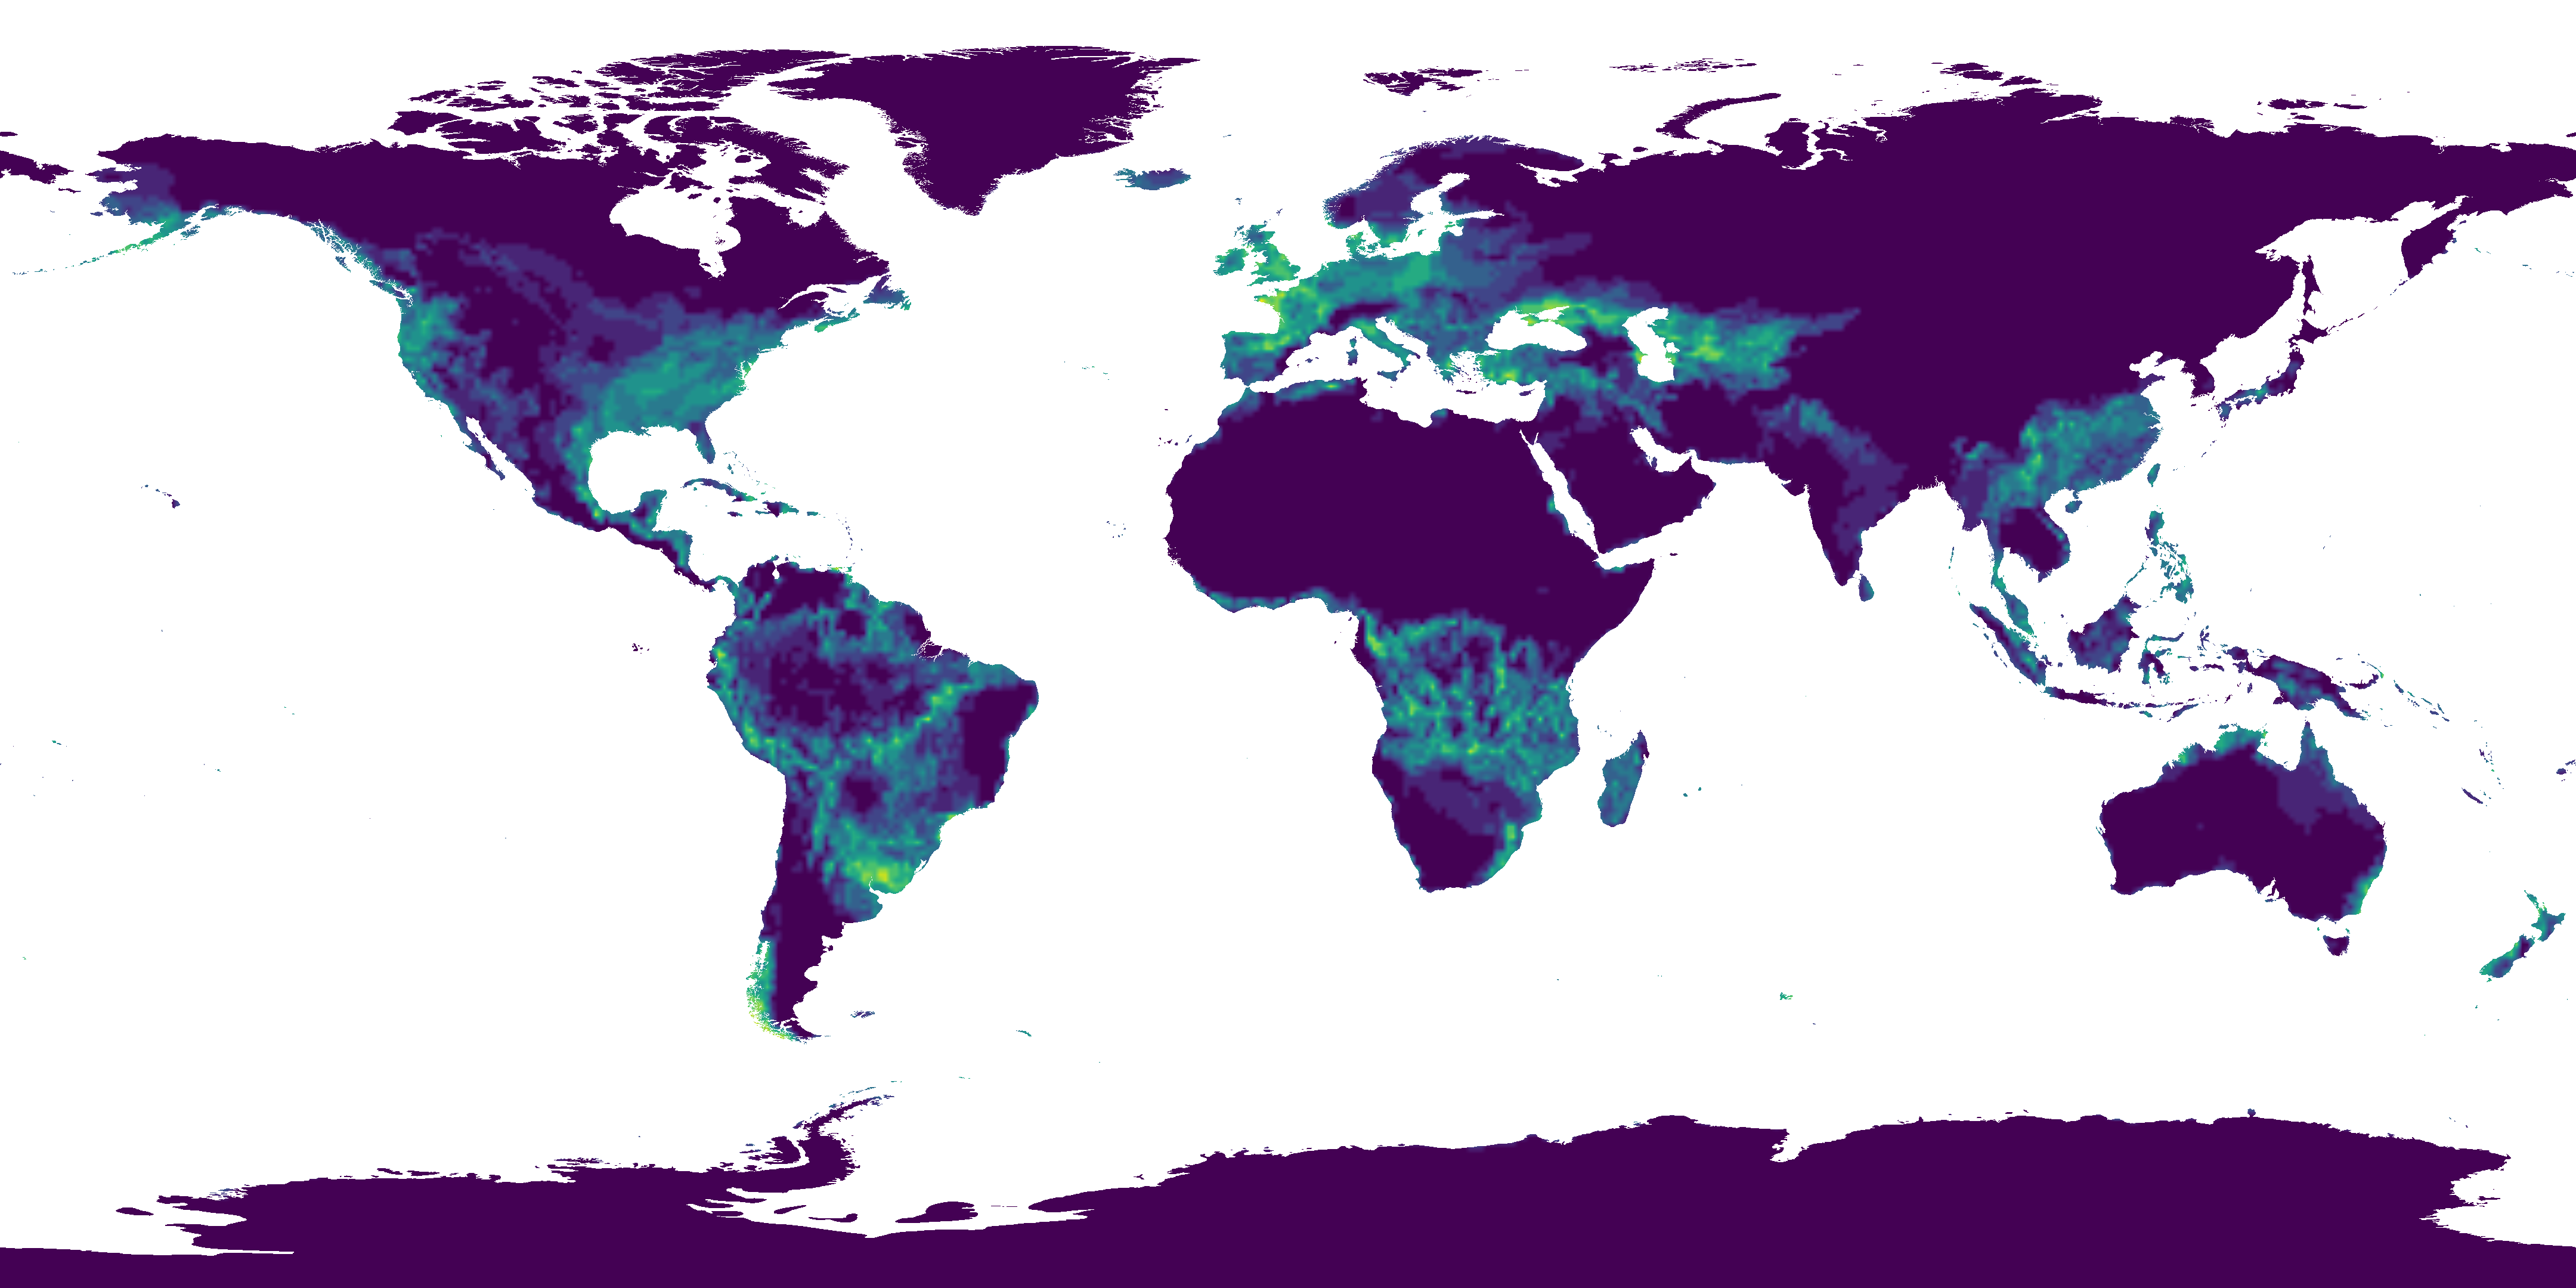
\includegraphics[width=.28\textwidth,height=2cm]{TOW_frequency_2019_01_cropped_rescaled_773f5b95_6131_4c82_814a_3675e7448be8.png}}\hfill
\subfloat[TOW February]{\label{sfig:b}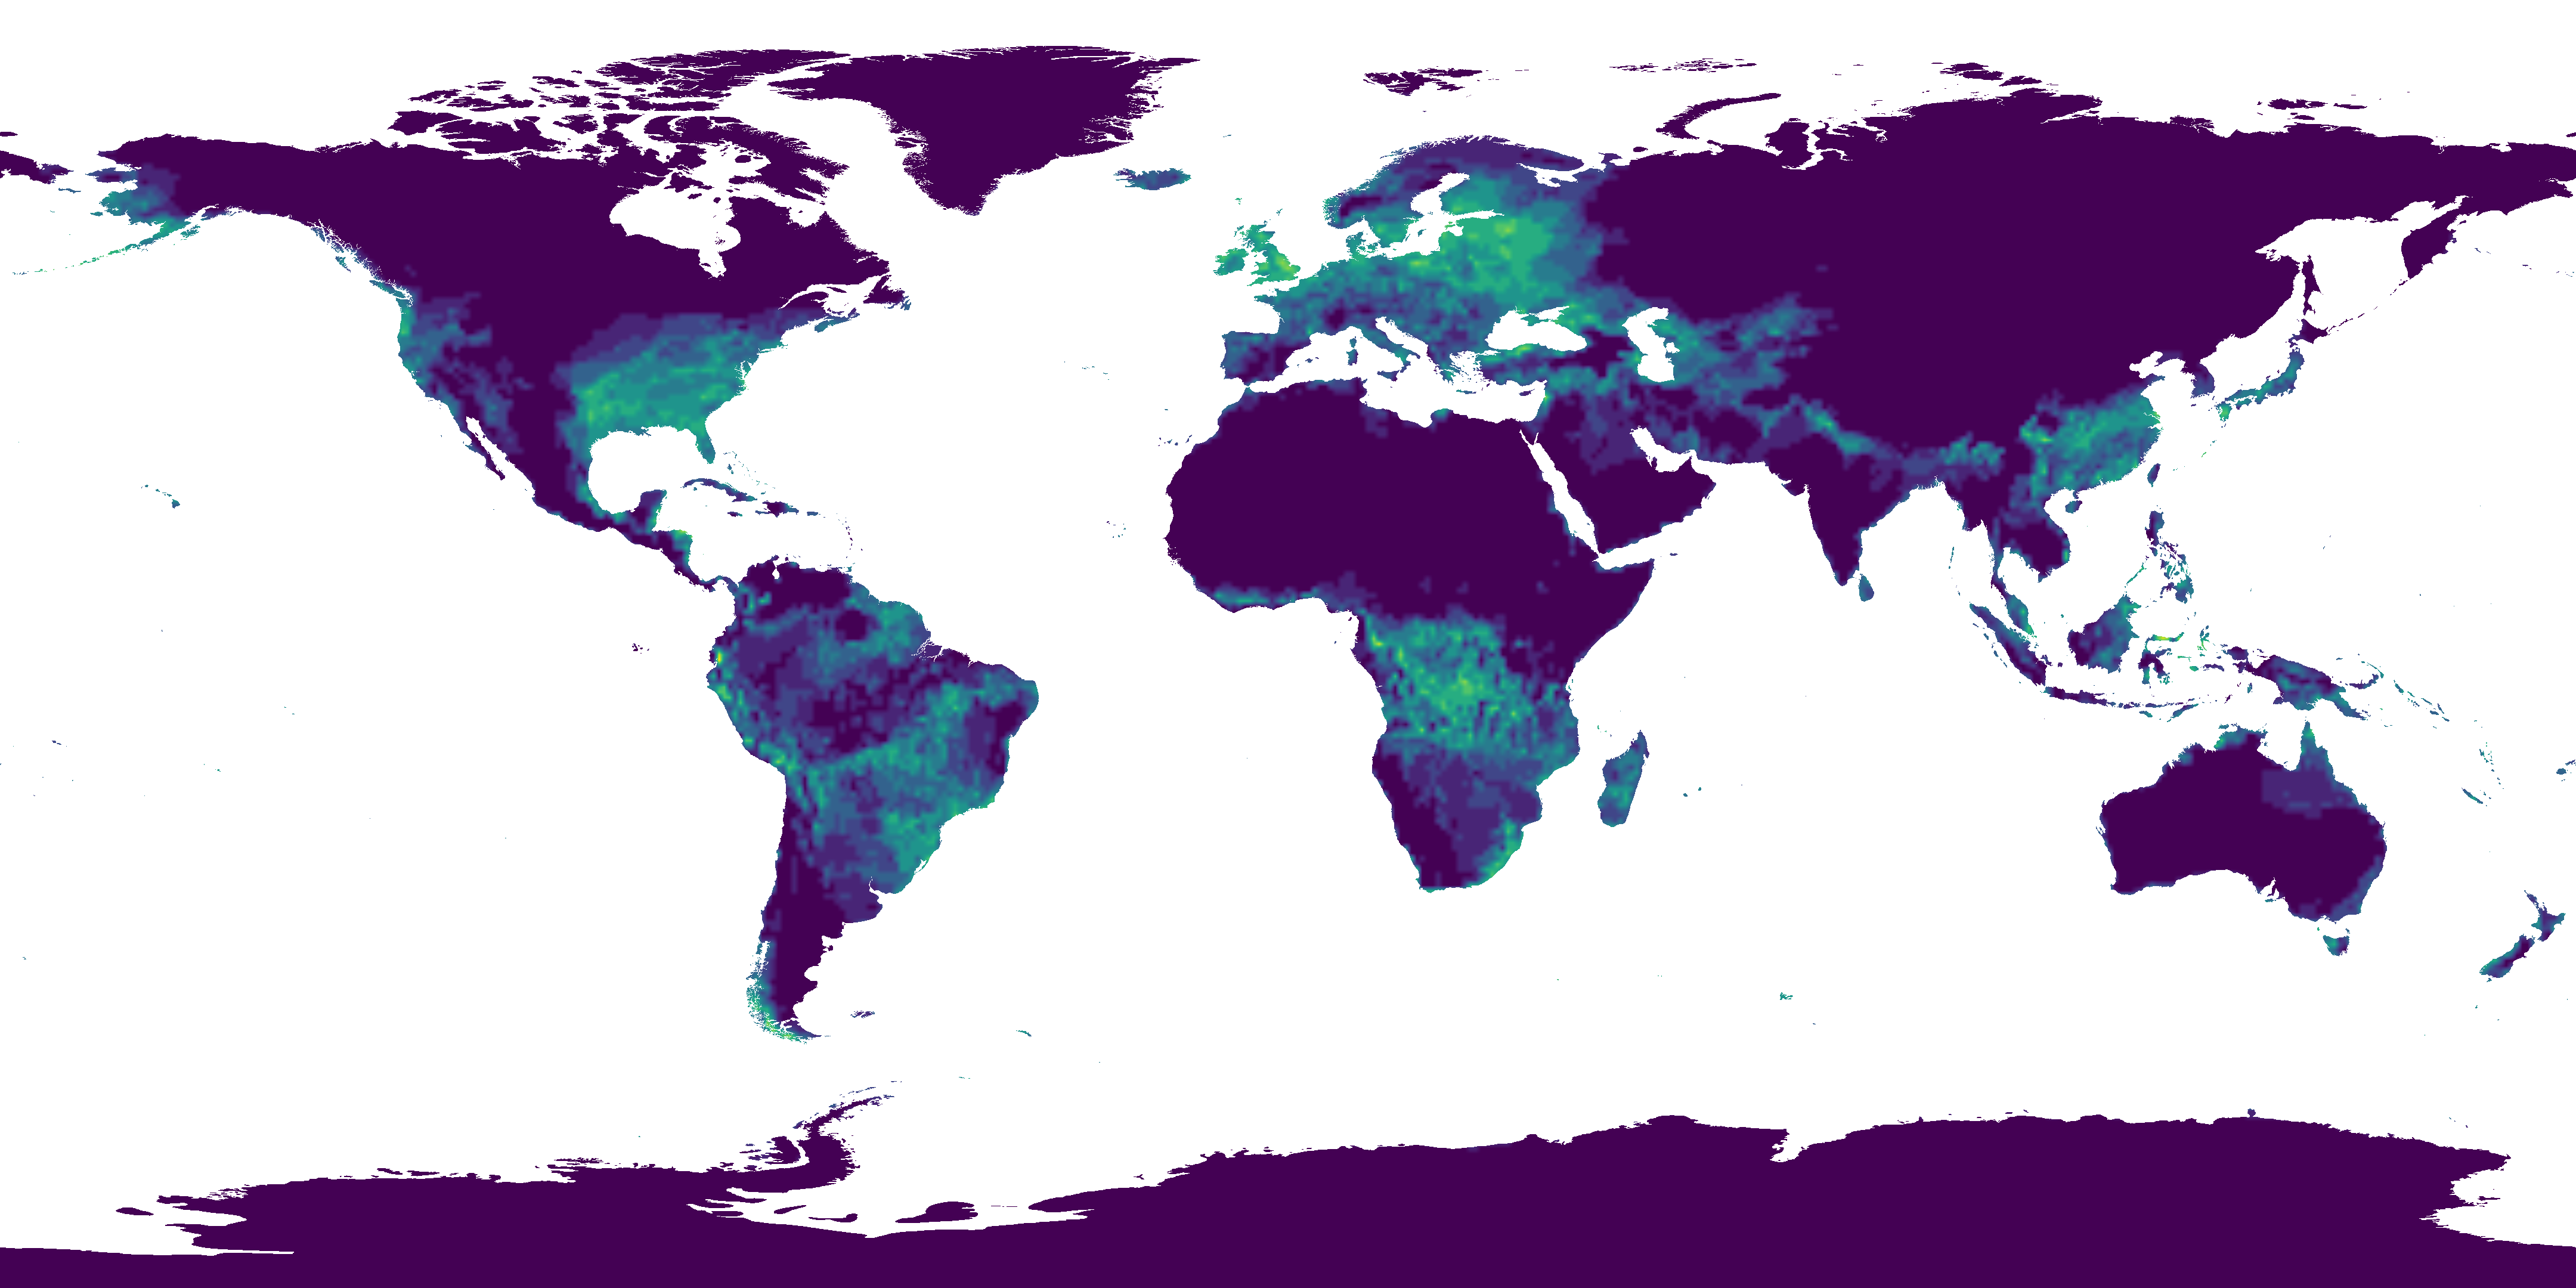
\includegraphics[width=.28\textwidth,height=2cm]{TOW_frequency_2019_02_cropped_rescaled_4bfa966a_bc33_45f1_8460_d550e5730f09.png}}\hfill
\subfloat[TOW March]{\label{sfig:c}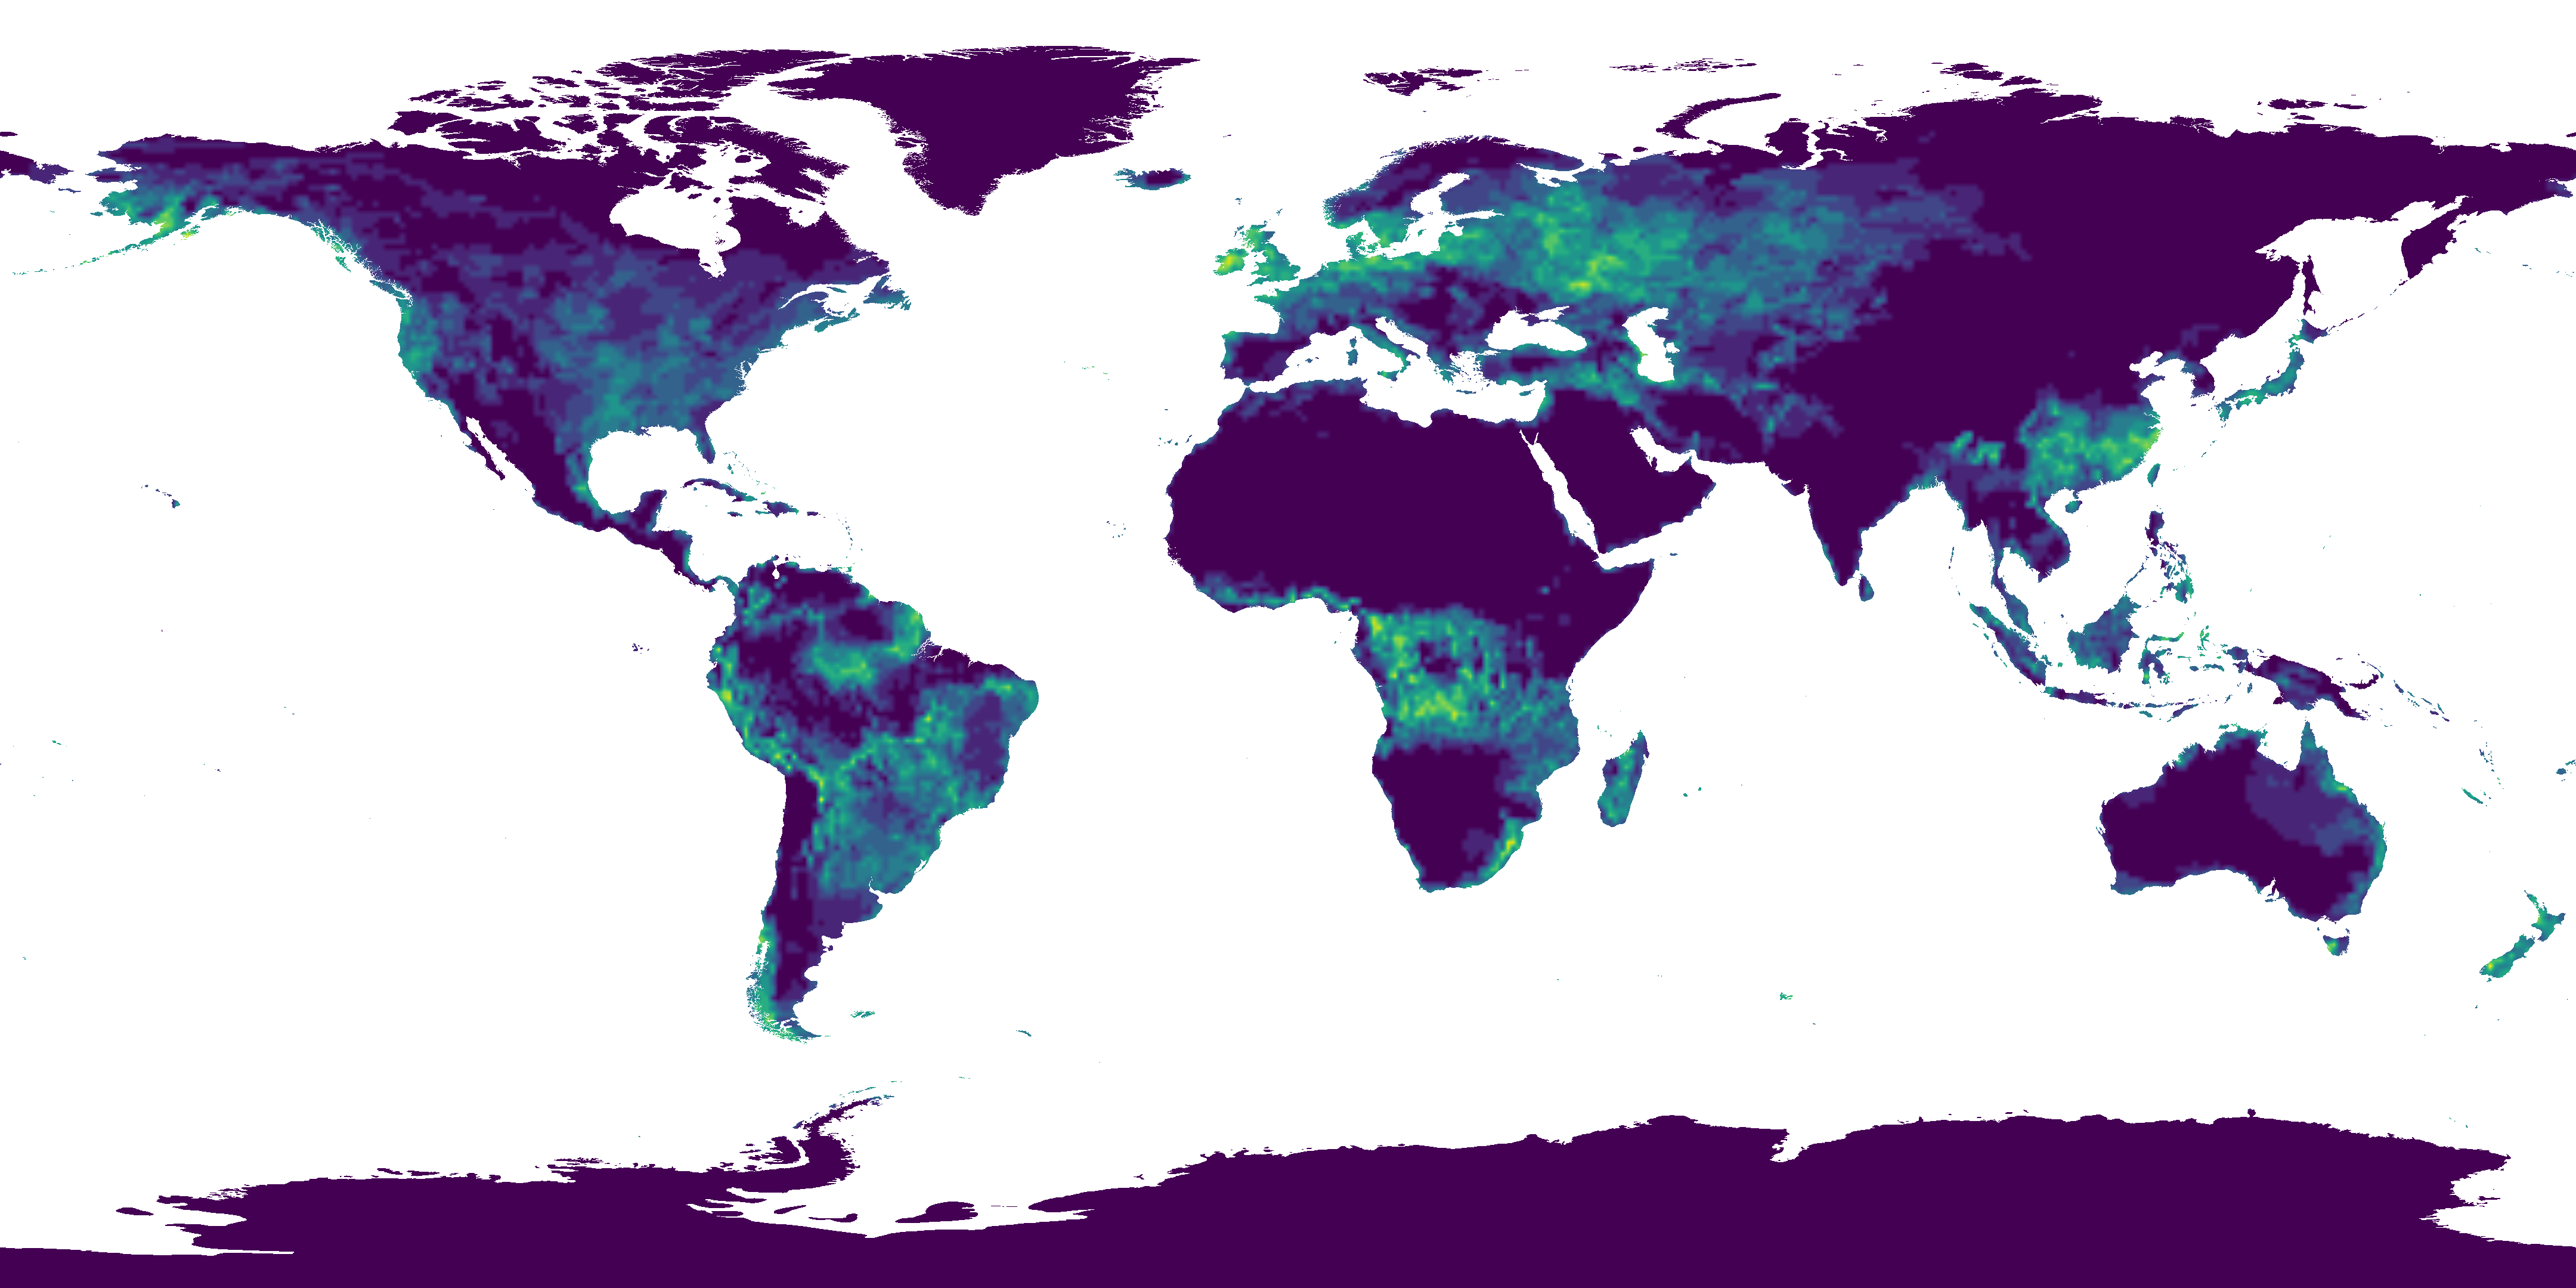
\includegraphics[width=.28\textwidth,height=2cm]{TOW_frequency_2019_03_cropped_rescaled_6455a31b_f777_4acf_9a64_70a50613a3c6.png}}\\
\subfloat[TOW April]{\label{sfig:d}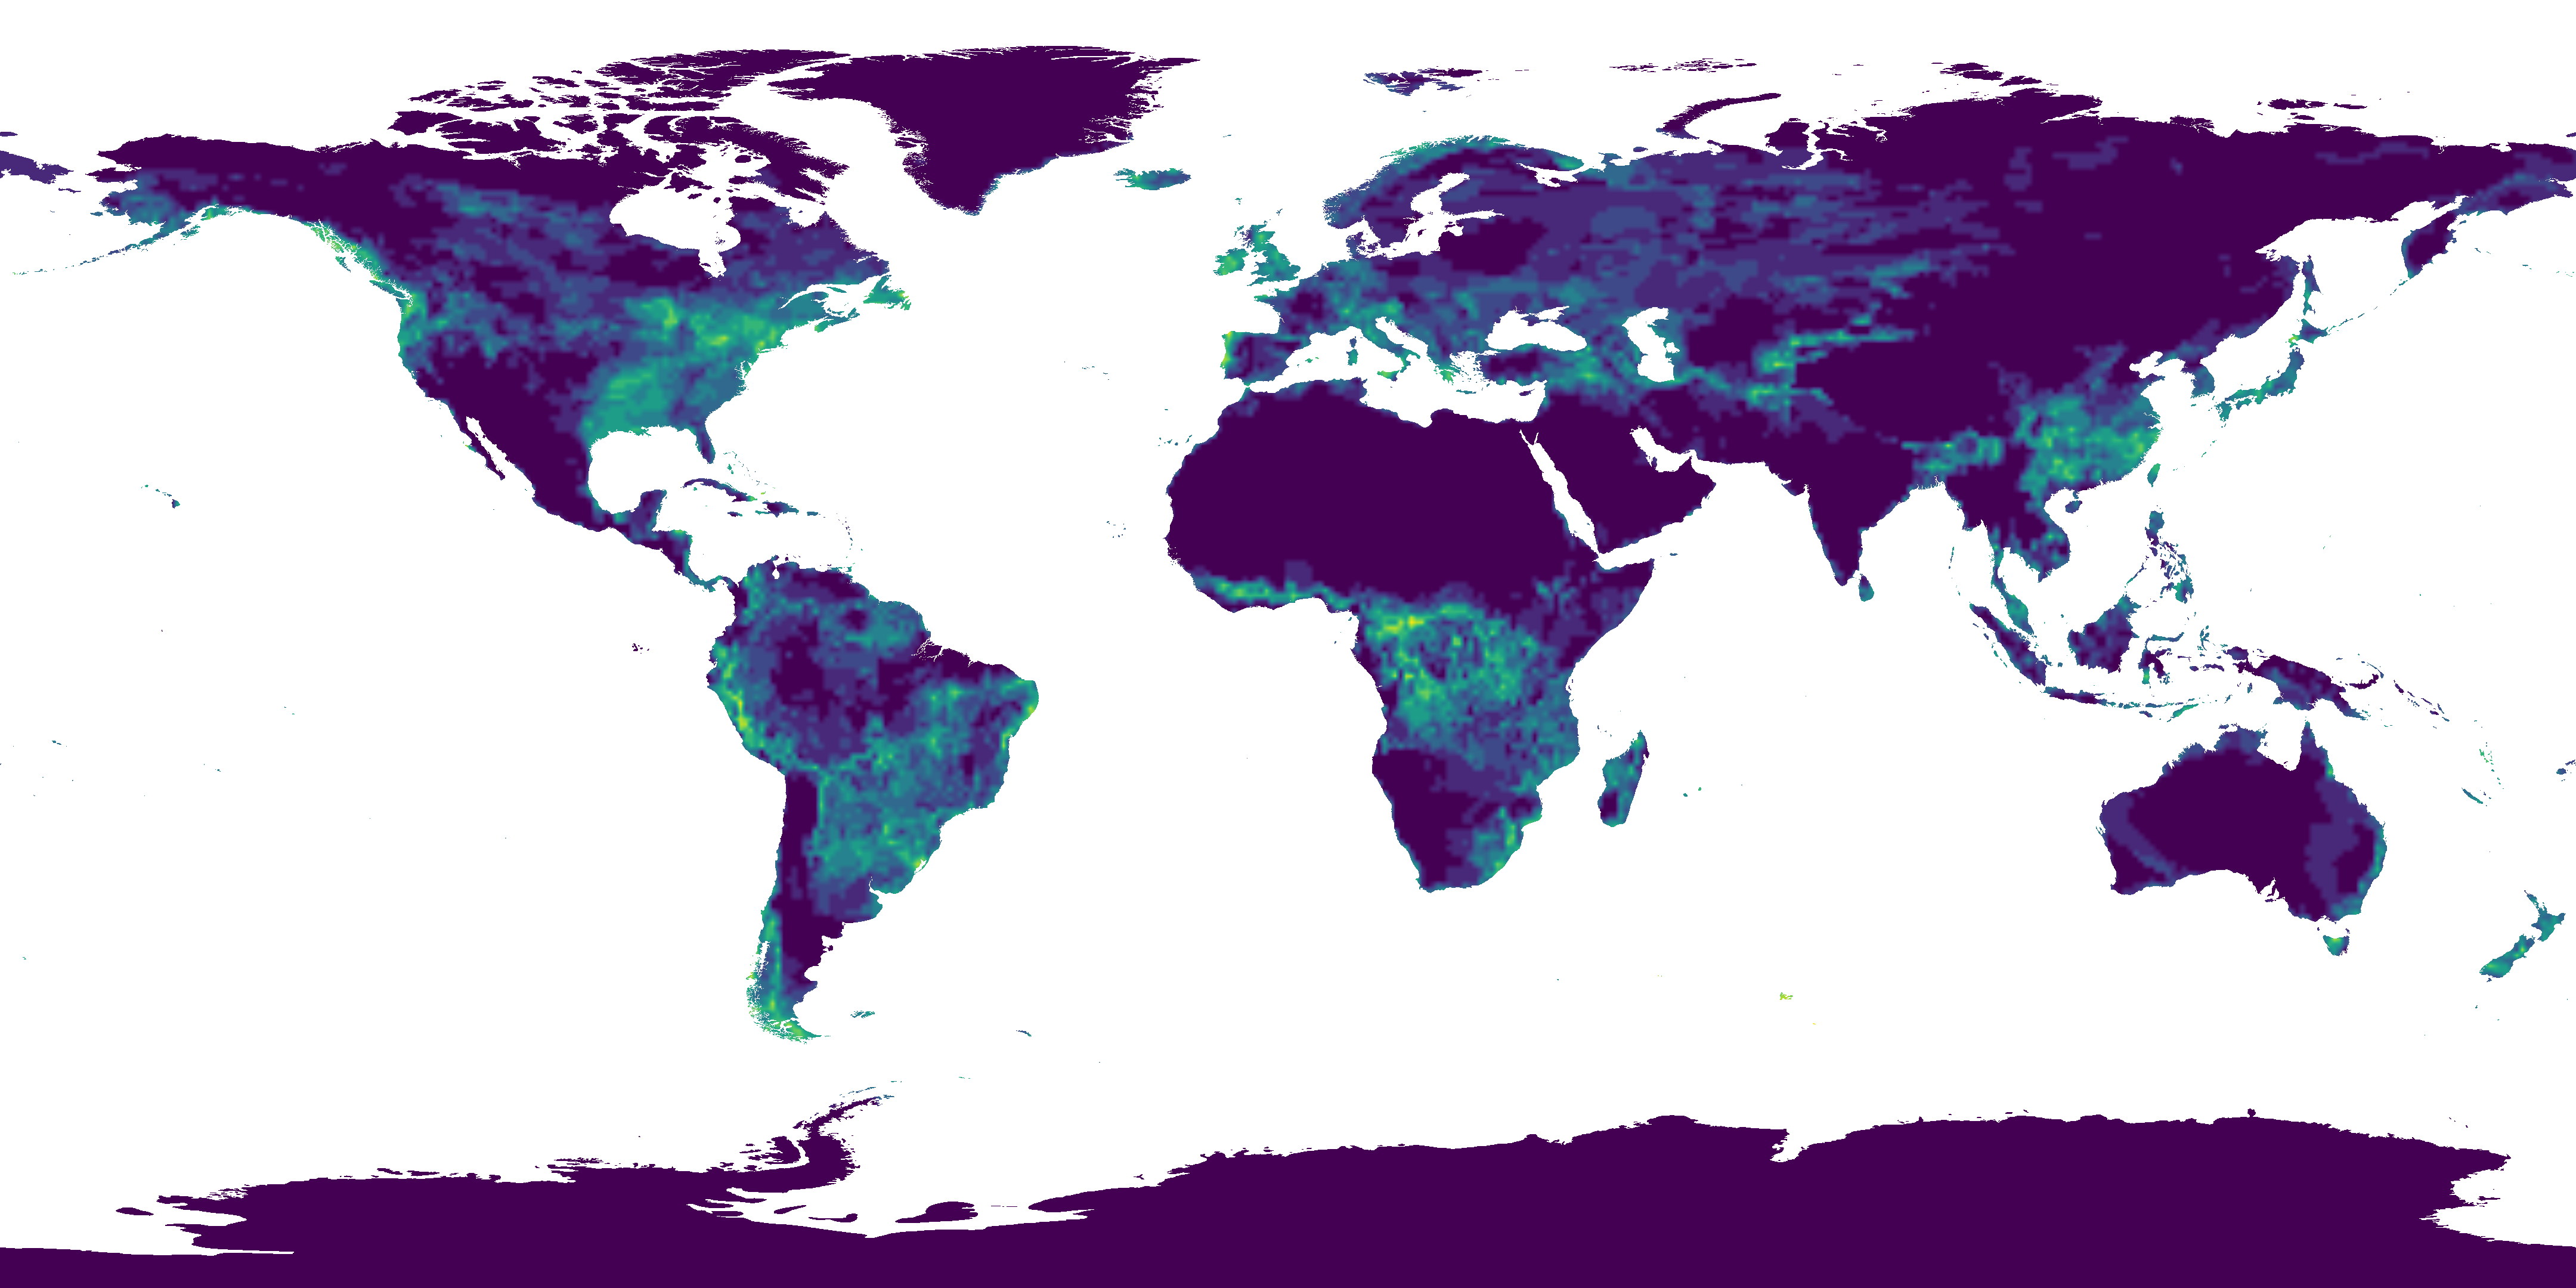
\includegraphics[width=.28\textwidth,height=2cm]{TOW_frequency_2019_04_cropped_rescaled_e4e0d24f_1dd2_4eca_9238_2e51a1a2eec8.png}}\hfill
\subfloat[TOW May]{\label{sfig:e}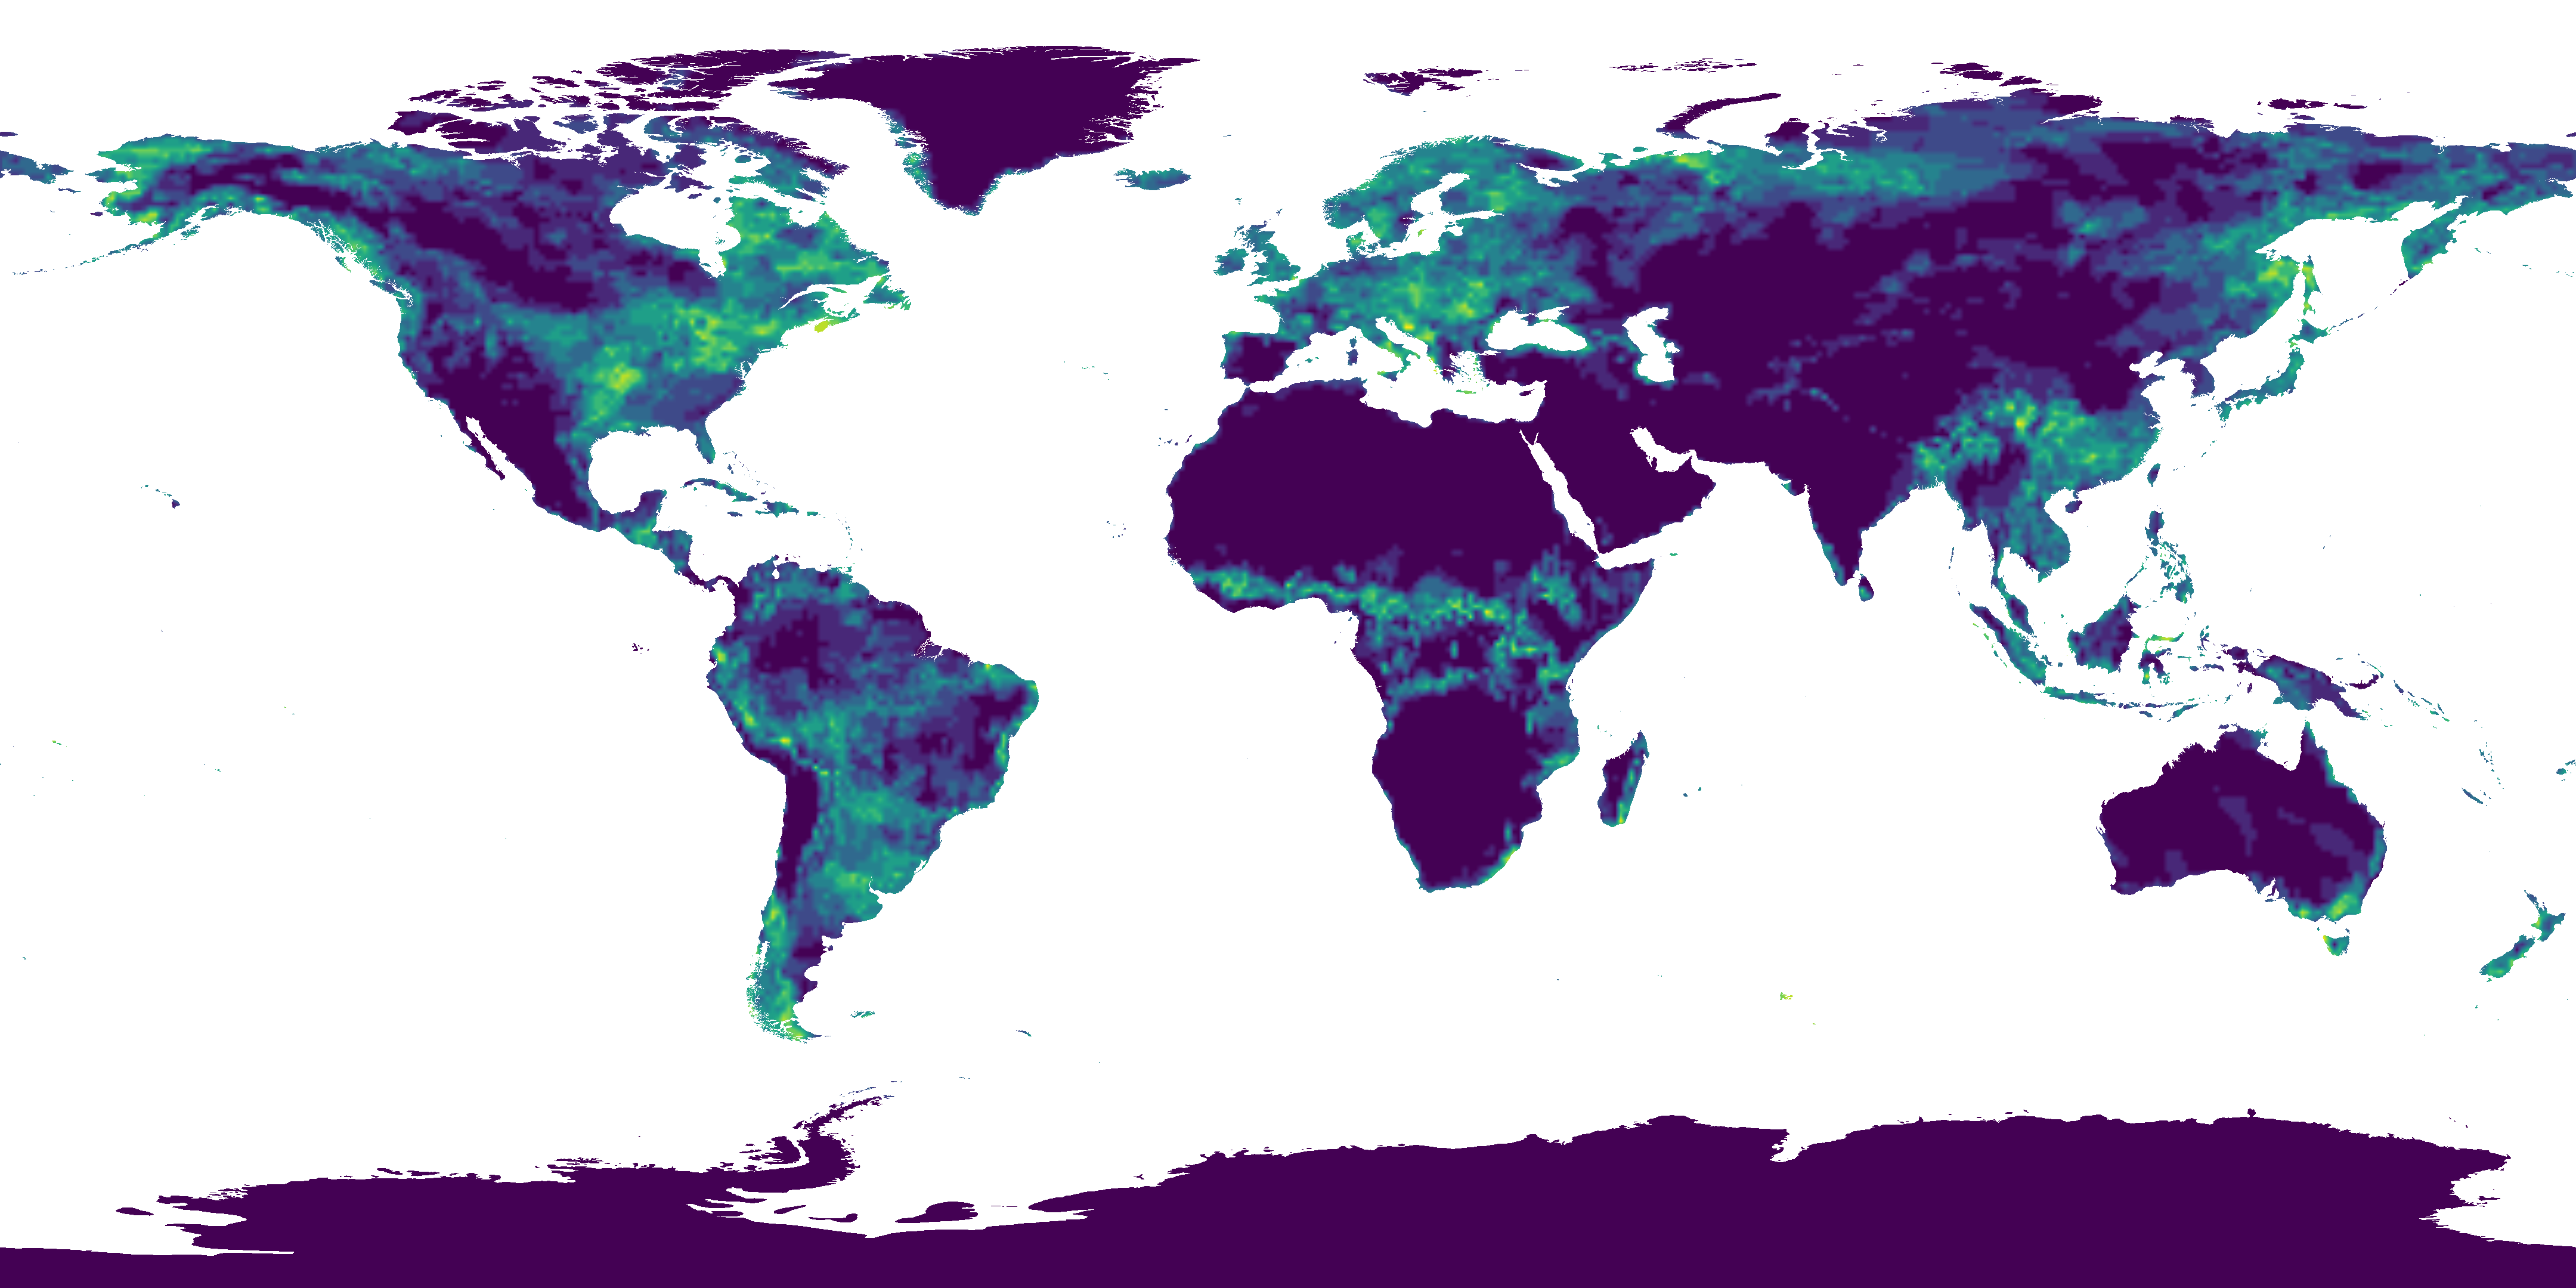
\includegraphics[width=.28\textwidth,height=2cm]{TOW_frequency_2019_05_cropped_rescaled_61bc7028_781f_4dfb_87eb_88a32efc9140.png}}\hfill
\subfloat[TOW June]{\label{sfig:f}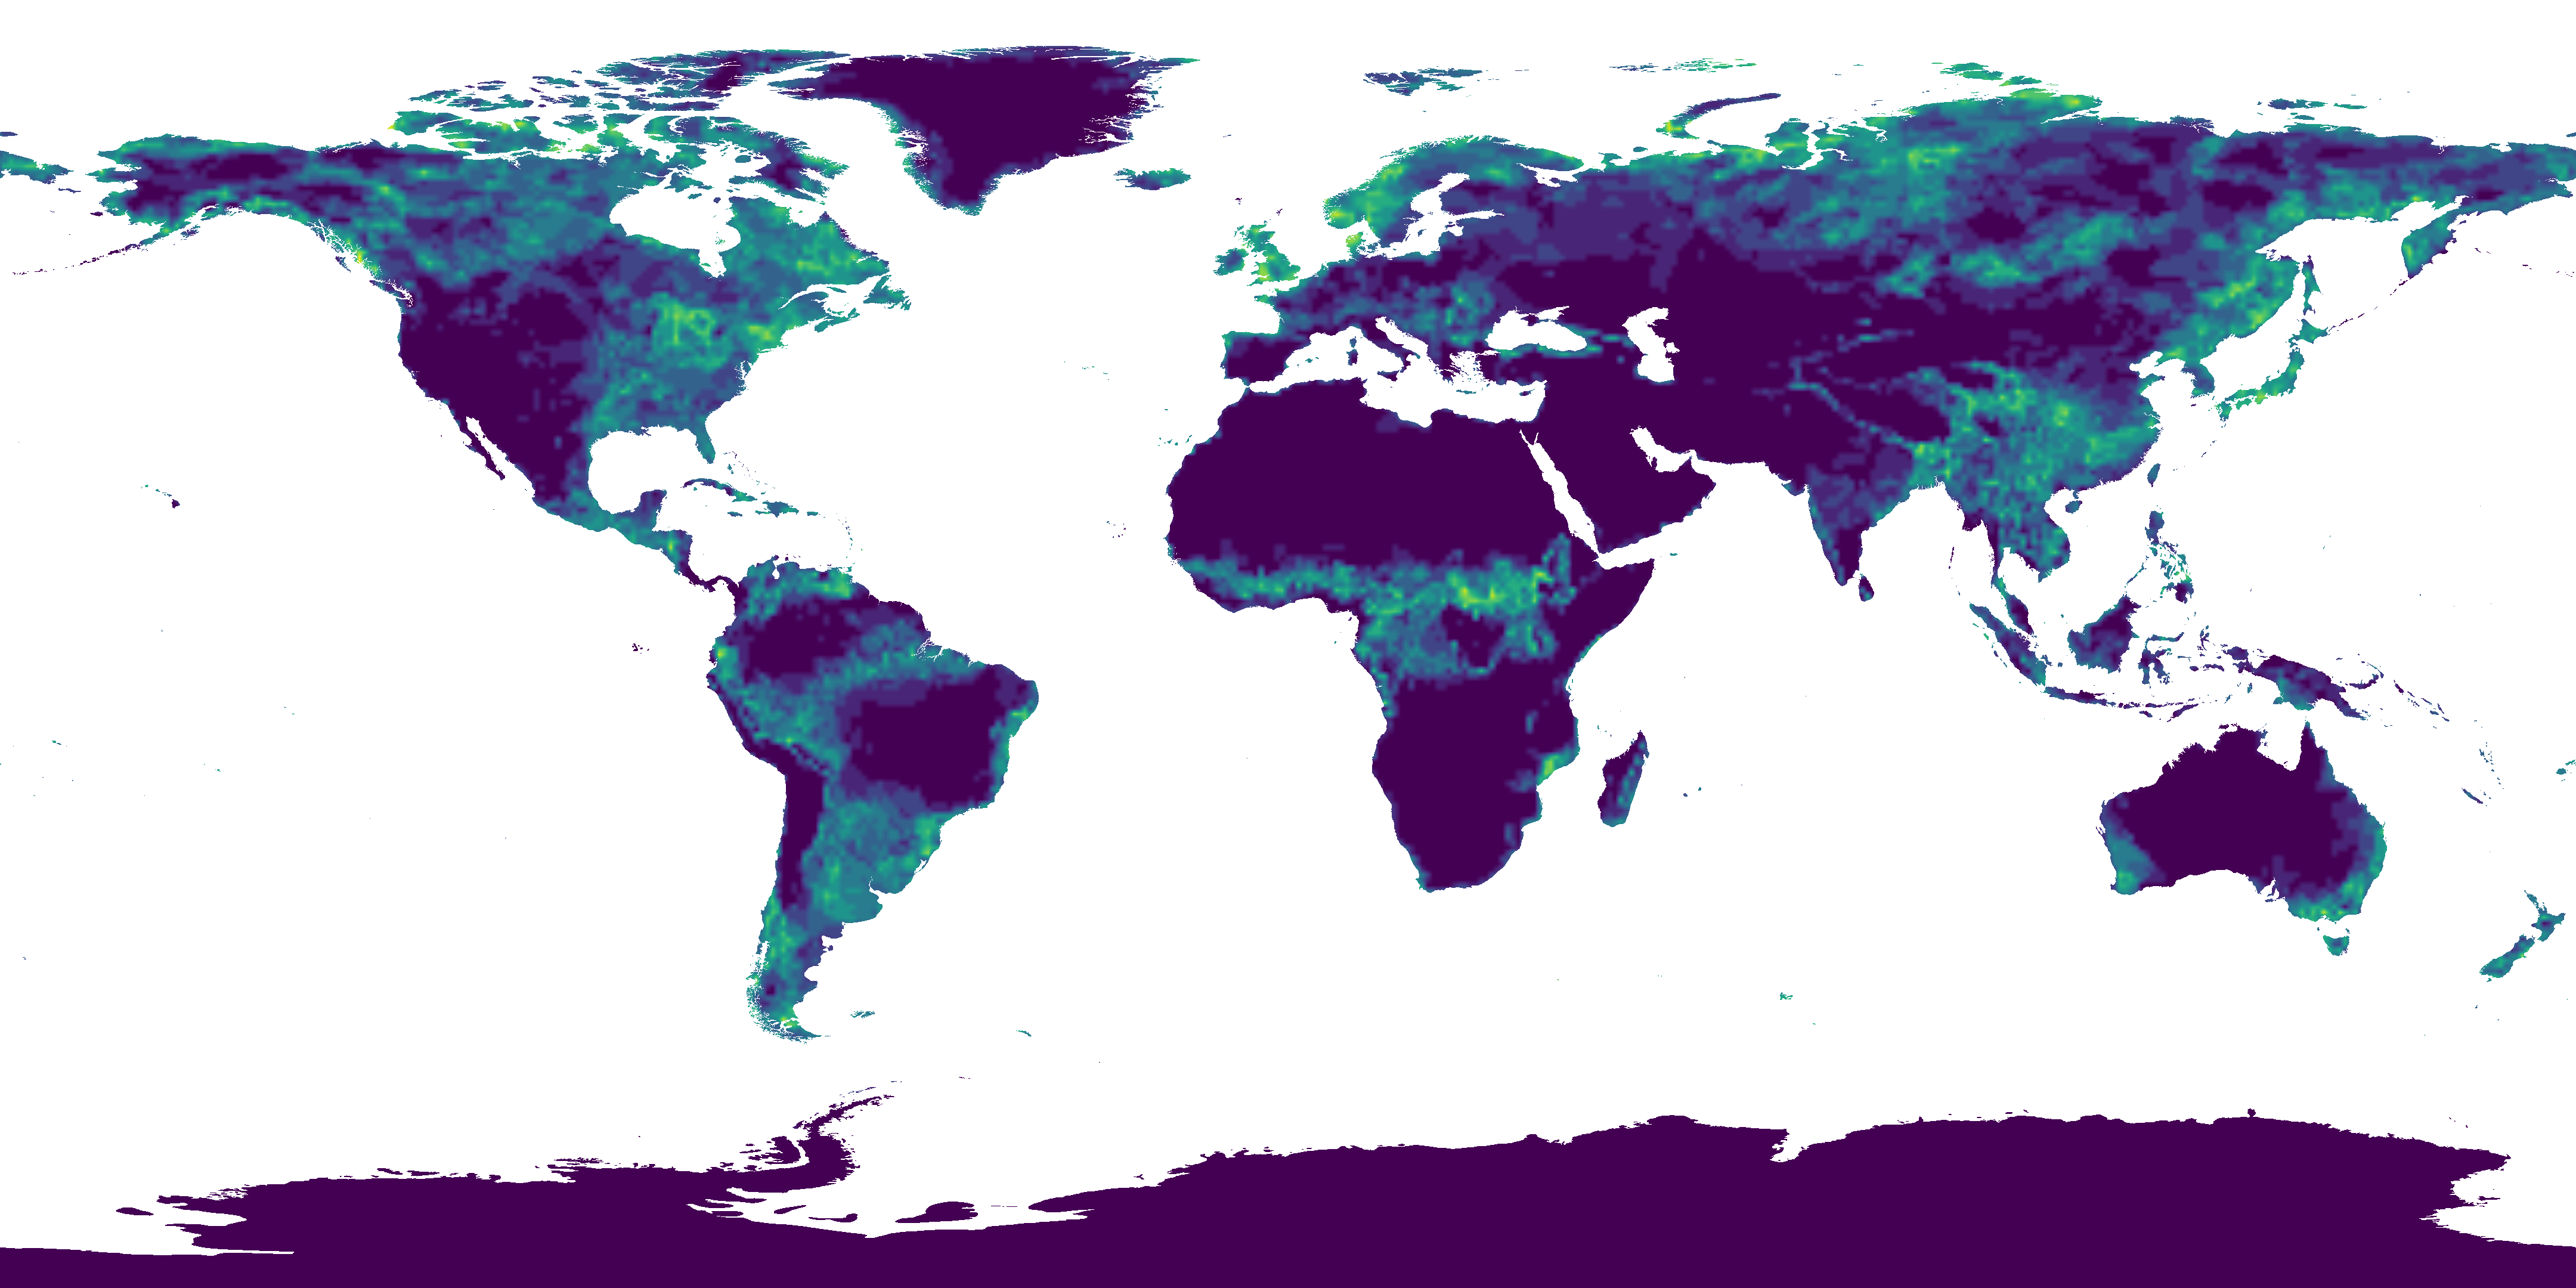
\includegraphics[width=.28\textwidth,height=2cm]{TOW_frequency_2019_06_cropped_rescaled_2967ac56_6f59_4516_bae1_422f6d97f12a.png}}\\
\subfloat[TOW July]{\label{sfig:a}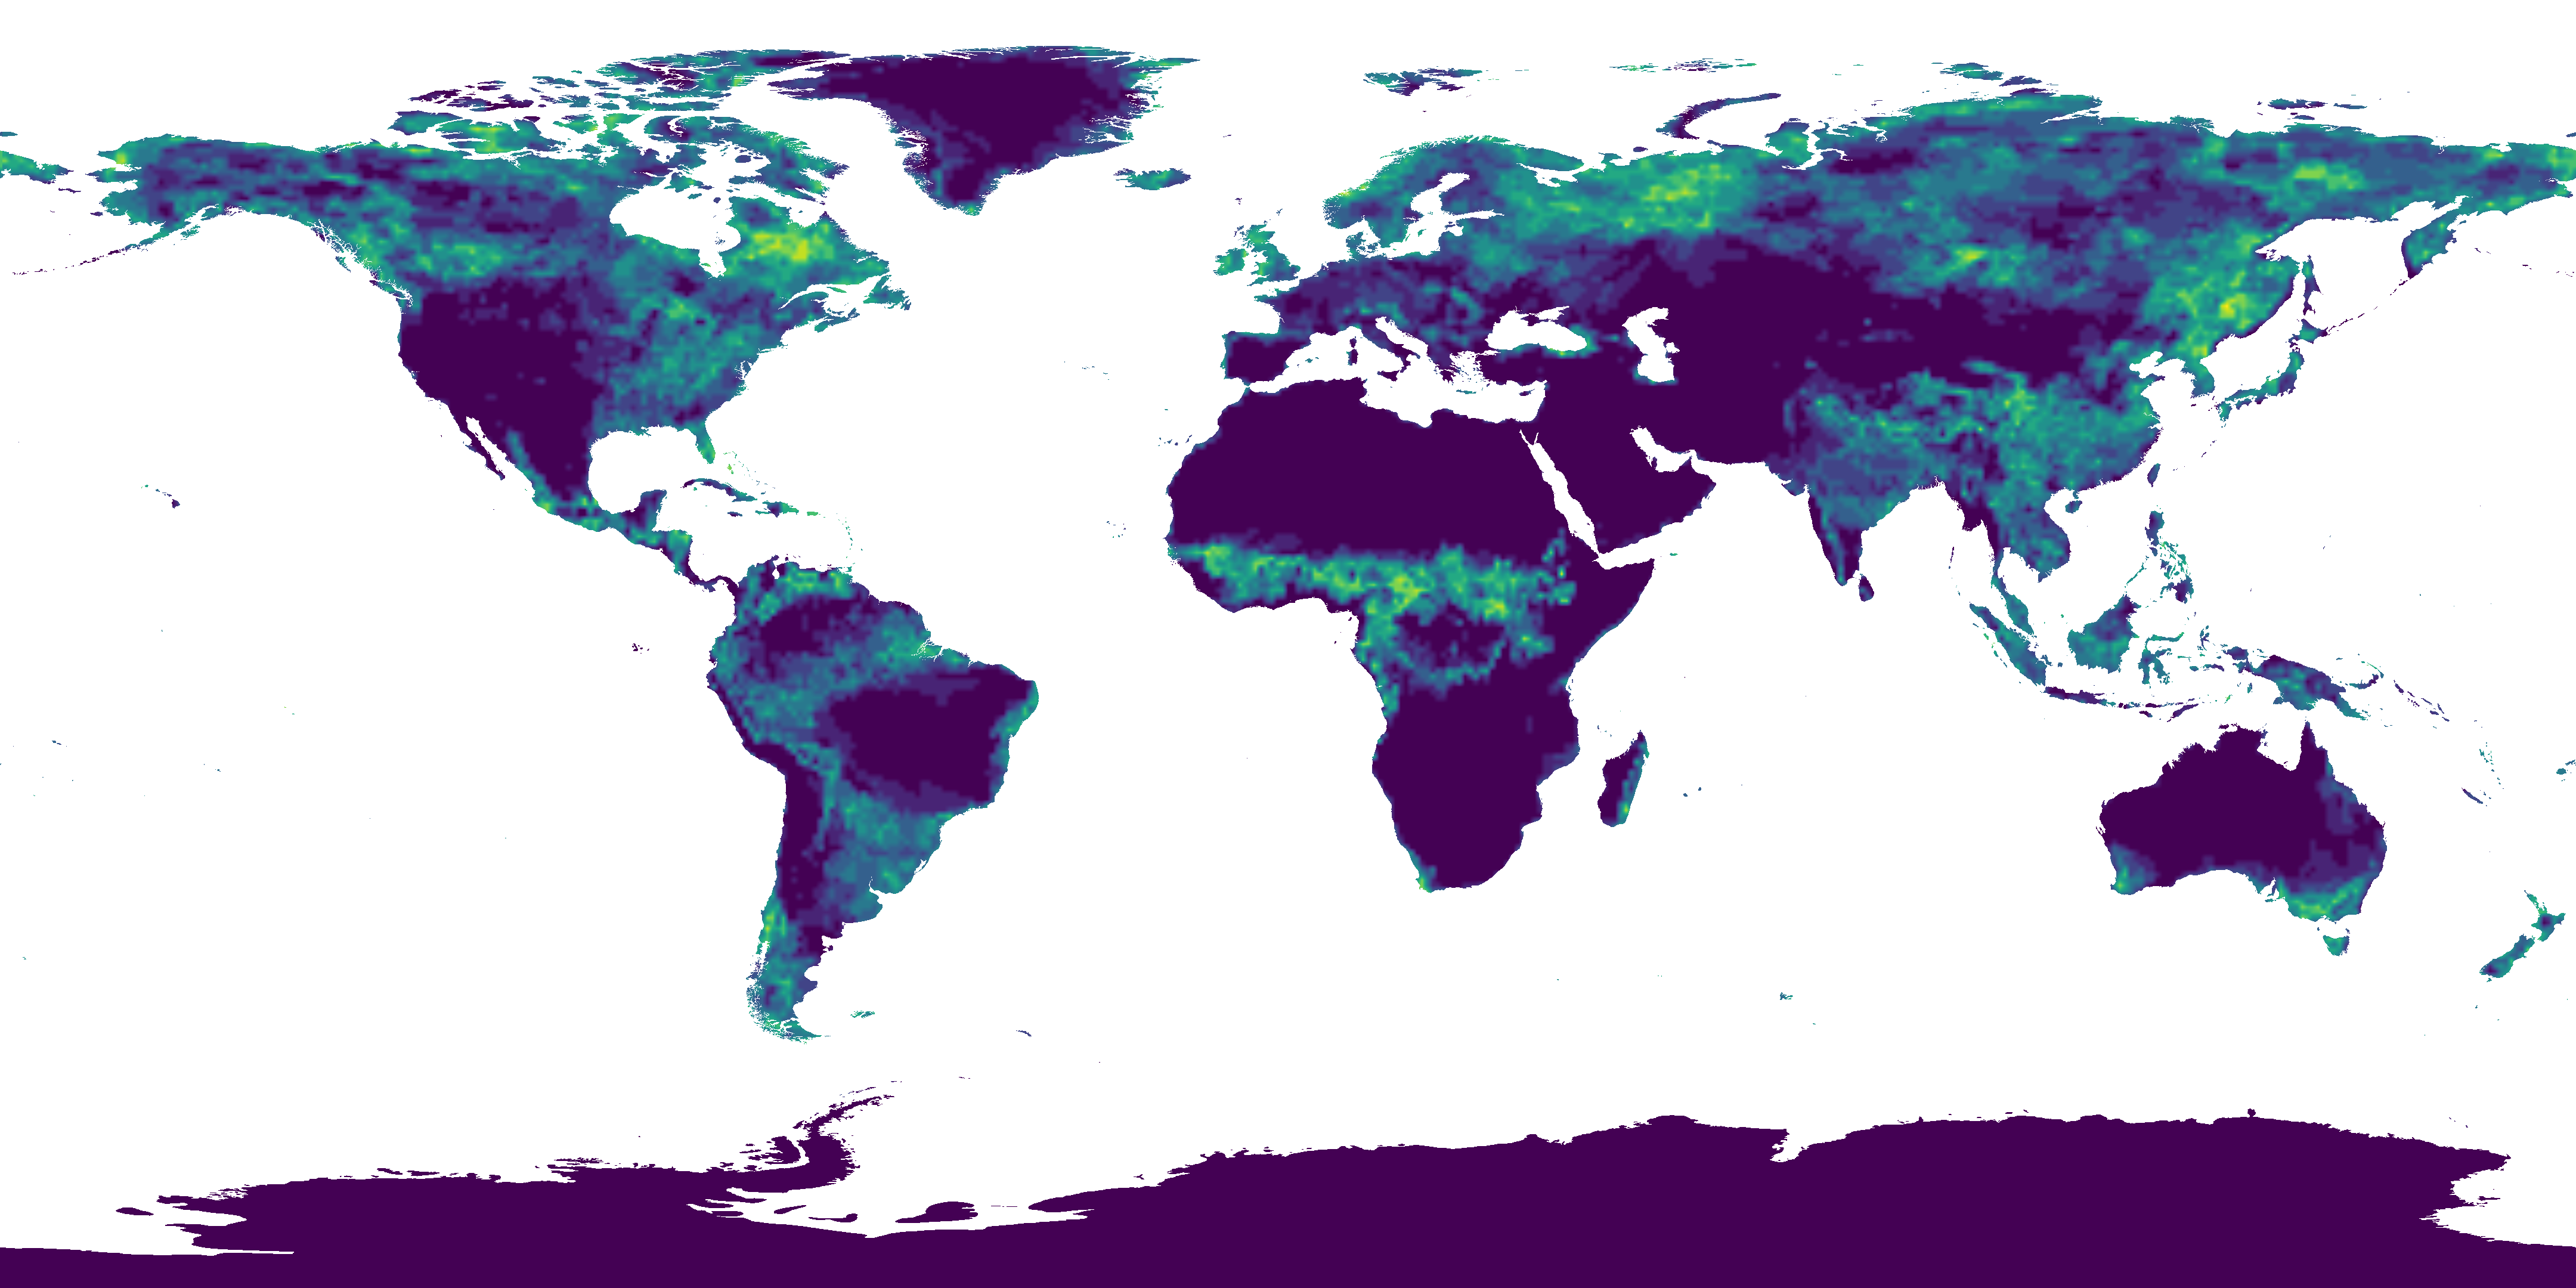
\includegraphics[width=.28\textwidth,height=2cm]{TOW_frequency_2019_07_cropped_rescaled_0a63ecd9_e7e7_4487_97c3_d185f6dff13b.png}}\hfill
\subfloat[TOW August]{\label{sfig:b}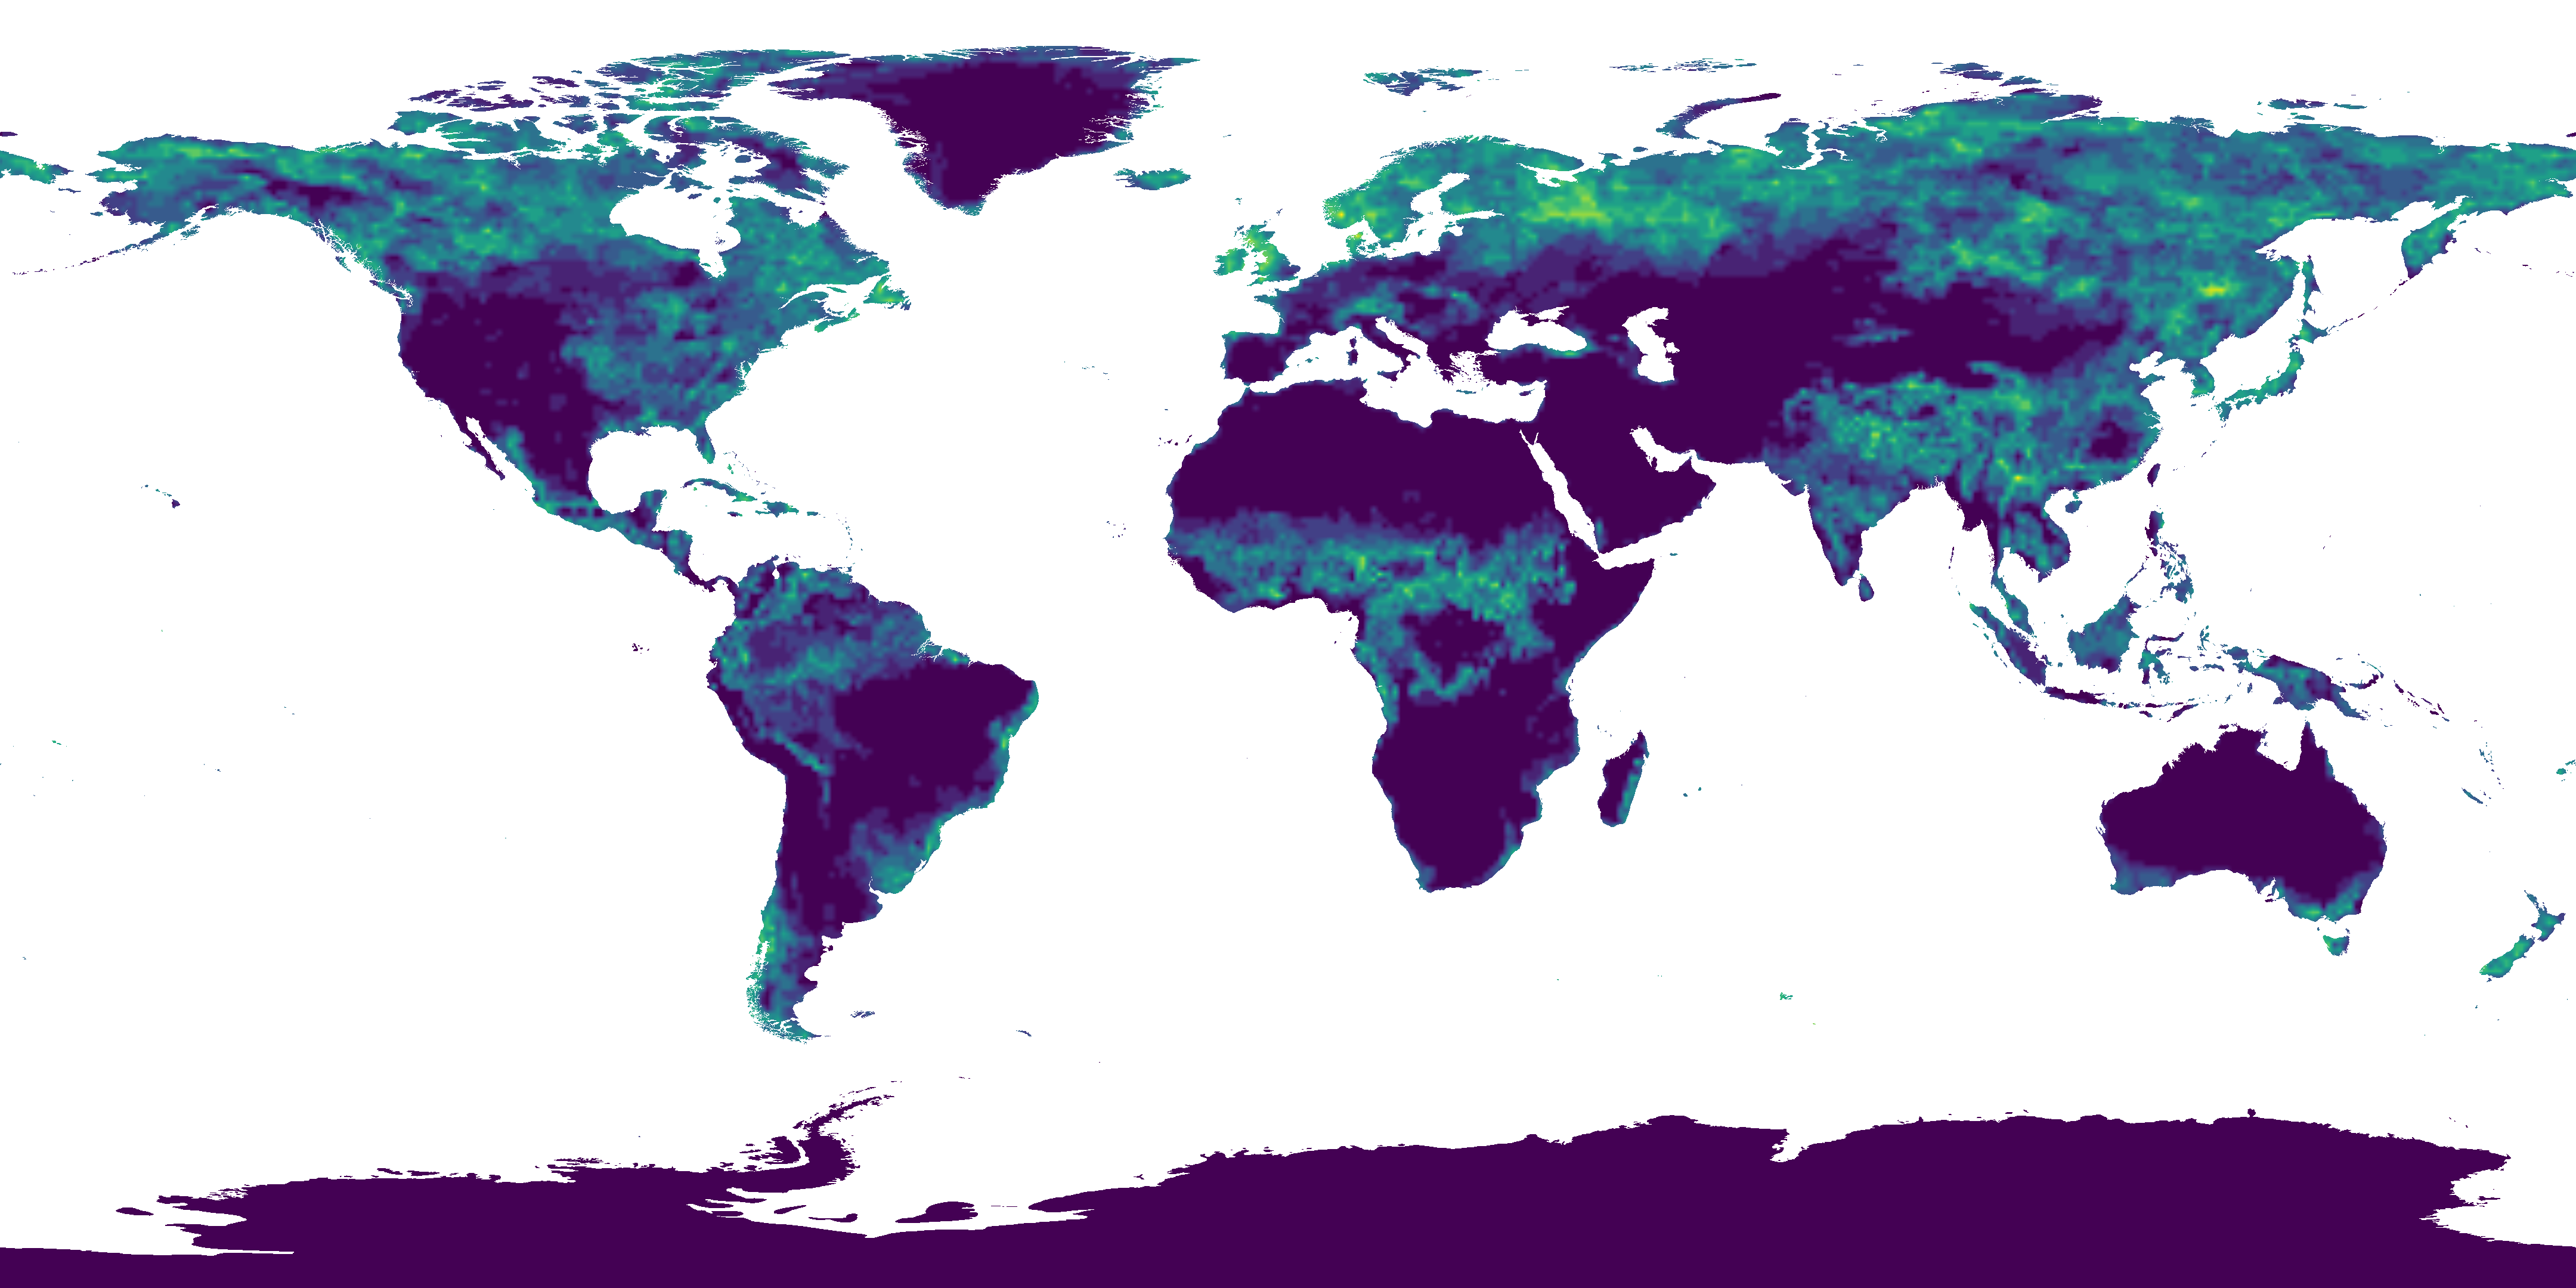
\includegraphics[width=.28\textwidth,height=2cm]{TOW_frequency_2019_08_cropped_rescaled_76f4fd09_21a7_485b_9f00_29d382569b8c.png}}\hfill
\subfloat[TOW September]{\label{sfig:c}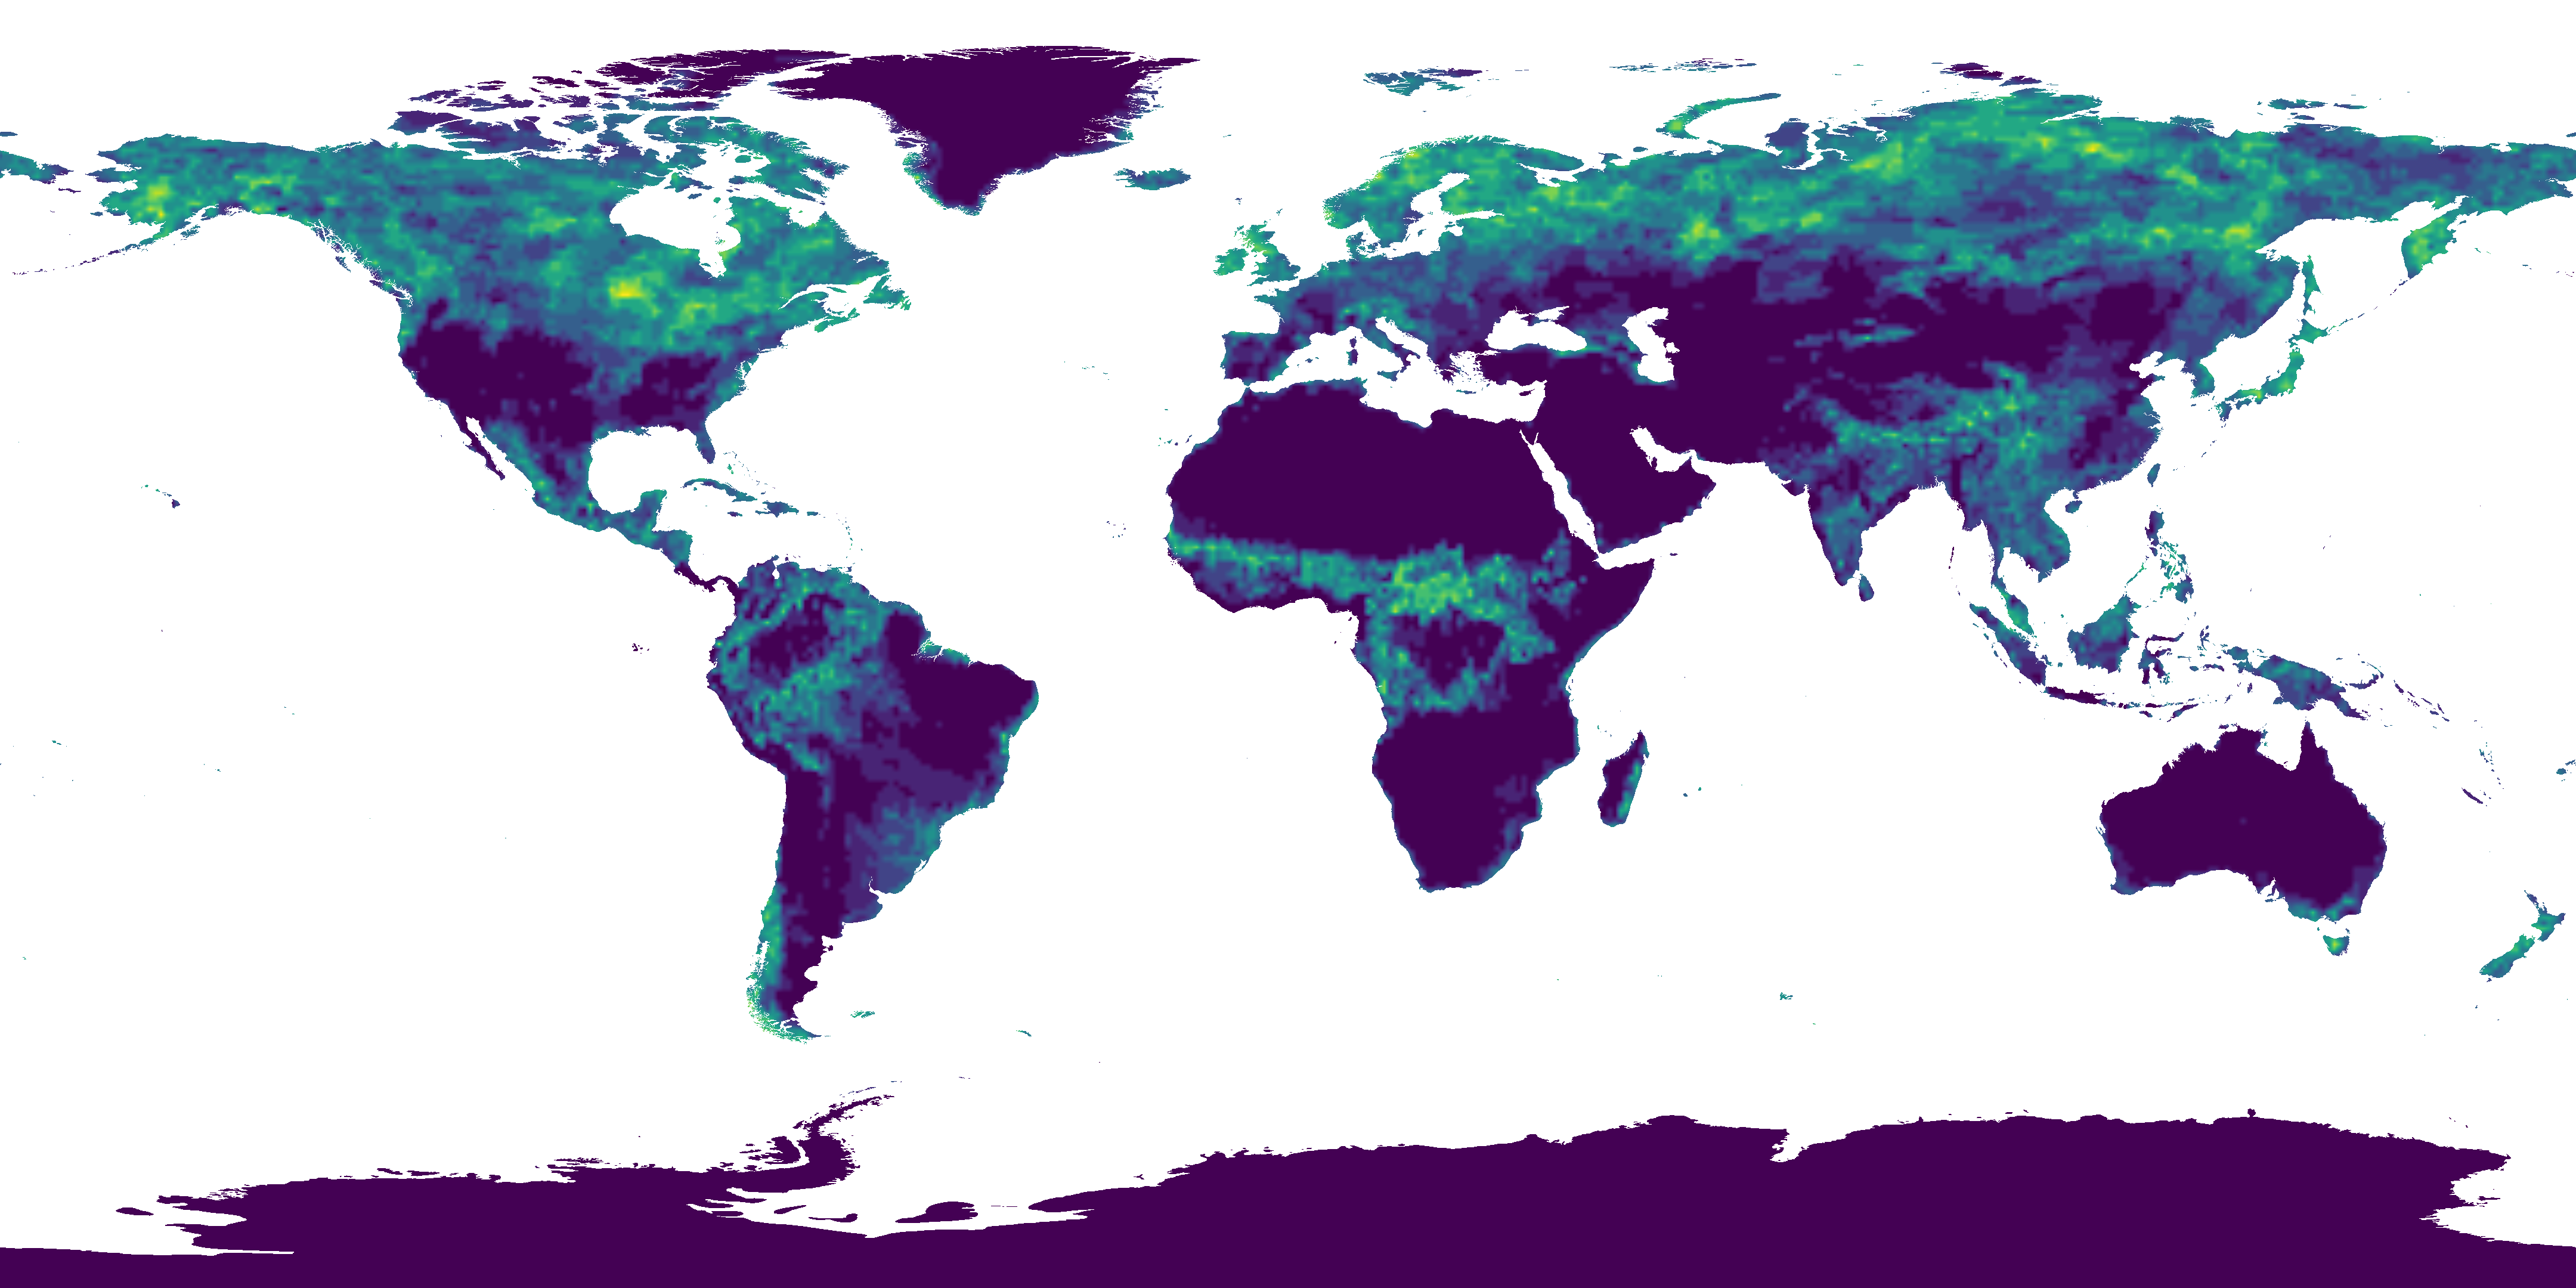
\includegraphics[width=.28\textwidth,height=2cm]{TOW_frequency_2019_09_cropped_rescaled_dce2a392_797f_4b10_b4ad_70f95bc2e39e.png}}\\
\subfloat[TOW October]{\label{sfig:d}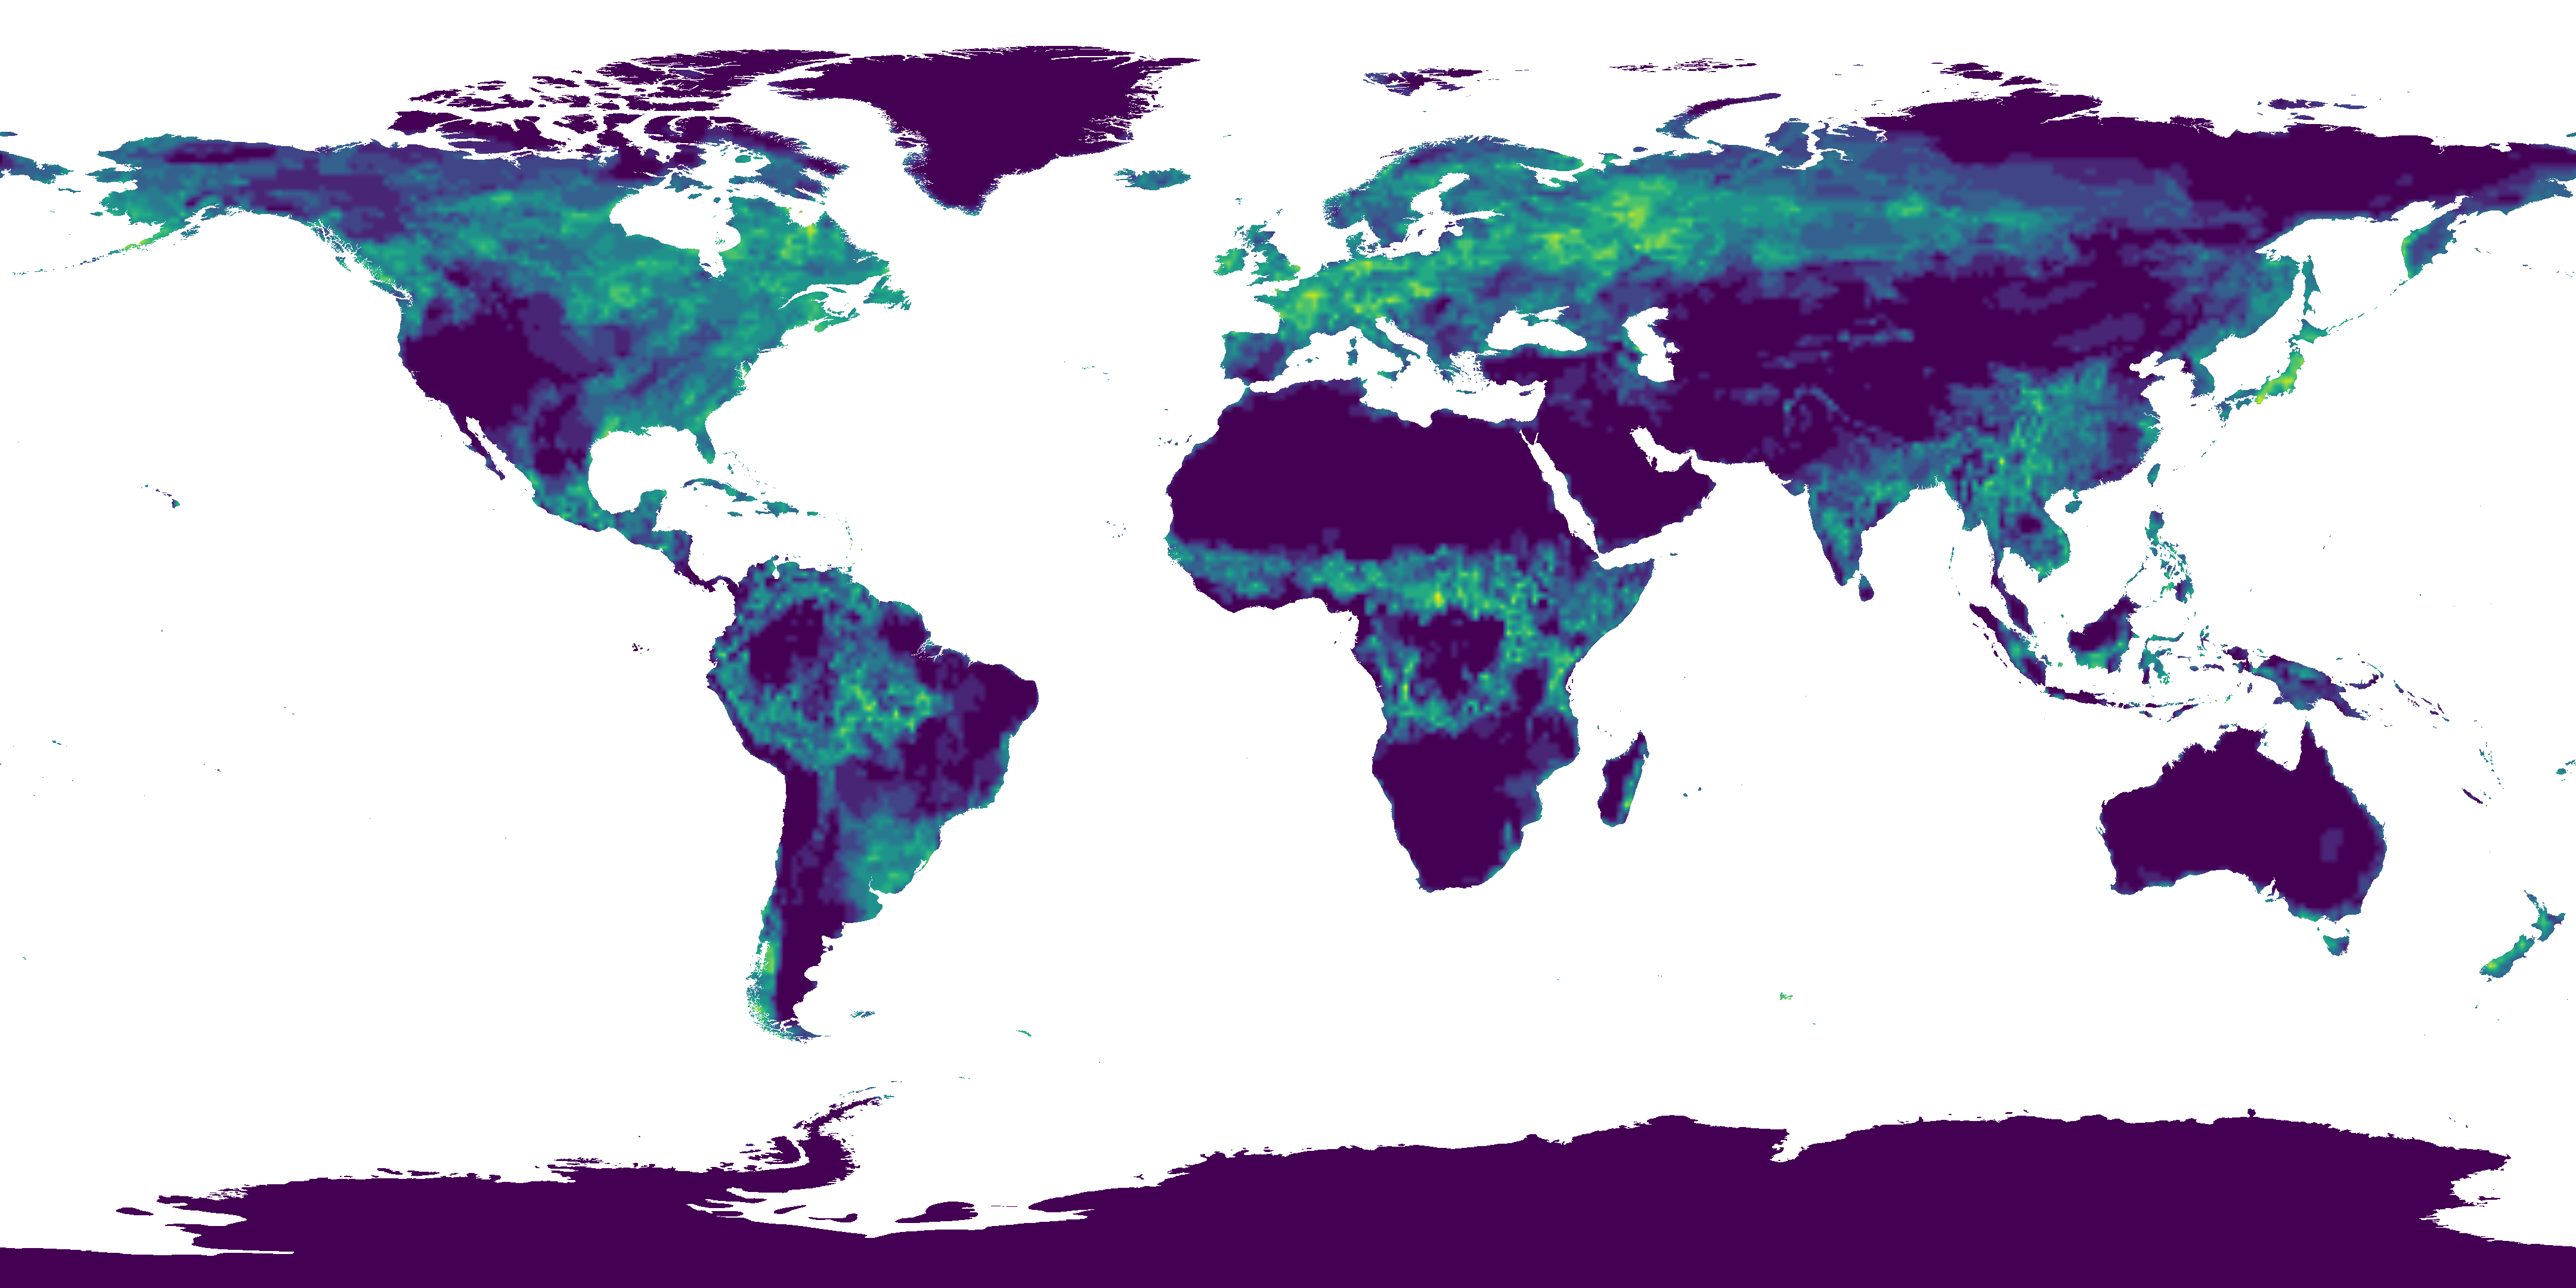
\includegraphics[width=.28\textwidth,height=2cm]{TOW_frequency_2019_10_cropped_rescaled_8ec534df_23dc_4735_a08f_d928db86a5b3.png}}\hfill
\subfloat[TOW November]{\label{sfig:e}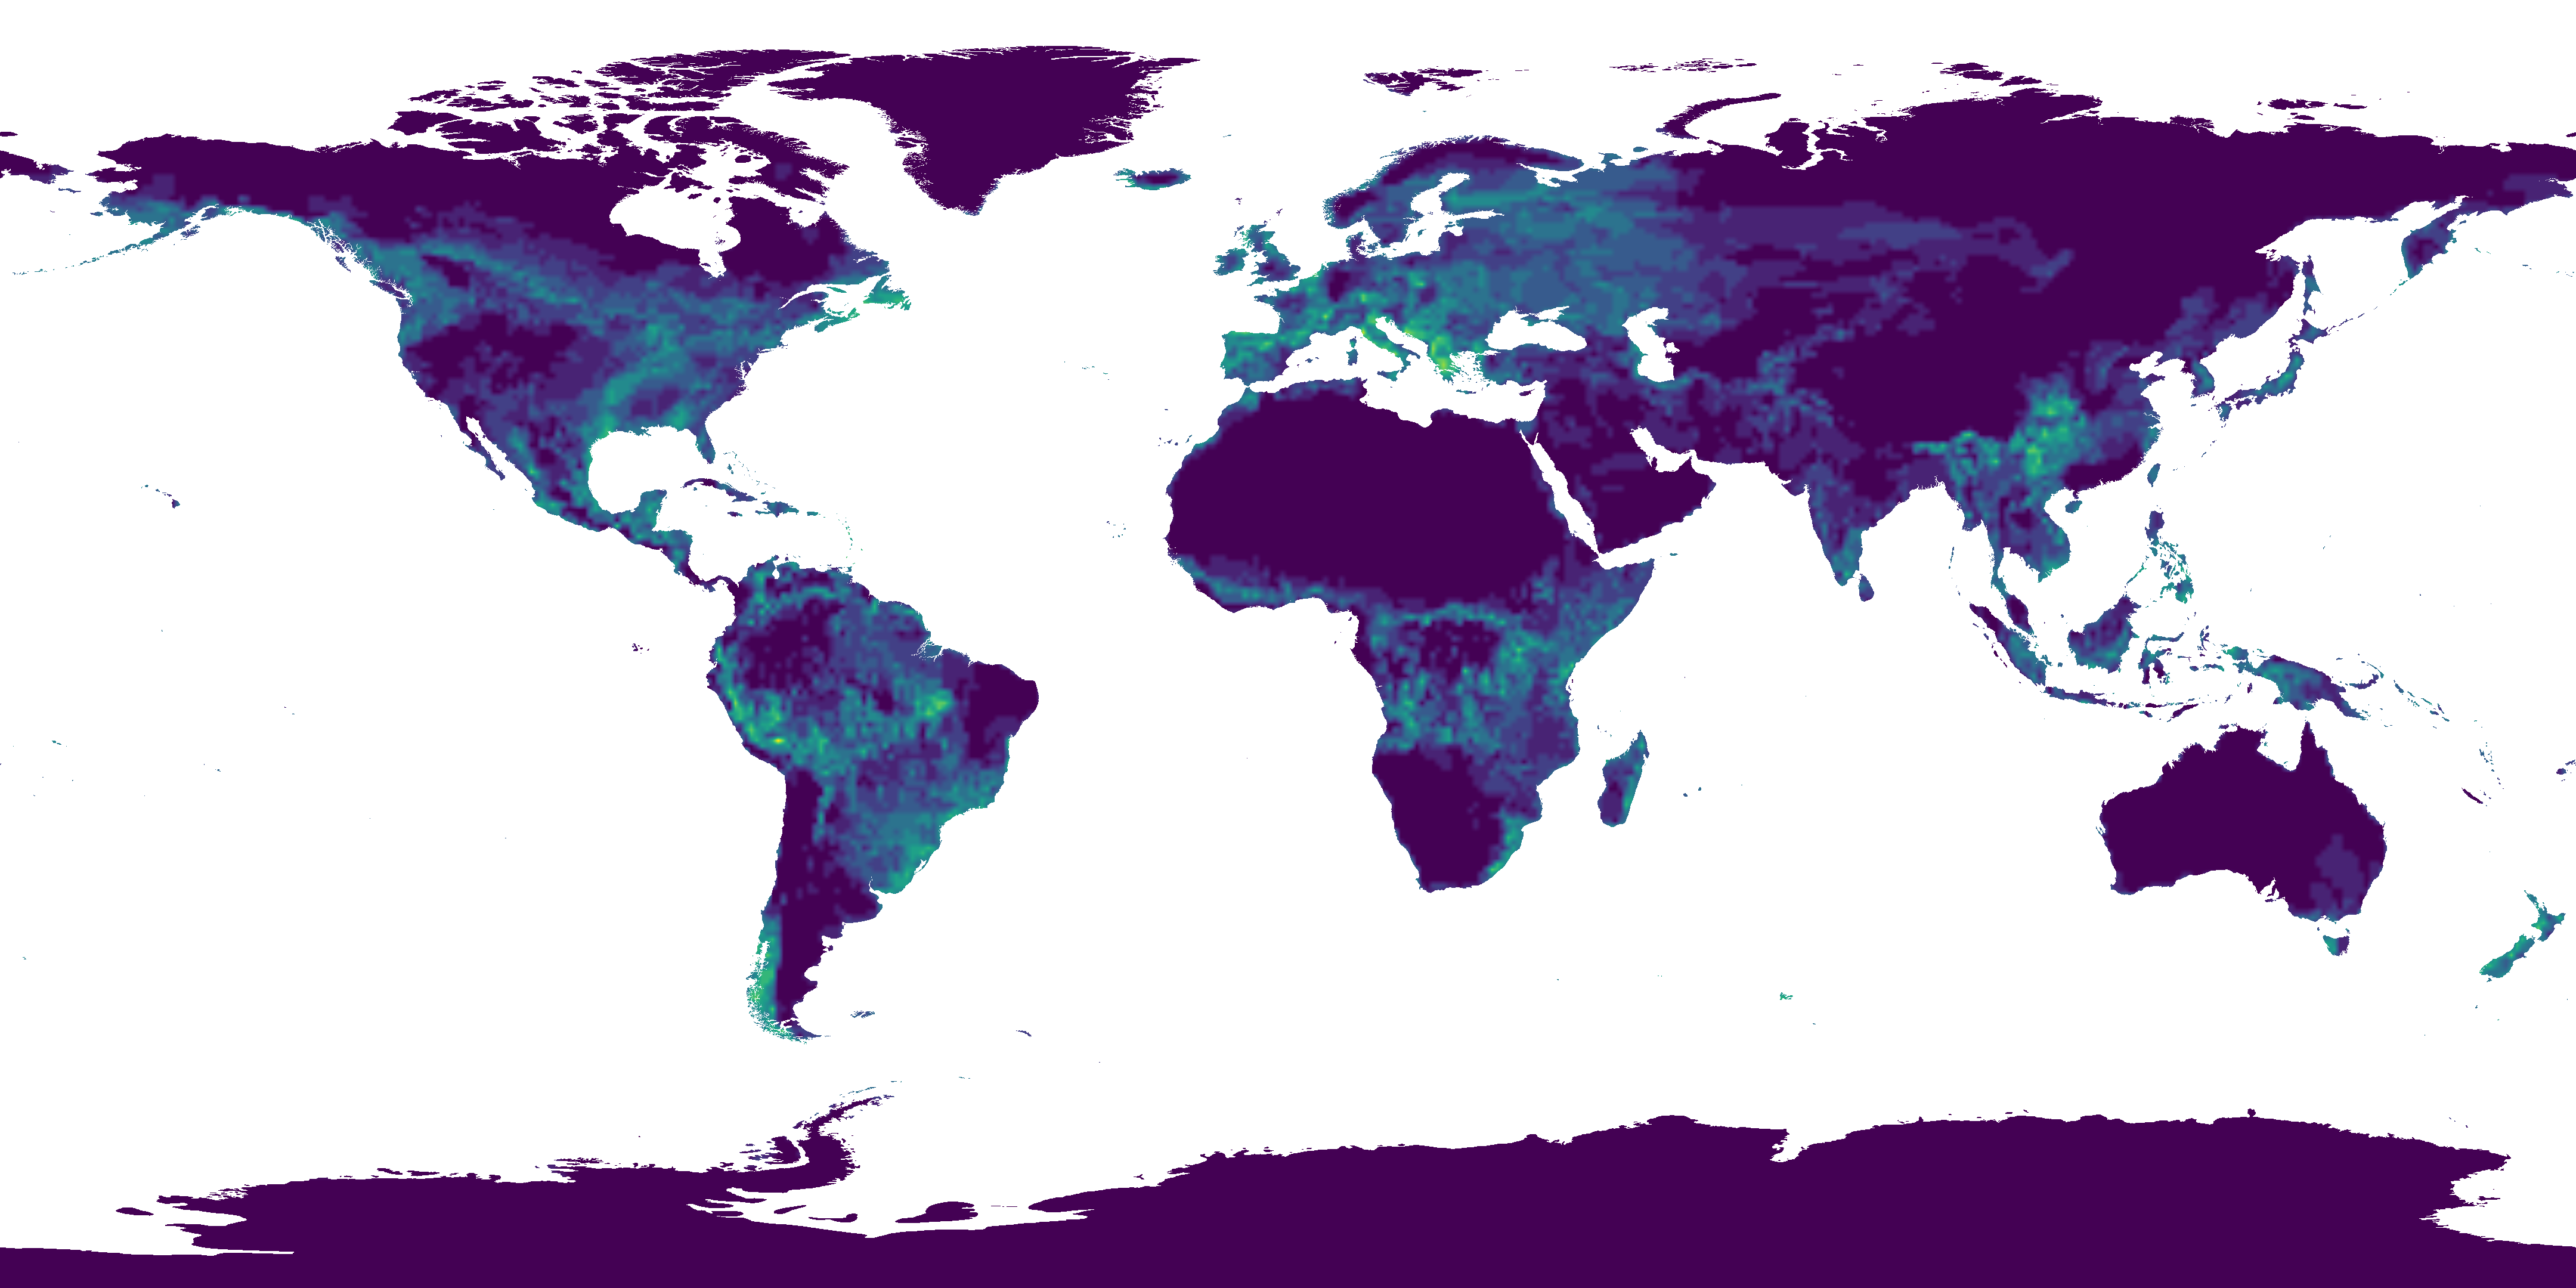
\includegraphics[width=.28\textwidth,height=2cm]{TOW_frequency_2019_11_cropped_rescaled_752b64d6_6153_498c_a86c_6dcb88a74be2.png}}\hfill
\subfloat[TOW December]{\label{sfig:f}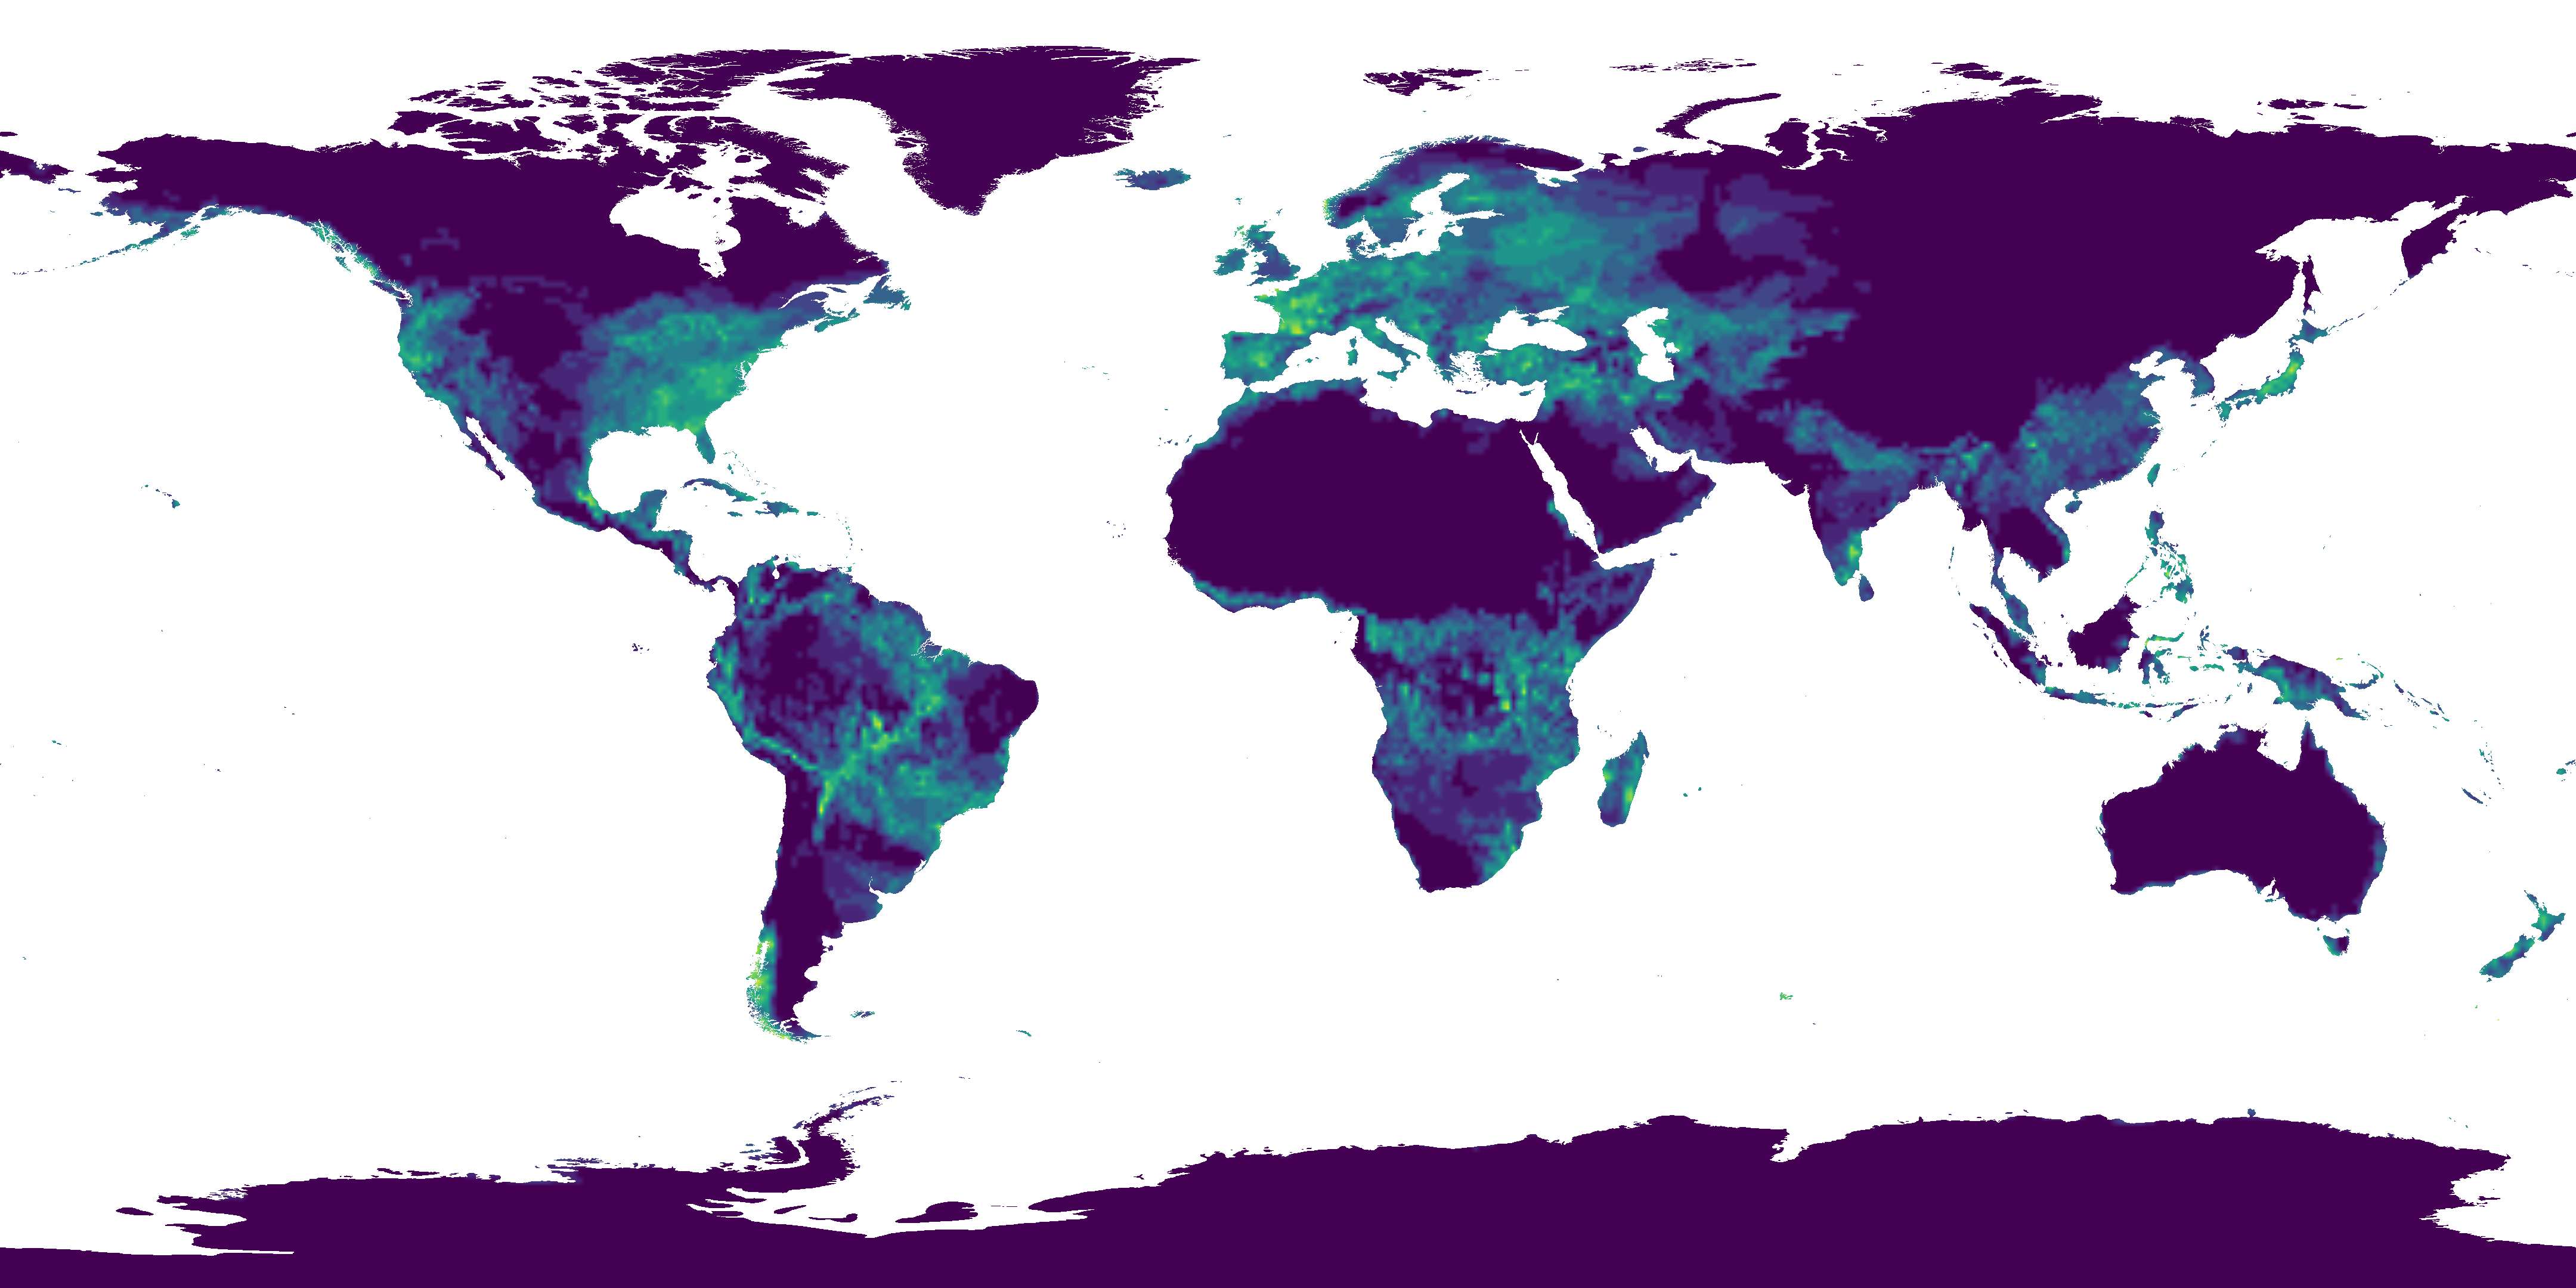
\includegraphics[width=.28\textwidth,height=2cm]{TOW_frequency_2019_12_cropped_rescaled_756c5ff5_d051_4f7f_9258_4fe3eaeb9f03.png}}\\
\caption{Time of wetness rasters for each month of the year}
\label{fig:TOW}
\end{figure}

\begin{figure}[H]
\centering
\subfloat[FOW January]{\label{sfig:a}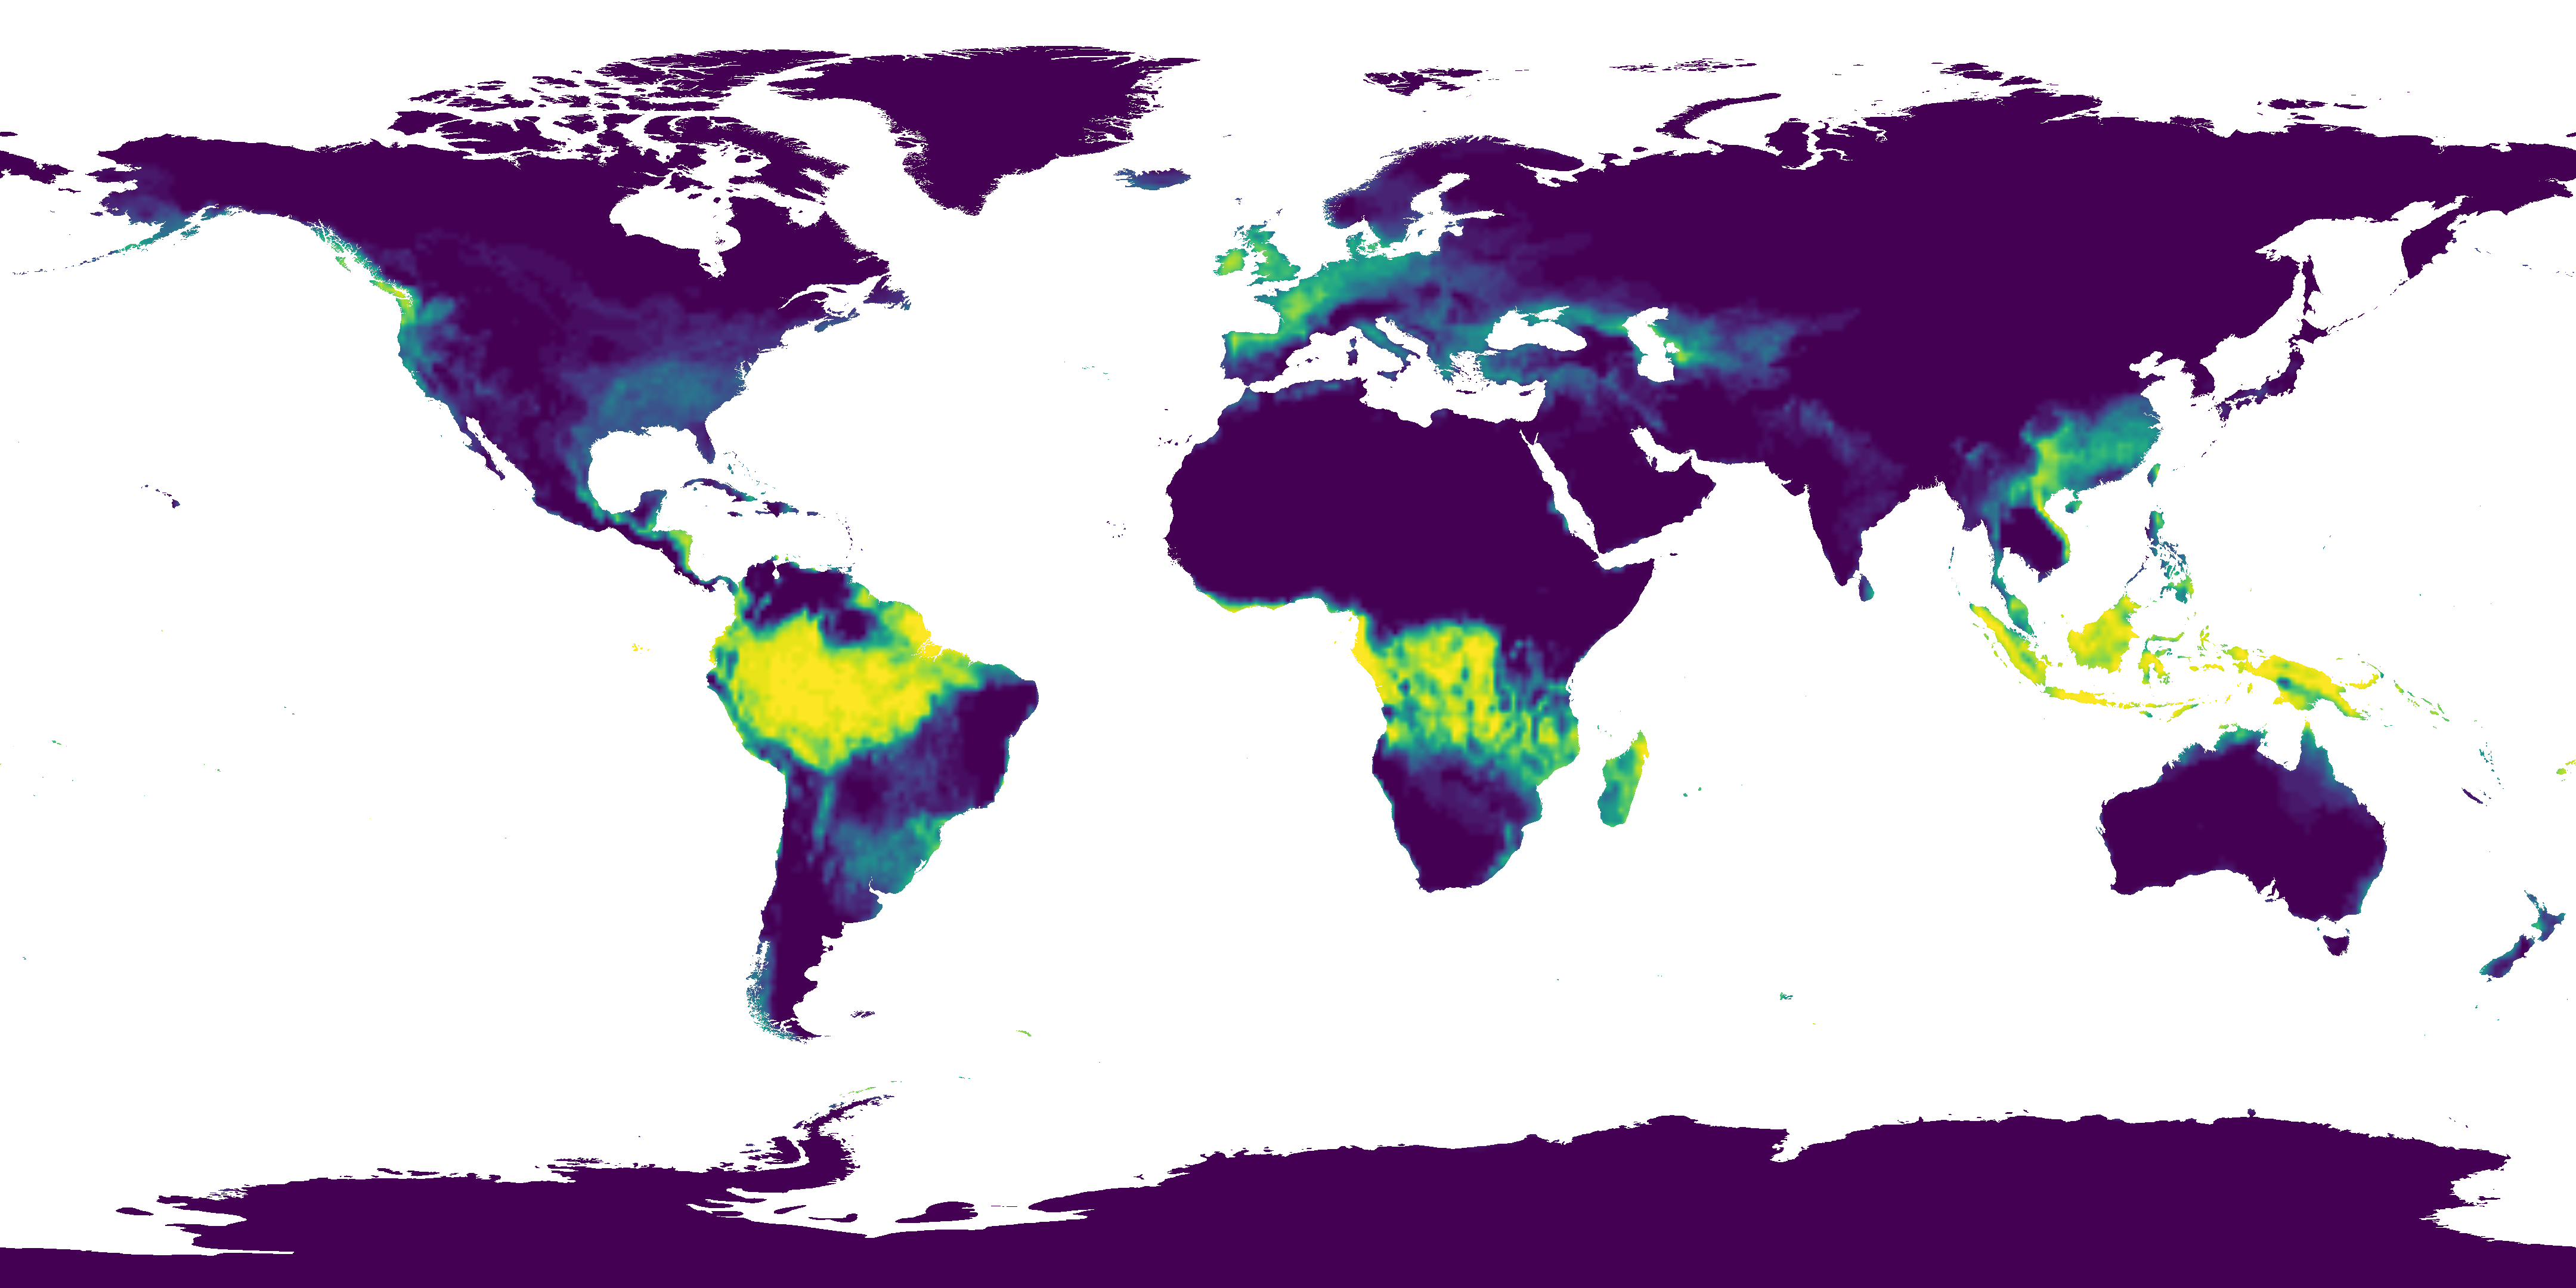
\includegraphics[width=.28\textwidth,height=2cm]{wet_monthly_2019_01_cropped_rescaled_90088c6a_a9b7_4b64_ac52_5ad858f1aa78.png}}\hfill
\subfloat[FOW February]{\label{sfig:b}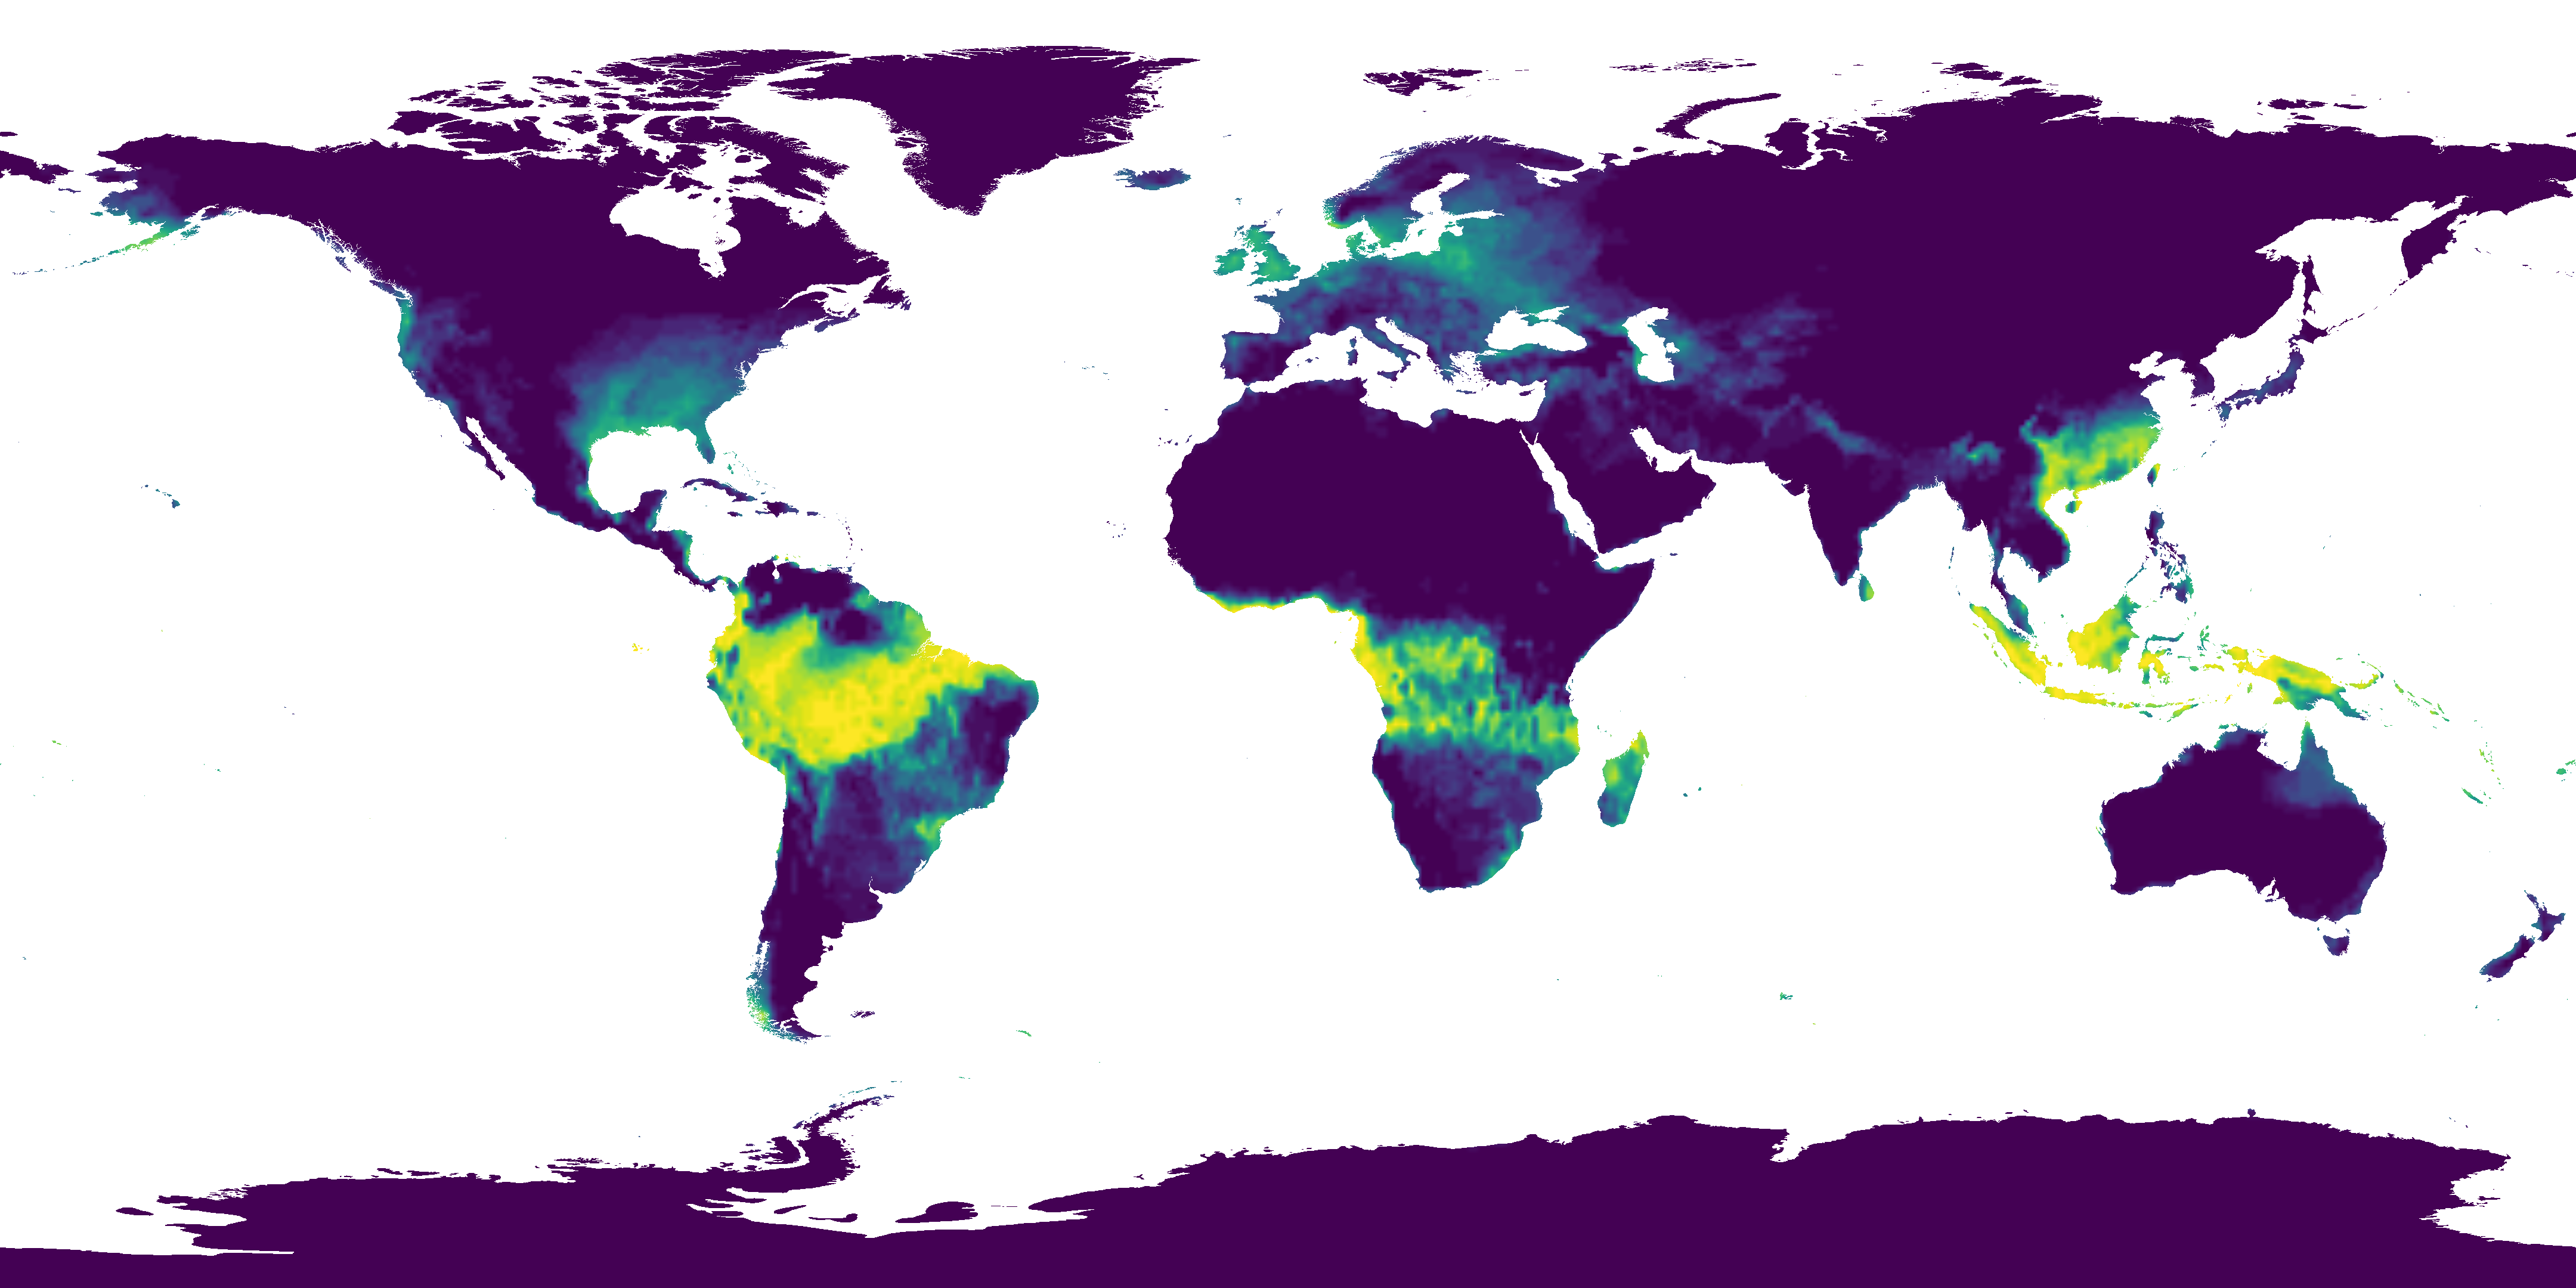
\includegraphics[width=.28\textwidth,height=2cm]{wet_monthly_2019_02_cropped_rescaled_6f45c01d_d28b_46f1_b90b_e827e0b61e55.png}}\hfill
\subfloat[FOW March]{\label{sfig:c}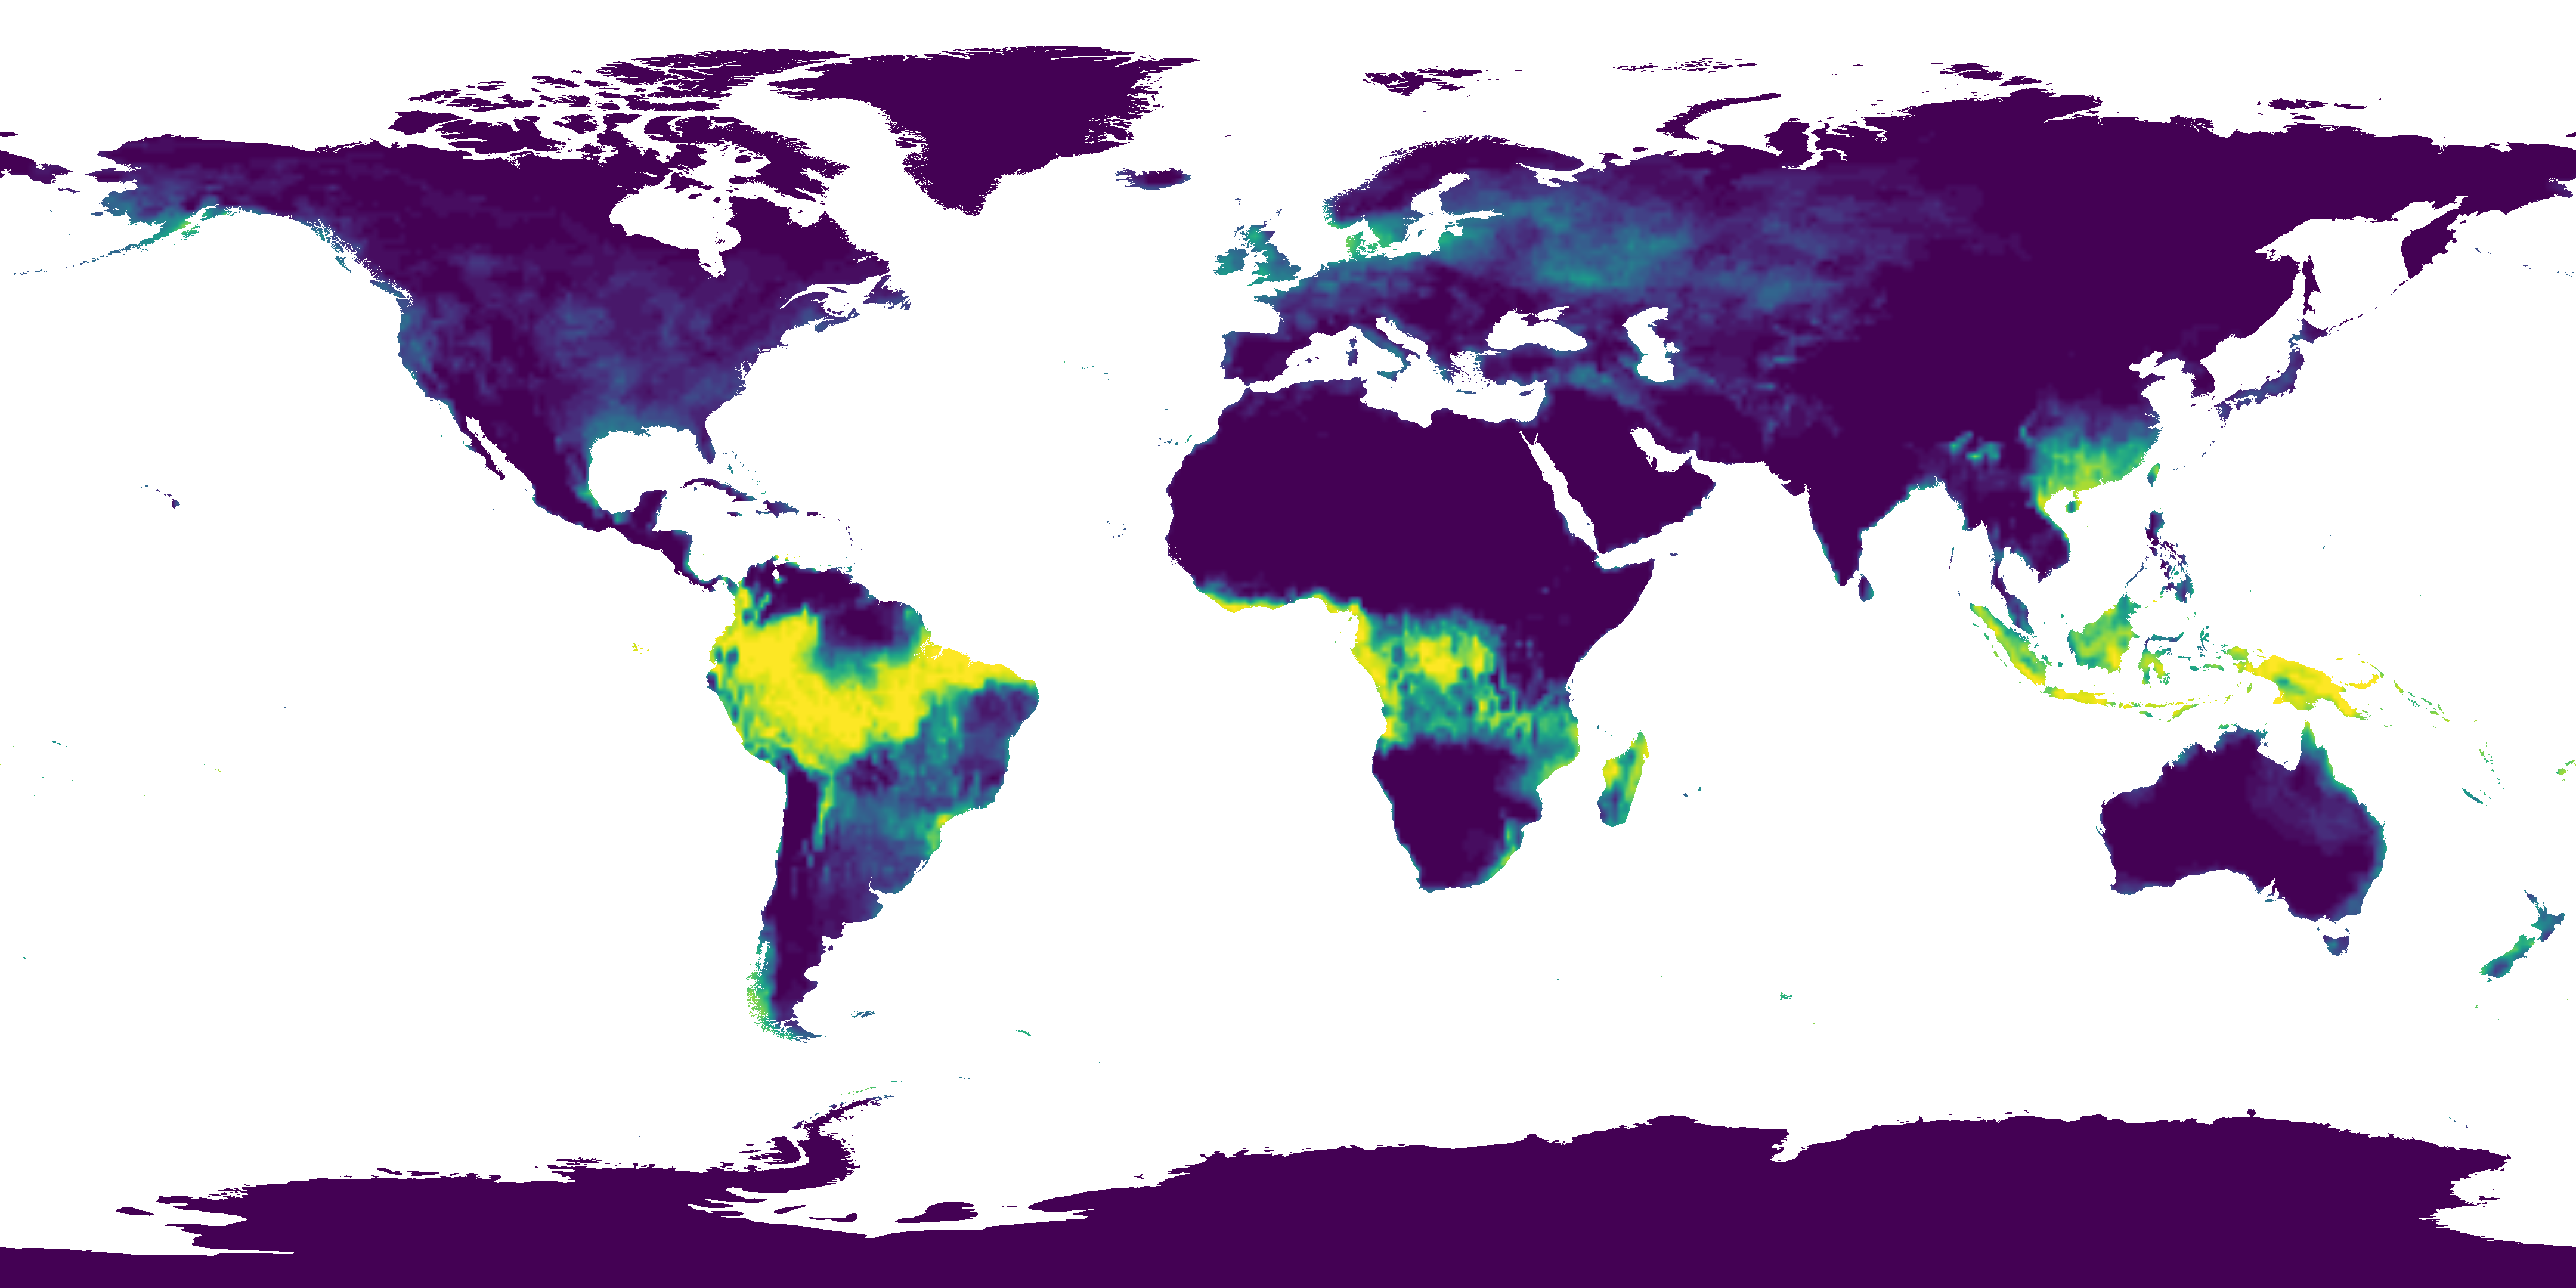
\includegraphics[width=.28\textwidth,height=2cm]{wet_monthly_2019_03_cropped_rescaled_f516b4ae_4add_4841_b186_63a7126ea65e.png}}\\
\subfloat[FOW April]{\label{sfig:d}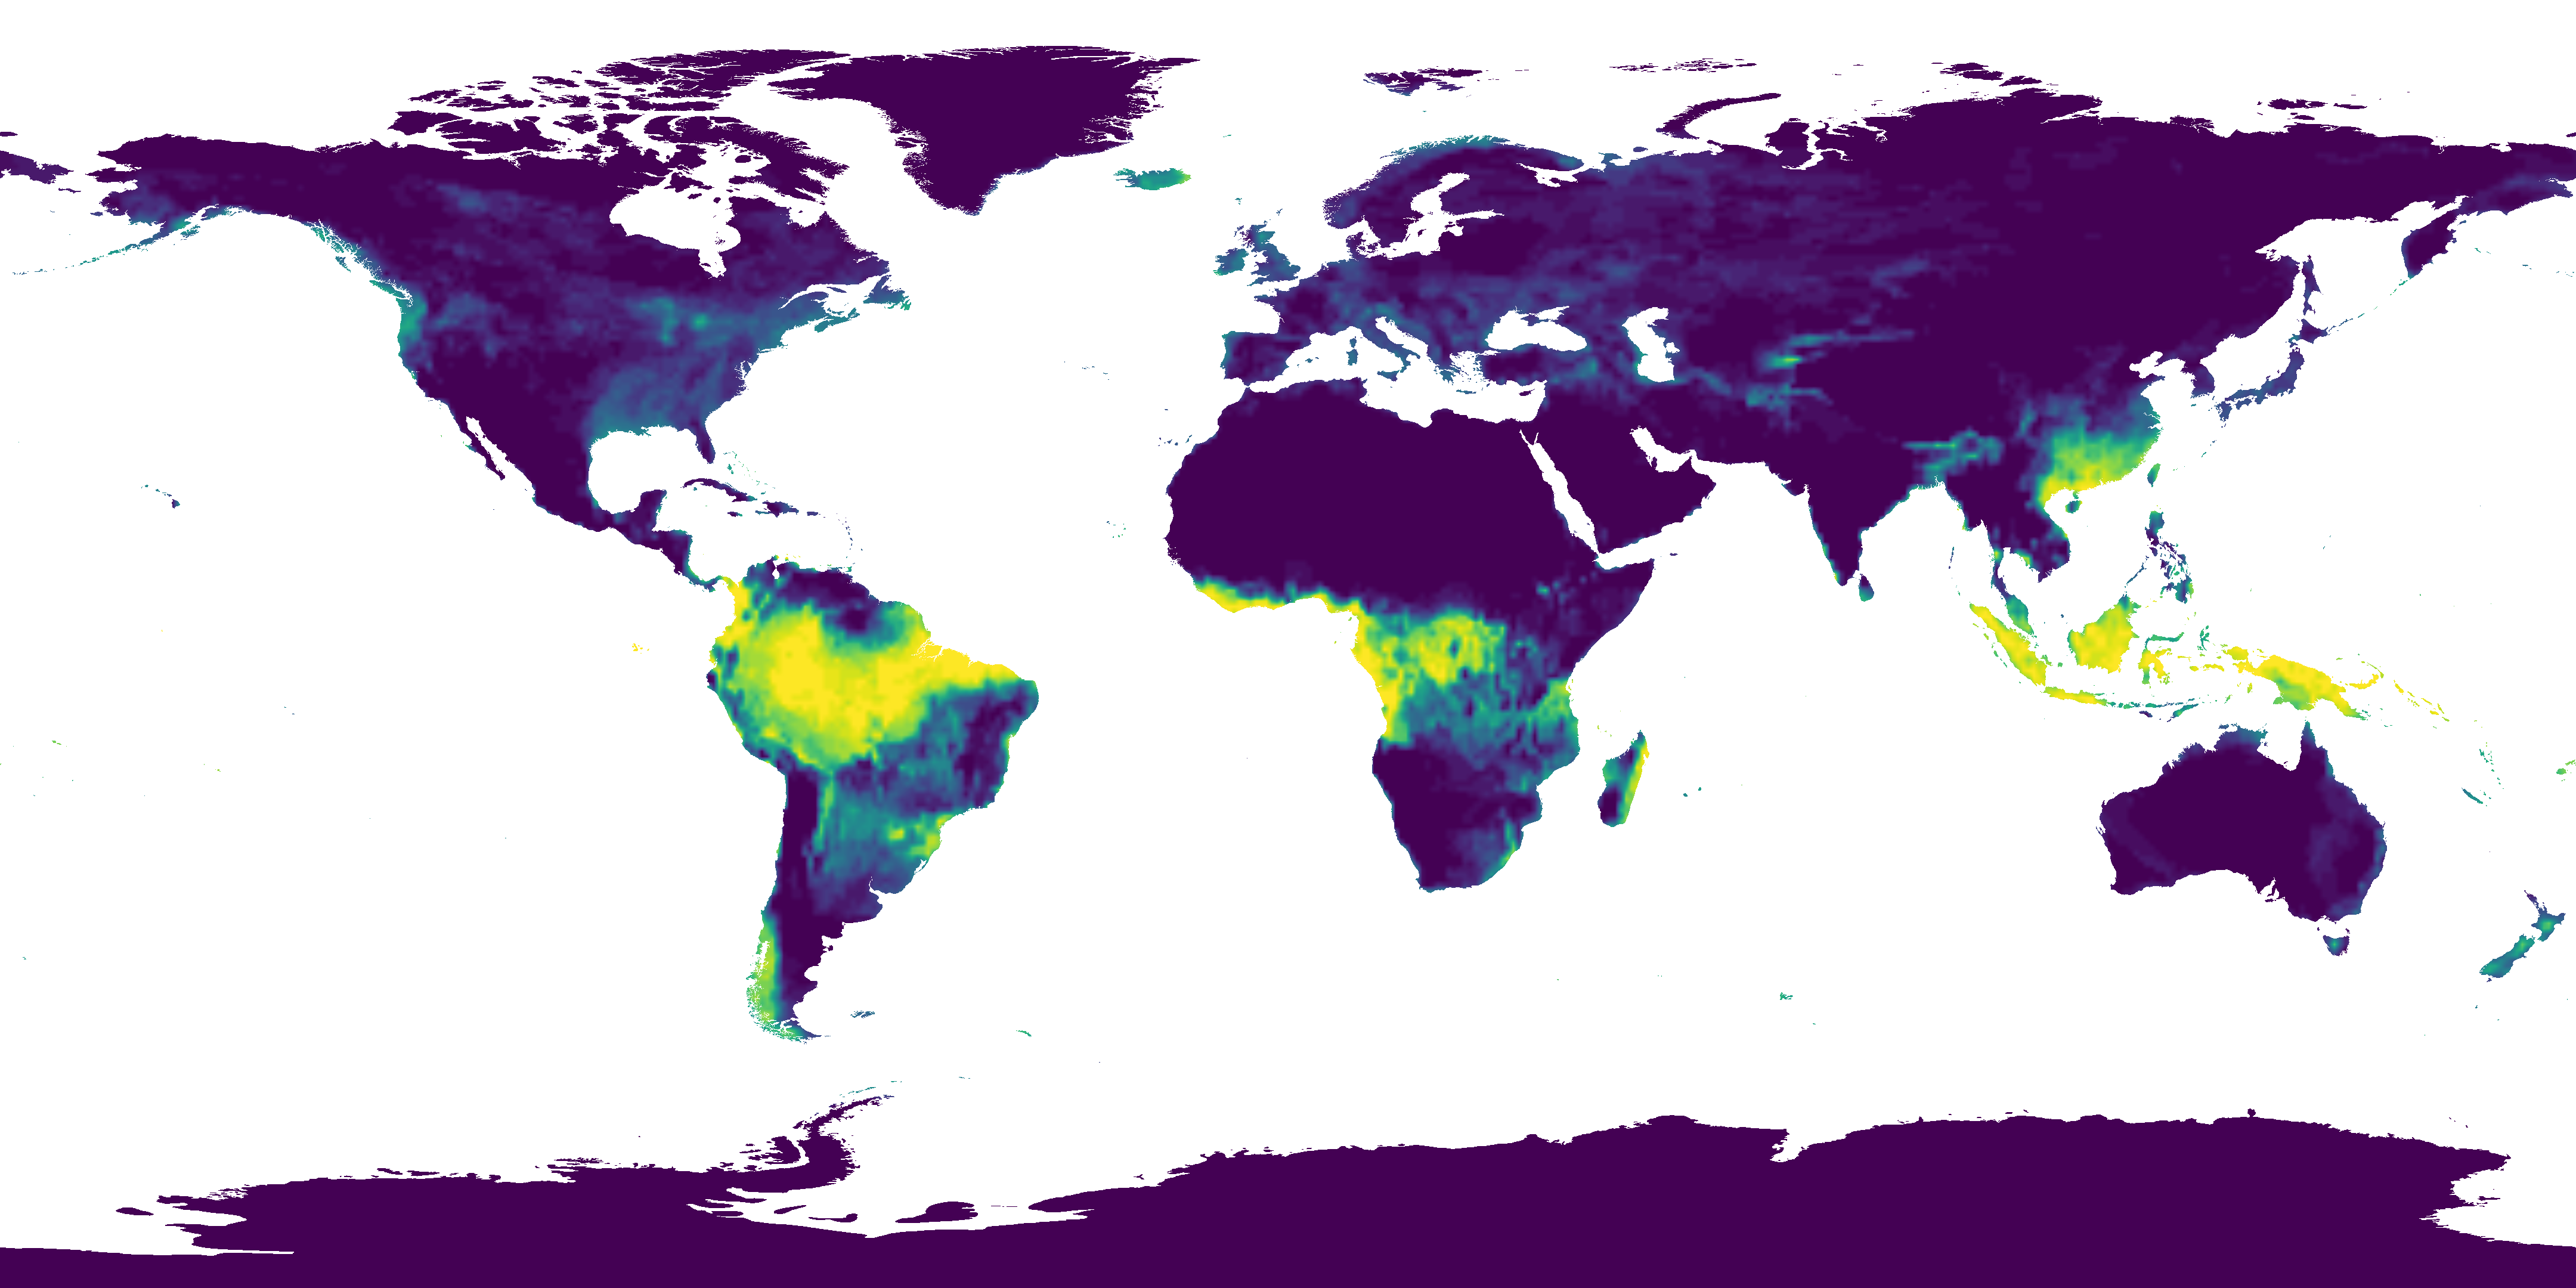
\includegraphics[width=.28\textwidth,height=2cm]{wet_monthly_2019_04_cropped_rescaled_95f9fb12_caa5_4f7c_afcd_6feb3e6b17f9.png}}\hfill
\subfloat[FOW May]{\label{sfig:e}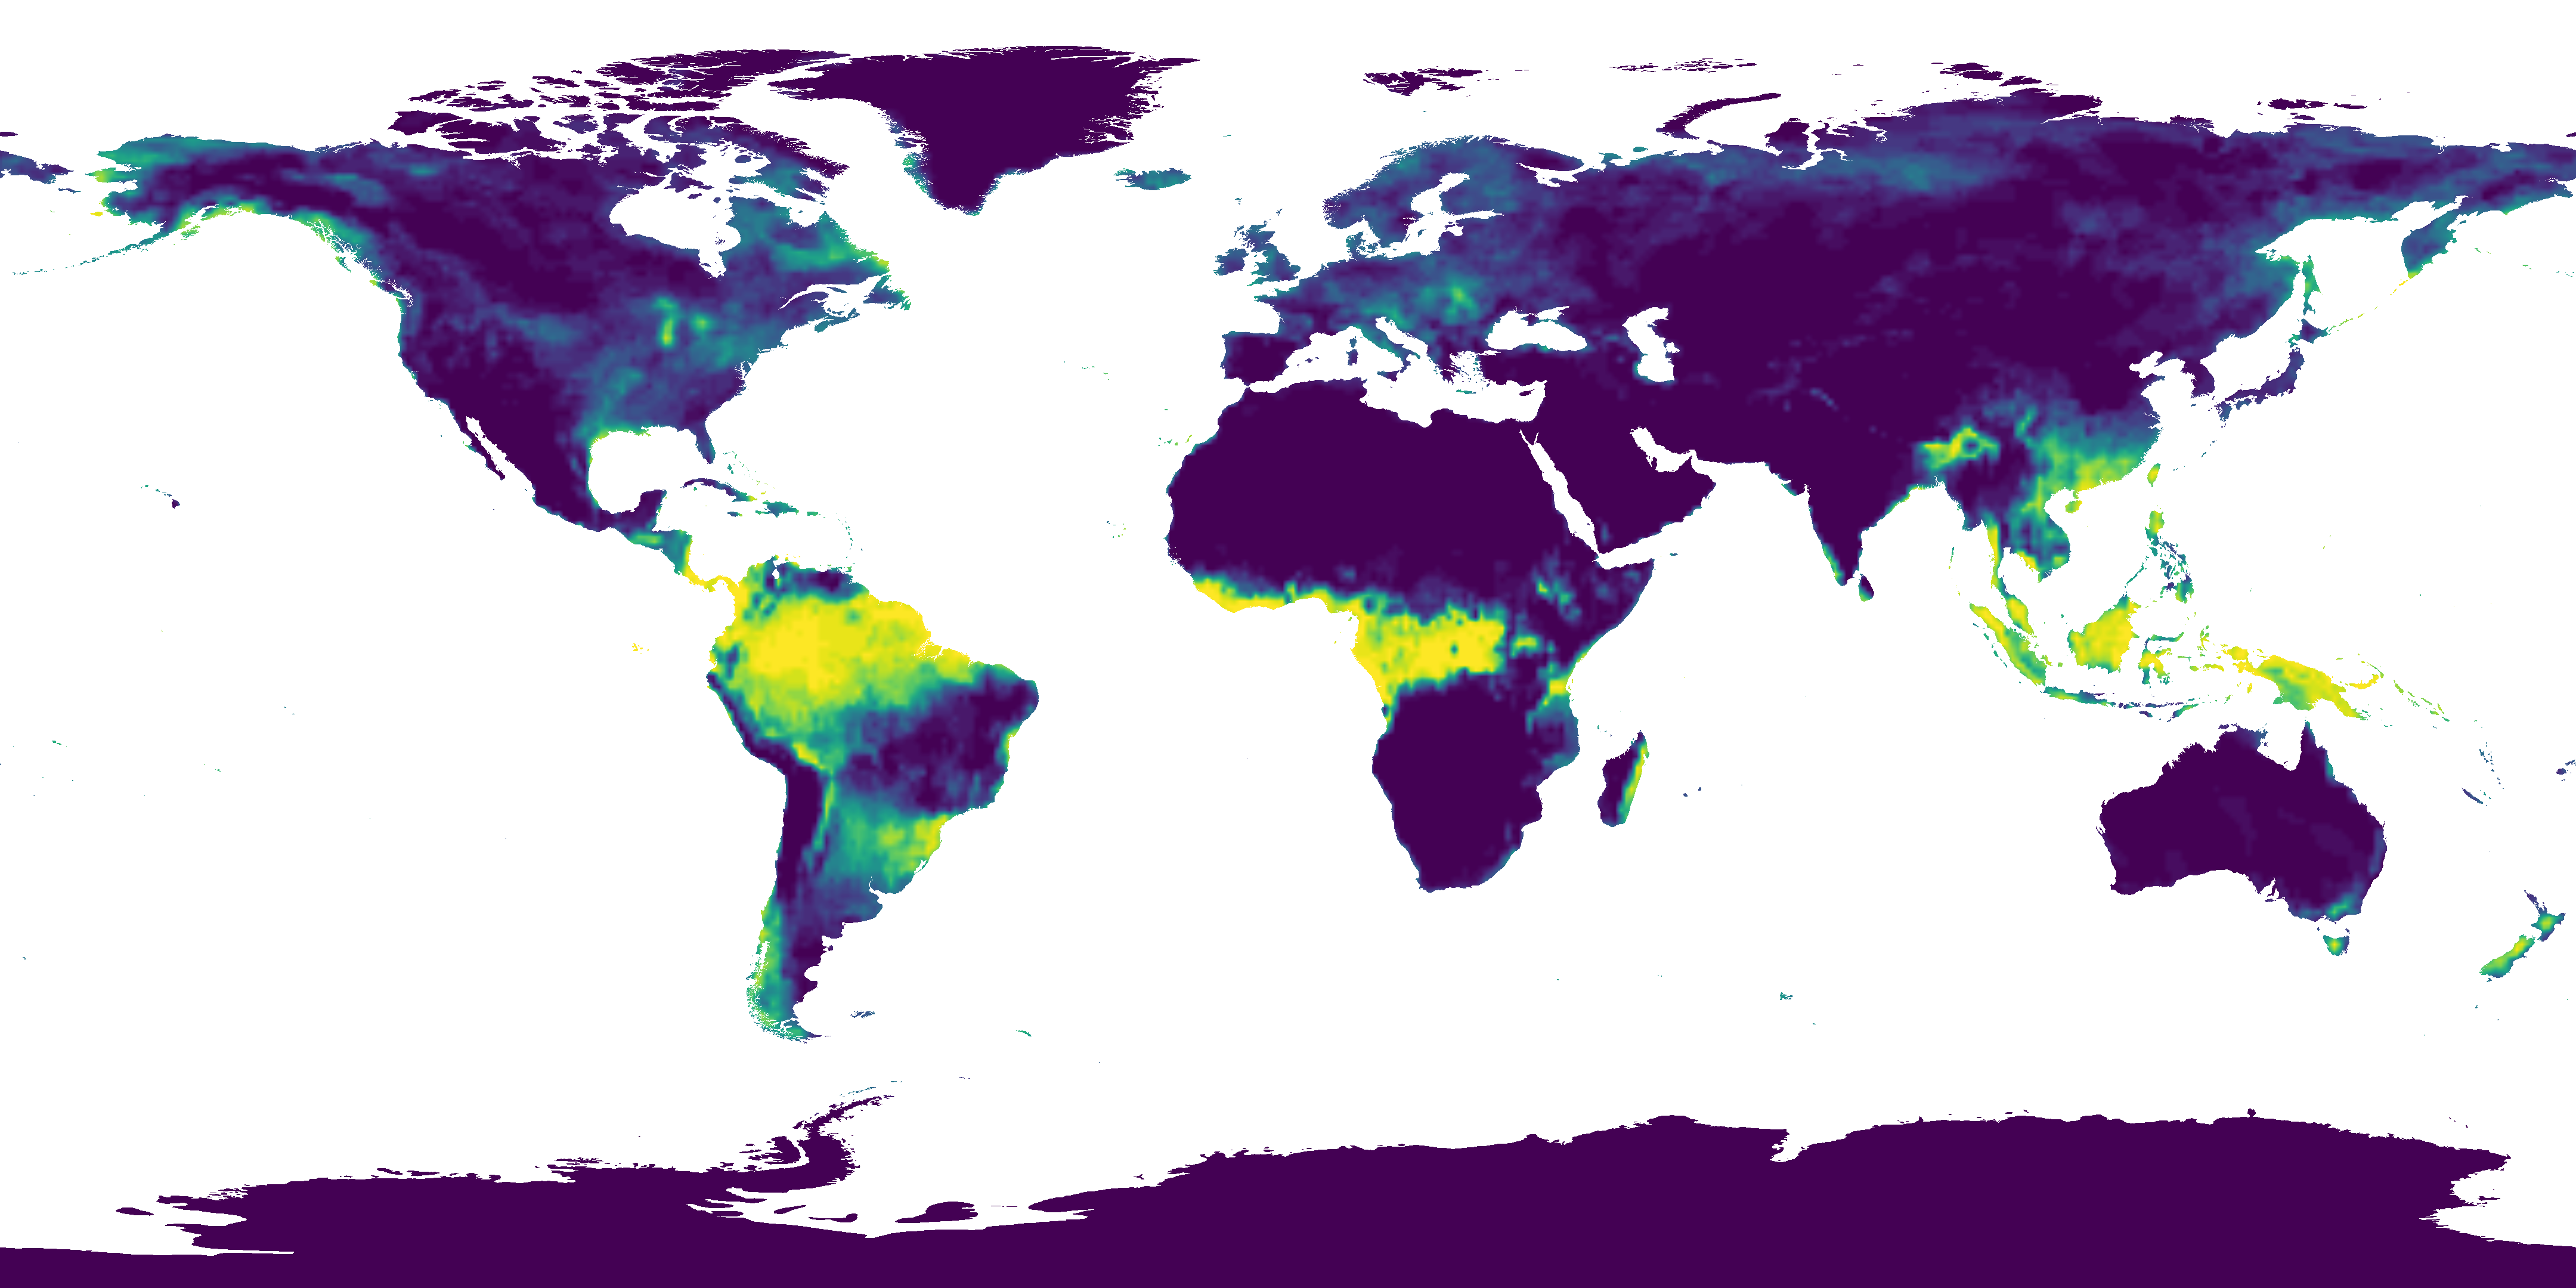
\includegraphics[width=.28\textwidth,height=2cm]{wet_monthly_2019_05_cropped_rescaled_cc61b3d9_9216_4ac8_83bb_aba453309f55.png}}\hfill
\subfloat[FOW June]{\label{sfig:f}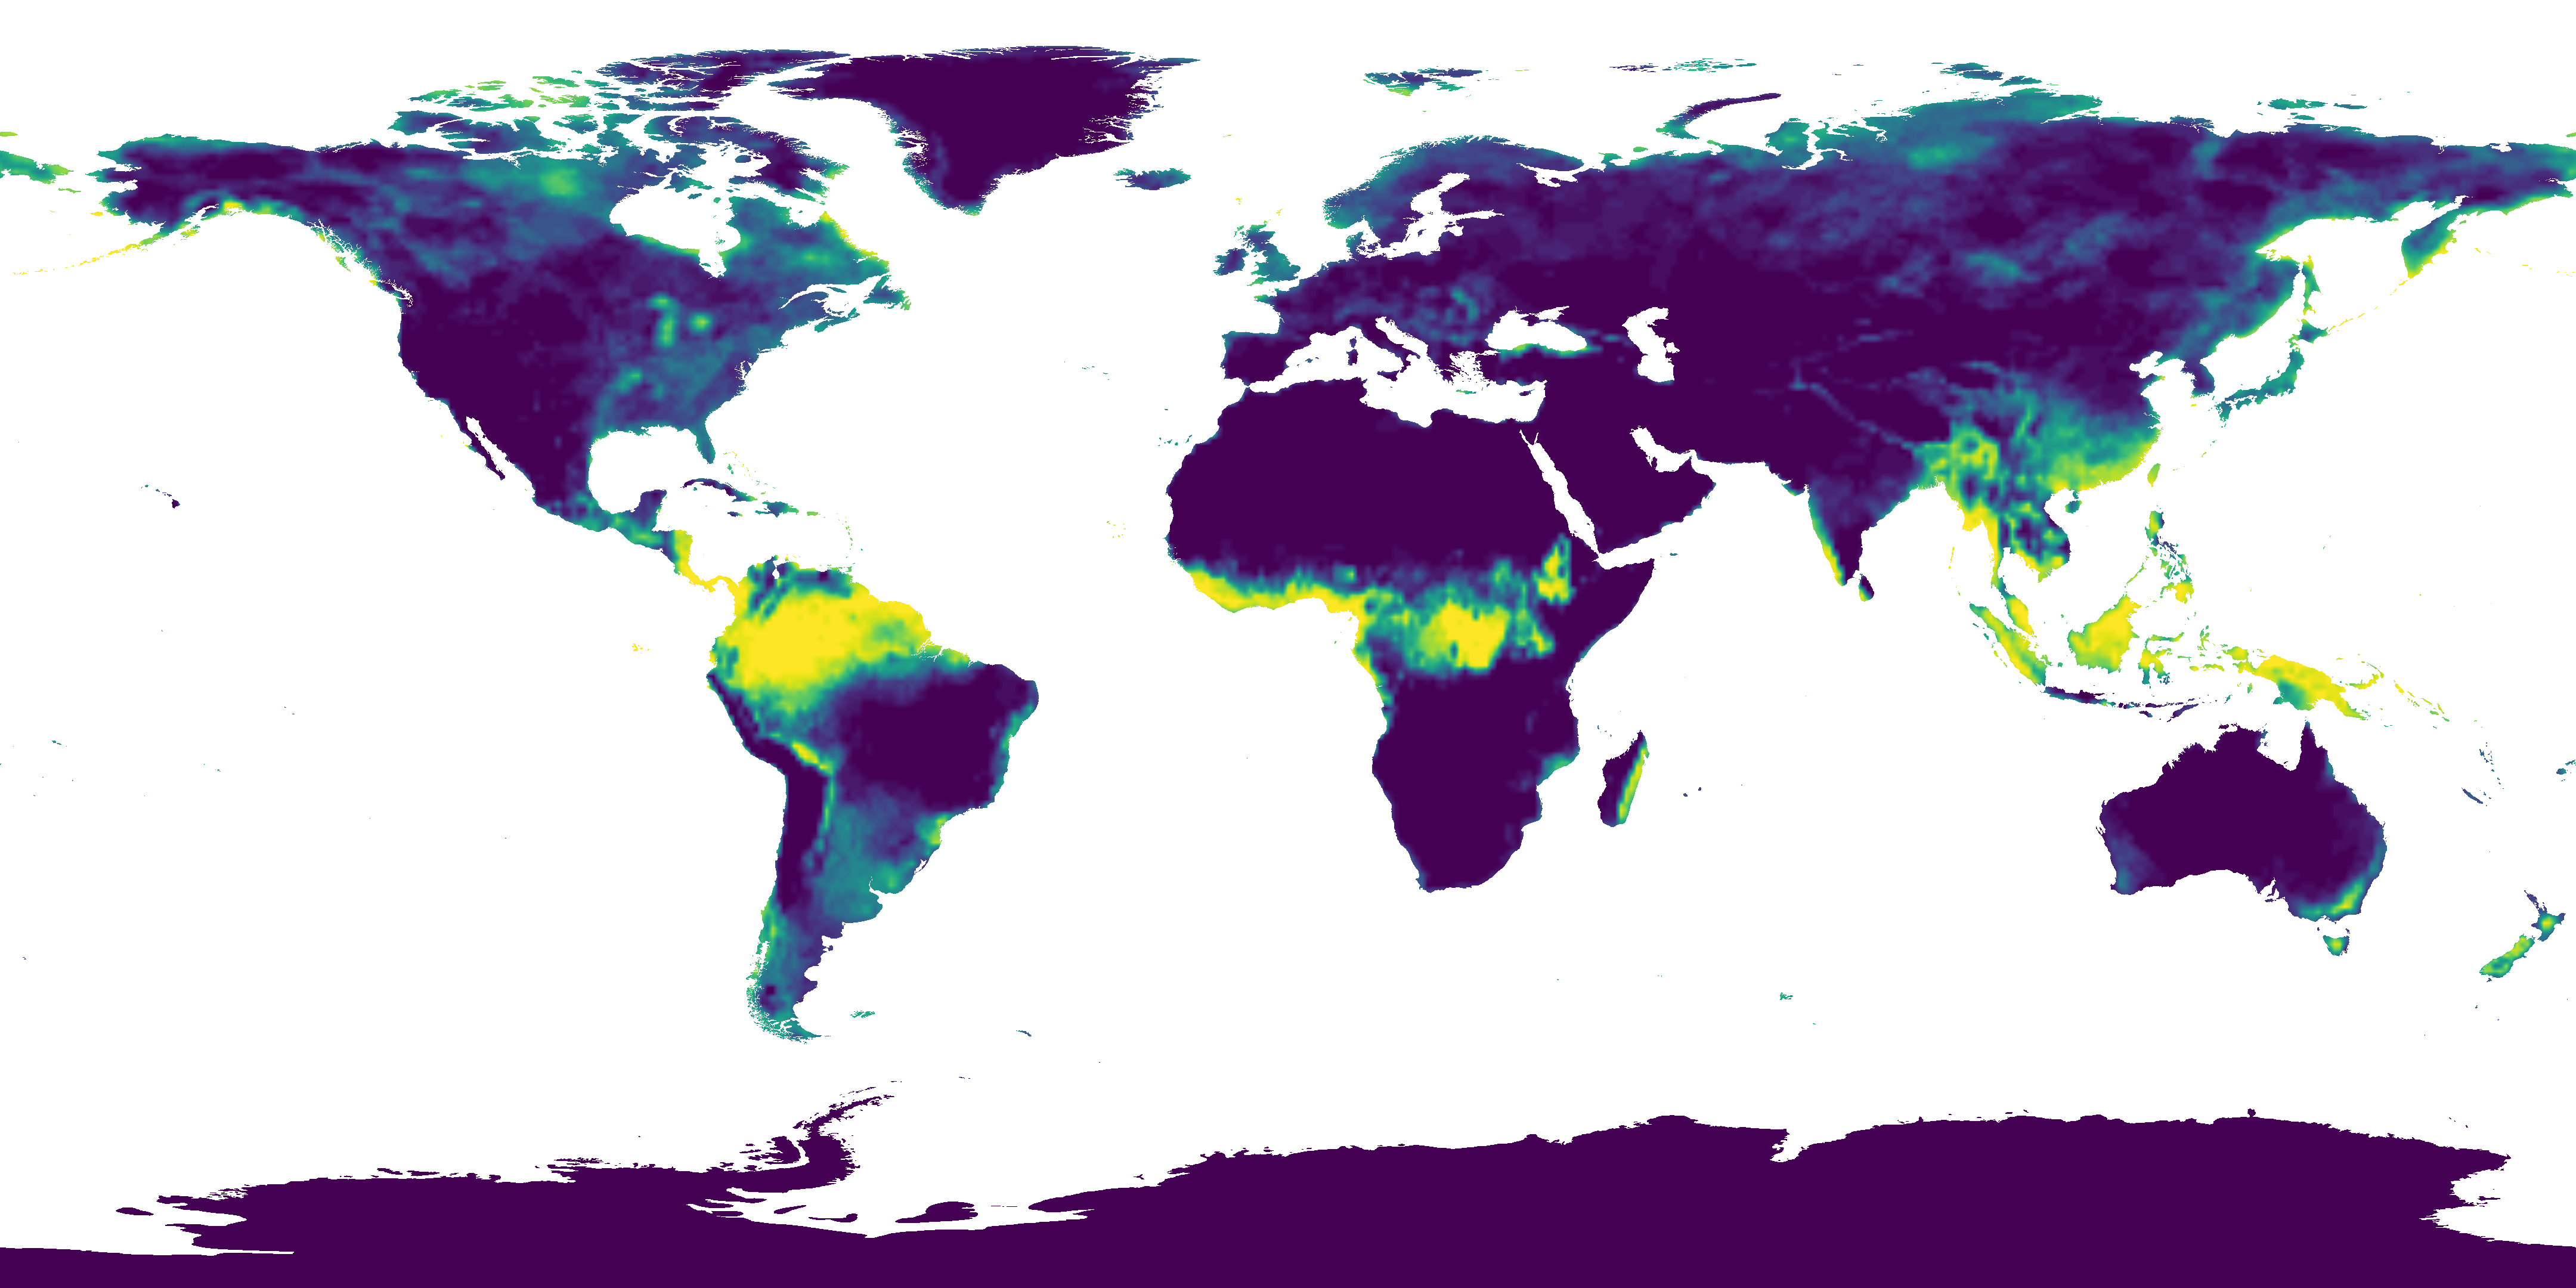
\includegraphics[width=.28\textwidth,height=2cm]{wet_monthly_2019_06_cropped_rescaled_9dc8b582_721d_48ba_a0b8_62b389d2ea61.png}}\\
\subfloat[FOW July]{\label{sfig:a}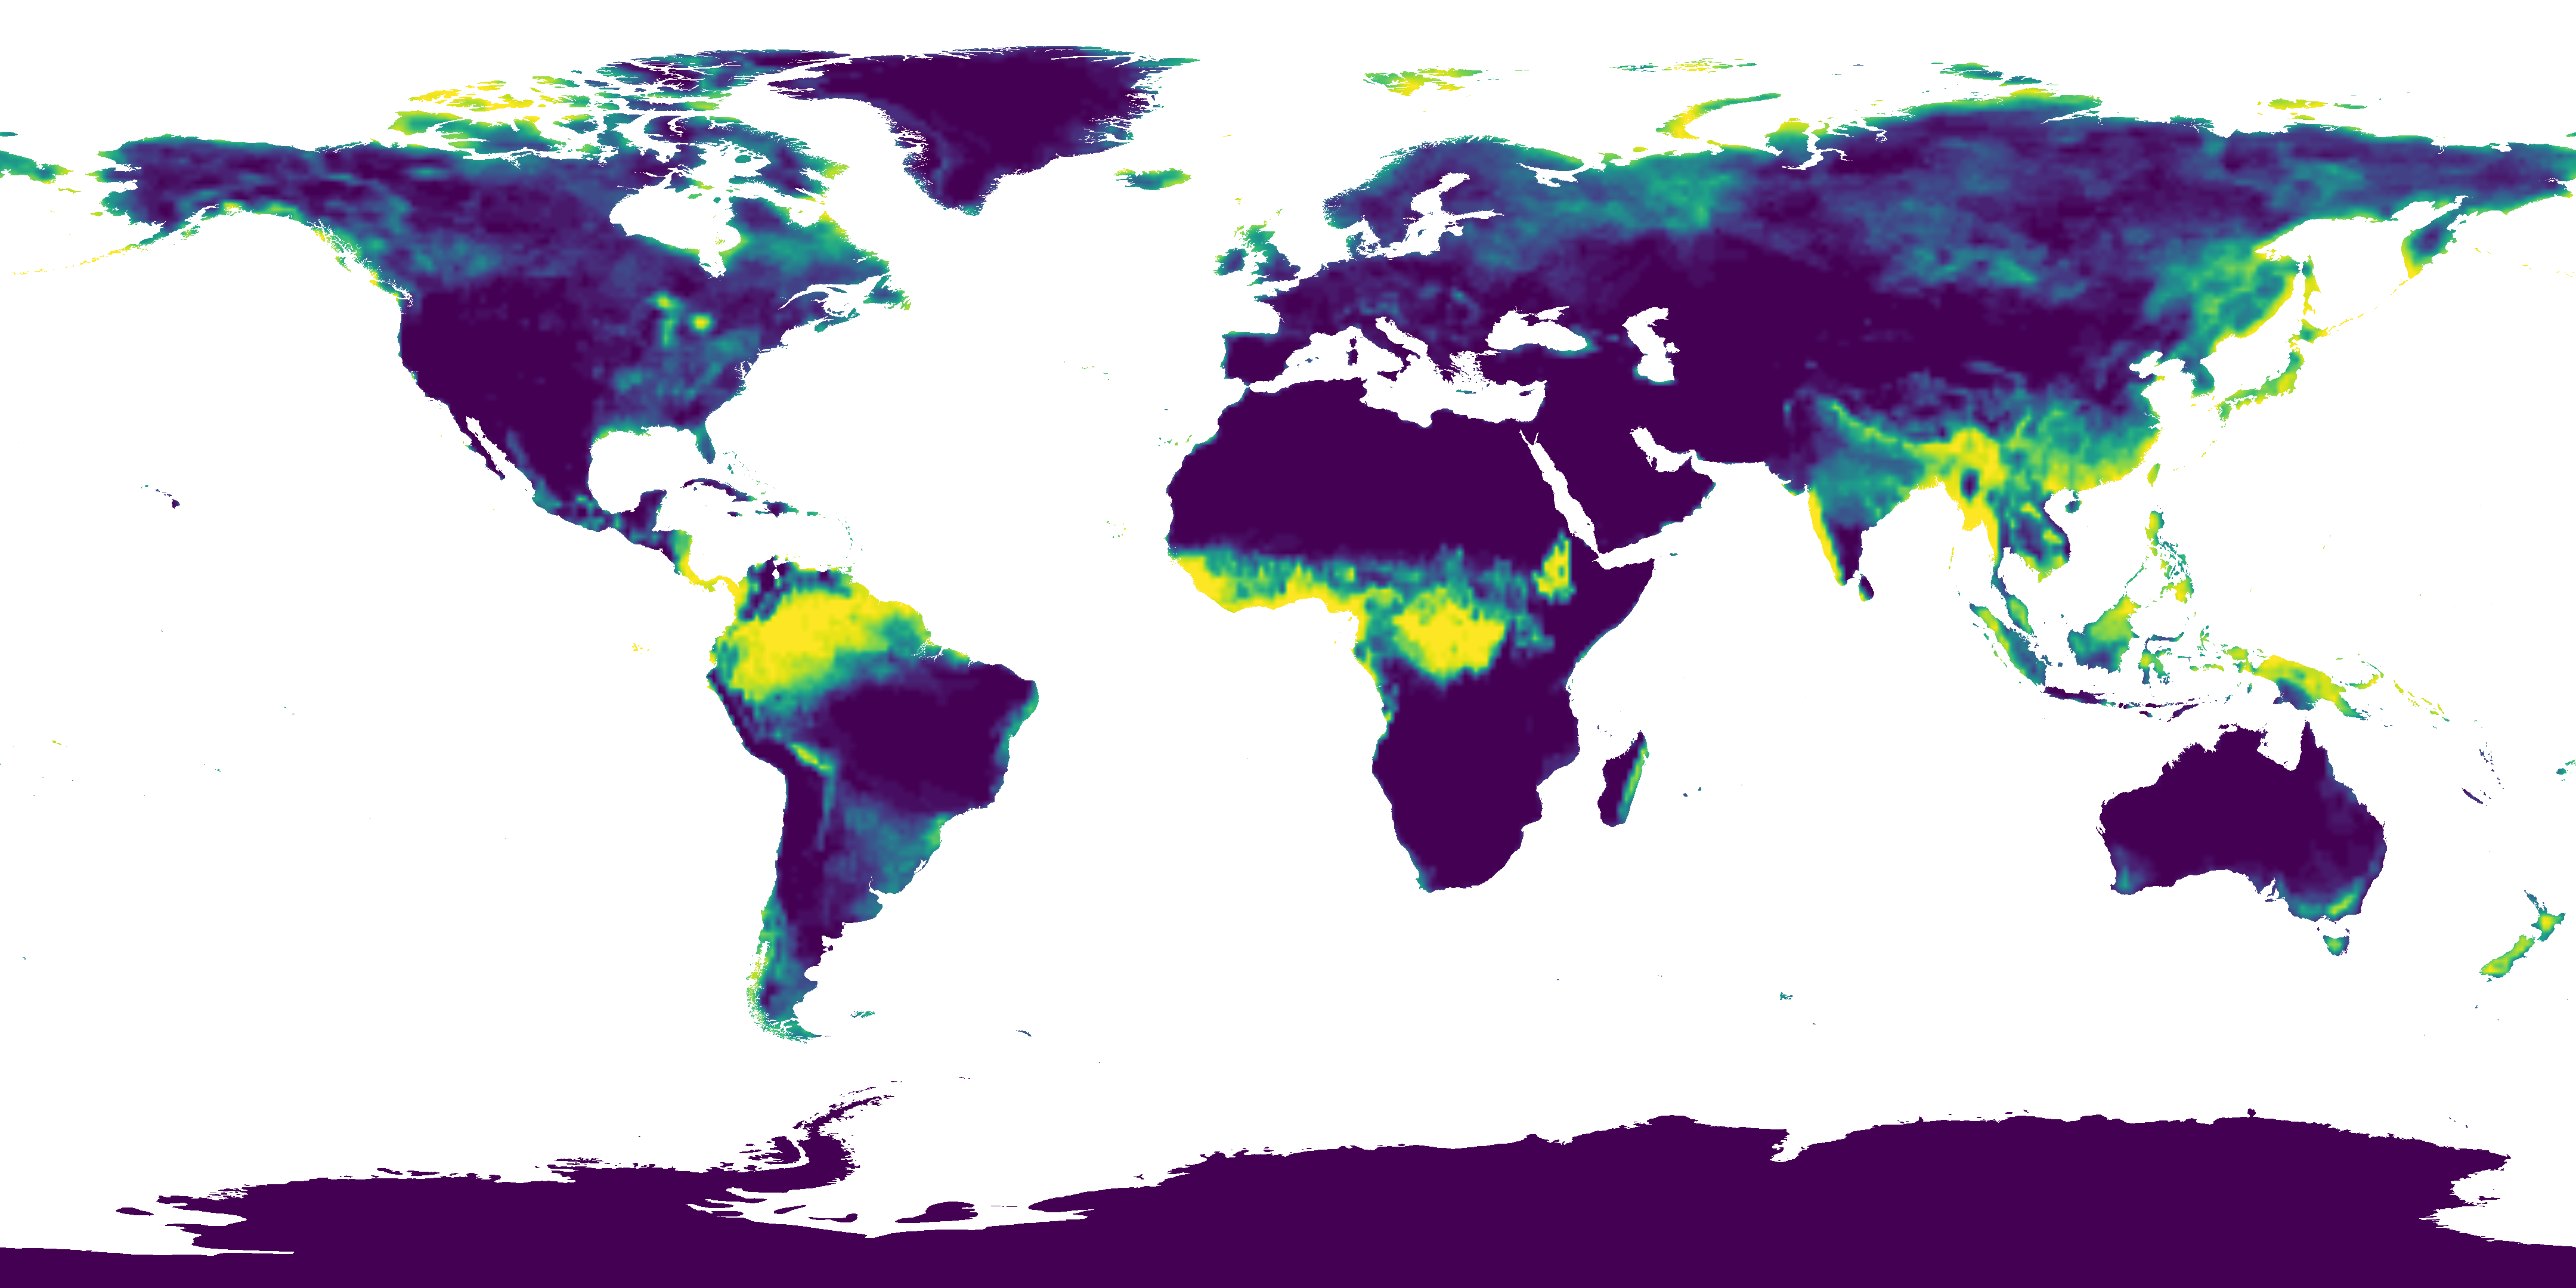
\includegraphics[width=.28\textwidth,height=2cm]{wet_monthly_2019_07_cropped_rescaled_5633890d_bac5_49b6_88b6_dca35f64e743.png}}\hfill
\subfloat[FOW August]{\label{sfig:b}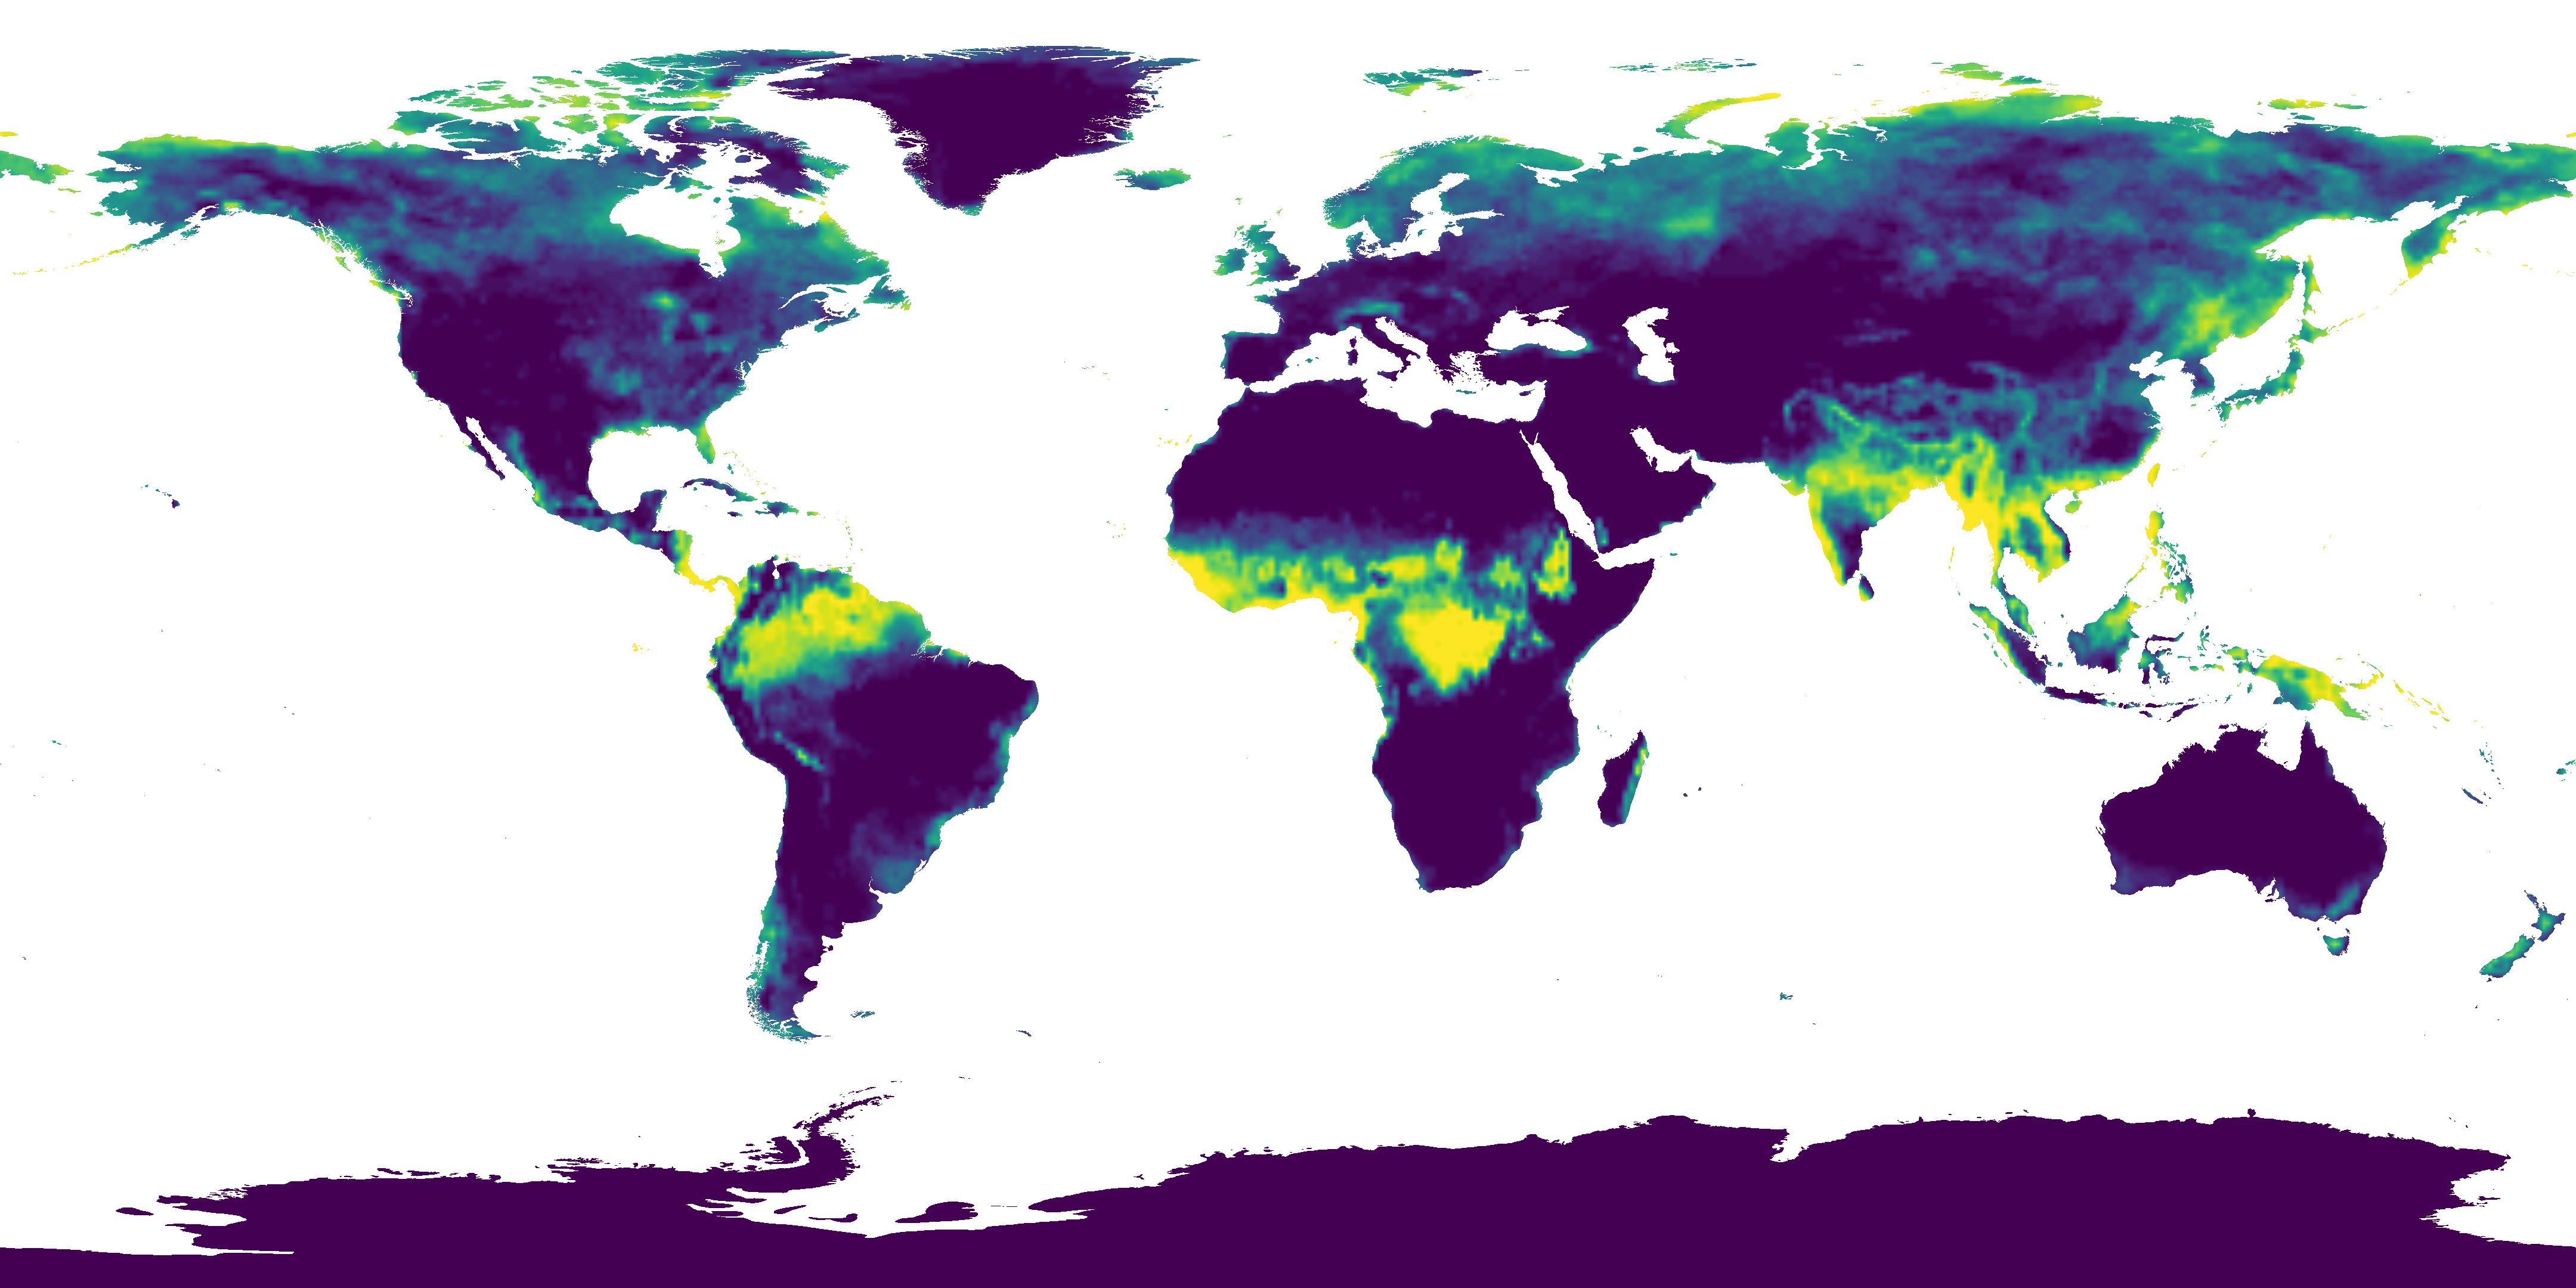
\includegraphics[width=.28\textwidth,height=2cm]{wet_monthly_2019_08_cropped_rescaled_6c66a1f8_9f55_4e88_8b34_a4c6254b8fde.png}}\hfill
\subfloat[FOW September]{\label{sfig:c}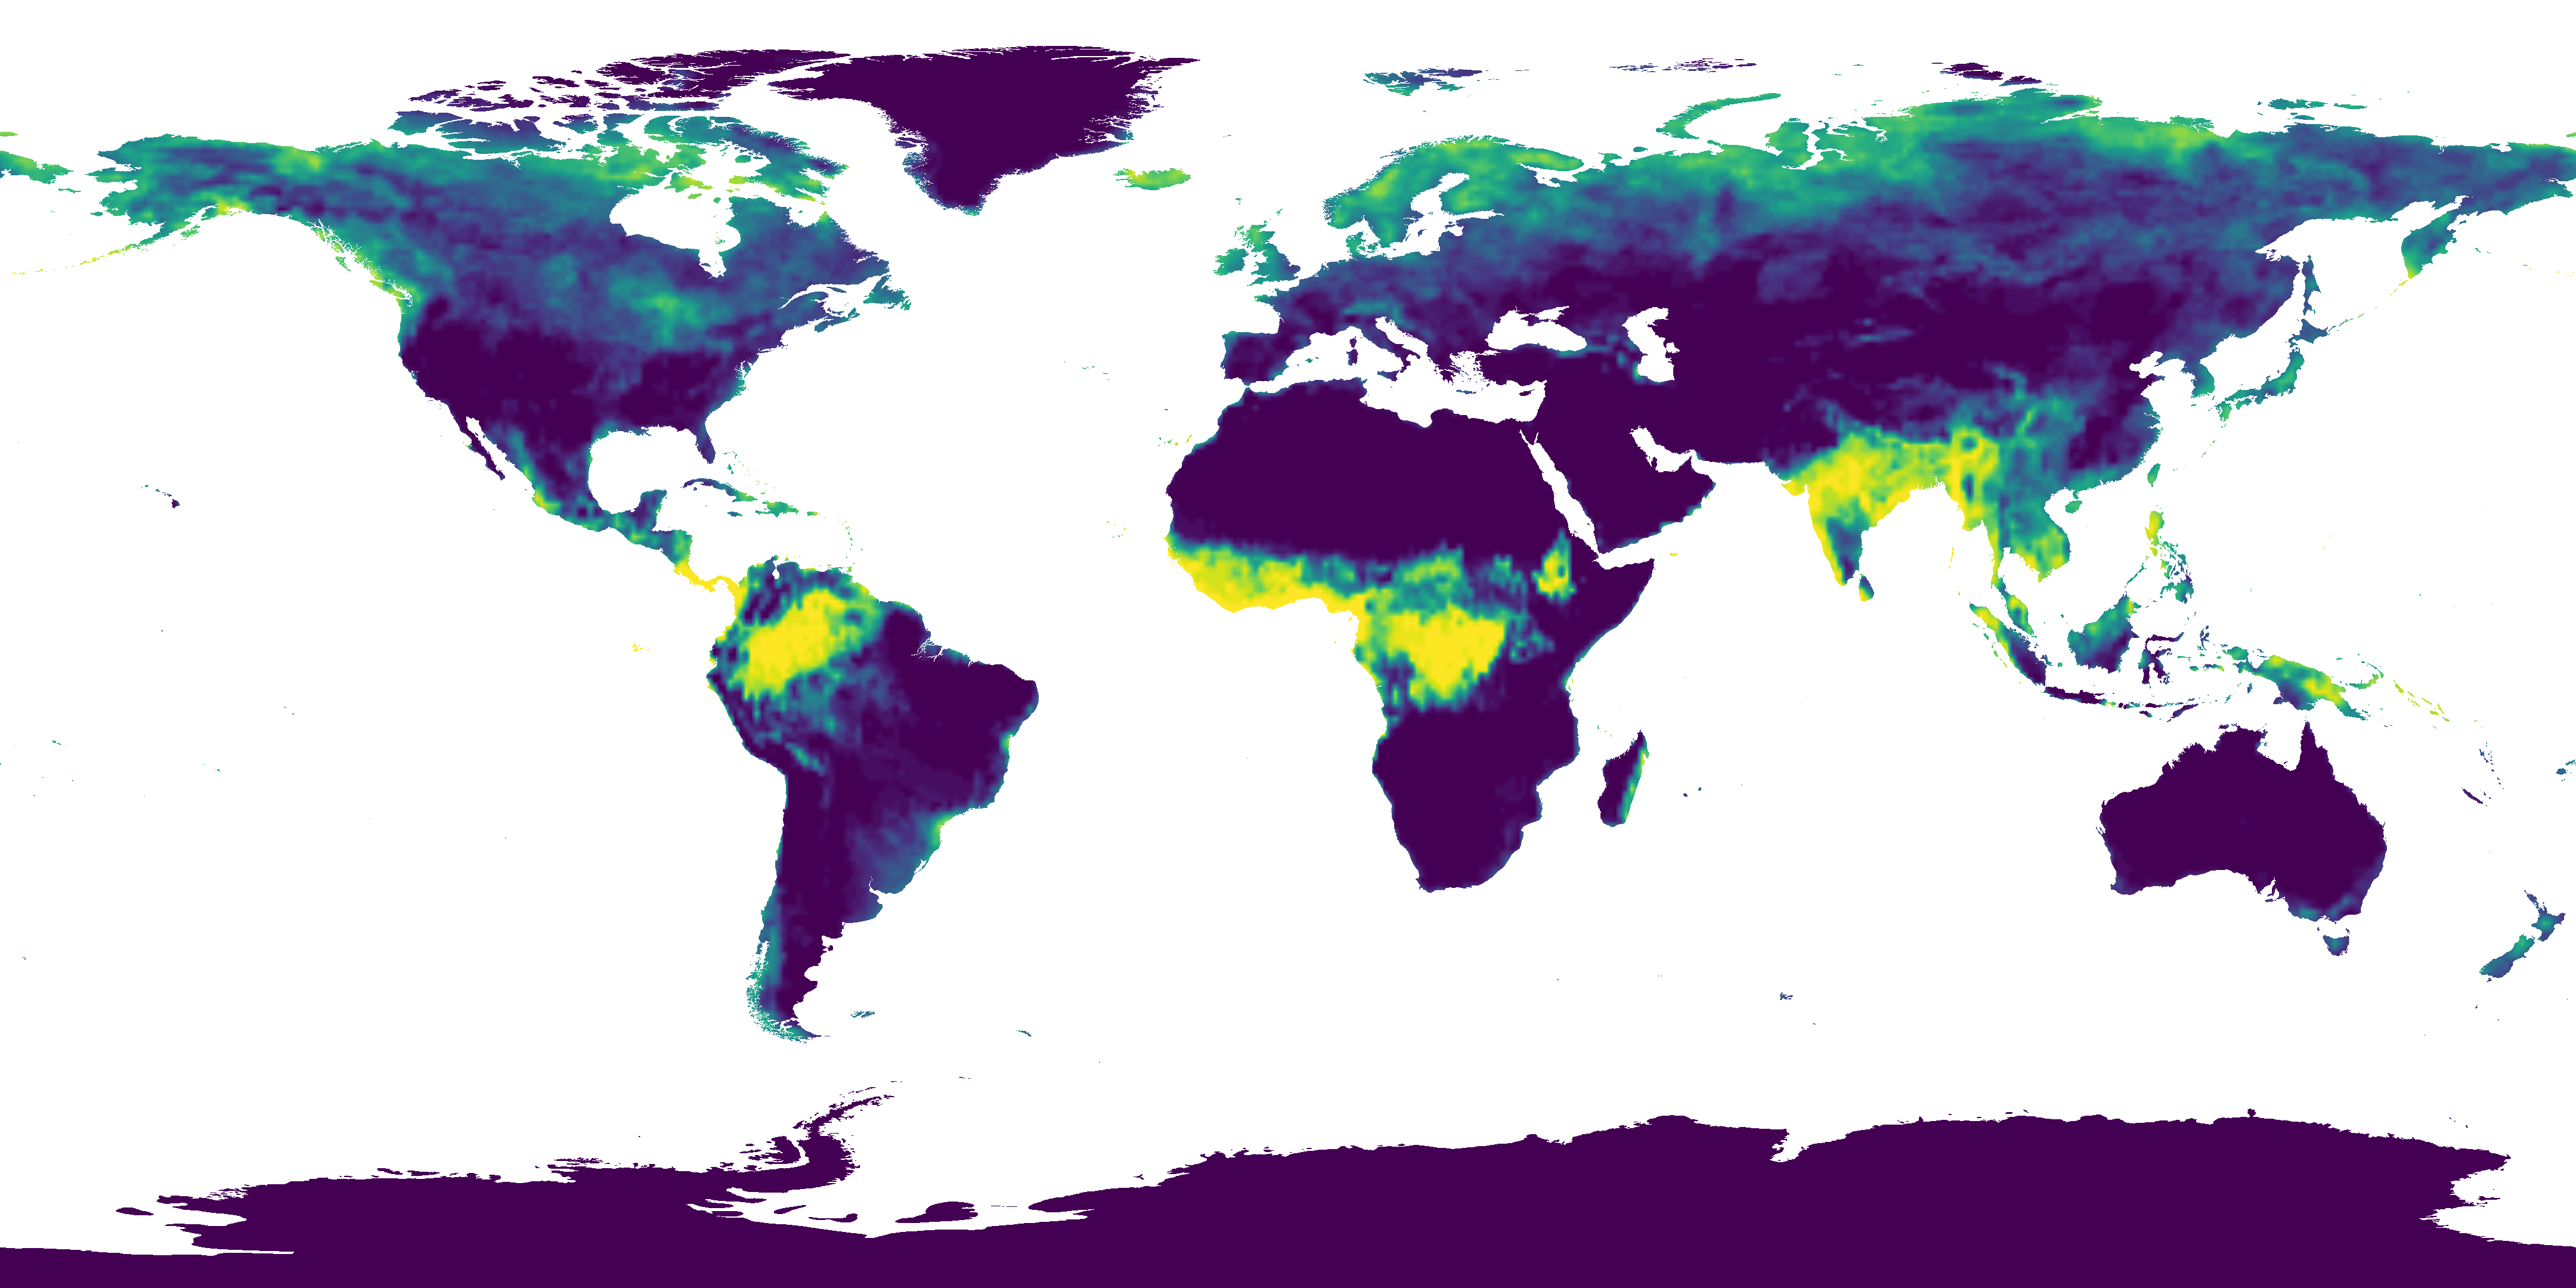
\includegraphics[width=.28\textwidth,height=2cm]{wet_monthly_2019_09_cropped_rescaled_4213da1e_897b_4887_8f78_6025b3977e3e.png}}\\
\subfloat[FOW October]{\label{sfig:d}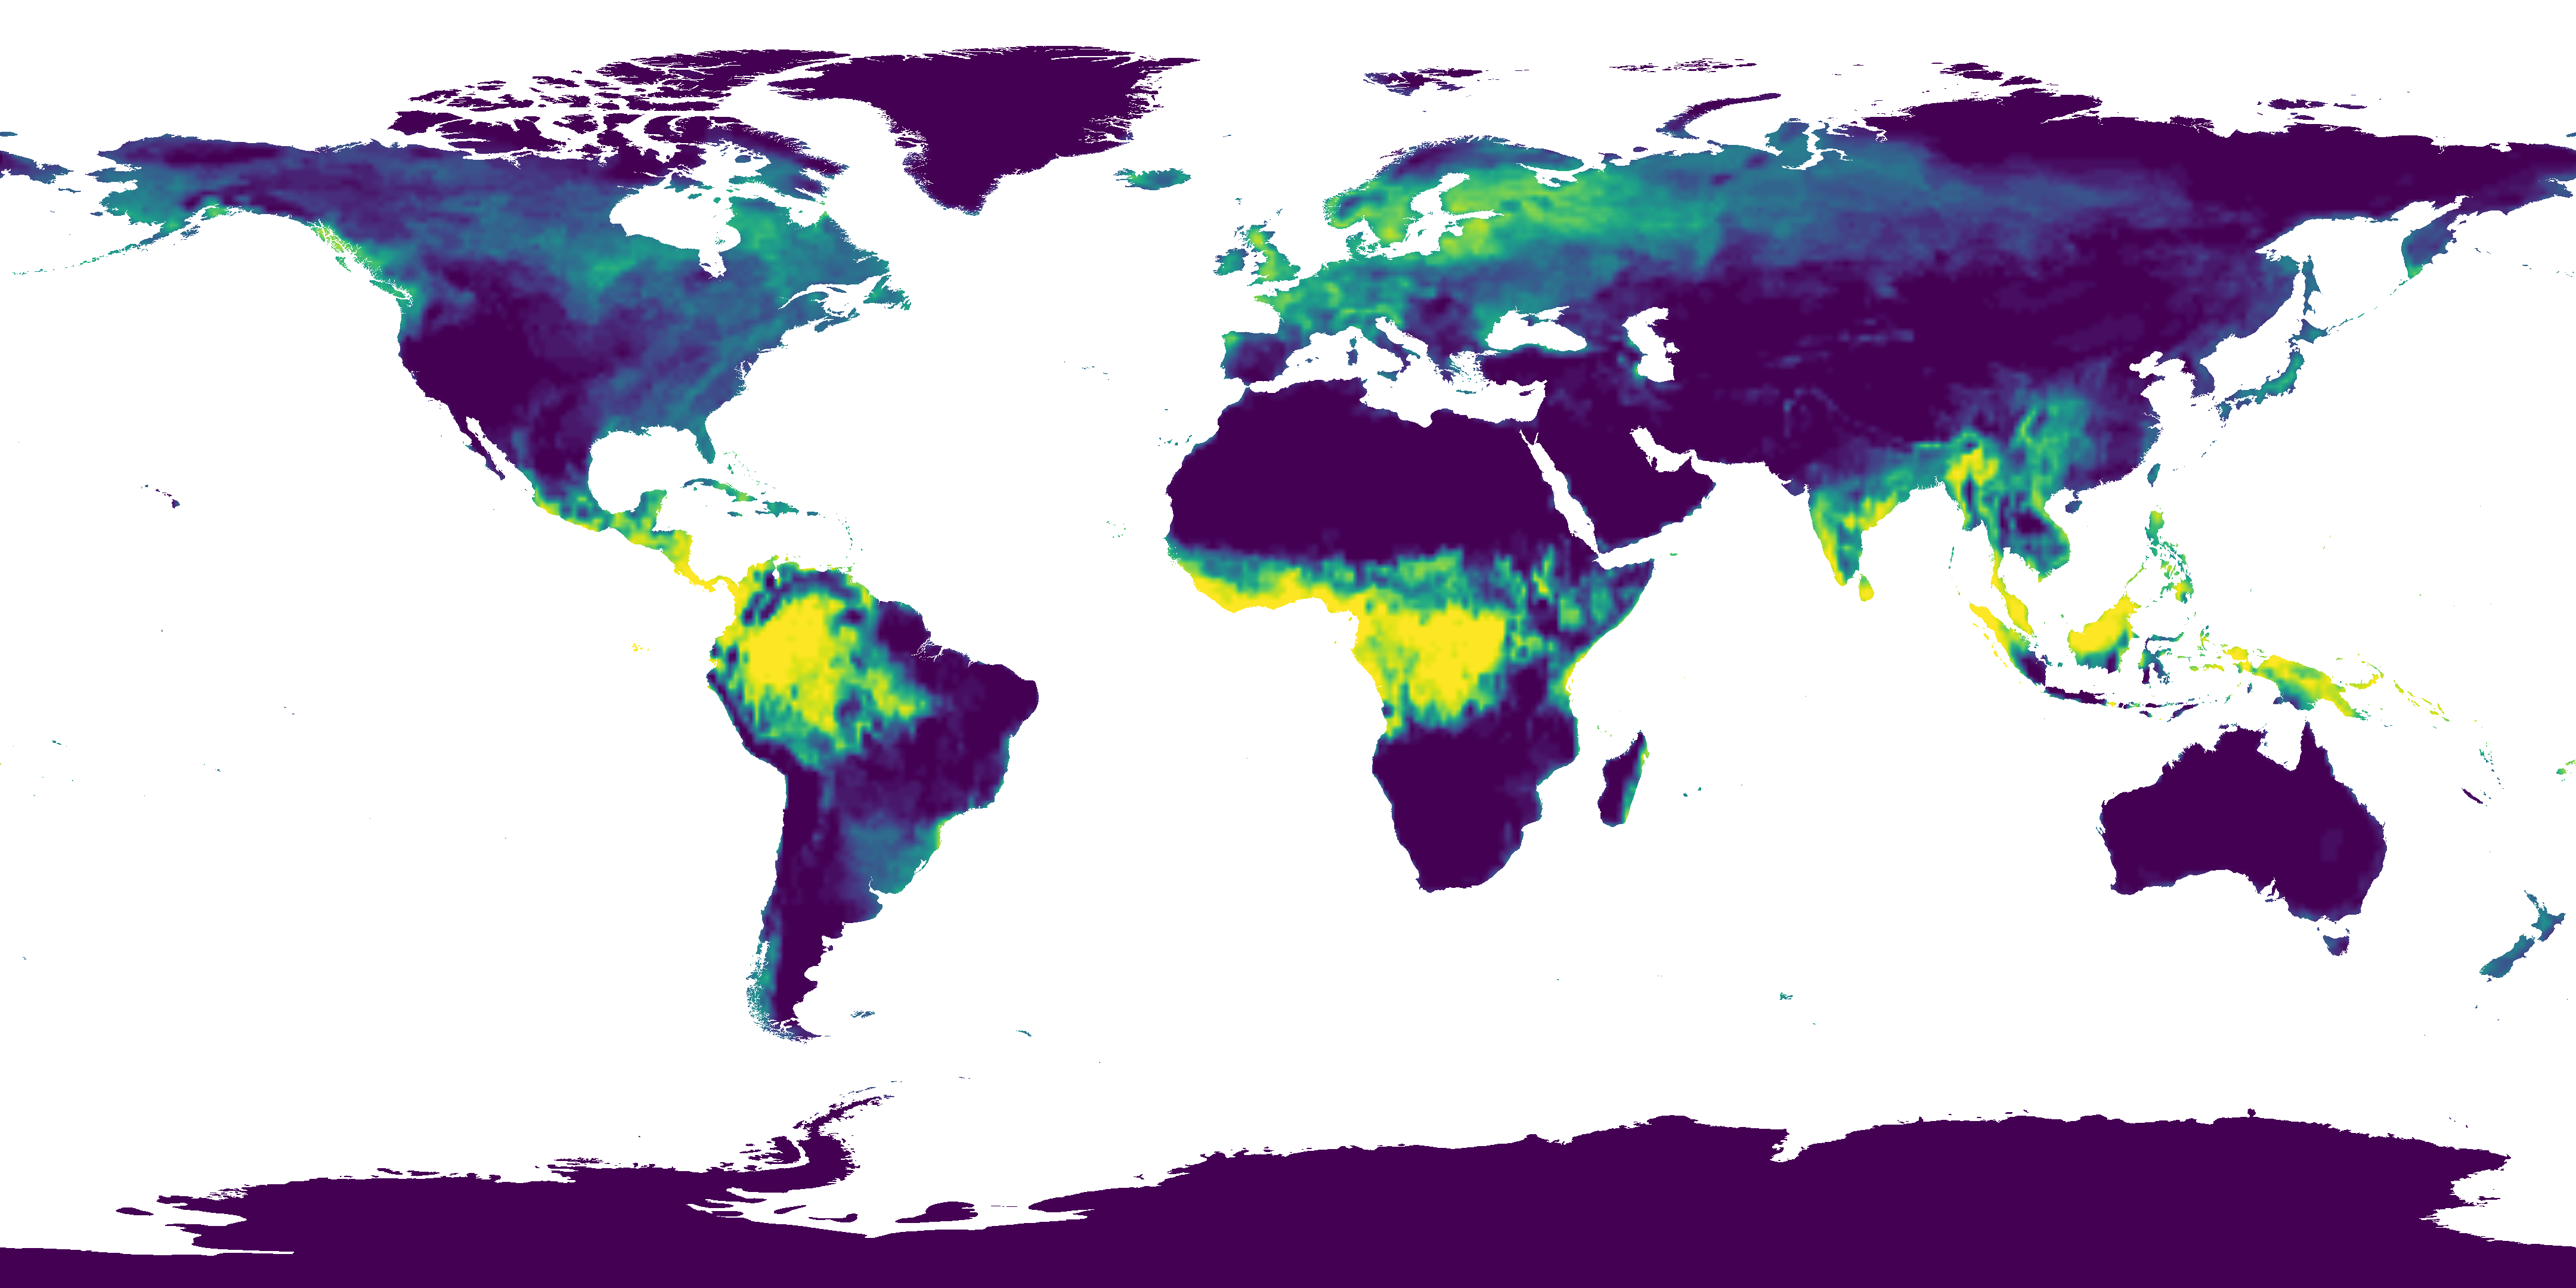
\includegraphics[width=.28\textwidth,height=2cm]{wet_monthly_2019_10_cropped_rescaled_c24ca636_b35e_46be_824a_ebbbfdeced48.png}}\hfill
\subfloat[FOW November]{\label{sfig:e}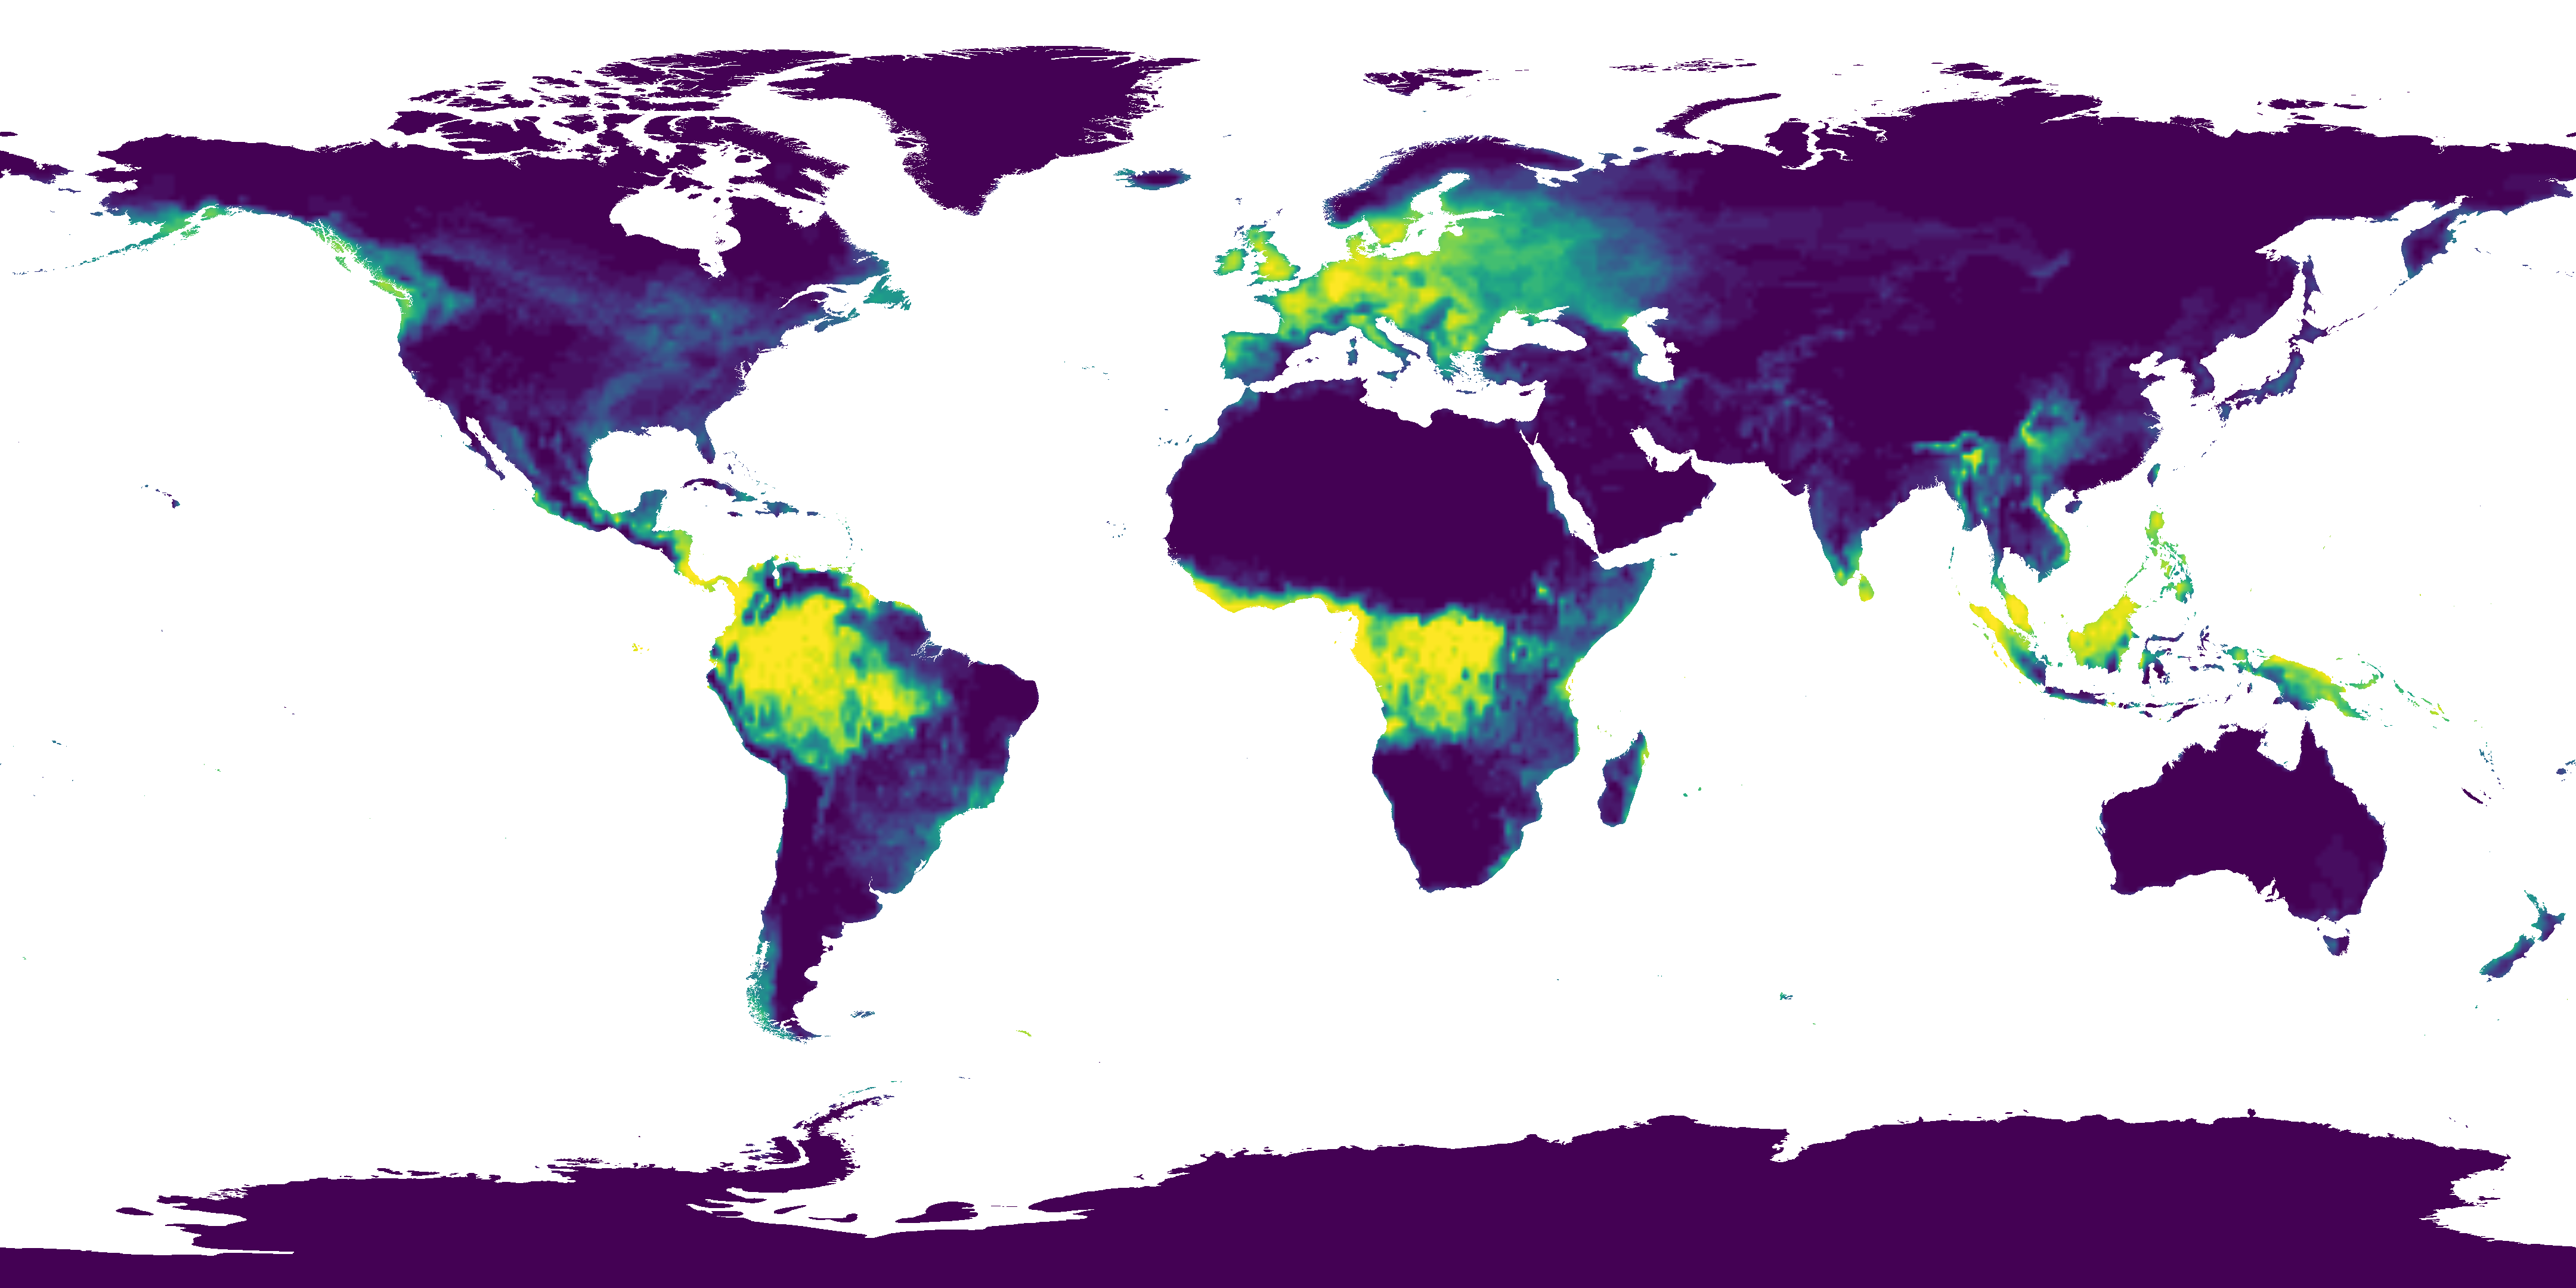
\includegraphics[width=.28\textwidth,height=2cm]{wet_monthly_2019_11_cropped_rescaled_bc379318_0e4f_4d6c_af62_cefec32a086a.png}}\hfill
\subfloat[FOW December]{\label{sfig:f}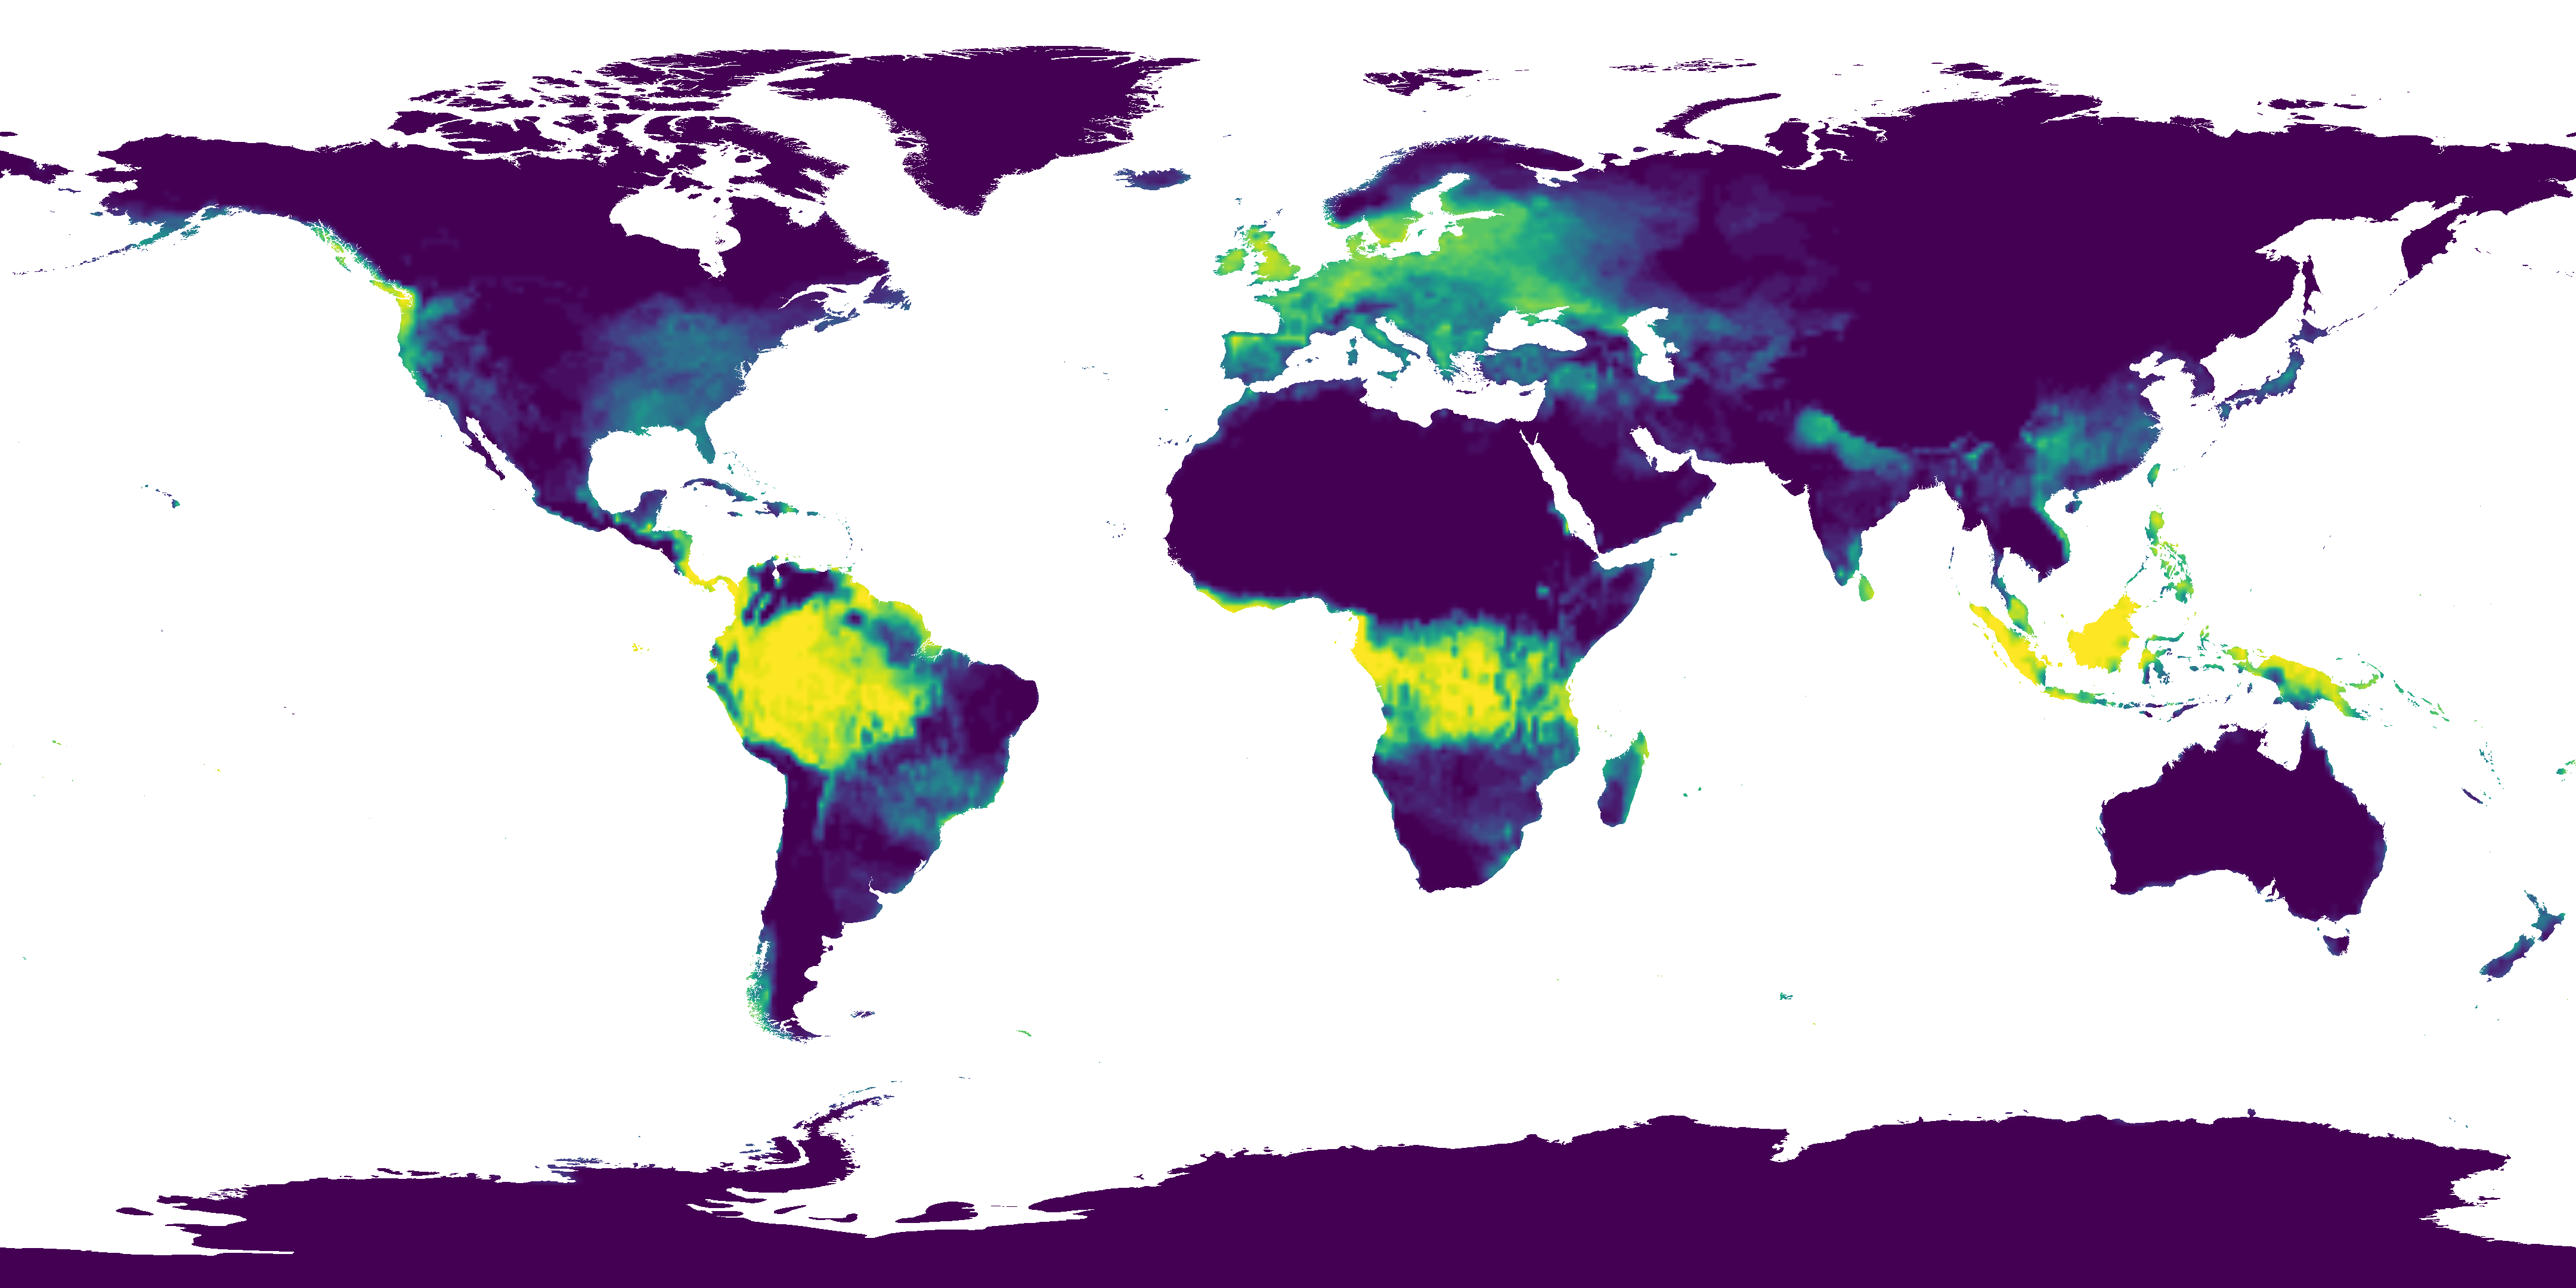
\includegraphics[width=.28\textwidth,height=2cm]{wet_monthly_2019_12_cropped_rescaled_69d54507_adfa_4afa_949e_c629f0f8cd3c.png}}\\
\caption{Frequency of wetness rasters for each month of the year}
\label{fig:FOW}
\end{figure}

\subsection{Hierarchical Clustering on Principle Components}
This analysis was conducted on a month by month basis using monthly averaged raster maps of Temperature, Precipitation, UV radiation, Salt aerosol concentration, Time of Wetness (TOW) and Frequency of Wetness (FOW) for each respective month. The output consists of twelve different clustering of ETS to compare how location similarities in ETS fluctuate throughout the year. These clusters can be seen in \ref{fig:jan_jun_ffp} and \ref{fig:jul_dec_ffp}. 

Prior to determining the clusters PCA is conducted on the raw data set for each month, this reduces the multivariate data set to a bivariate data set to allow better visualisation. Shown in Figure \ref{fig:scree} is the percentage of explained variance by each principle component for each month analysed. From this we can see that in all cases the first two principle components explain ~80\% of the total variation in the data set. This shows that the variability of the data set is well reflected in the first two principle components and that they will be suitable to use for classification in the next step.  

Figure \ref{fig:jan_jun_ffp_dend} and figure \ref{fig:jul_dec_ffp_dend} show the results of Hierarchical clustering carried out on the results of the PCA analysis of the data set. The parameters that determined the optimal number of clusters are detailed in section \ref{hcpc}. Figure \ref{fig:jan_jun_ffp} and Figure \ref{fig:jul_dec_ffp} show the results of PAM clustering carried out on the raw data. Both Hierarchical and PAM clustering assign ETS to the same clusters on a consistent basis. This give confidence in the robustness of the results. The clustering confirms some similarities in location that are intuitively obvious. For example Felling and Sunderland, Songjiang and Pudong, Florida 1 and Florida 2 are all clustered together in the same cluster for all 12 months. Intuitively from their close geographic proximity to each other it would be clear that these local climates are very similar. Although this is not a ground-breaking insight it does provide some confidence that the clustering is performing well and returning results that agree with fundamental understanding. 

\begin{figure}[H]
\centering
\subfloat[January Hierarchical Clustering]{\label{sfig:a}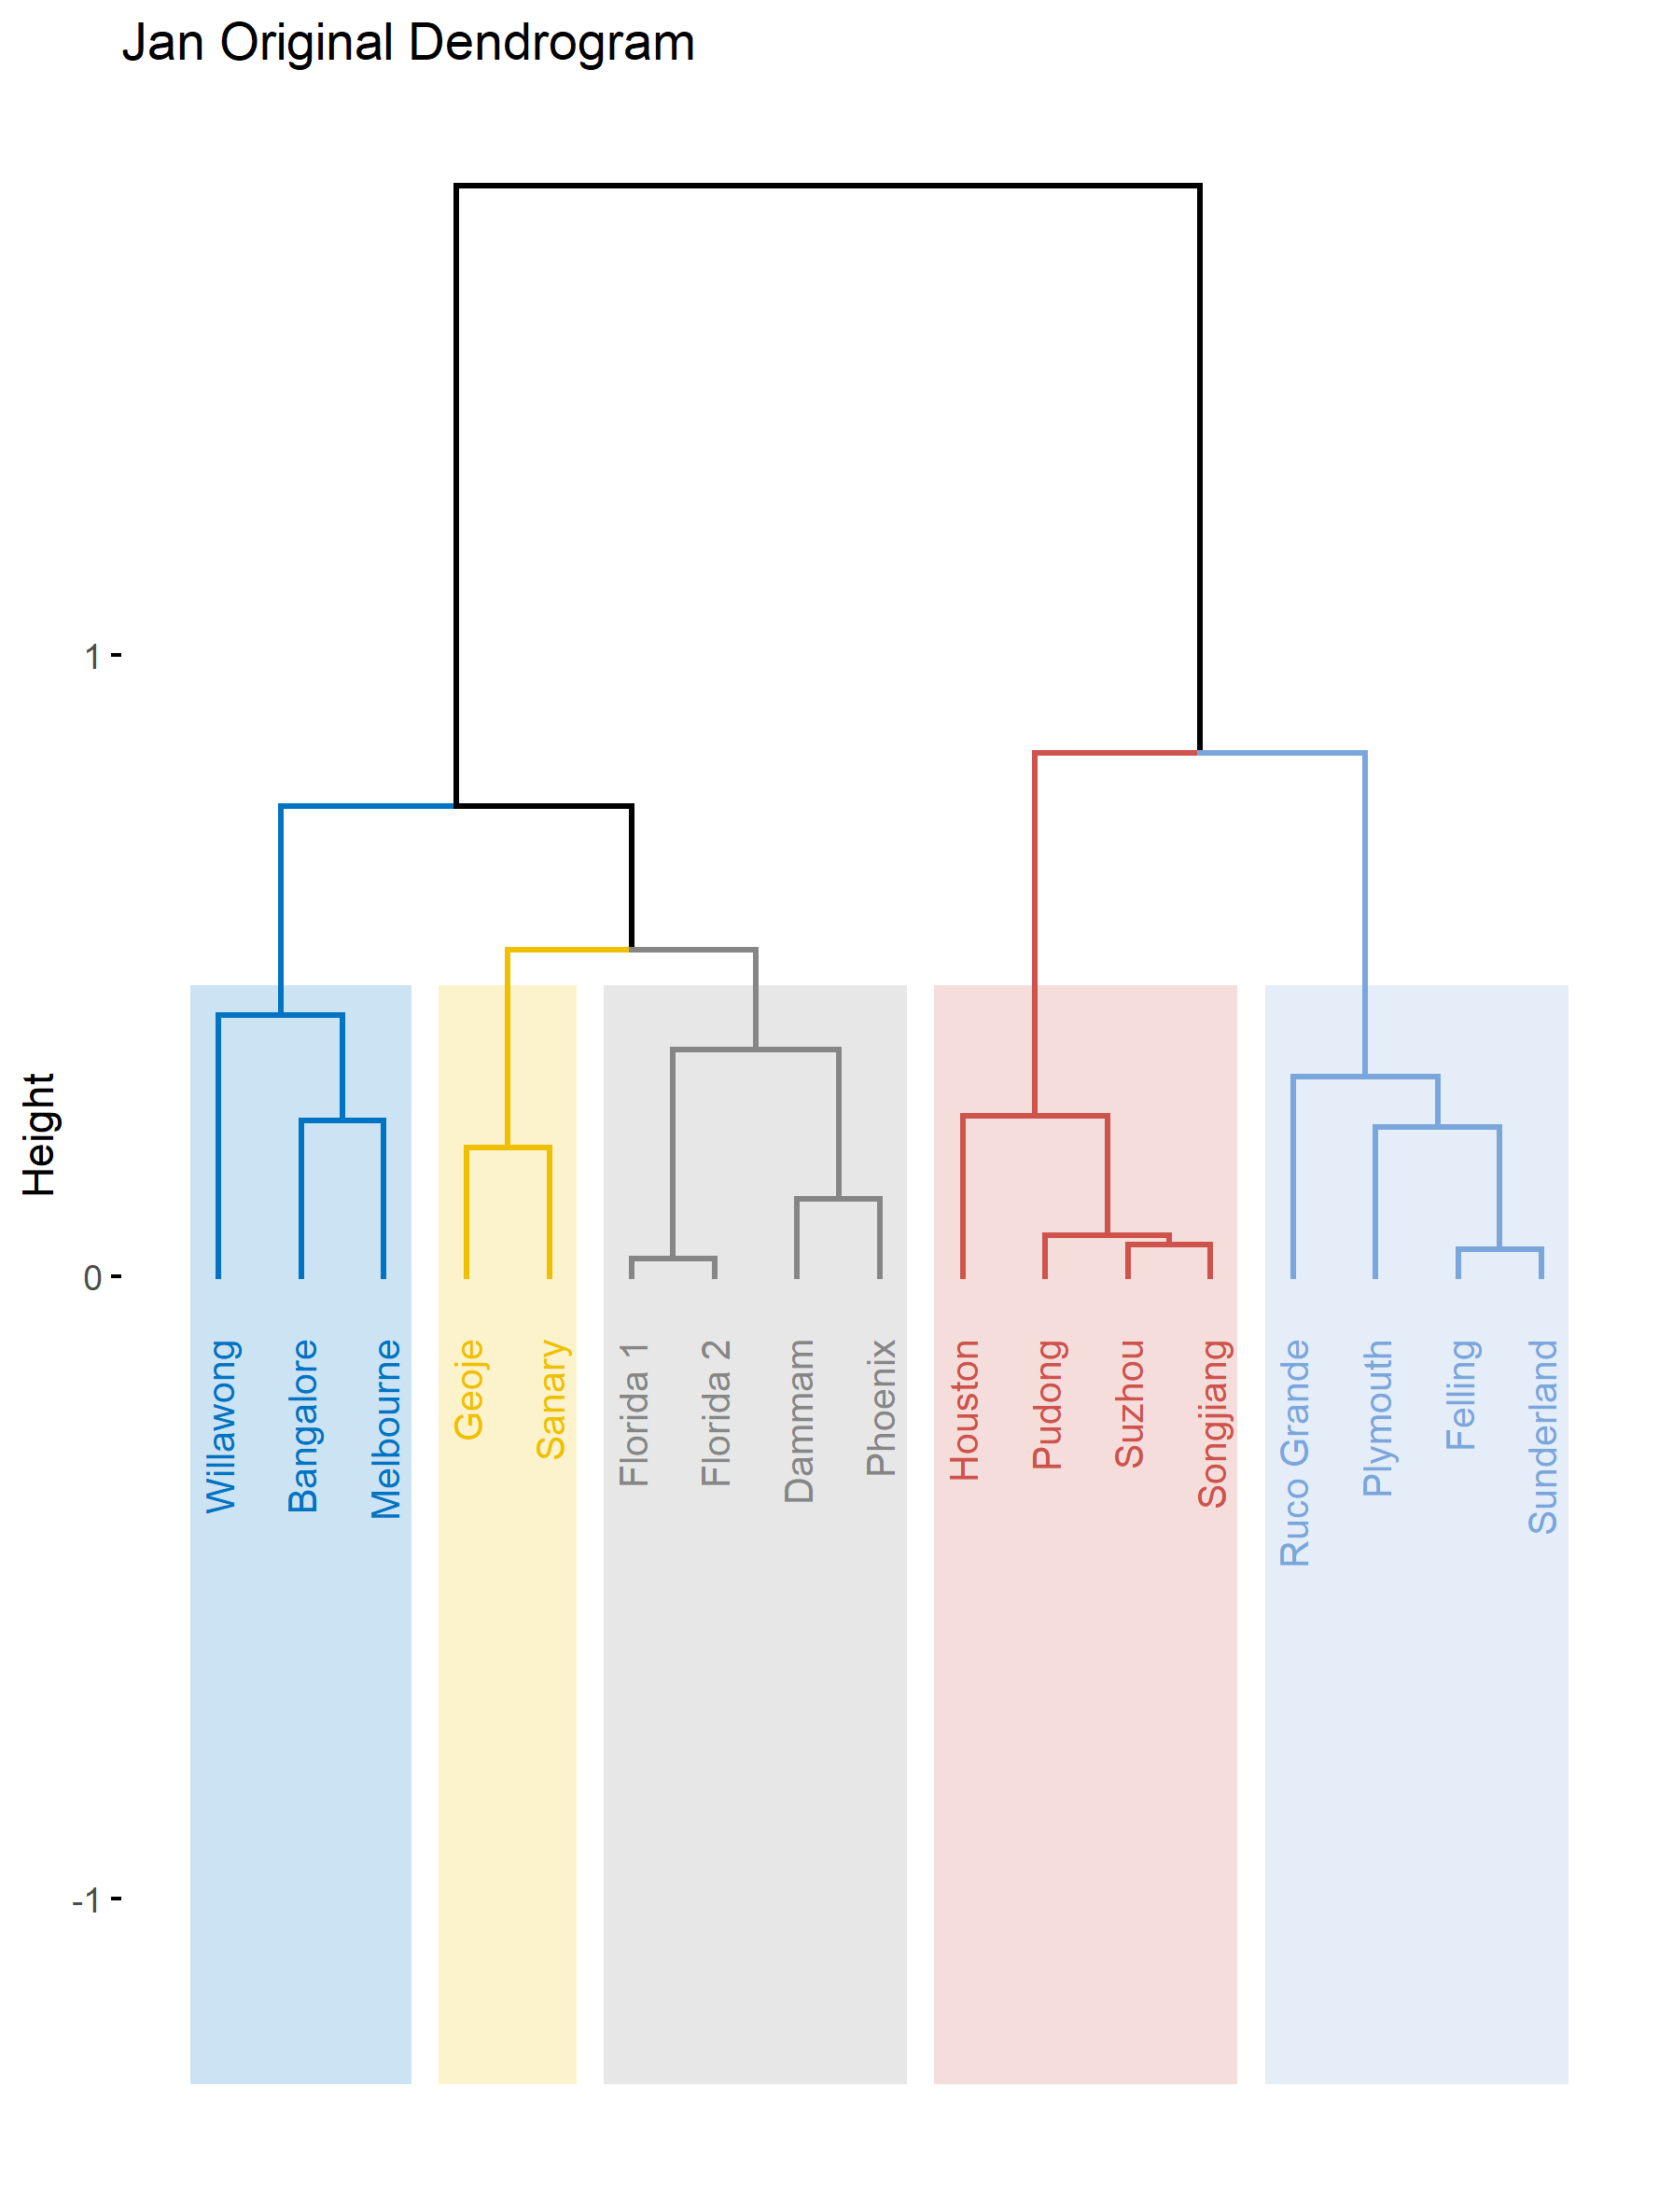
\includegraphics[width=.48\textwidth,height=6.5cm]{Jan_dend.png}}\hfill
\subfloat[February Hierarchical Clustering]{\label{sfig:b}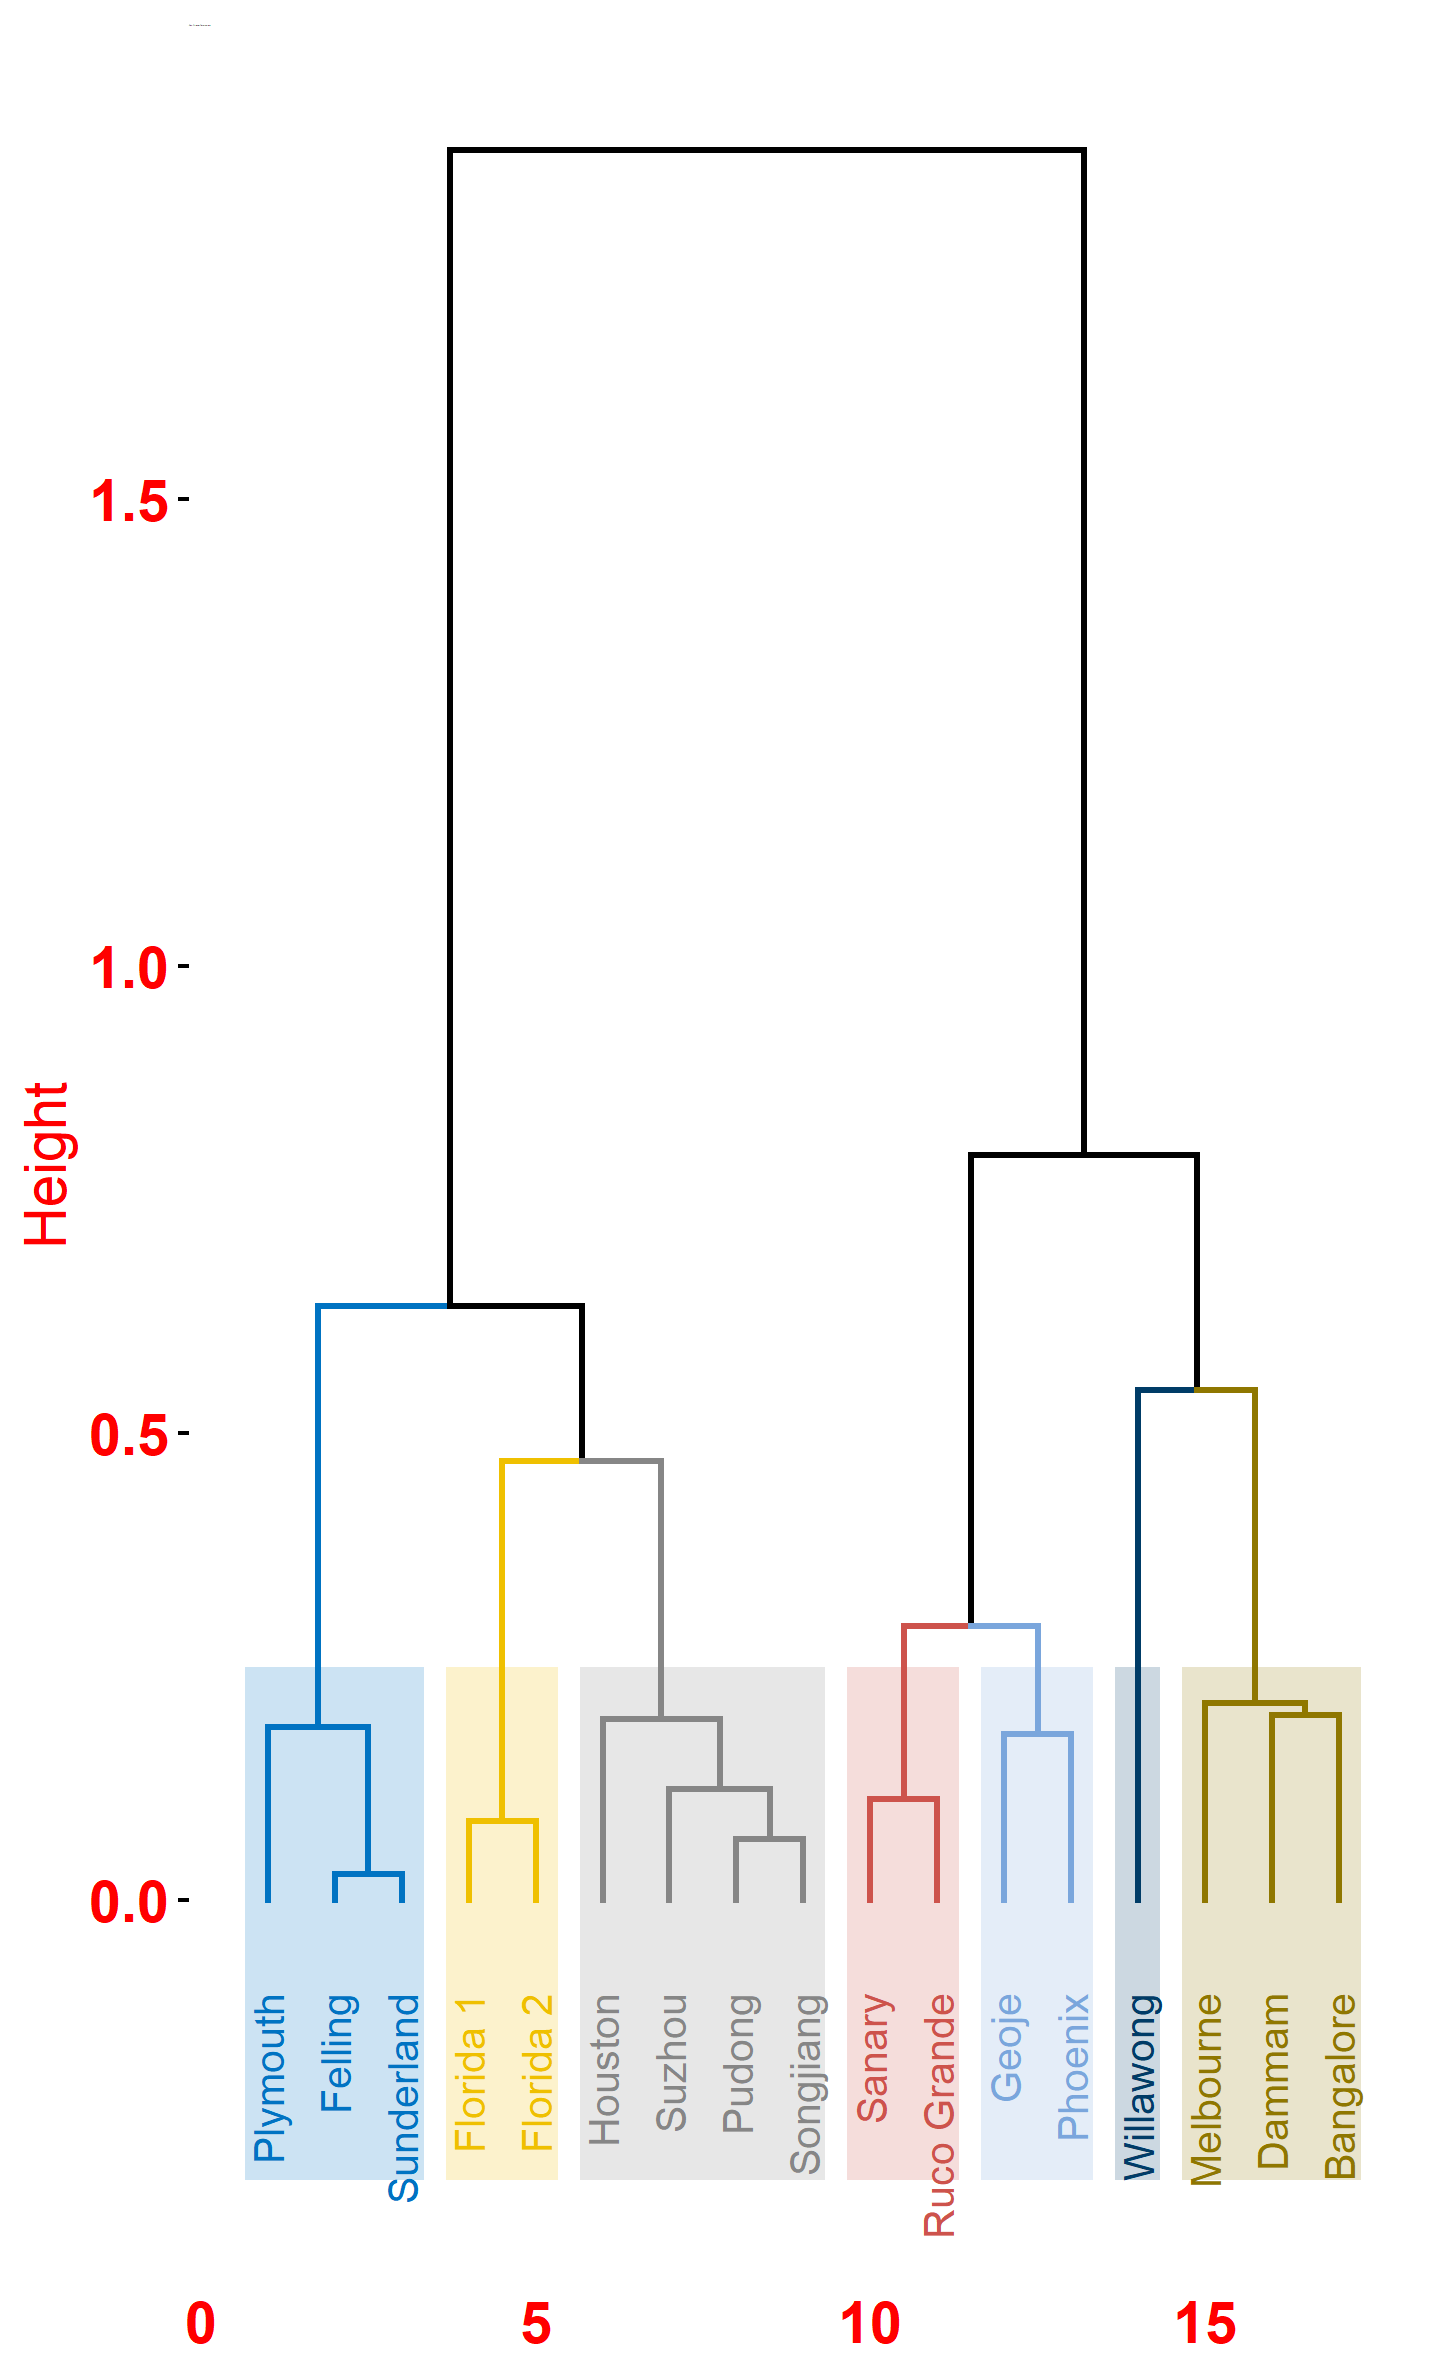
\includegraphics[width=.48\textwidth,height=6.5cm]{Feb_dend.png}}\\
\subfloat[March Hierarchical Clustering]{\label{sfig:c}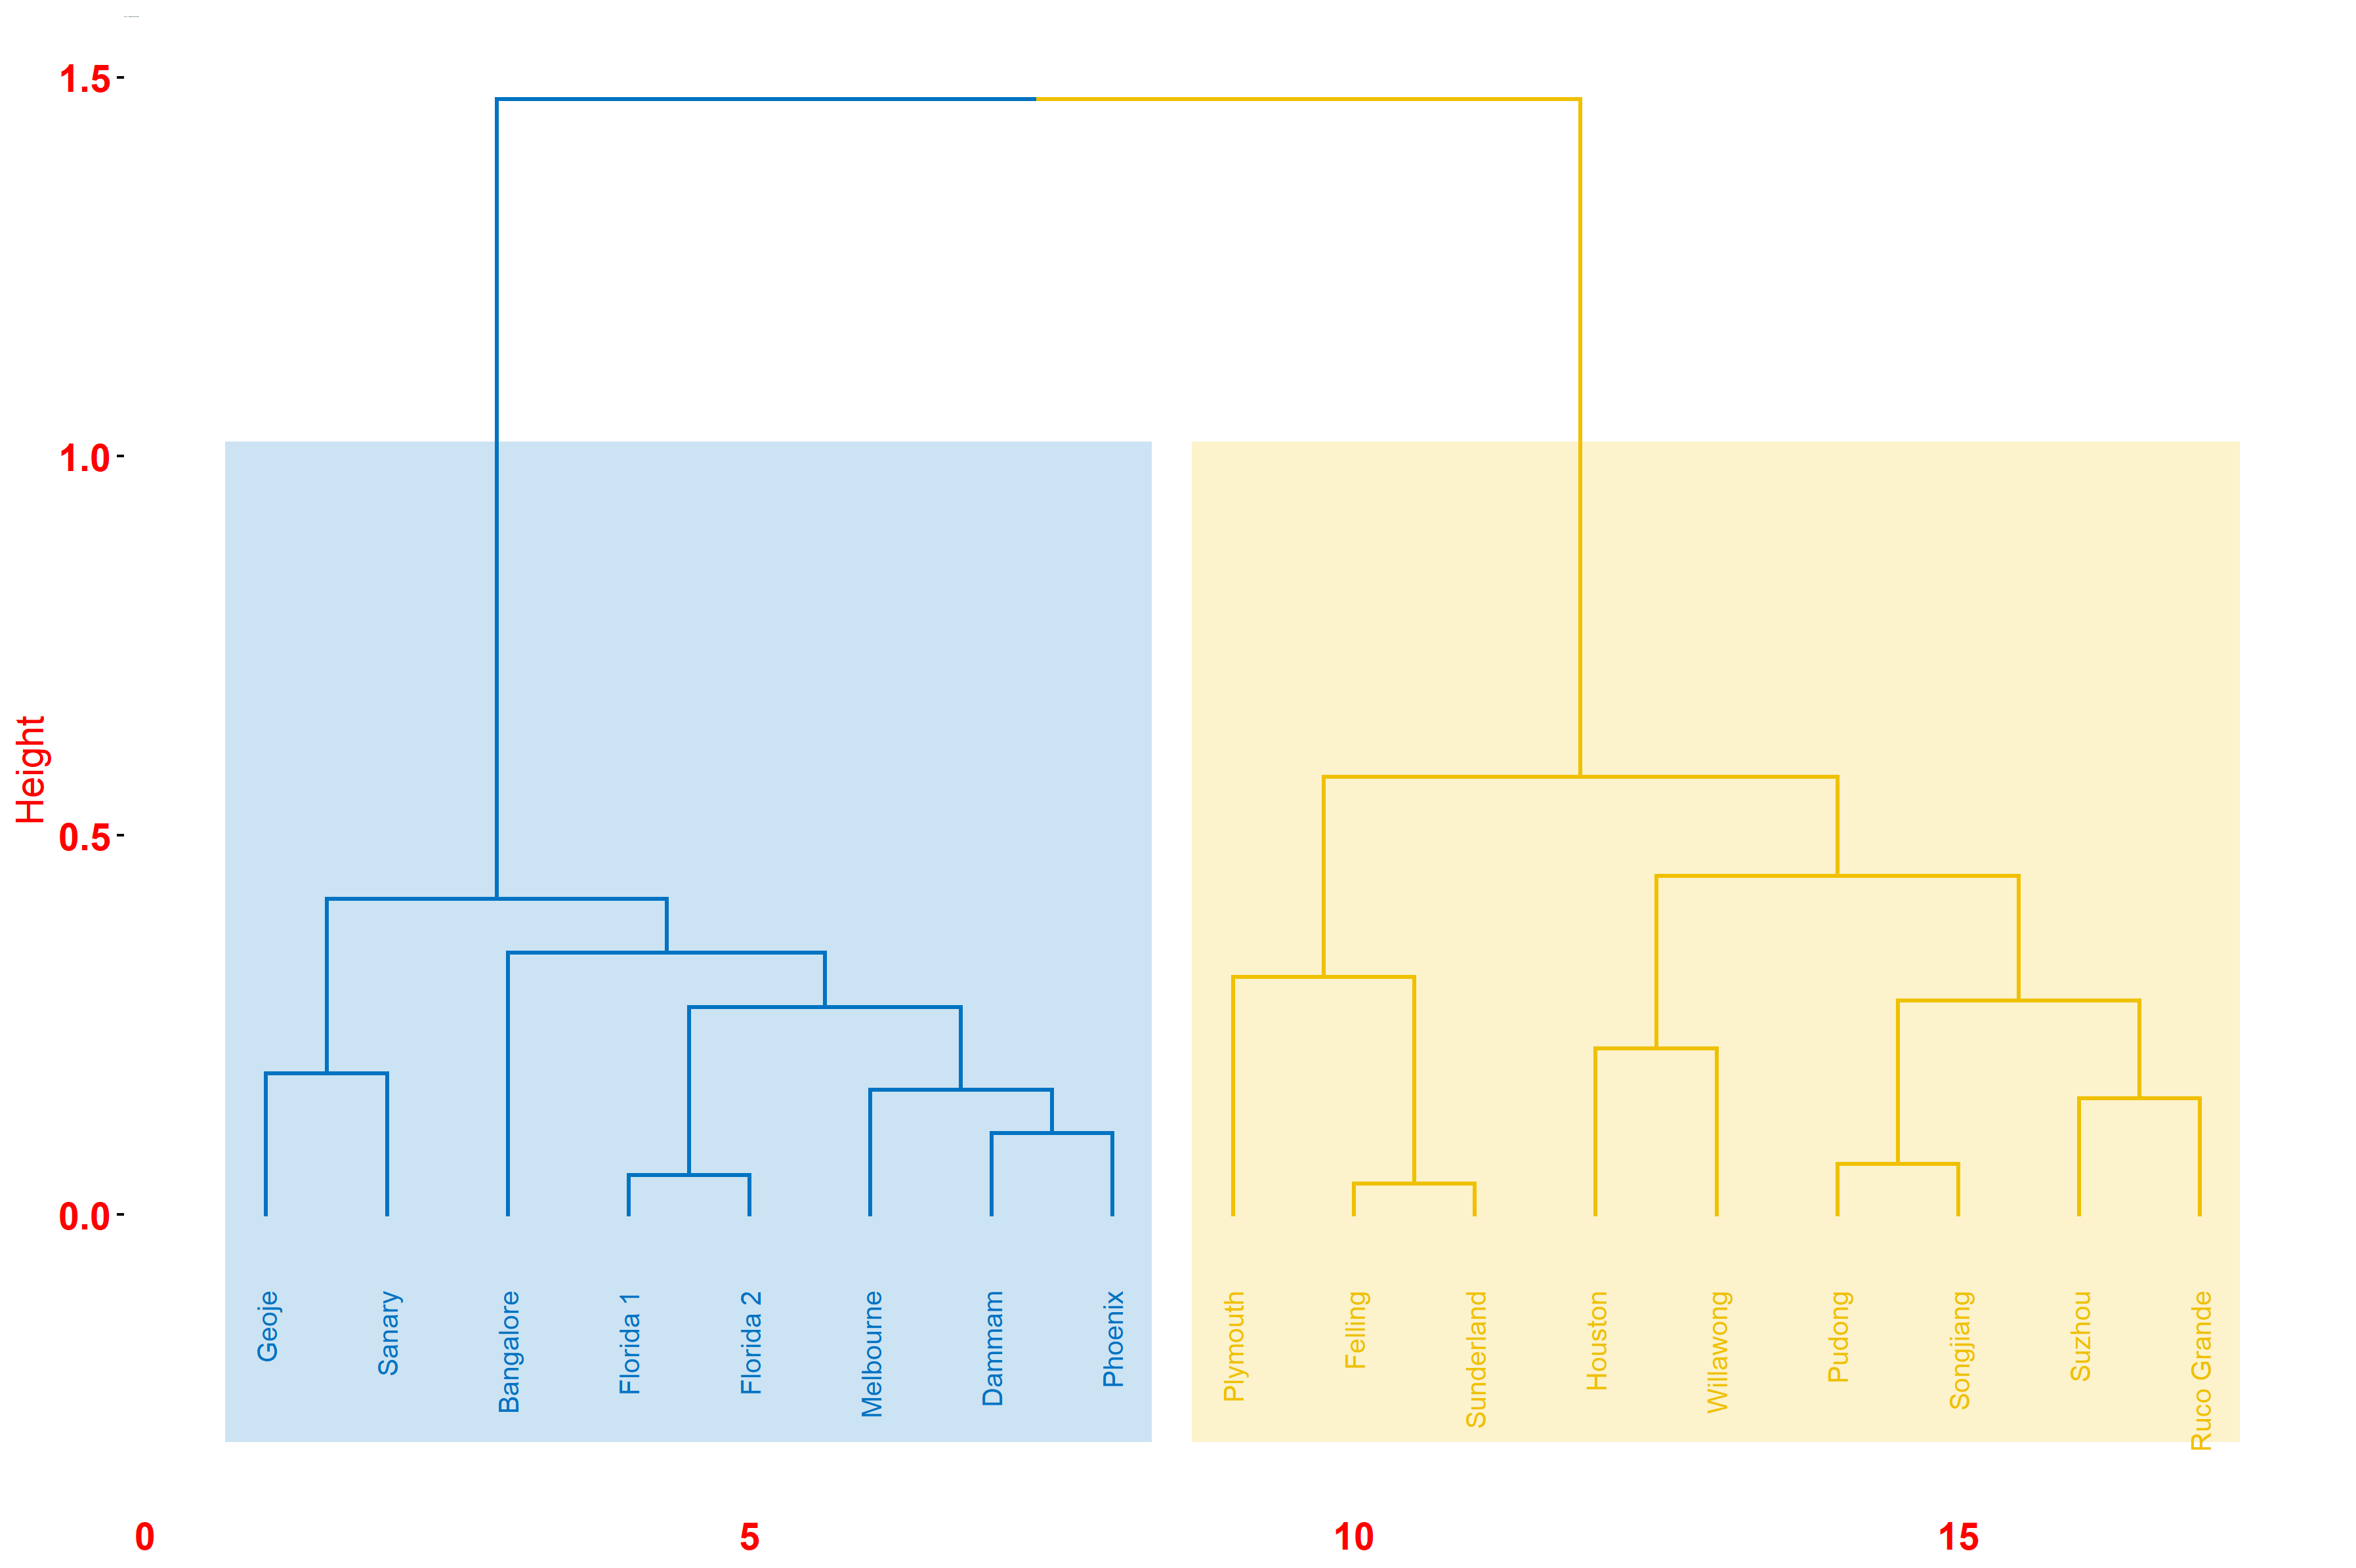
\includegraphics[width=.48\textwidth,height=6.5cm]{Mar_dend.png}}\hfill
\subfloat[April Hierarchical Clustering]{\label{sfig:d}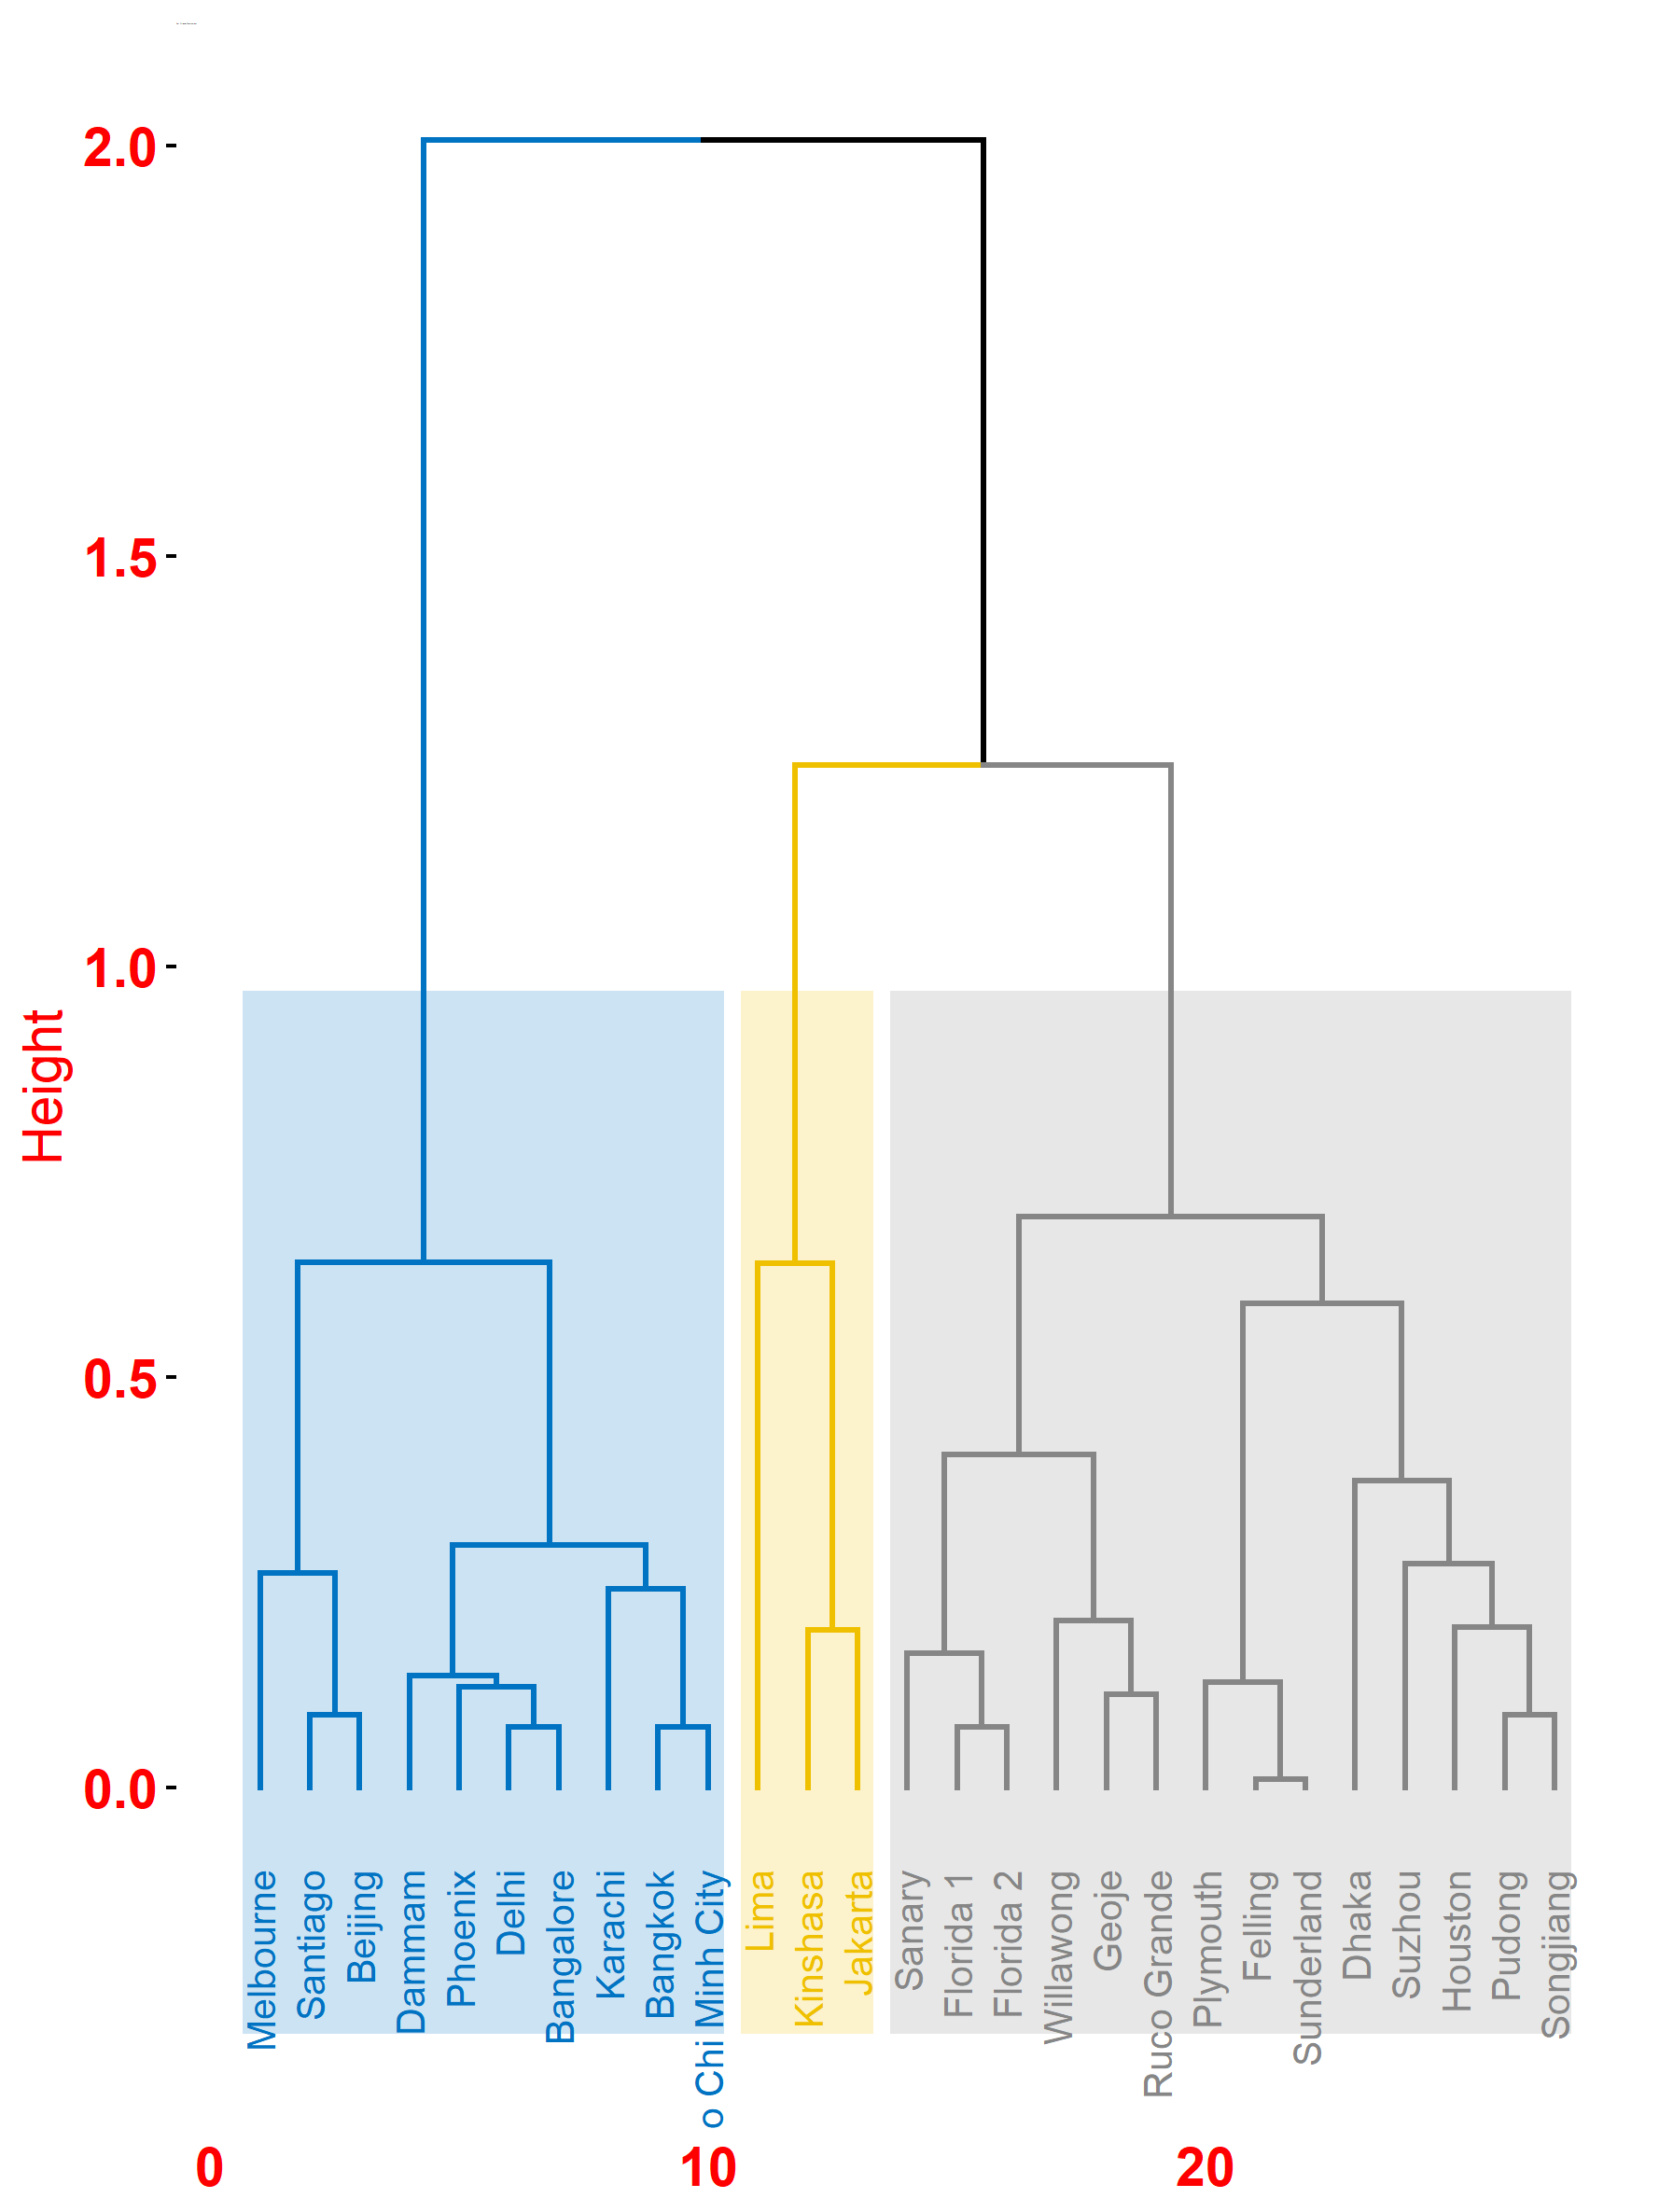
\includegraphics[width=.48\textwidth,height=6.5cm]{Apr_dend.png}}\\
\subfloat[May Hierarchical Clustering]{\label{sfig:e}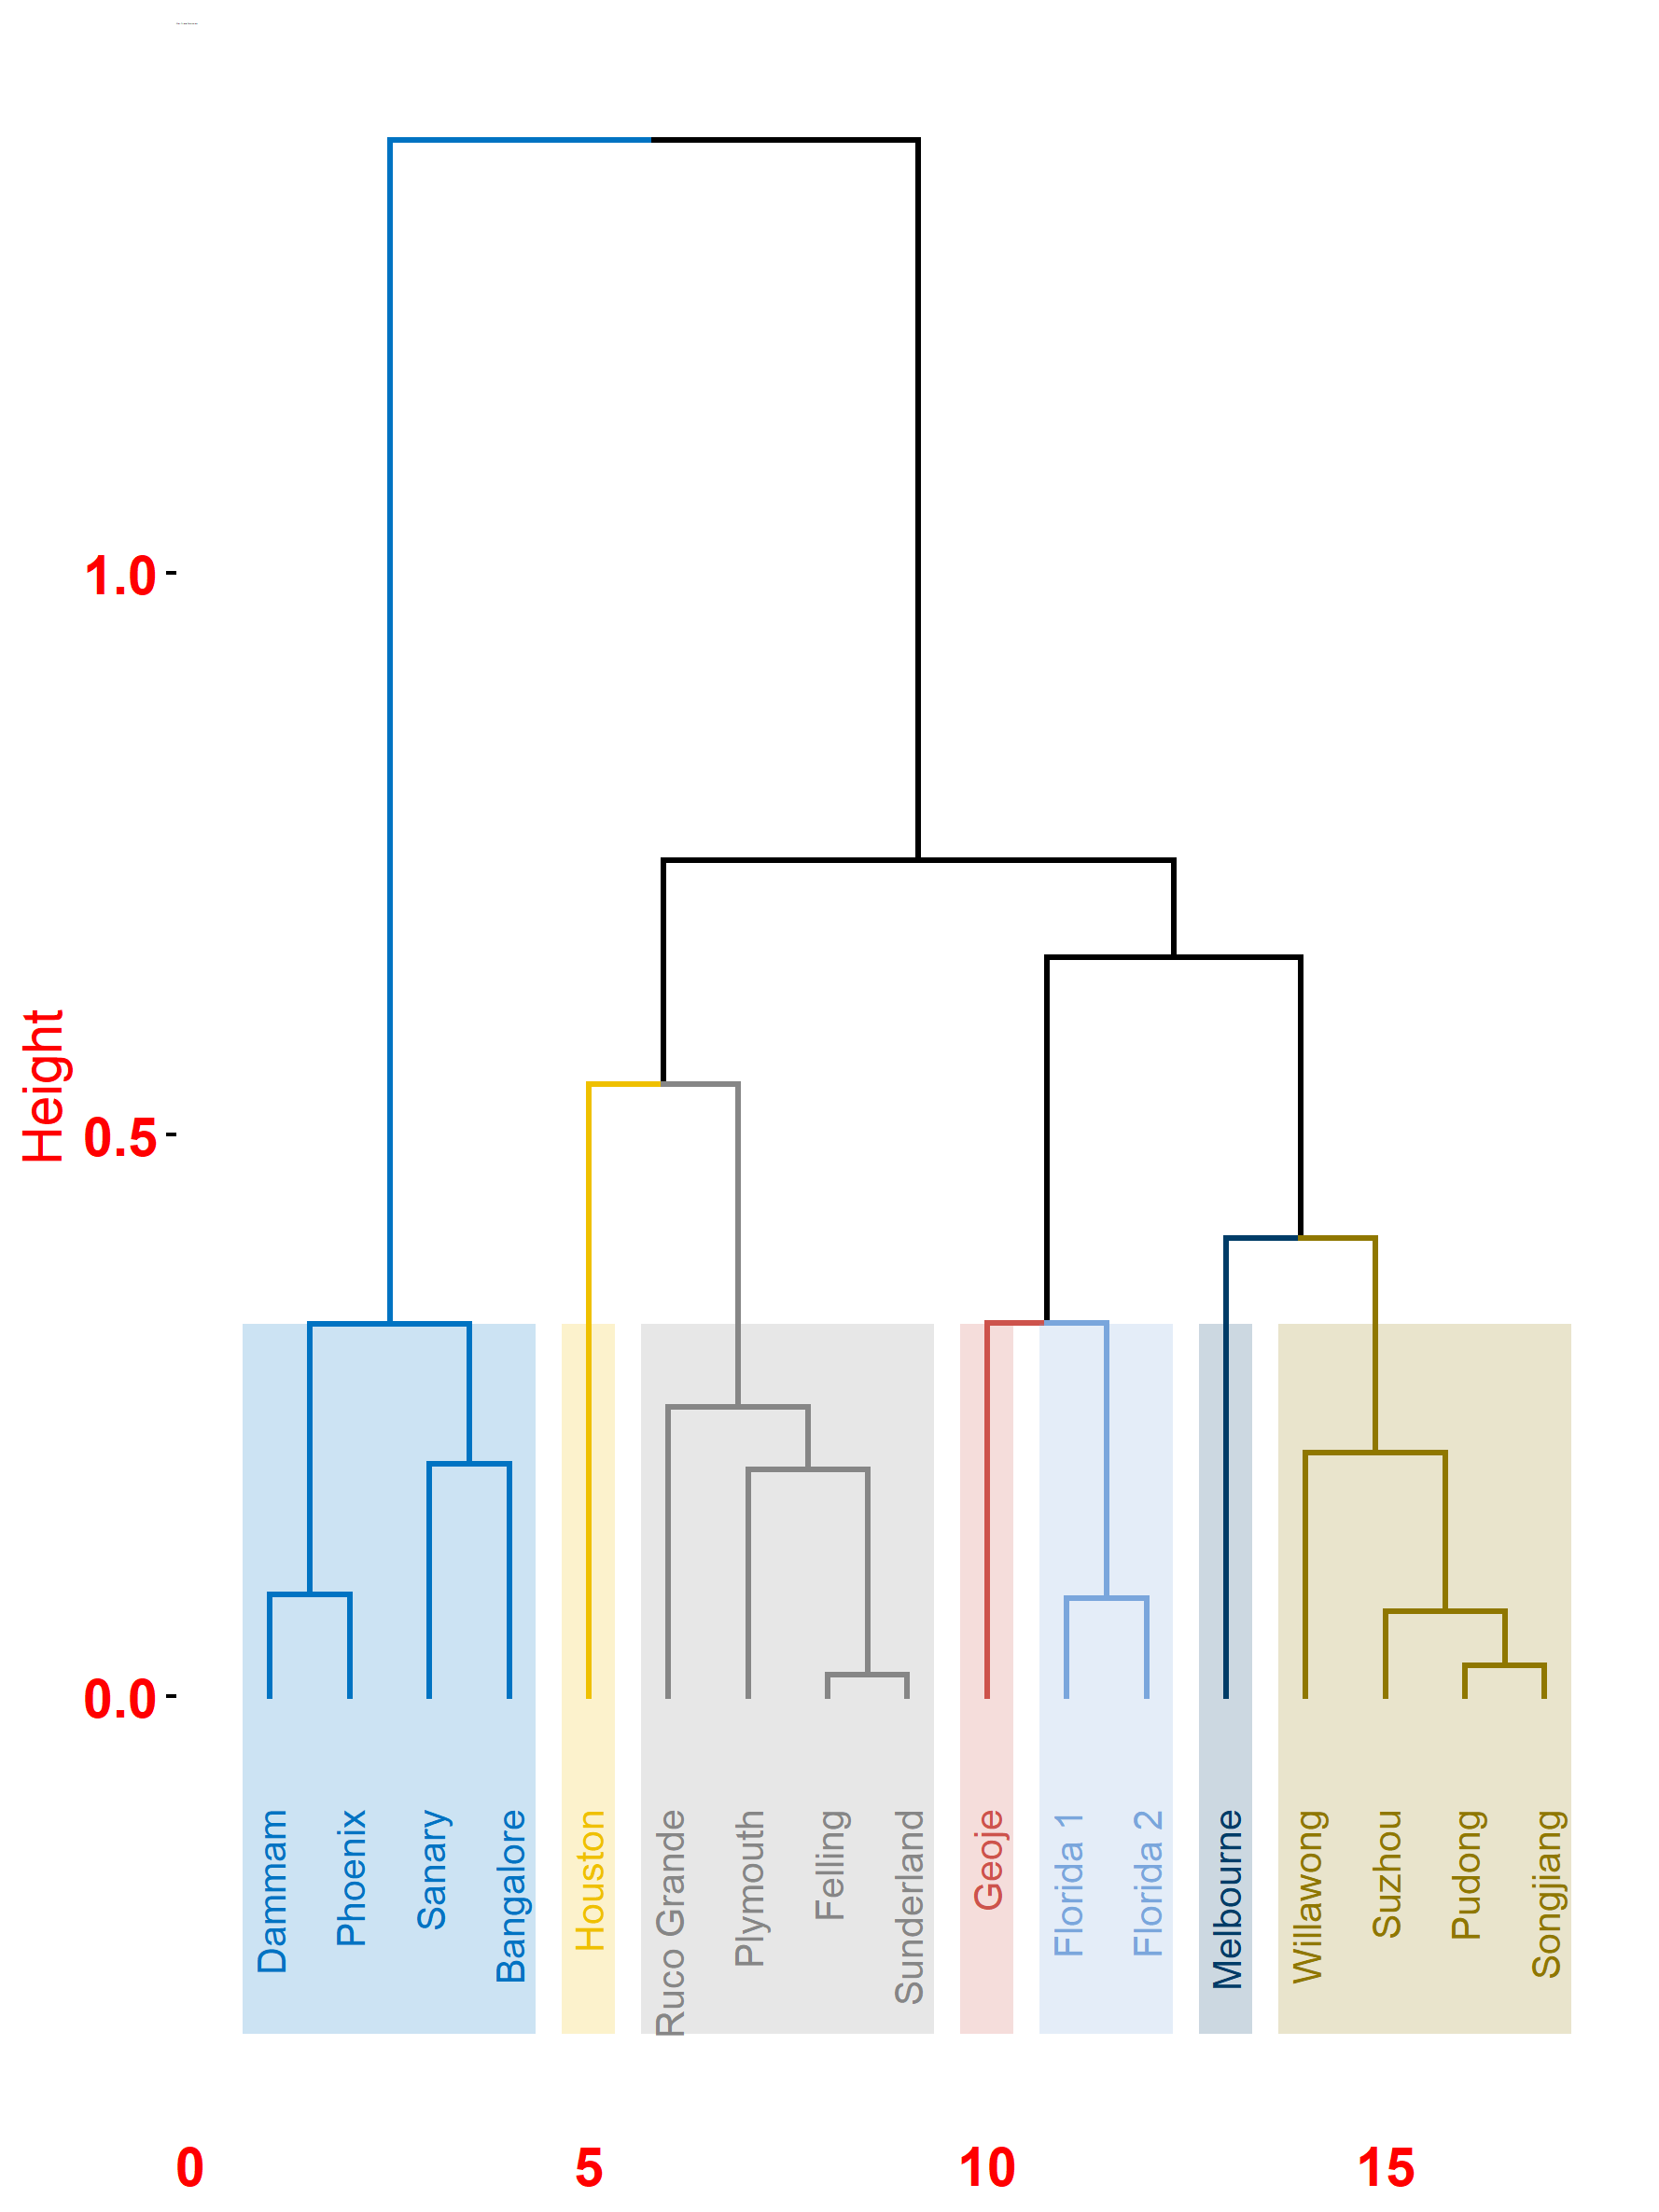
\includegraphics[width=.48\textwidth,height=6.5cm]{May_dend.png}}\hfill
\subfloat[June Hierarchical Clustering]{\label{sfig:f}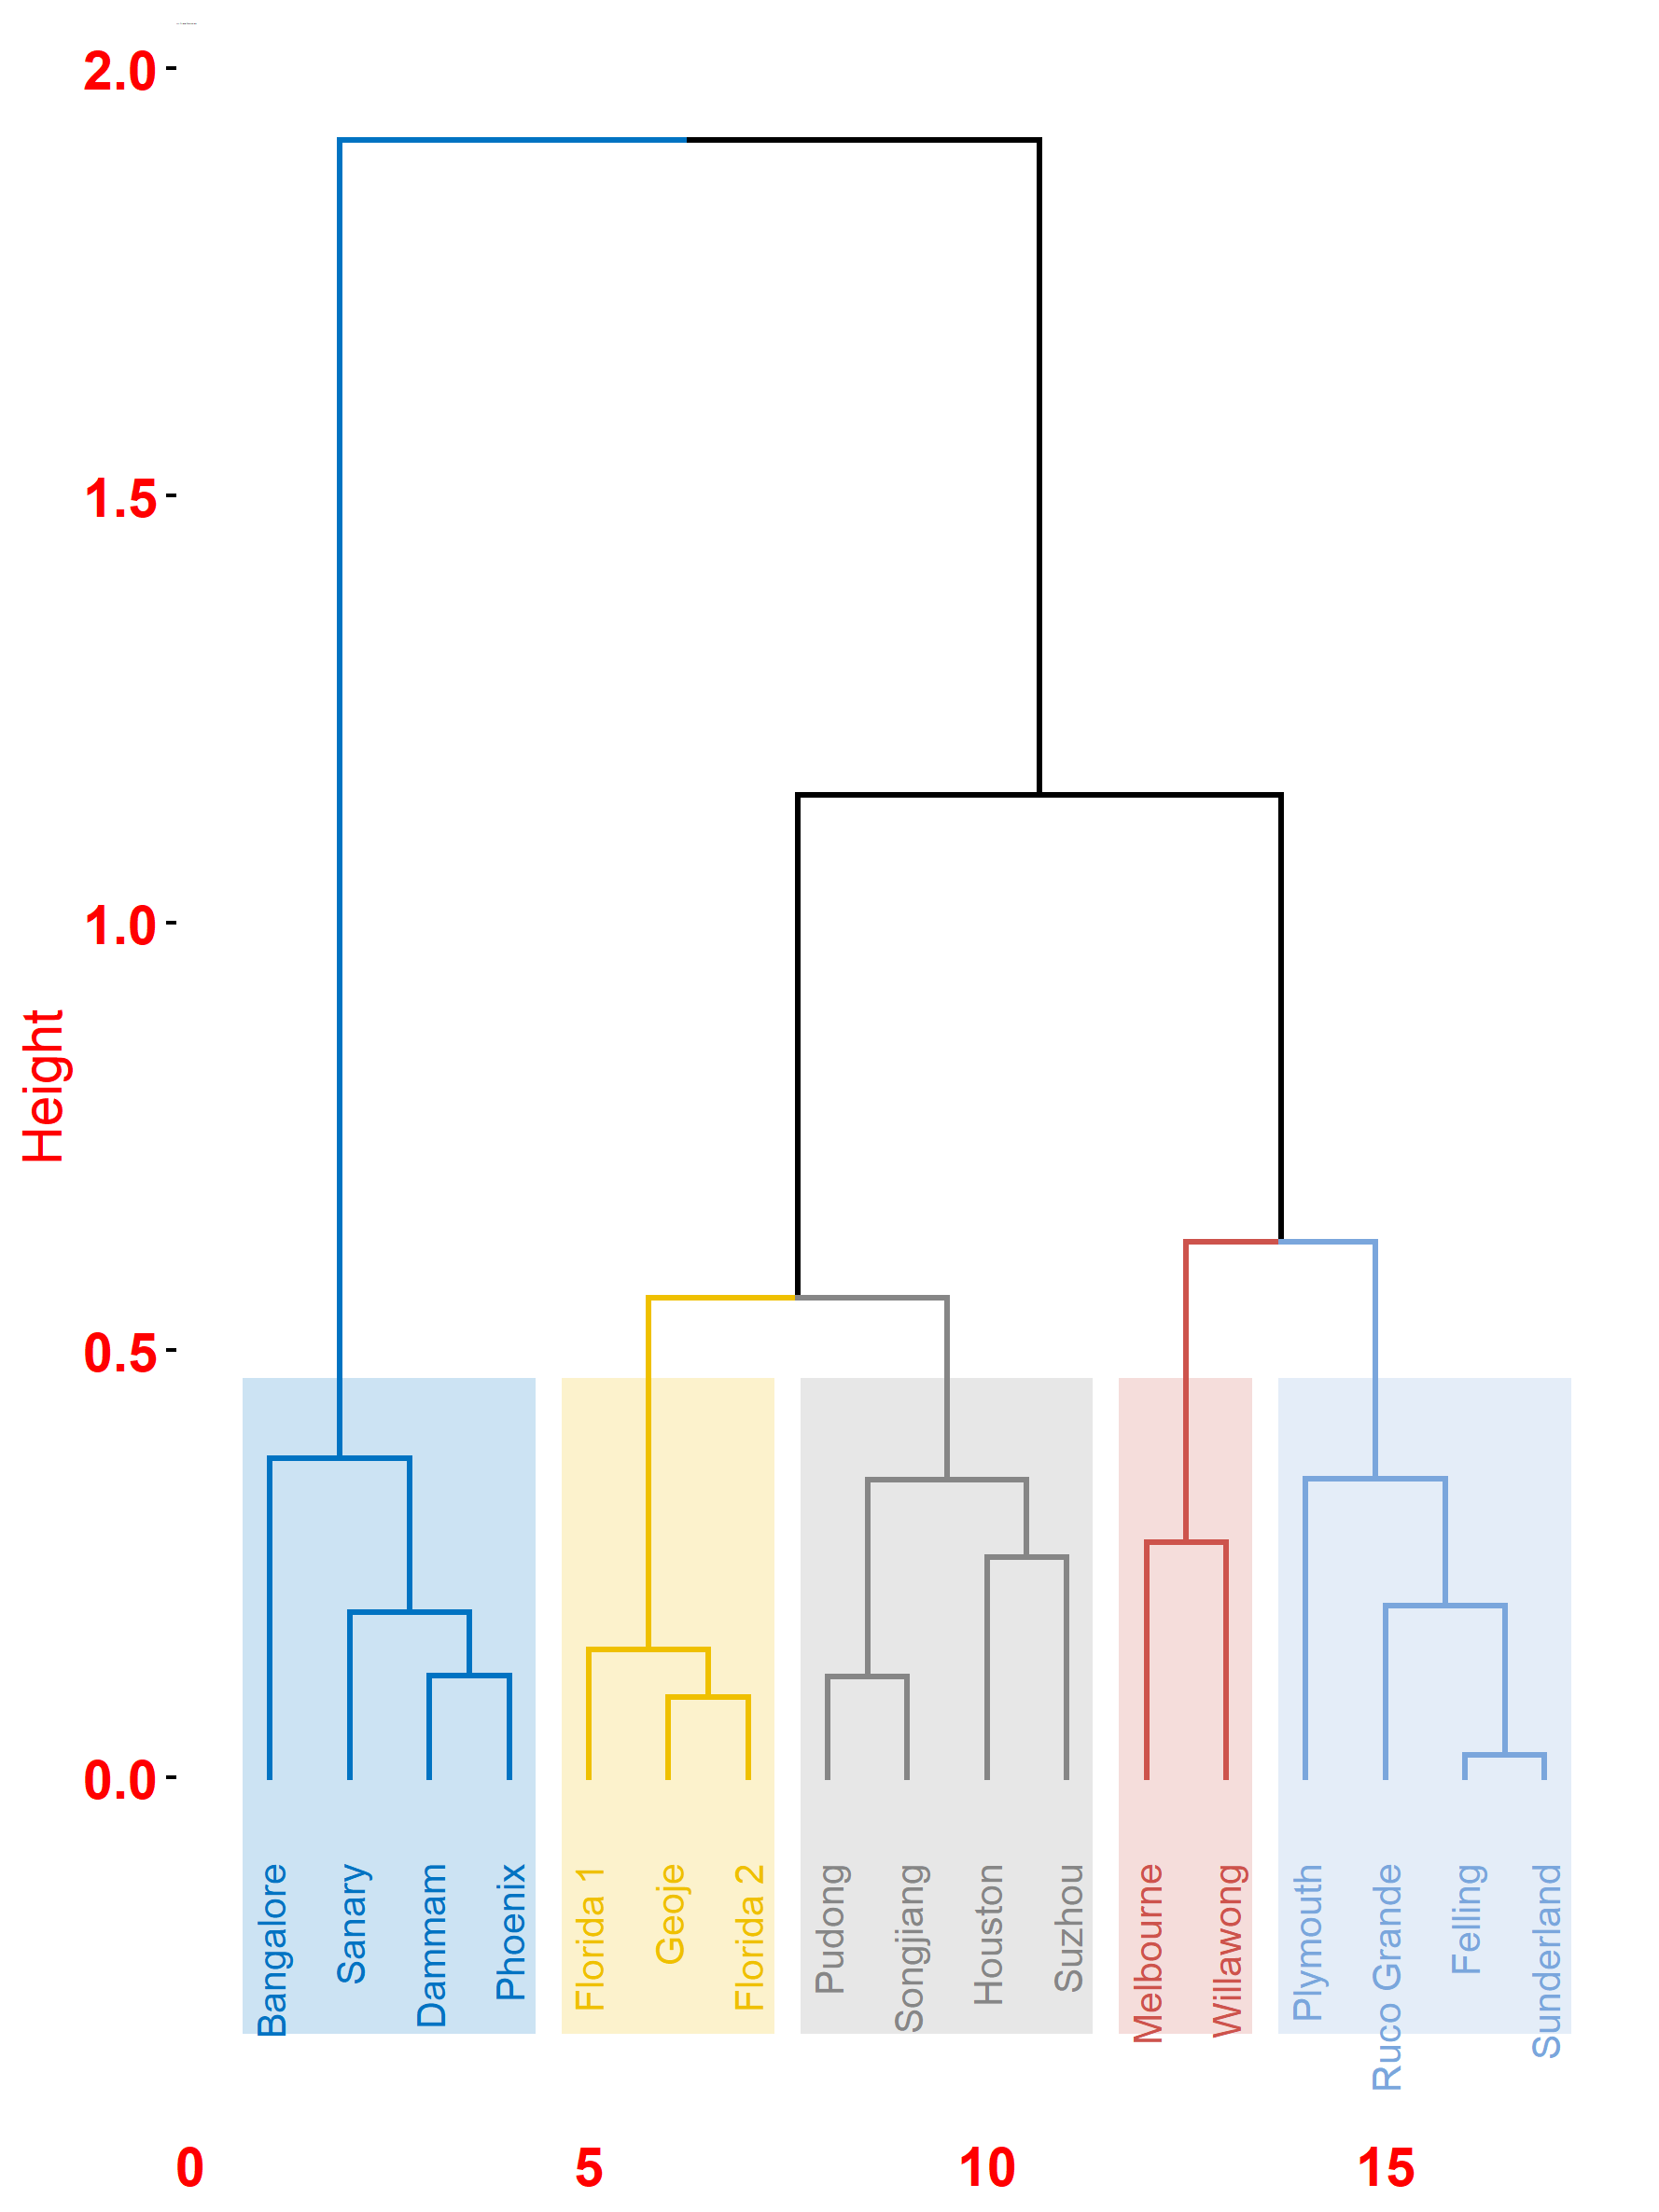
\includegraphics[width=.48\textwidth,height=6.5cm]{Jun_dend.png}}\\
\caption{Hierarchical Clustering of existing ETS for January-June}
\label{fig:jan_jun_ffp_dend}
\end{figure}

\begin{figure}[H]
\centering
\subfloat[July Hierarchical Clustering]{\label{sfig:g}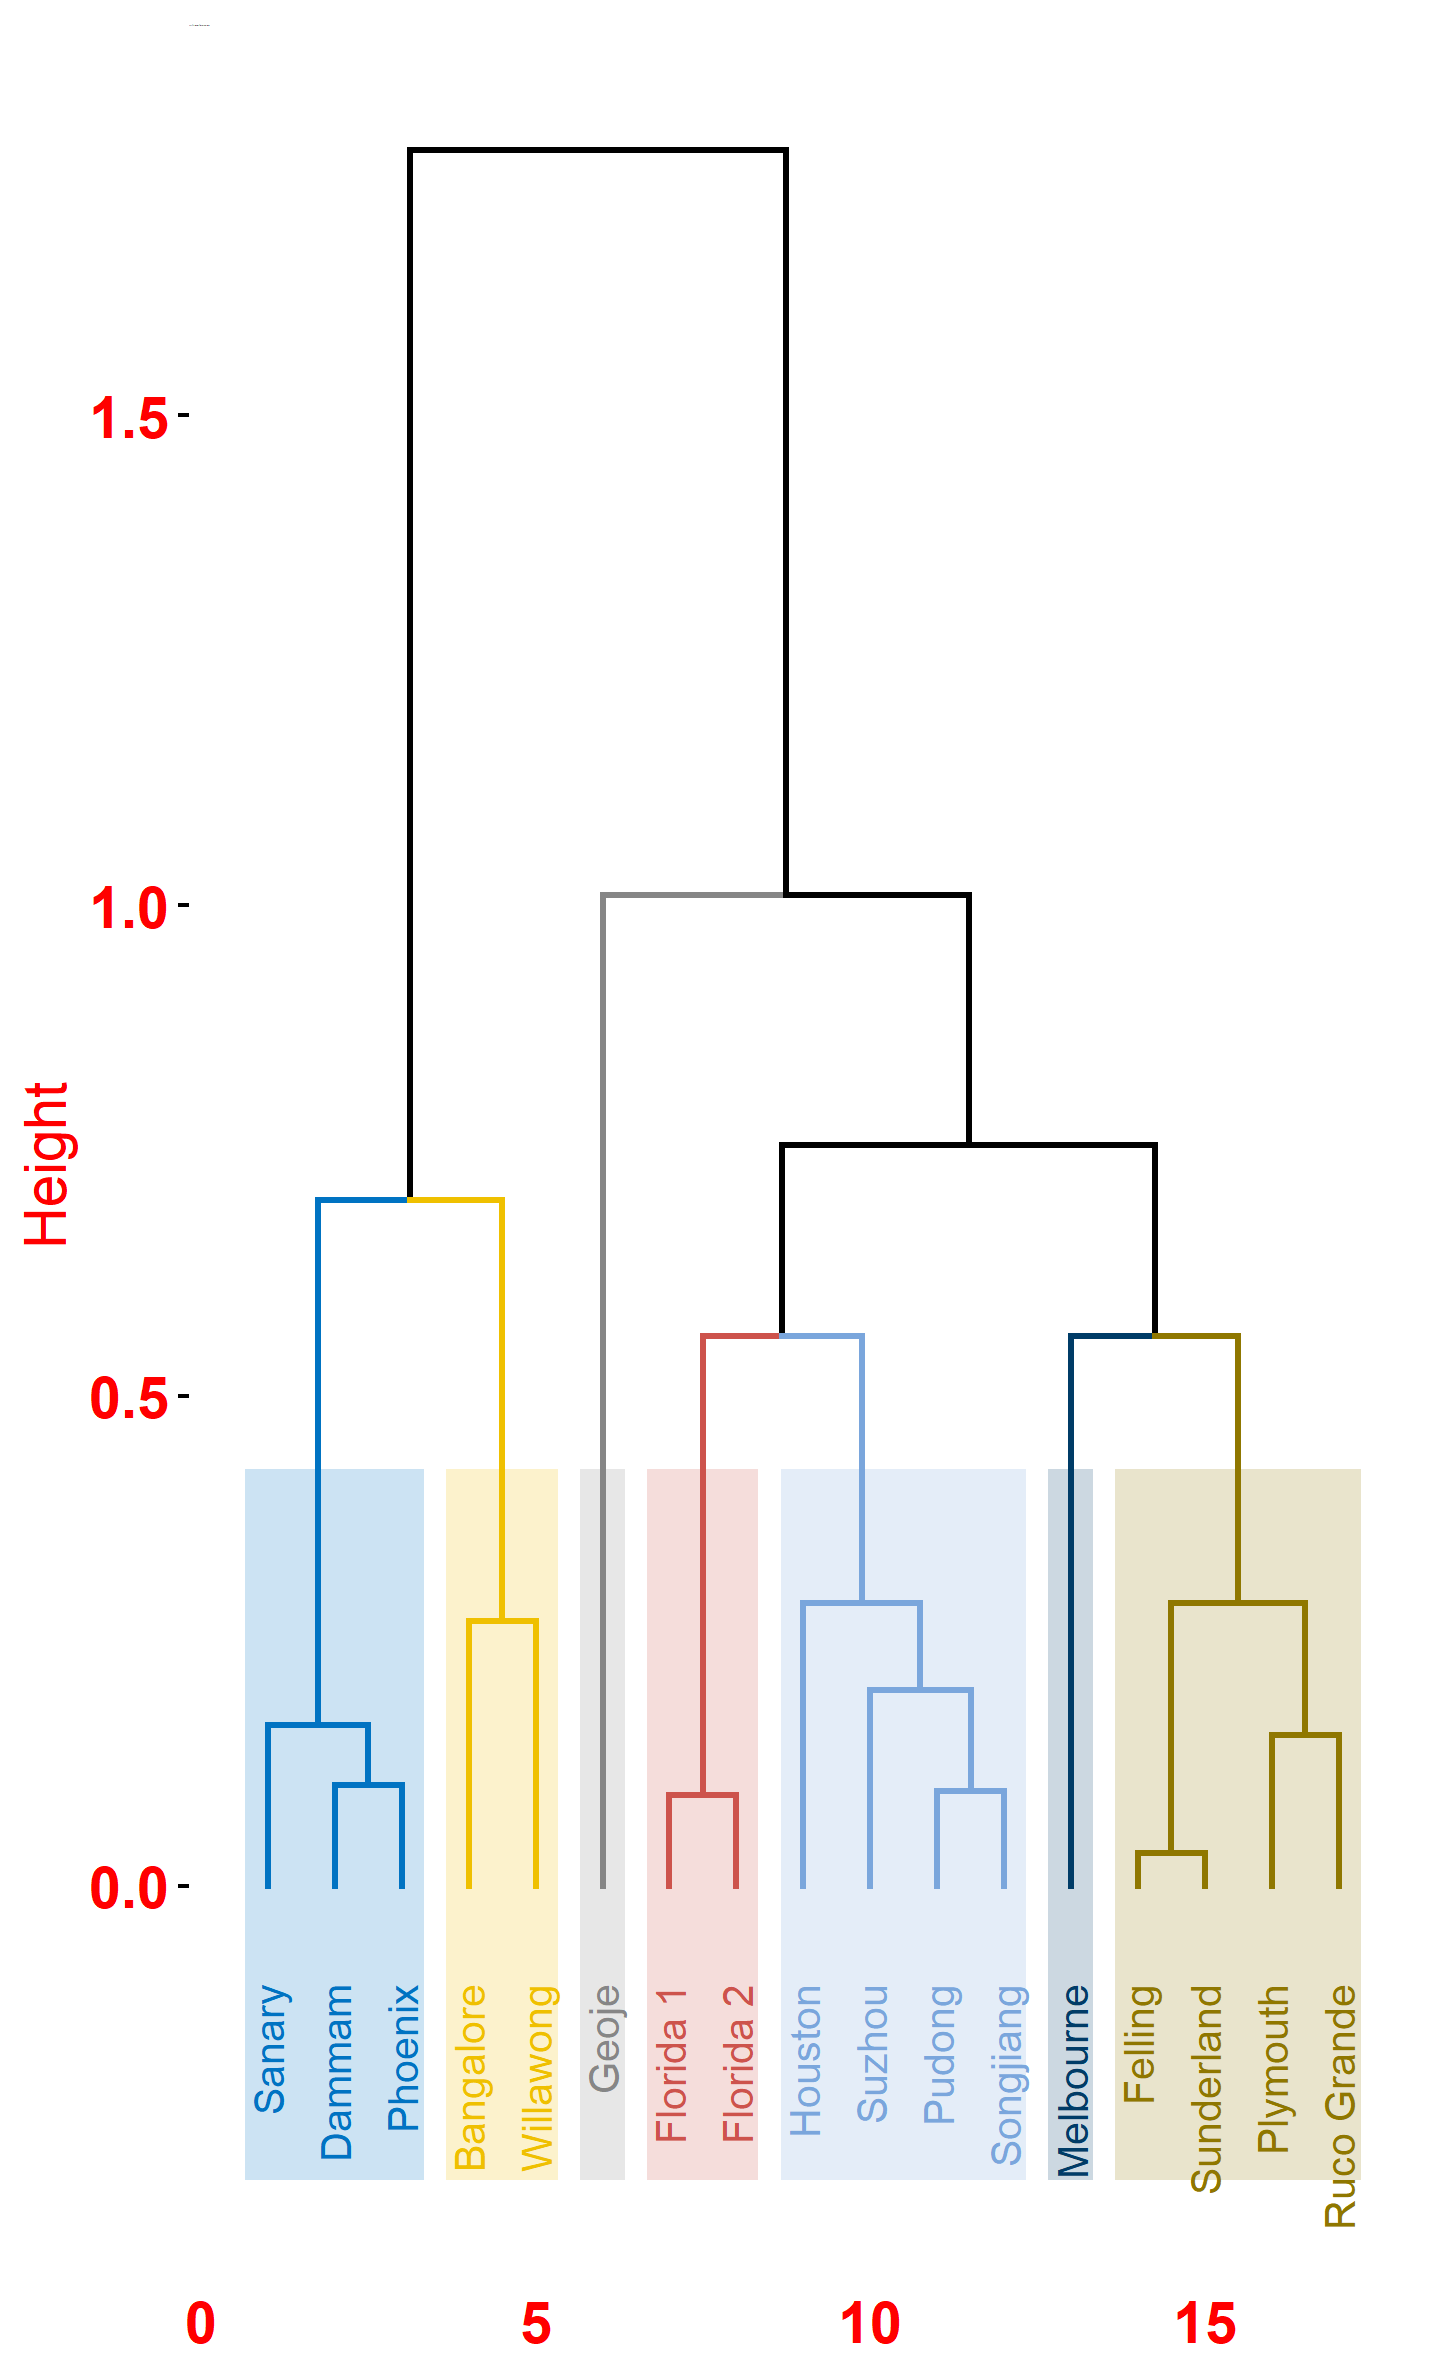
\includegraphics[width=.48\textwidth,height=6.5cm]{Jul_dend.png}}\hfill
\subfloat[August Hierarchical Clustering]{\label{sfig:h}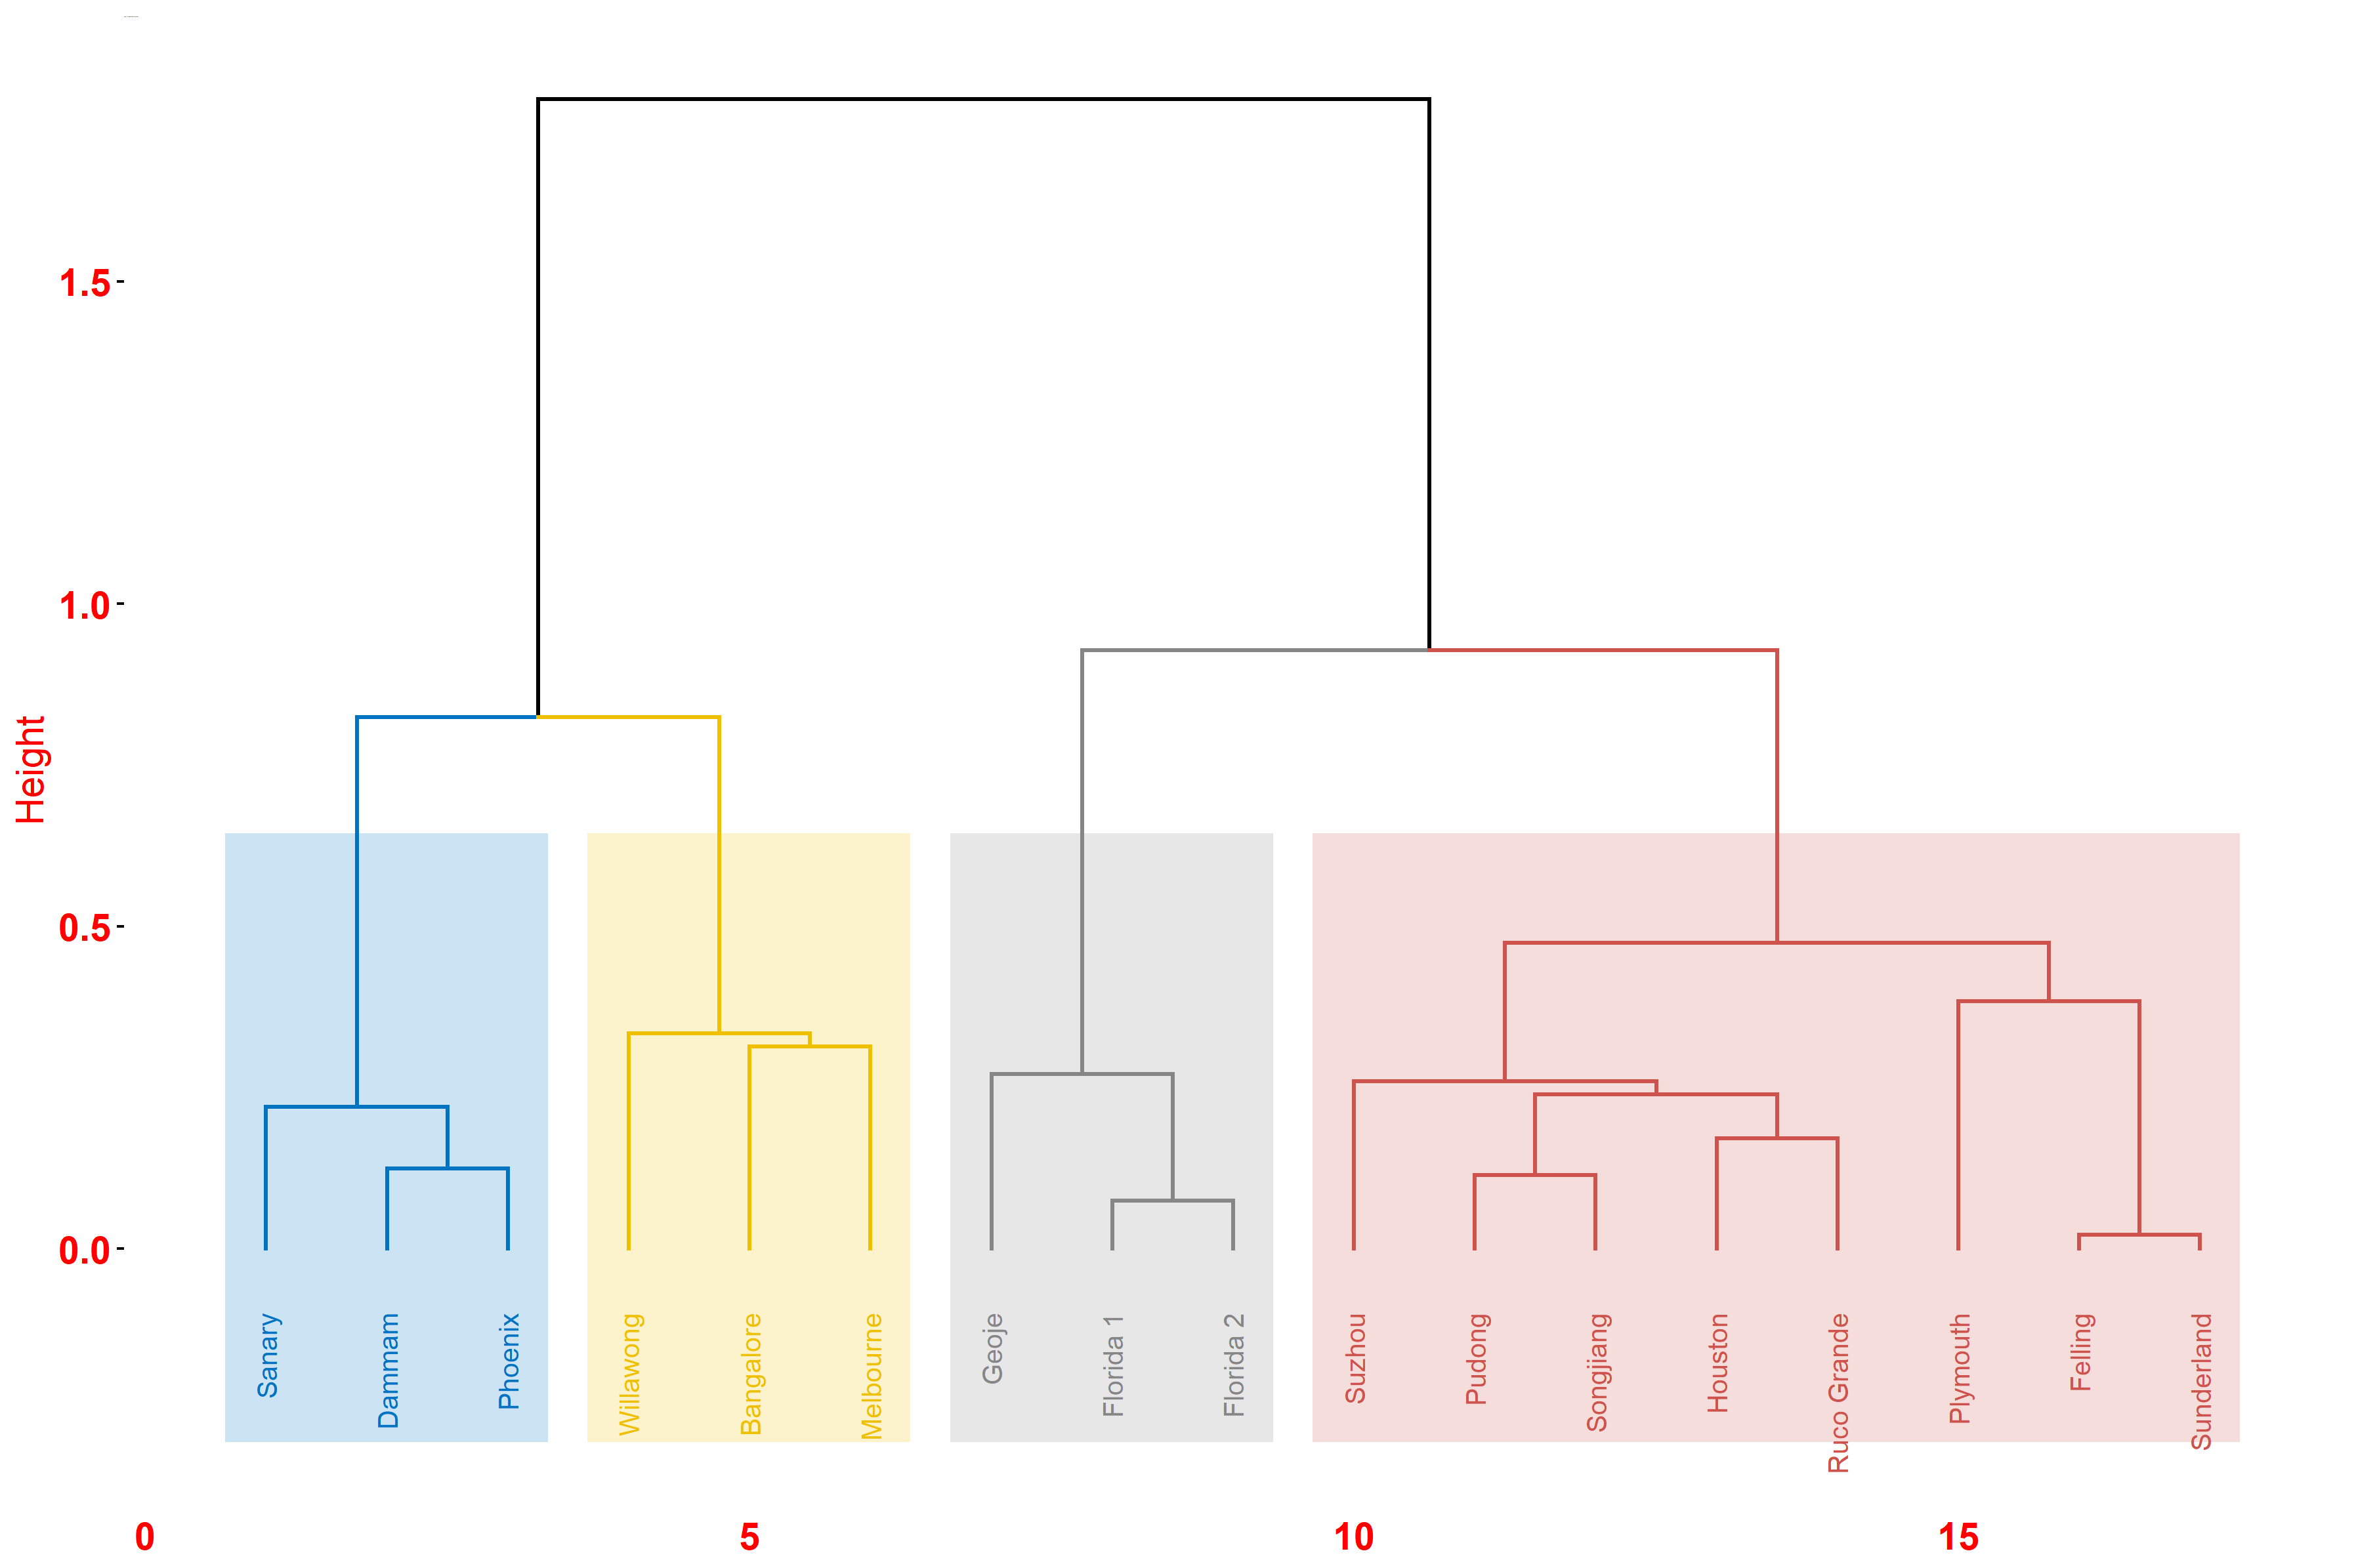
\includegraphics[width=.48\textwidth,height=6.5cm]{Aug_dend.png}}\\
\subfloat[September Hierarchical Clustering]{\label{sfig:i}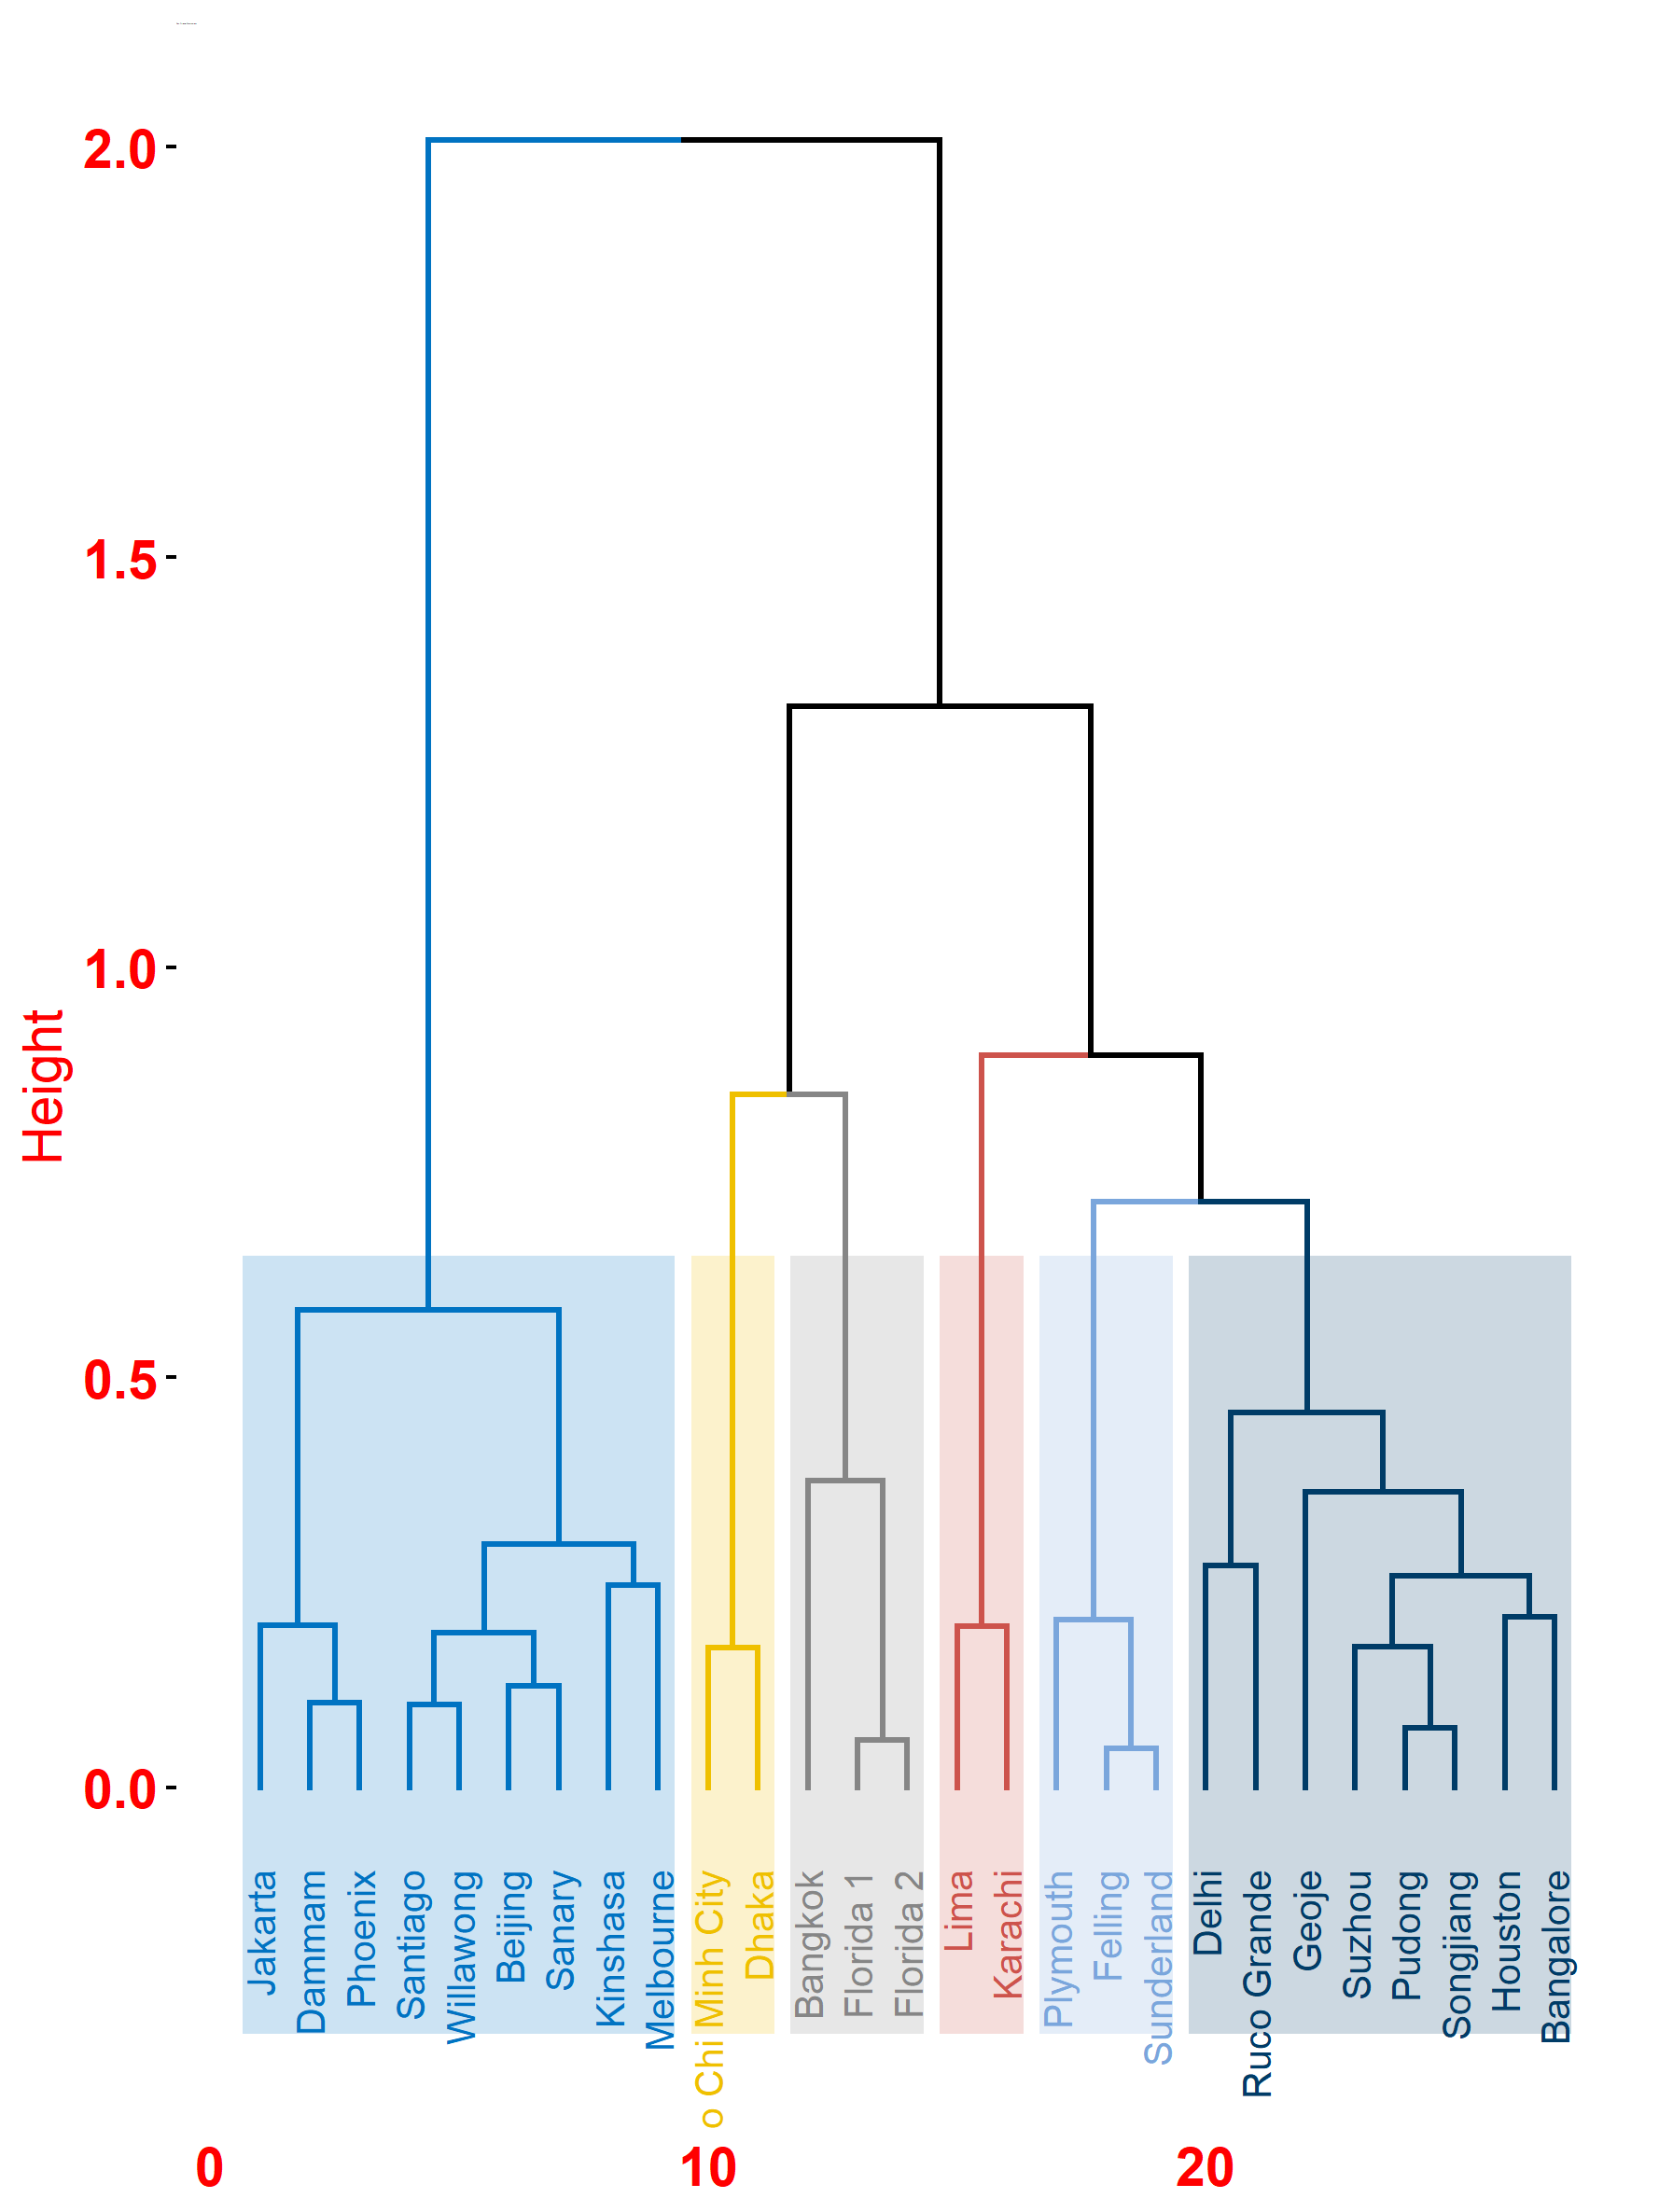
\includegraphics[width=.48\textwidth,height=6.5cm]{Sep_dend.png}}\hfill
\subfloat[October Hierarchical Clustering]{\label{sfig:j}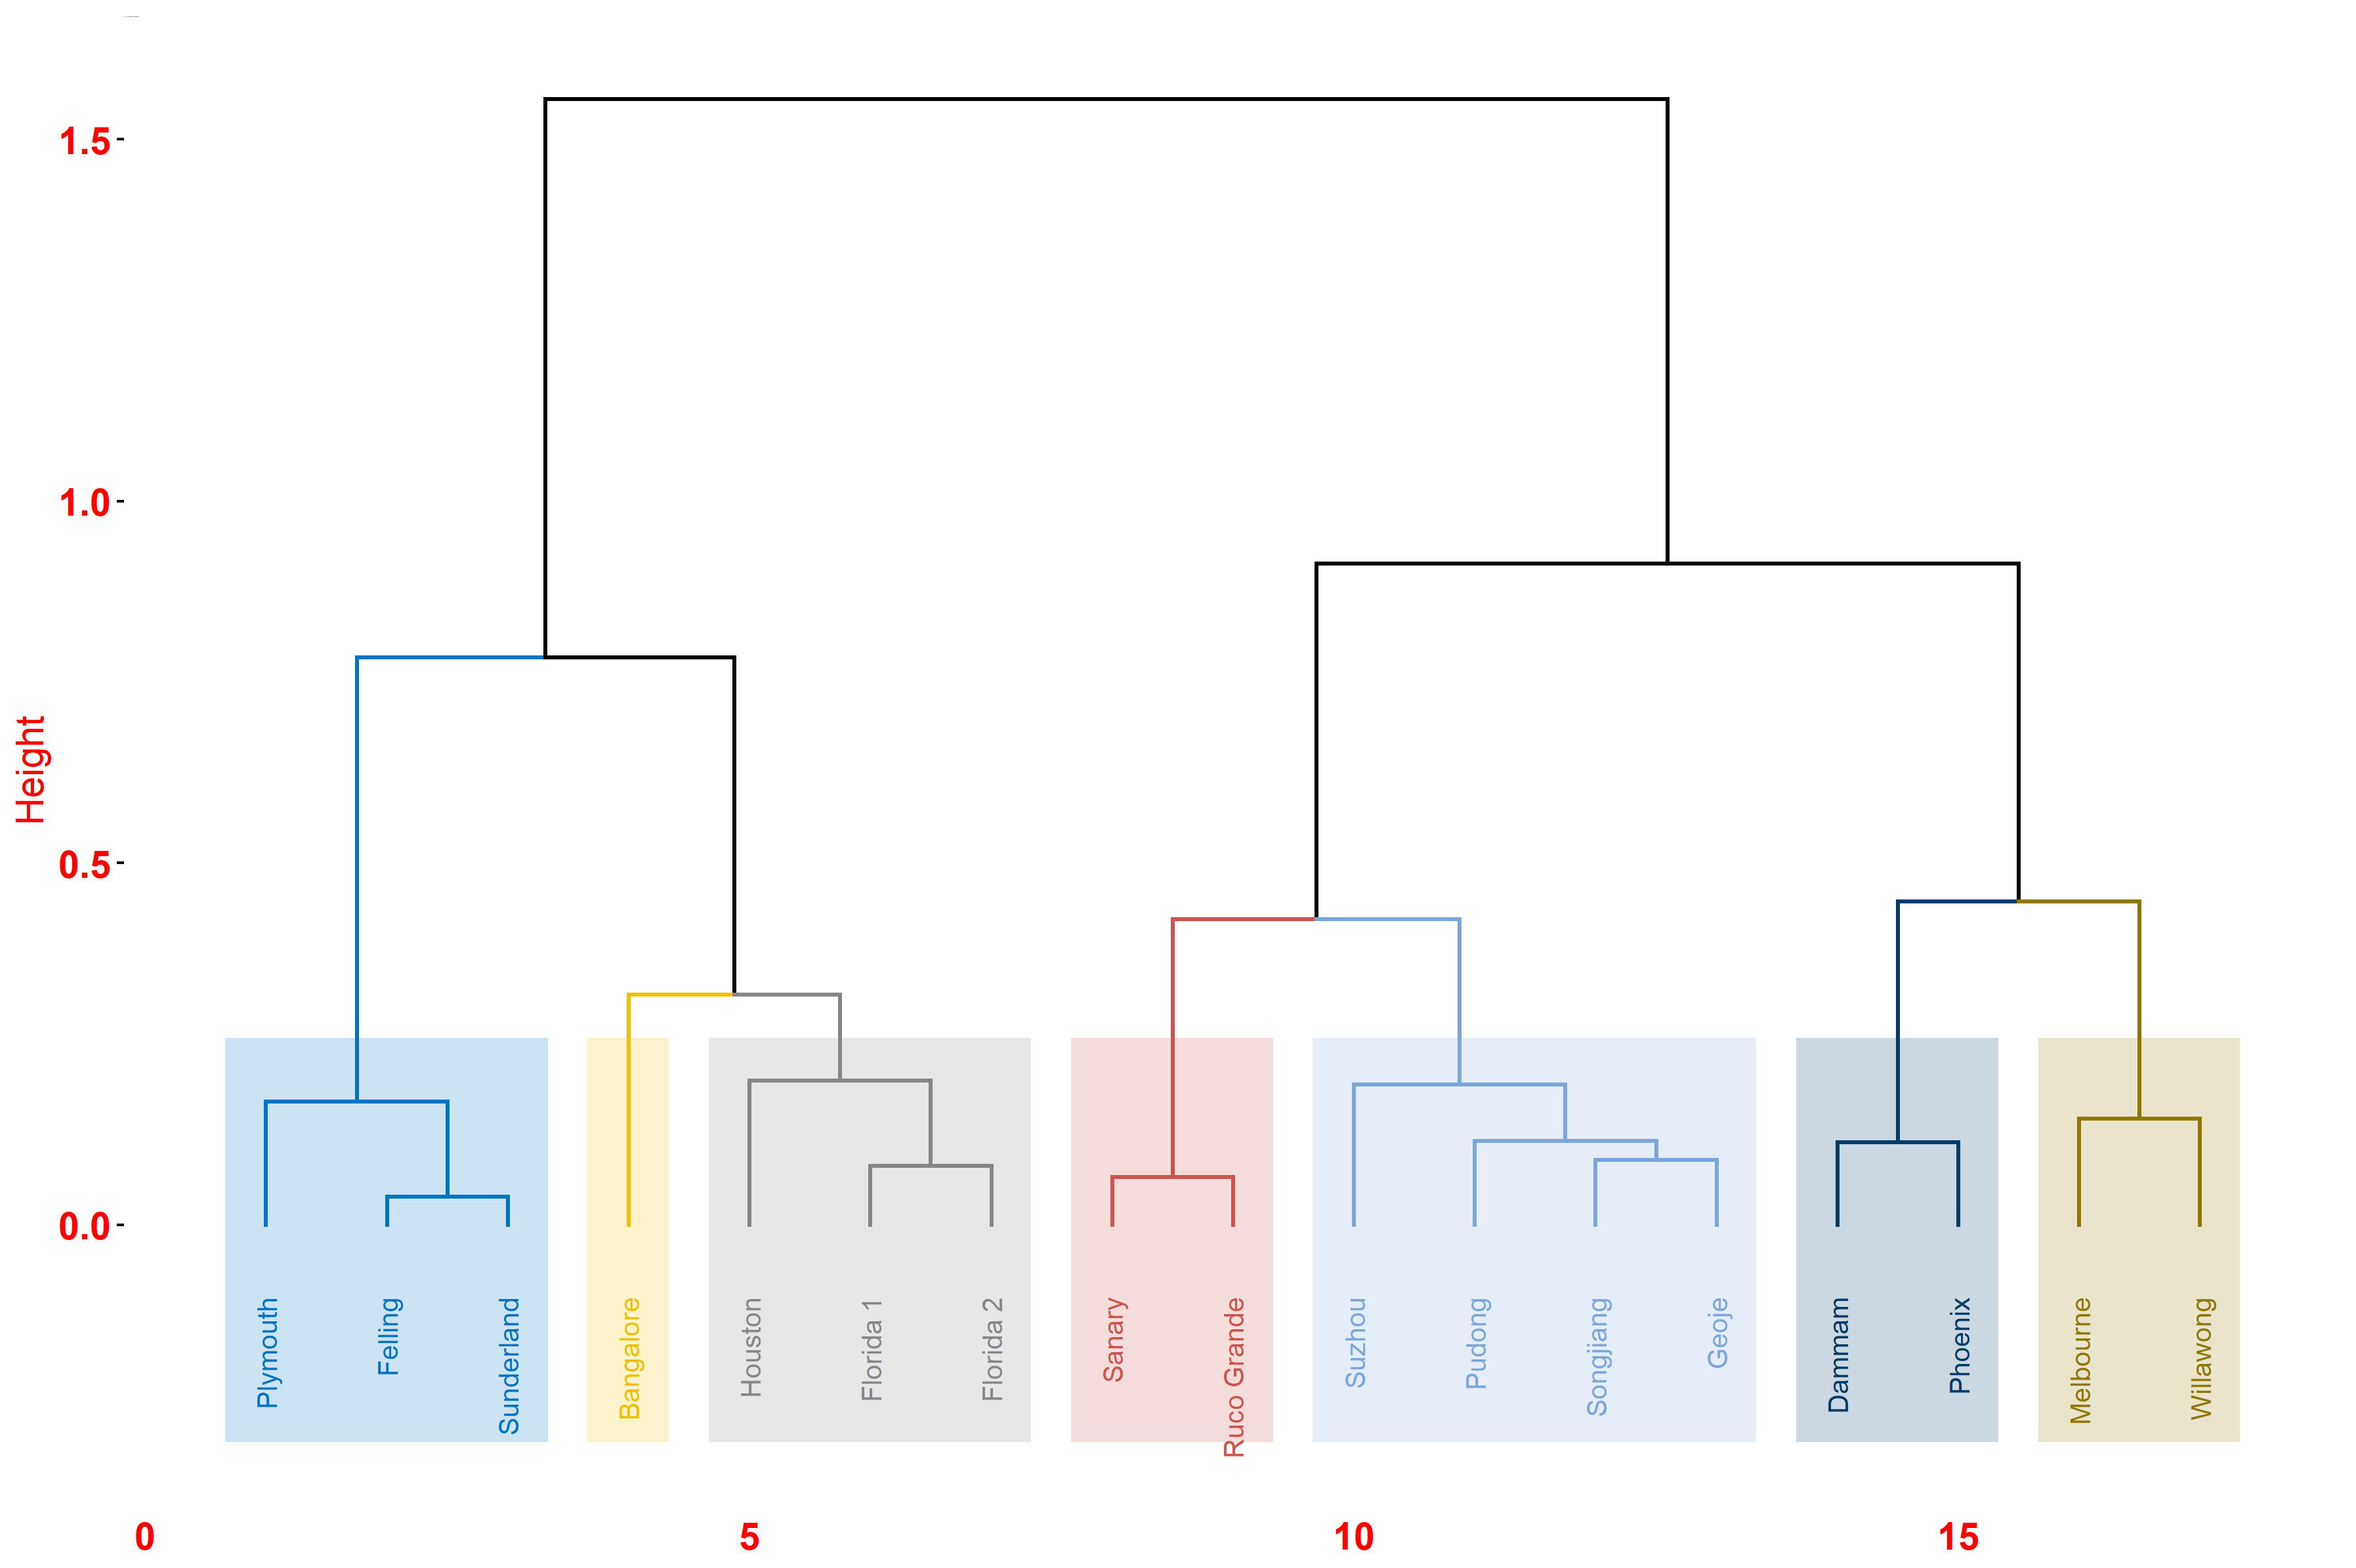
\includegraphics[width=.48\textwidth,height=6.5cm]{Oct_dend.png}}\\
\subfloat[November Hierarchical Clustering]{\label{sfig:j}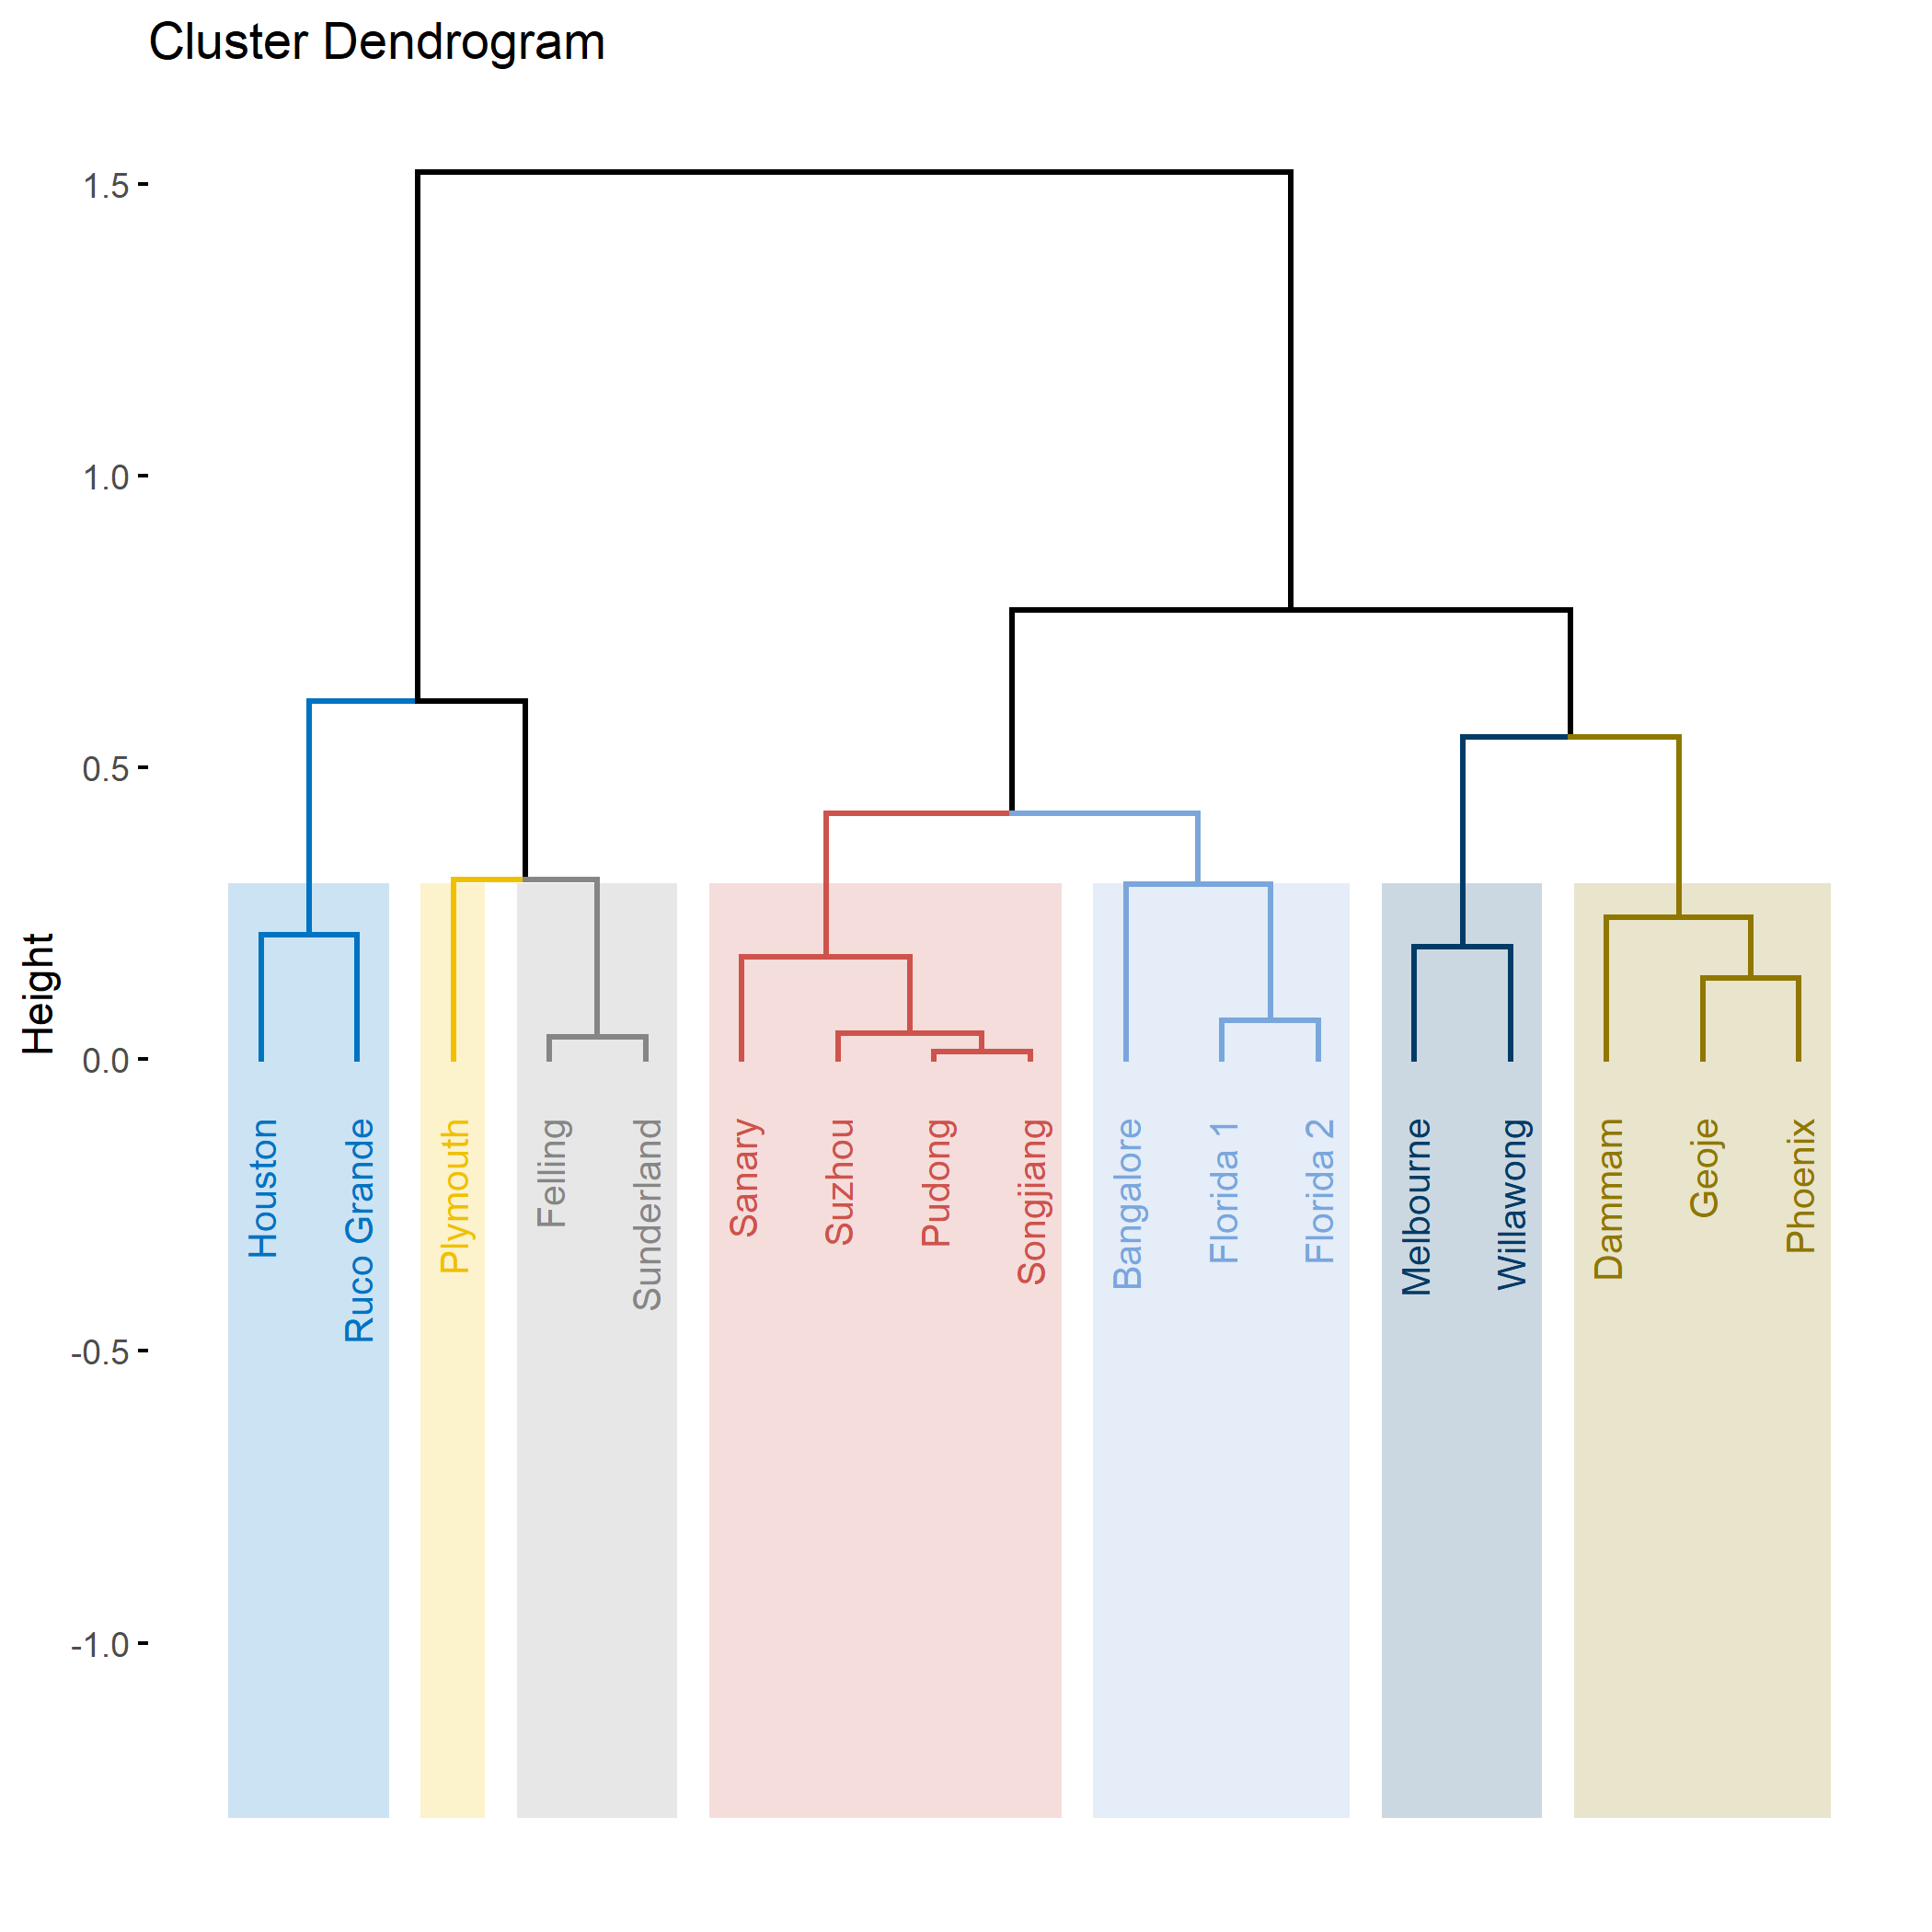
\includegraphics[width=.48\textwidth,height=6.5cm]{Nov_dend.png}}\hfill
\subfloat[December Hierarchical Clustering]{\label{sfig:j}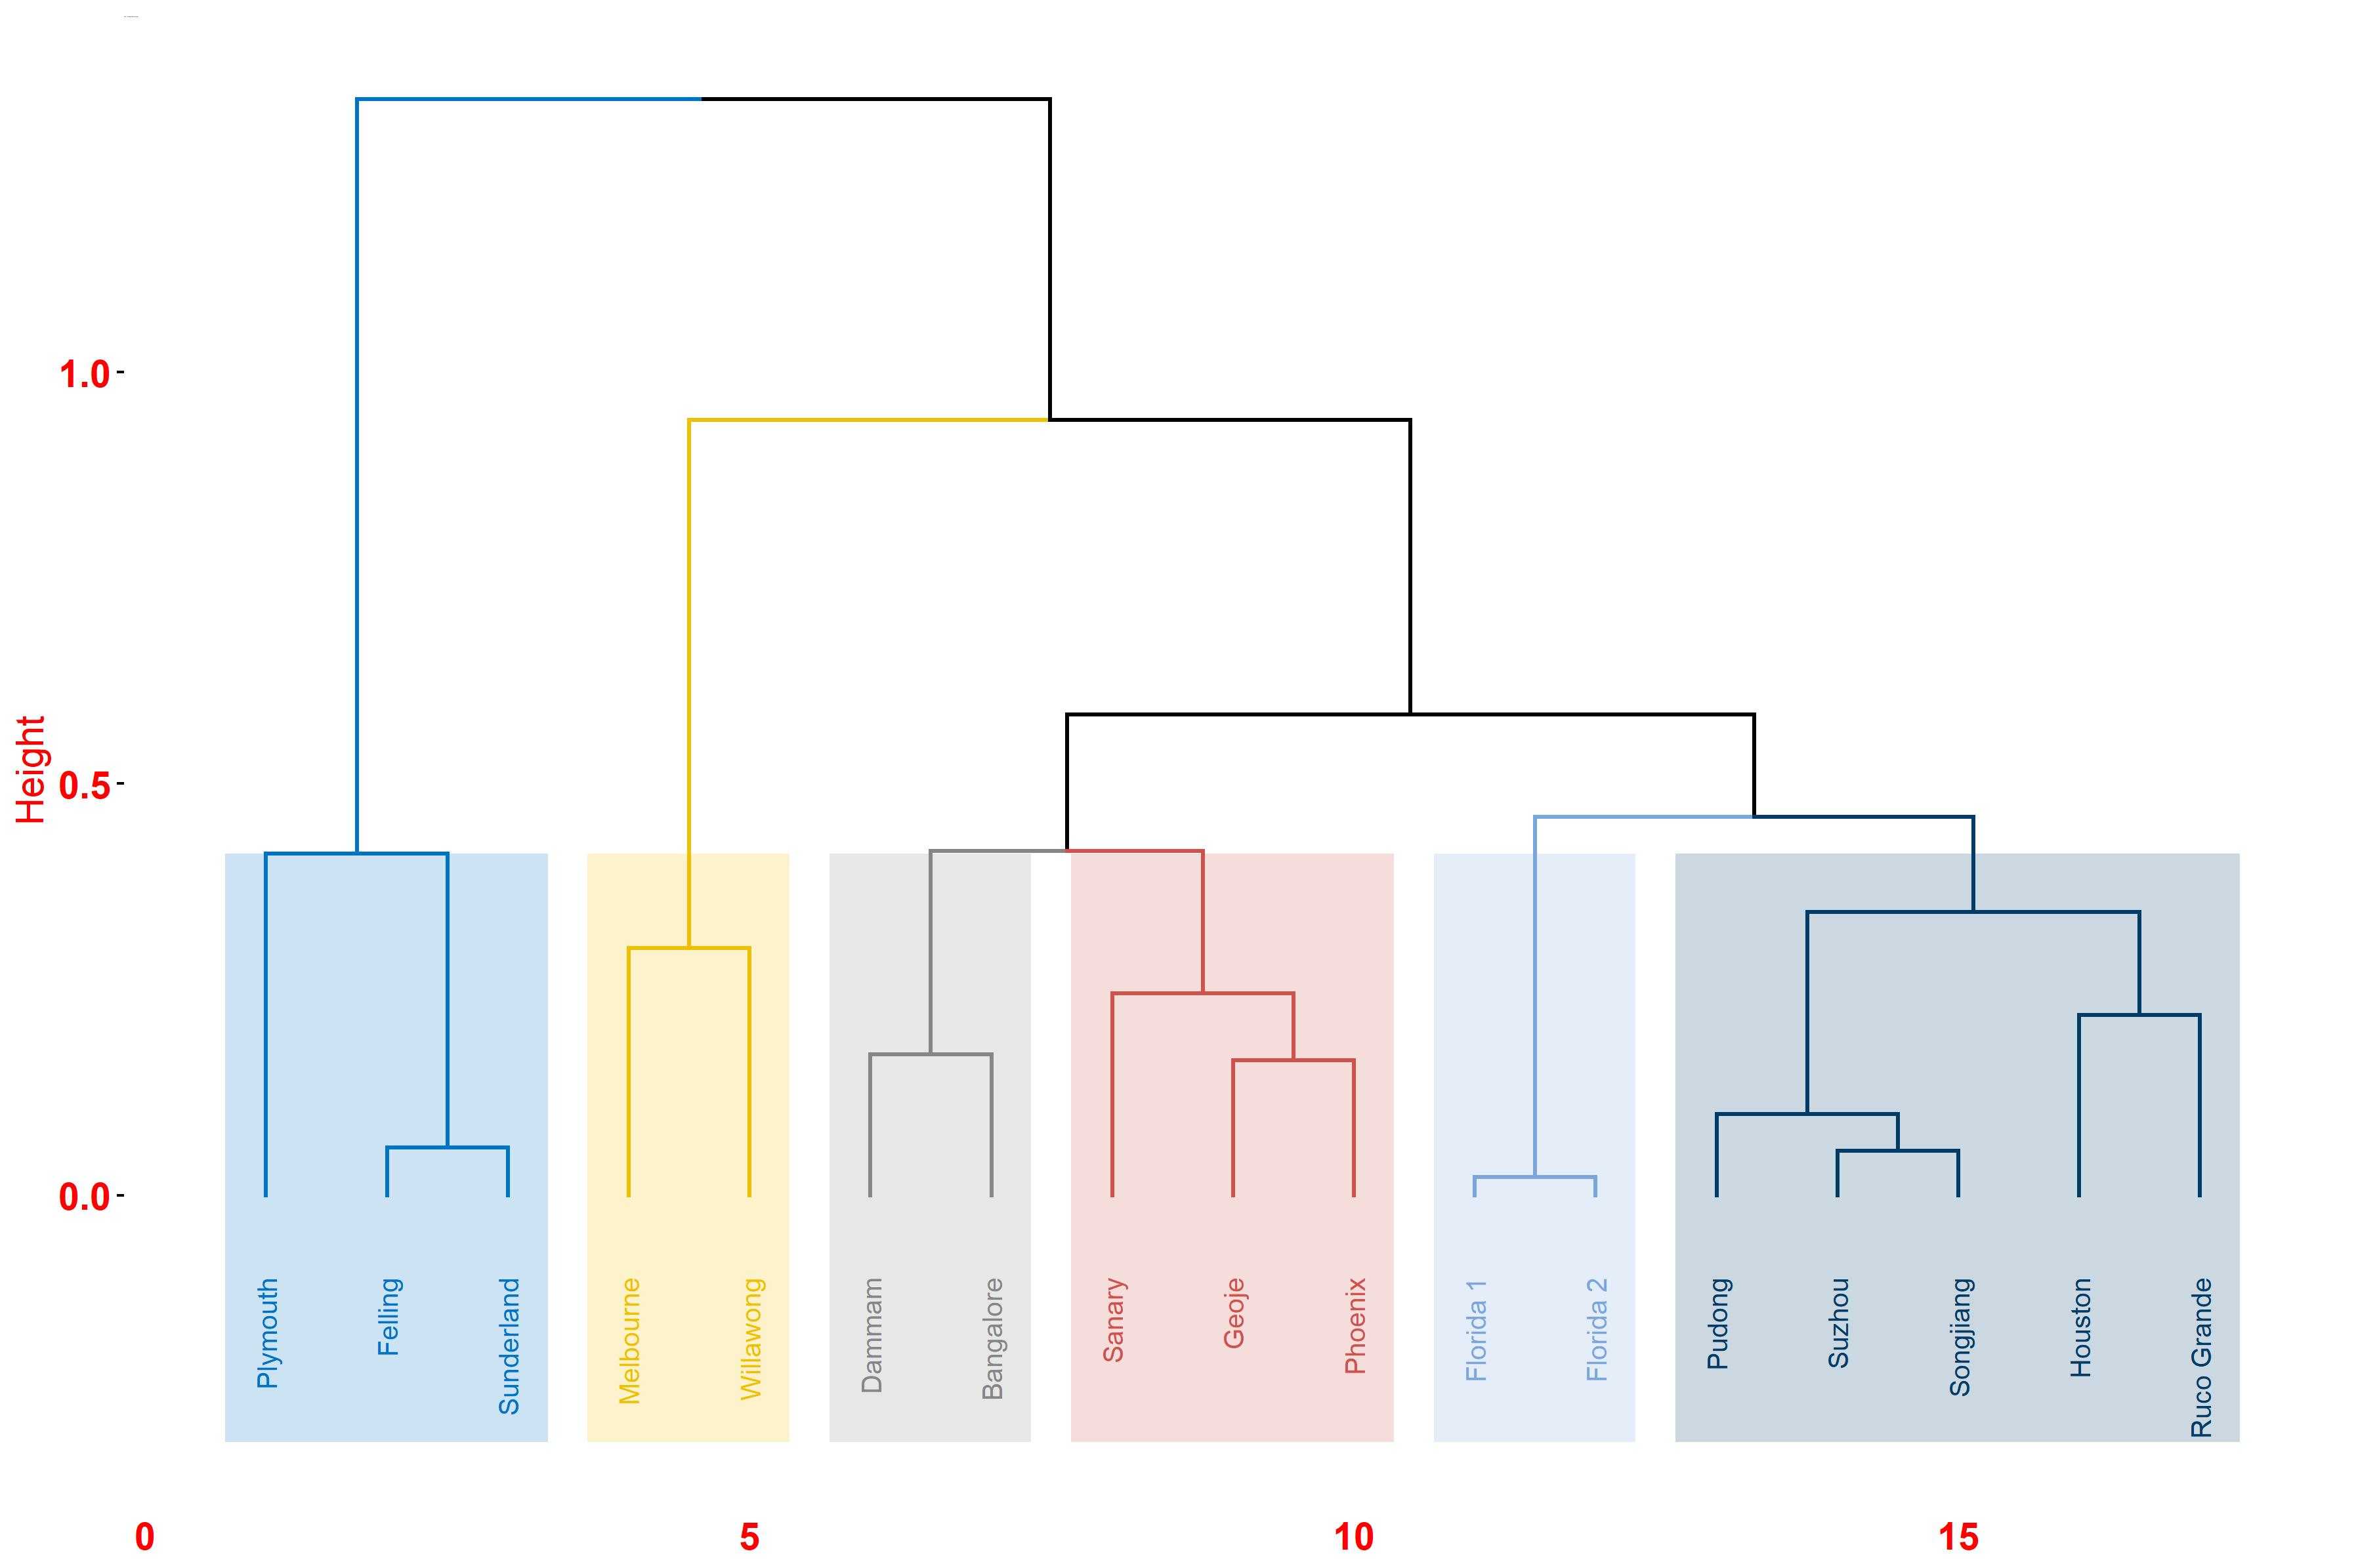
\includegraphics[width=.48\textwidth,height=6.5cm]{Dec_dend.png}}\\
\caption{HierarchicalClustering of existing ETS for July-December}
\label{fig:jul_dec_ffp_dend}
\end{figure}


Figure \ref{fig:match_matrix_ffp_pam} shows a matrix of how many times 2 locations are clustered in the same group. By considering the maximum value for each location it is possible to identify the most unique and least unique locations. Outside of the pairs mentioned above the pairings with the next highest number of times grouped in the same cluster is Suzhou and Pudong,  Suzhou and Songjiang, Felling and Plymouth, Sunderland and Plymouth with 11 months in the same cluster, again these parings are intuitively obvious due to the close geographical proximity. 

\begin{figure}[H]
\centering
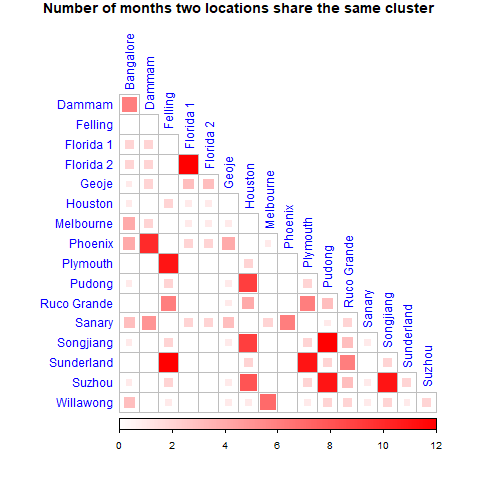
\includegraphics[width=0.6\textwidth]{match_matrix_ffp_pam.png}
\caption{Matrix of the number of times two locations are grouped in the same cluster}
\label{fig:match_matrix_ffp_pam}
\end{figure}




Figure \ref{fig:var_means_ffp} shows the percentage difference of the annual mean value for each variable for a given location when compared to the annual mean value of the whole data set. These statistics will be used to characterise each locations environment and identify in the empirical data what makes locations similar and different. 

\begin{figure}[H]
\centering
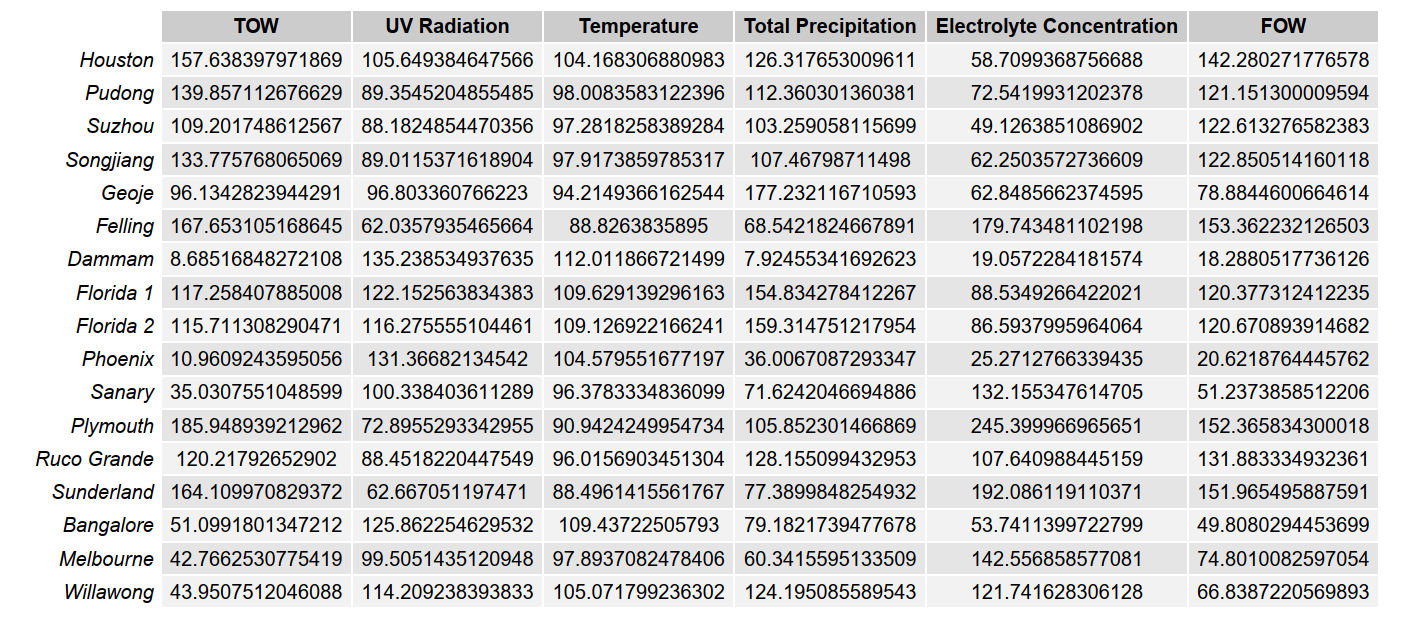
\includegraphics[width=0.9\textwidth, height= 6cm]{variable_means_ffp.png}
\caption{Percentage difference of annual mean for each location when compared to the annual mean for the entire data set}
\label{fig:var_means_ffp}
\end{figure}


Dammam and Phoenix have 10 months when clustered in the same group. The climate in these locations is a desert climate with low precipitation and high temperatures. It is clear from figure \ref{fig:var_means_ffp} that Dammam and Phoenix are characterised by significantly lower TOW, FOW, Precipiration and concentration of electrolyte when compared to the whole data set. The UV radiation level is also significantly higher than the mean for the data set.     

Houston shares clusters with Pudong and Songjiang for 9 months and with Suzhou for 8 months, the climate in all of these locations is warm  with significant rainfall. Figure \ref{fig:var_means_ffp} shows that these locations have significantly higher TOW, FOW and lesser values of electrolyte concentration. Temperature and UV values are closer to the mean of the data set.  

Melbourne and Willawong share the same cluster for 7 months of the year. The climate of these locations is characterised by low values for TOW and FOW and high values for concentration of electrolyte. However, these two locations differ in precipitation values, Willawong has significantly above average precipitation and Melbourne has significantly below average precipitation values. This might explain why the two locations are only clustered 7 times together. For 5 months of the year Melbourne is not clustered with any other locations, this suggests it is an outlier in the data set and one of the most unique ETS available to AkzoNobel.

Outside of these parings no two locations share more than 6 months in the same cluster. The fact that these locations are only clustered together for half of a year suggest significant difference in the monthly climate of these locations. When compared to other ETS in this analysis Geoje, Sanary, Ruco Grande and Bangalore all have unique climates. 

Geoje is characterised by the highes precipitation values in the data set and electrolyte concentration values significantly below the data set mean. The FOw for Geoje is also lower than the data set mean, this is unusual for a location with high precipitation values, only Willawong shares this characteristic. Geoje is left as an outlier in clustering on two occasions, in September and July, this futher confirms the uniqueness of the climate of Geoje as an ETS. 

Sanary is characterised by high concentration of electrolyte, and low TOW and FOW values. Although Sanary is never clustered with anothe location more than 6 times it is never left as an outlier in clustering, this means that the climate in Sanary could be covered by exposure testing carried out in more than one location.

Ruco Grande is characterised by slightly elevated values of TOW, FOW and Precipitation with Temperature, UV and electrolyte concentration nearer to the data set mean. Again, Ruco Grande is never an outlier in clustering and is therfore not as unique as other locations. 

Bangalore is characterised by very low values of TOW, FOW,  however,  precipitation values are closer to the mean. This can be explained by the seasonality in Bangalore consisting of Summer, Winter and Monsoon seasons. Above average precipitation values in the Monsoon seasons will bring the average for the location closer to the mean but relatively dry periods in Summer and Winter will decrease the TWO and FOW values. UV values are slightly elevated in Bangalore. Bangalore is not clustered with any locations in October.





\begin{figure}[h]
\centering
\subfloat[January PAM Clustering]{\label{sfig:a}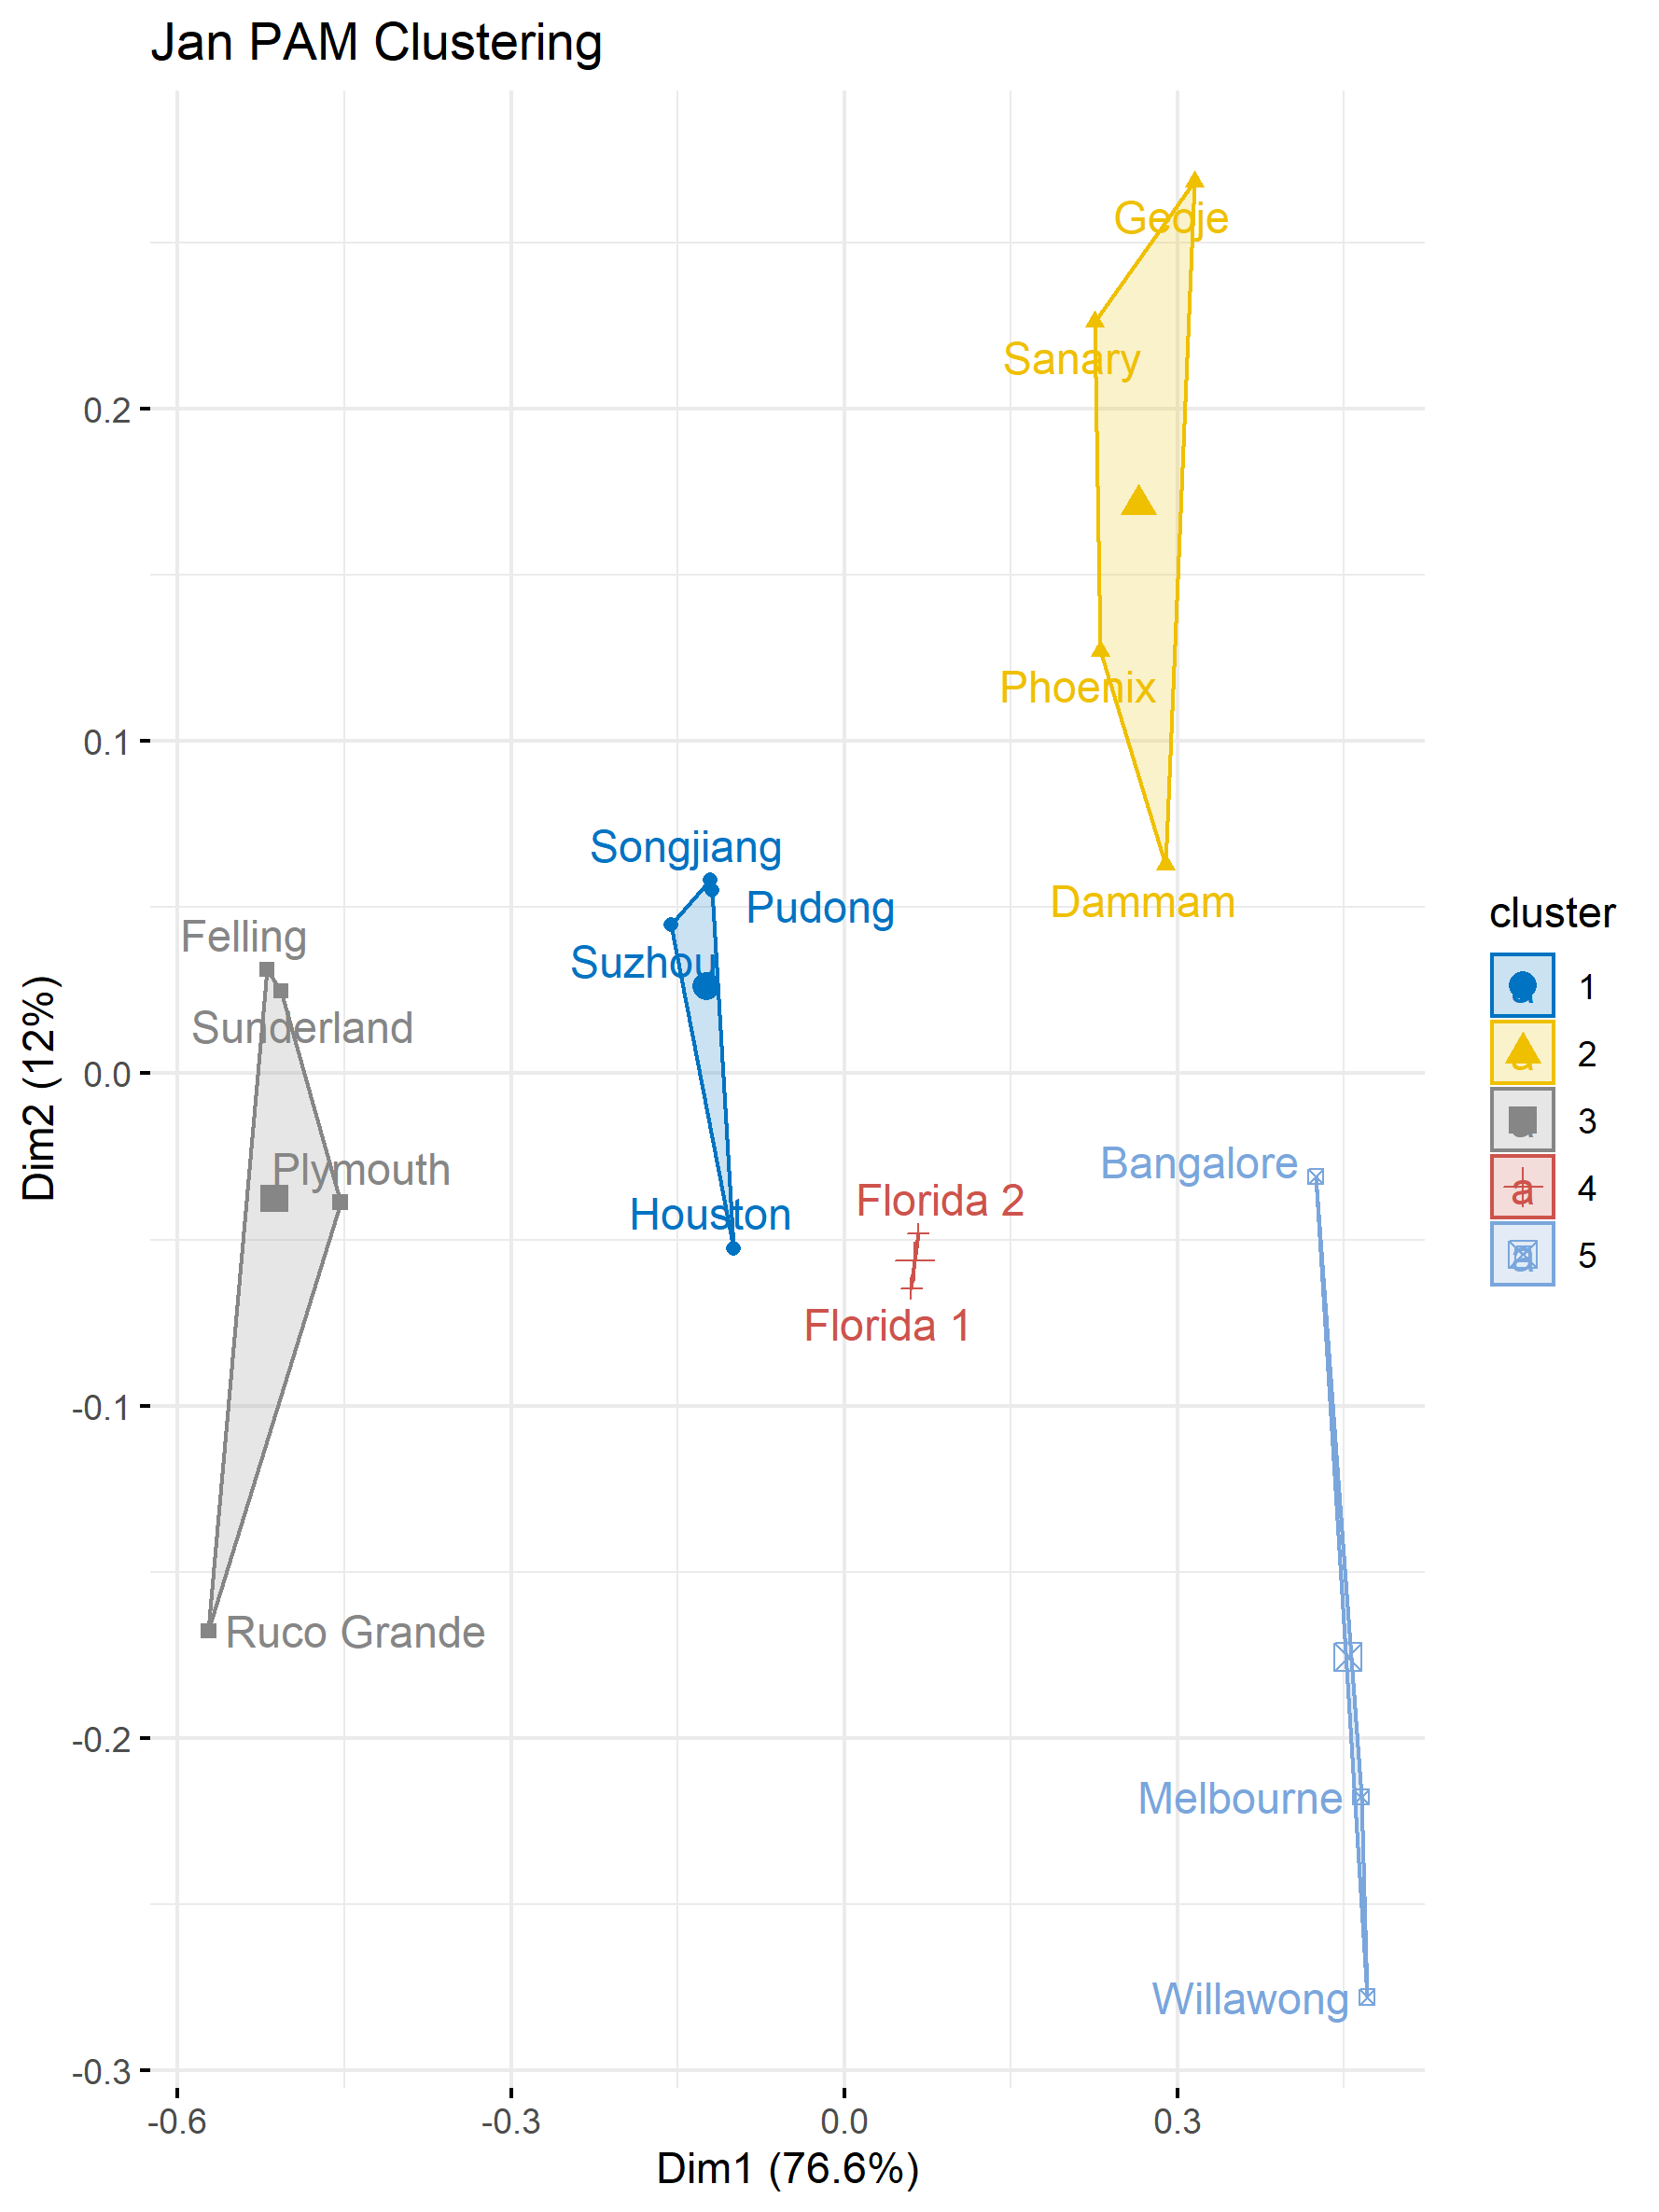
\includegraphics[width=.48\textwidth,height=6.5cm]{Jan_cluster.png}}\hfill
\subfloat[February PAM Clustering]{\label{sfig:b}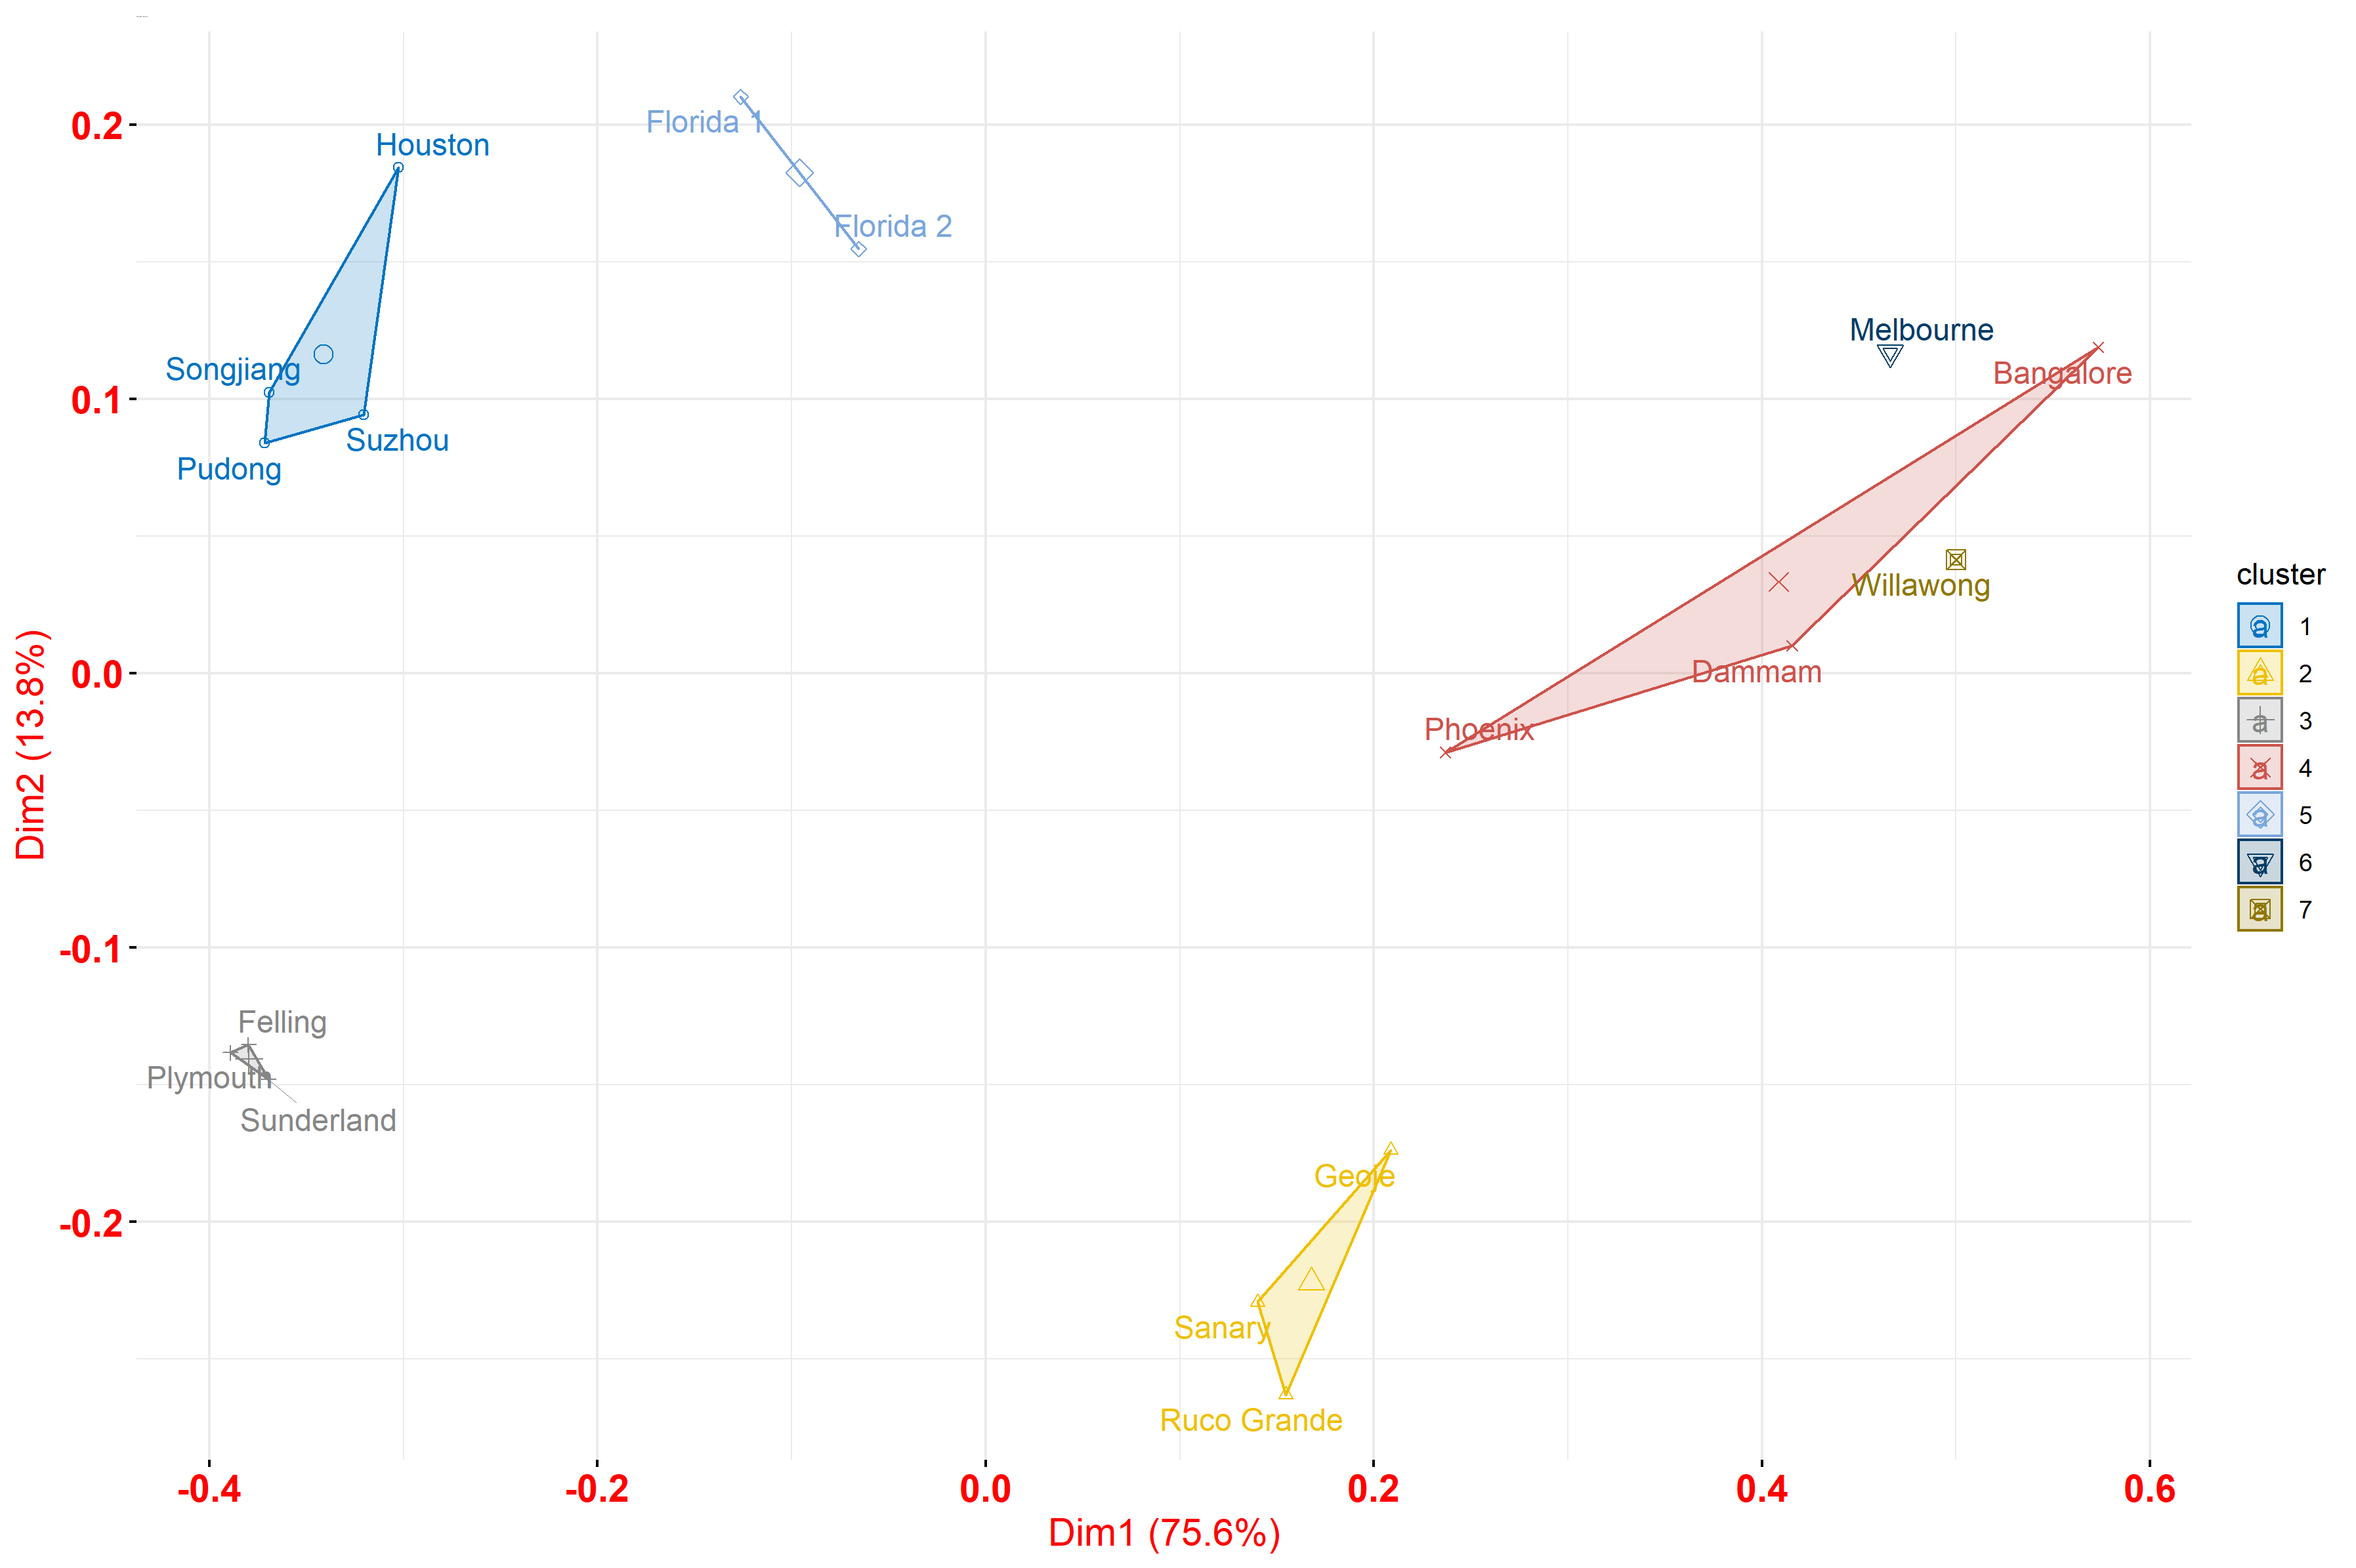
\includegraphics[width=.48\textwidth,height=6.5cm]{Feb_cluster.png}}\\
\subfloat[March PAM Clustering]{\label{sfig:c}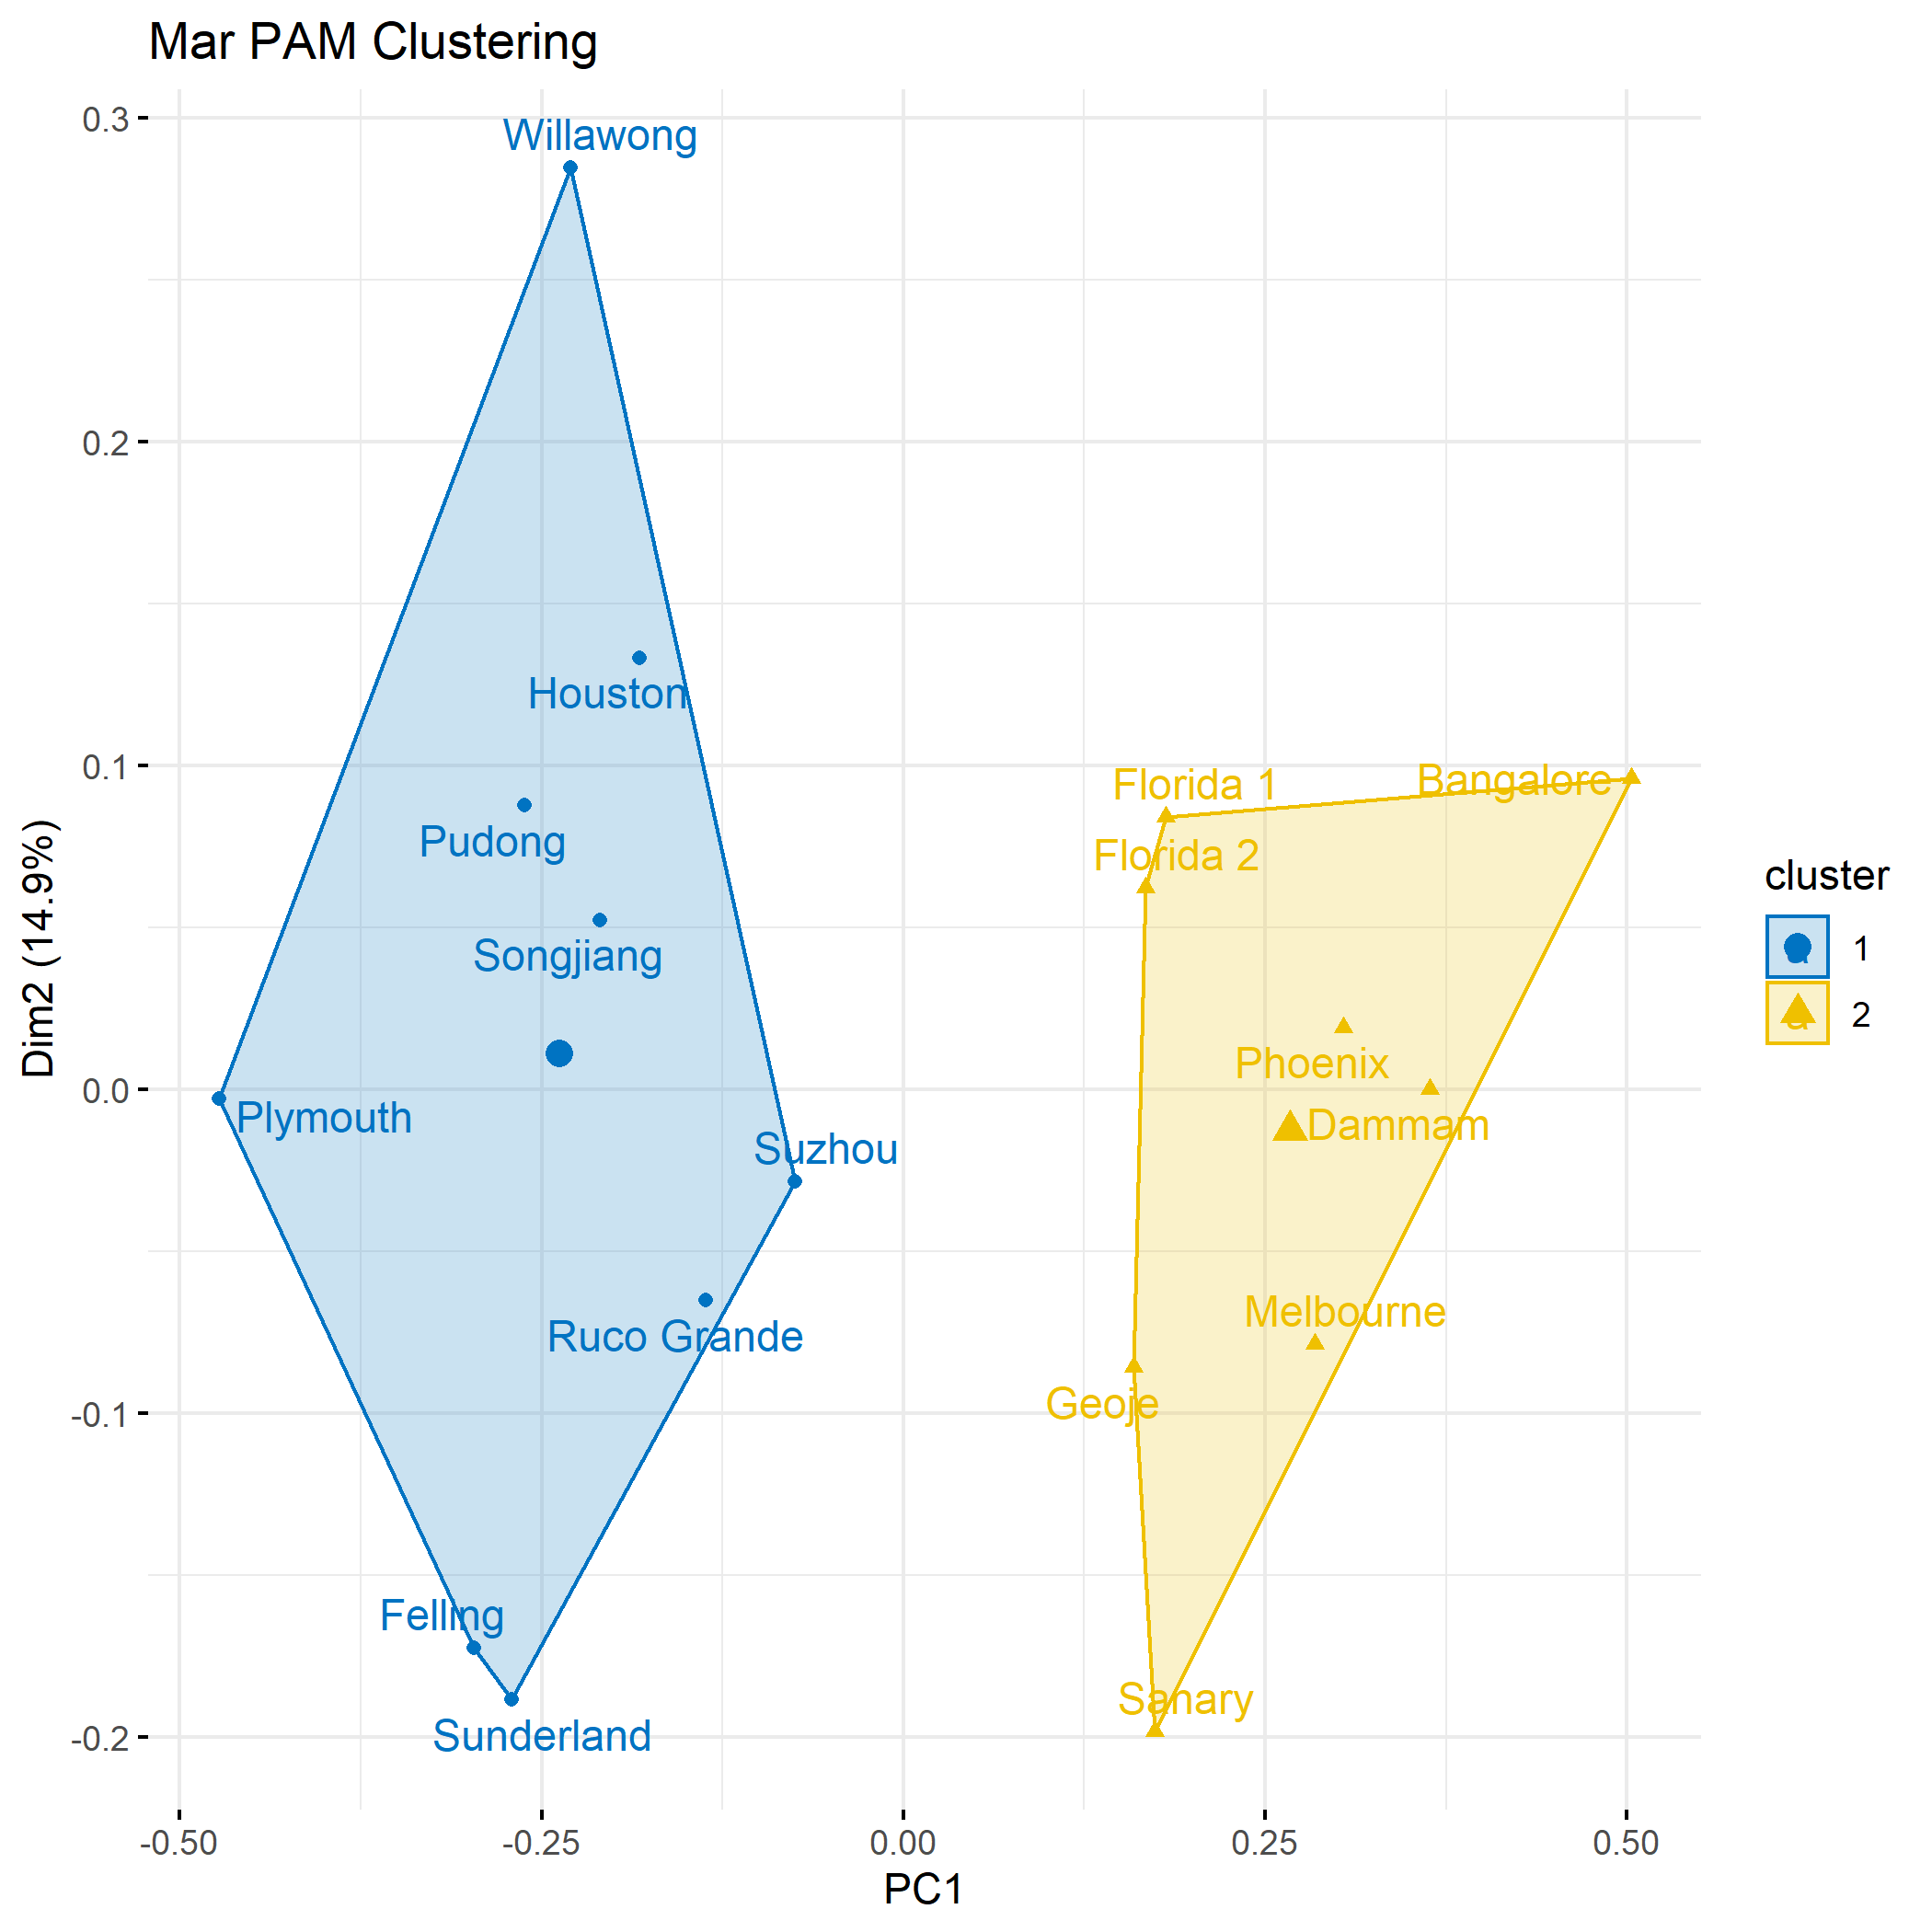
\includegraphics[width=.48\textwidth,height=6.5cm]{Mar_cluster.png}}\hfill
\subfloat[April PAM Clustering]{\label{sfig:d}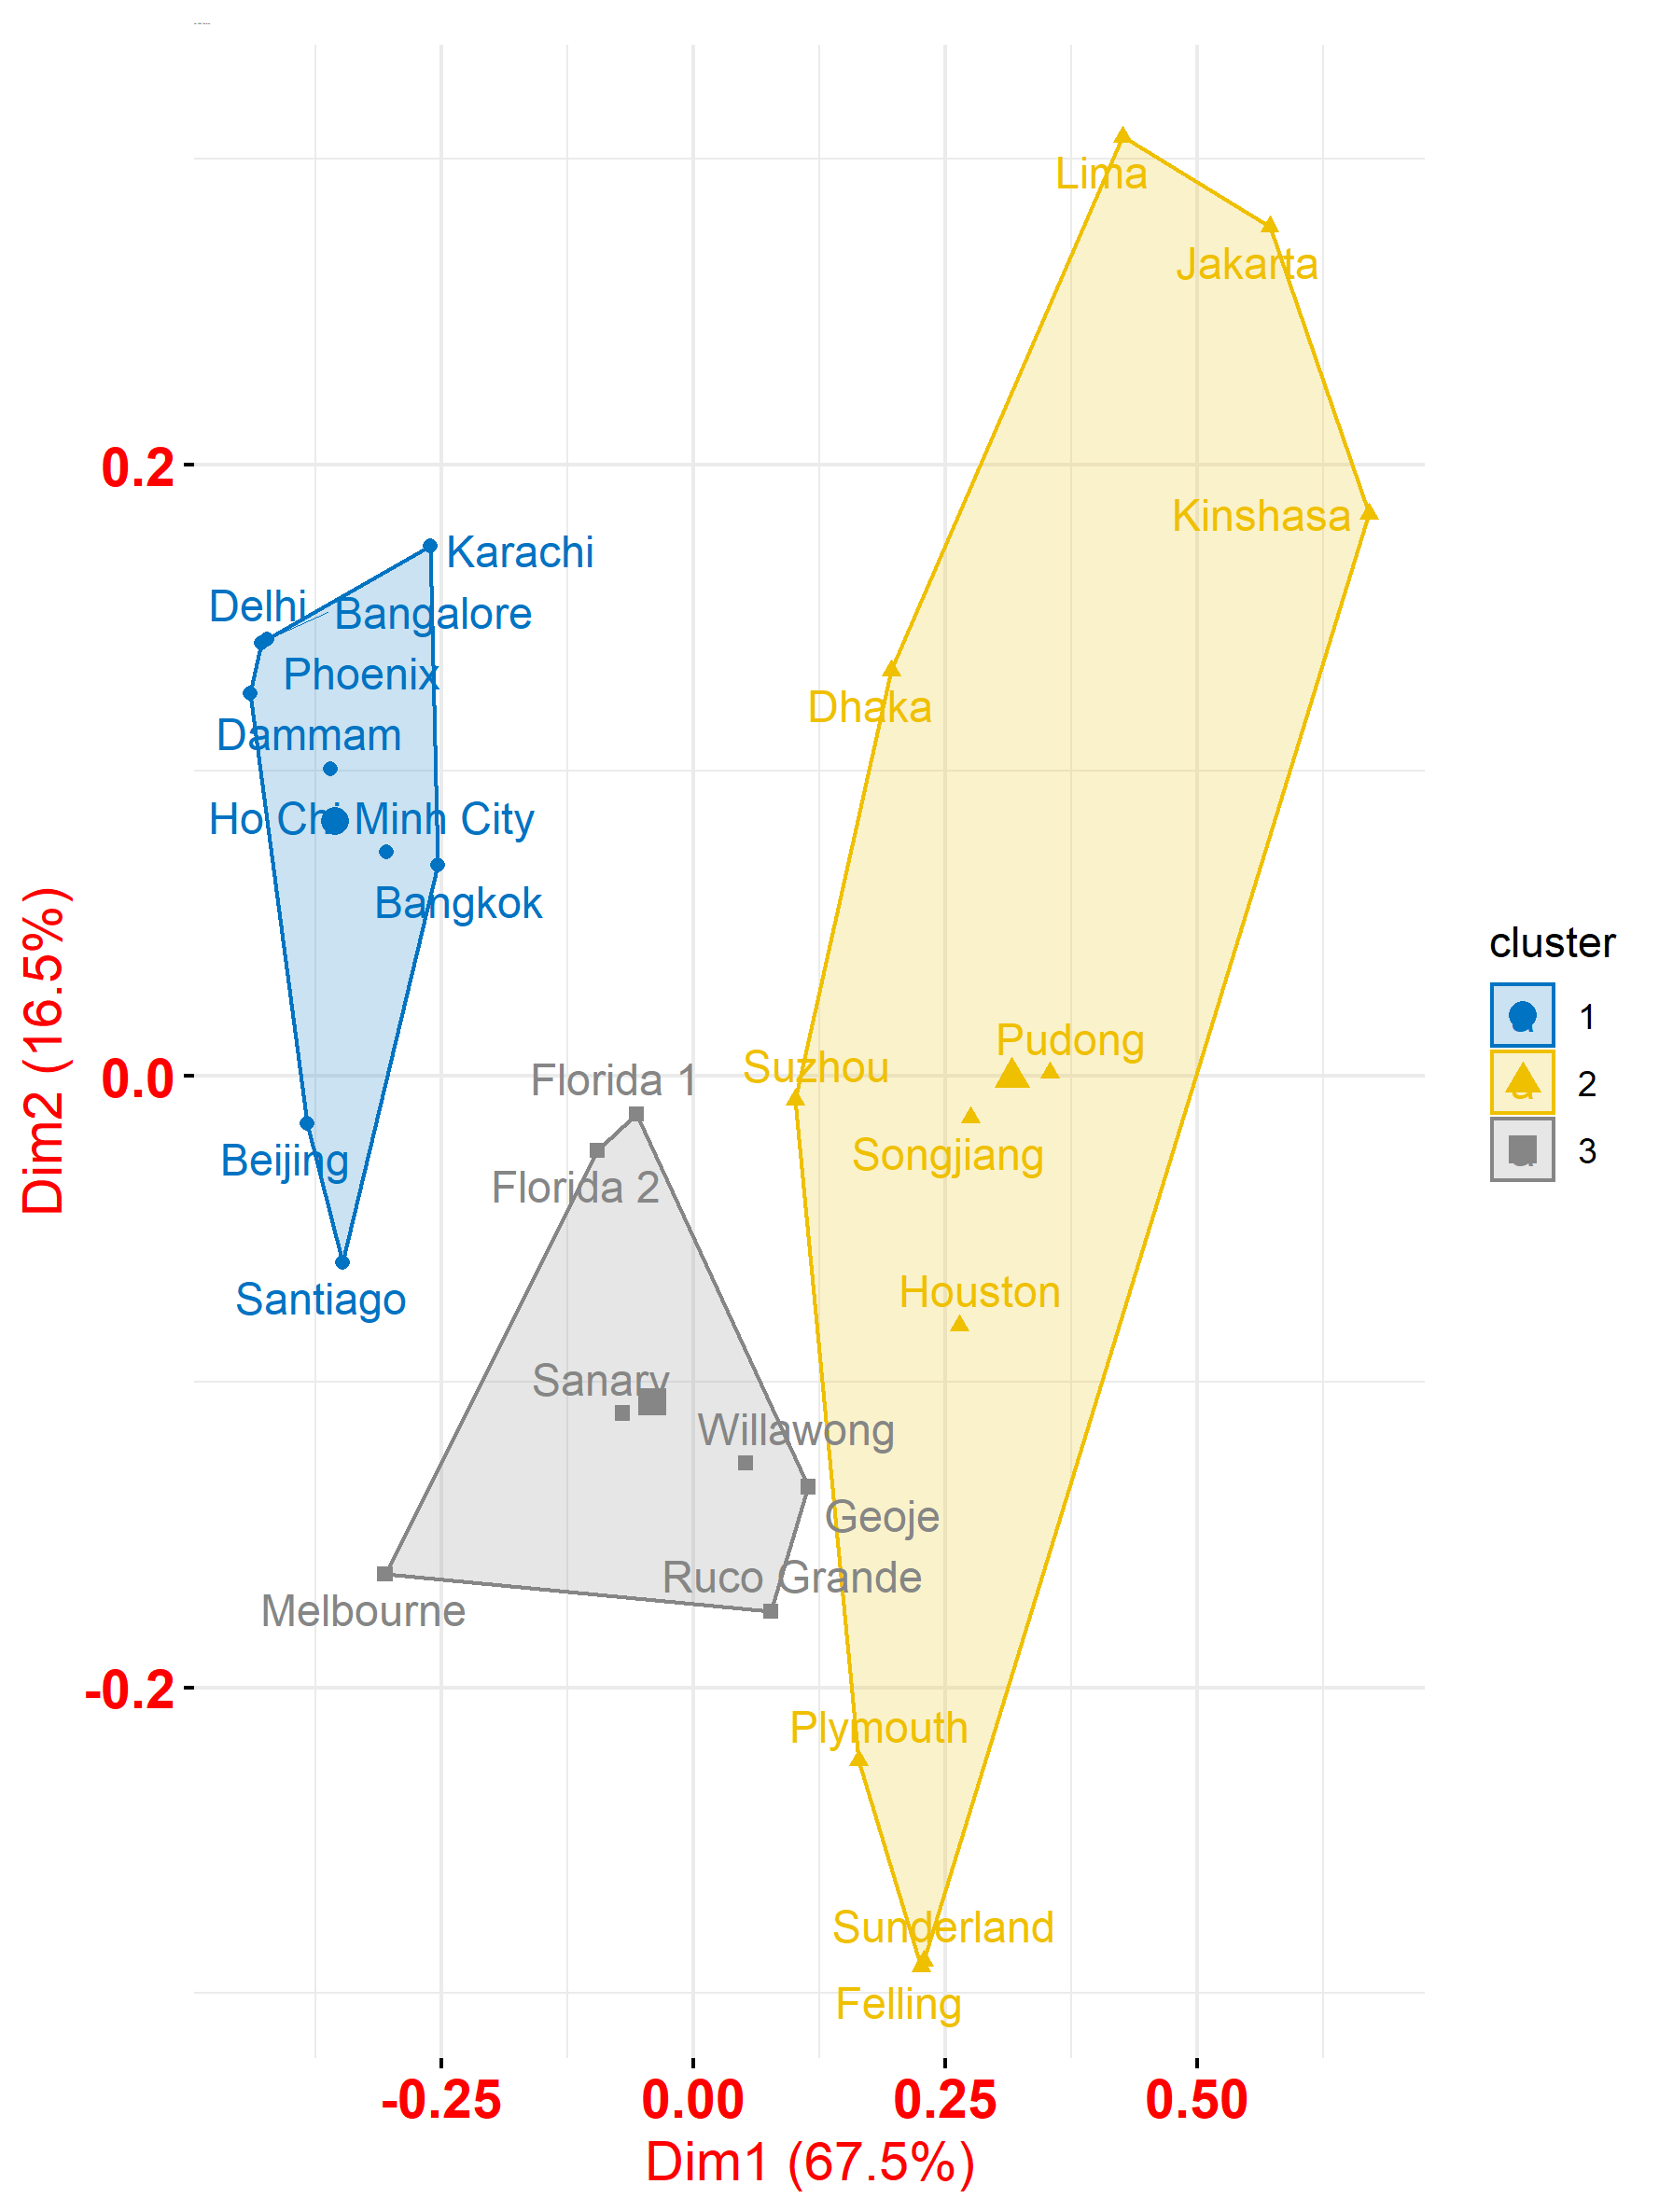
\includegraphics[width=.48\textwidth,height=6.5cm]{Apr_cluster.png}}\\
\subfloat[May PAM Clustering]{\label{sfig:e}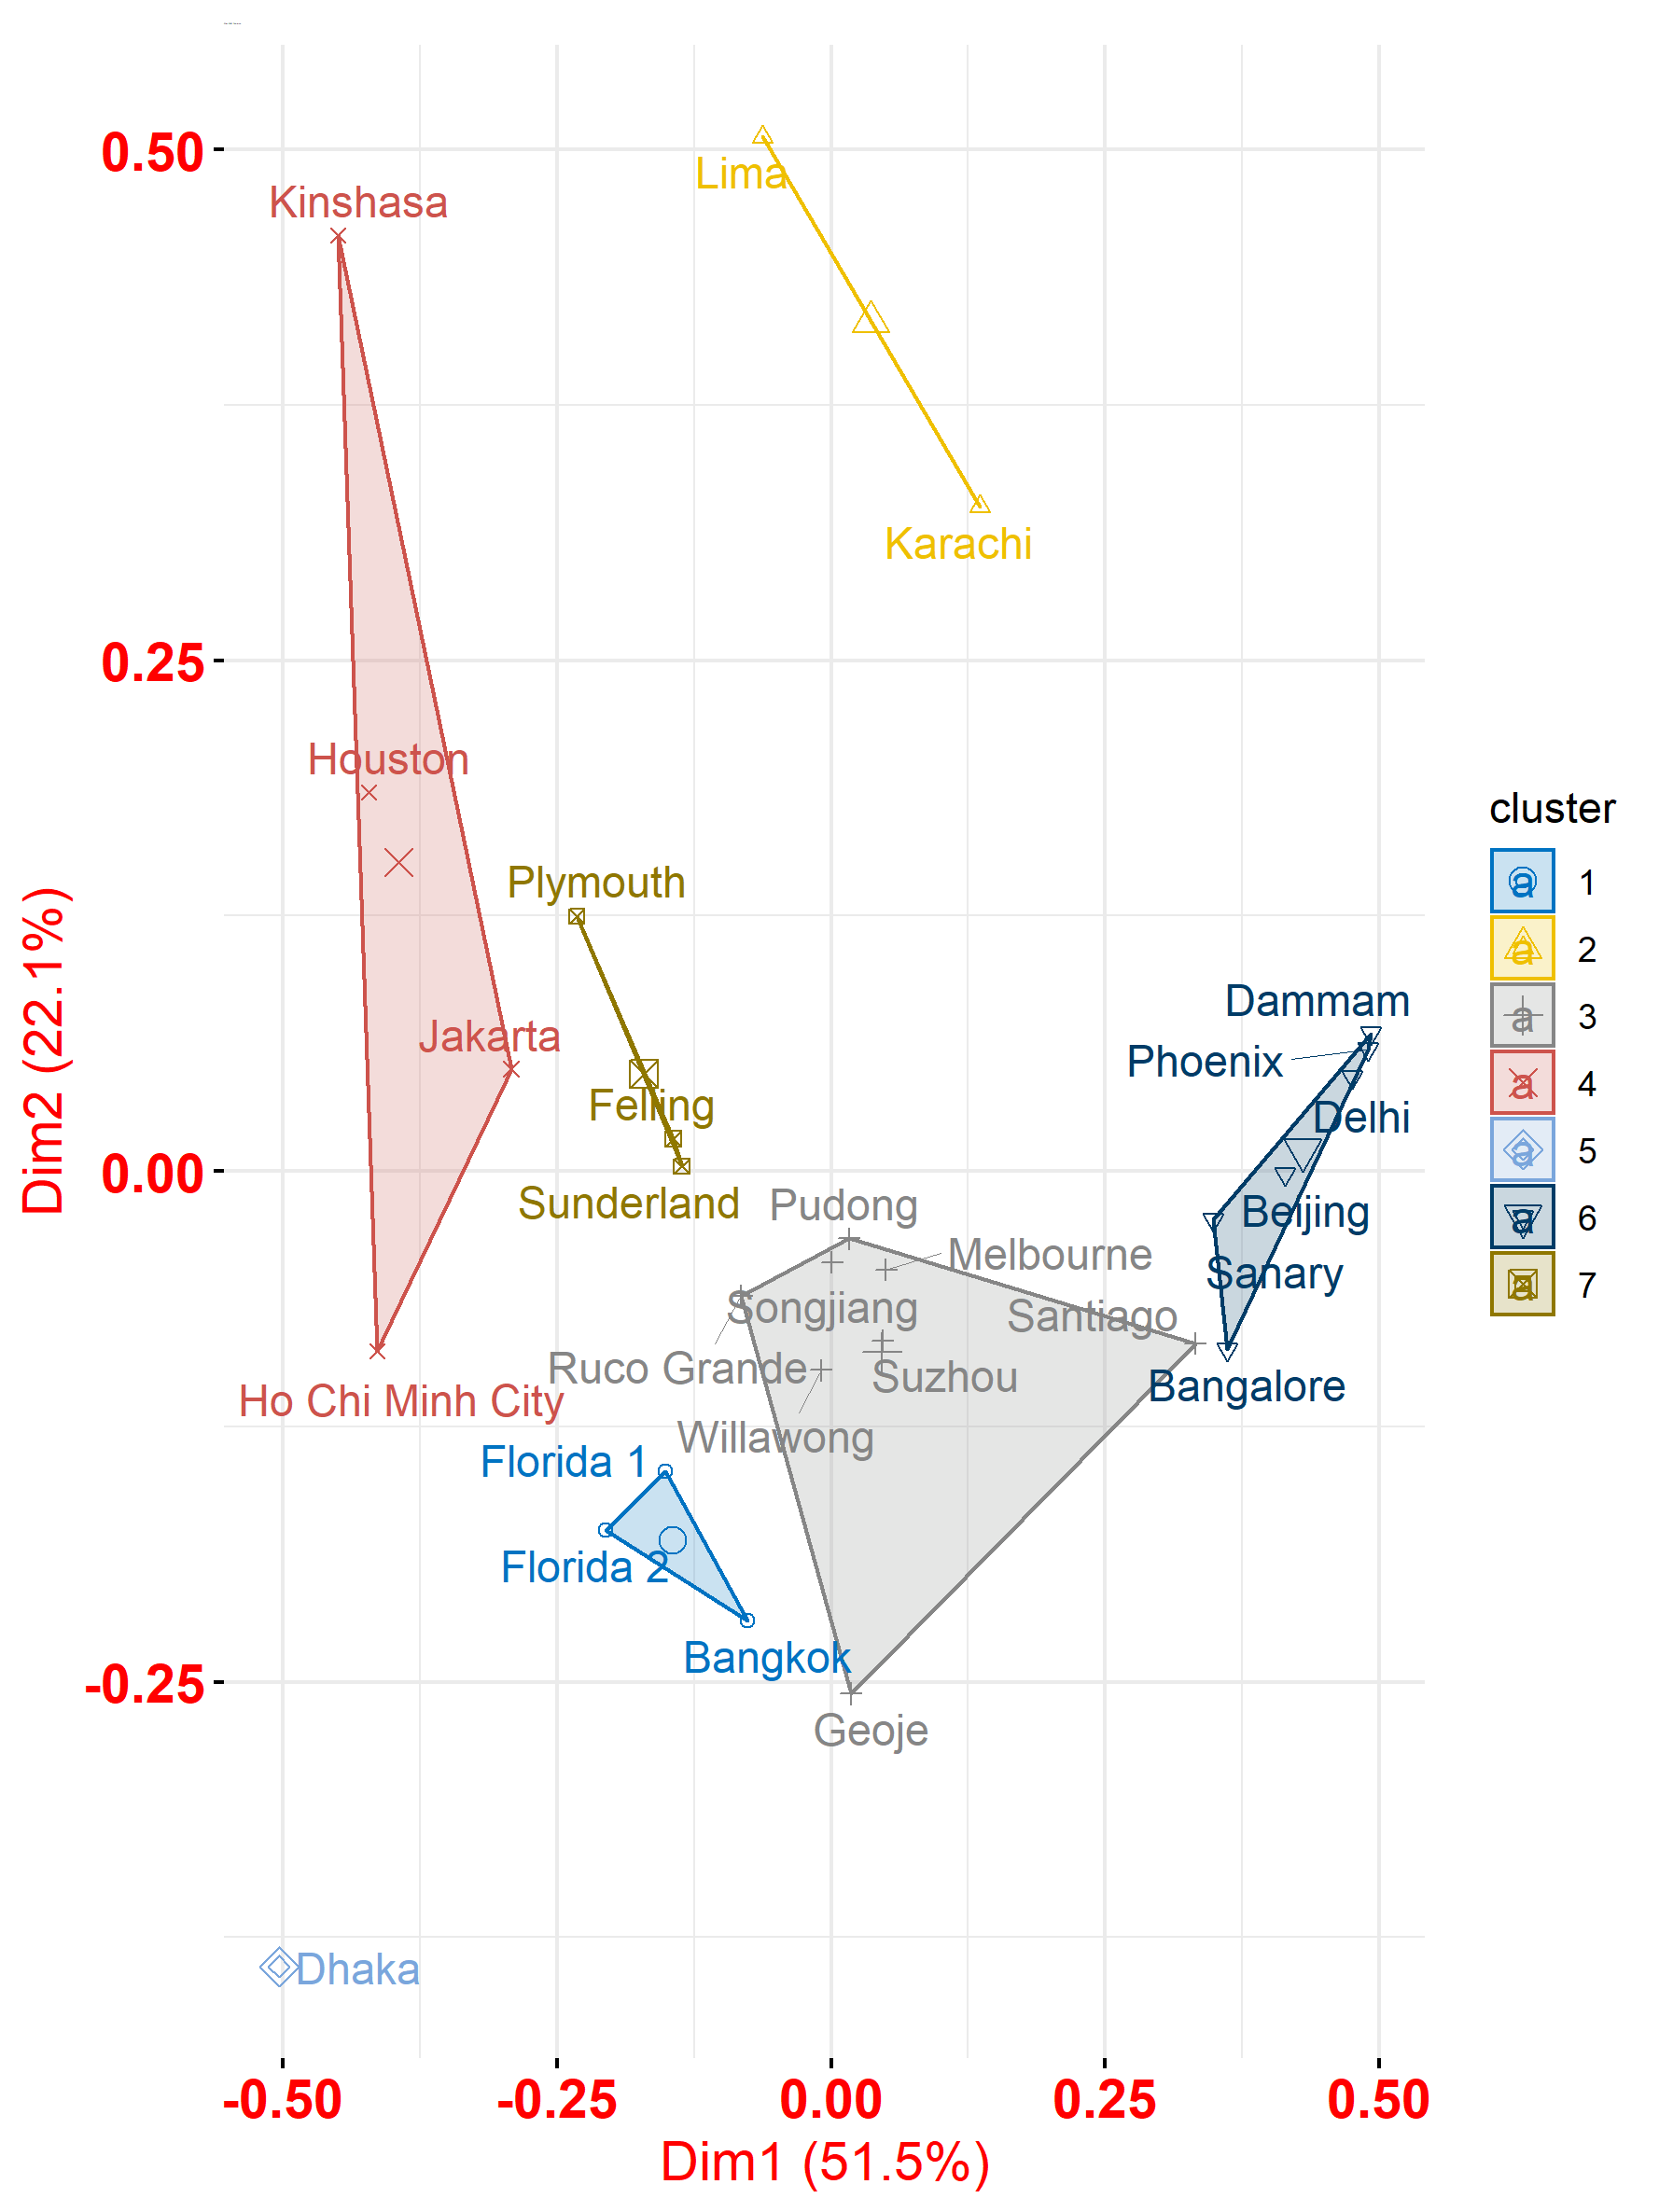
\includegraphics[width=.48\textwidth,height=6.5cm]{May_cluster.png}}\hfill
\subfloat[June PAM Clustering]{\label{sfig:f}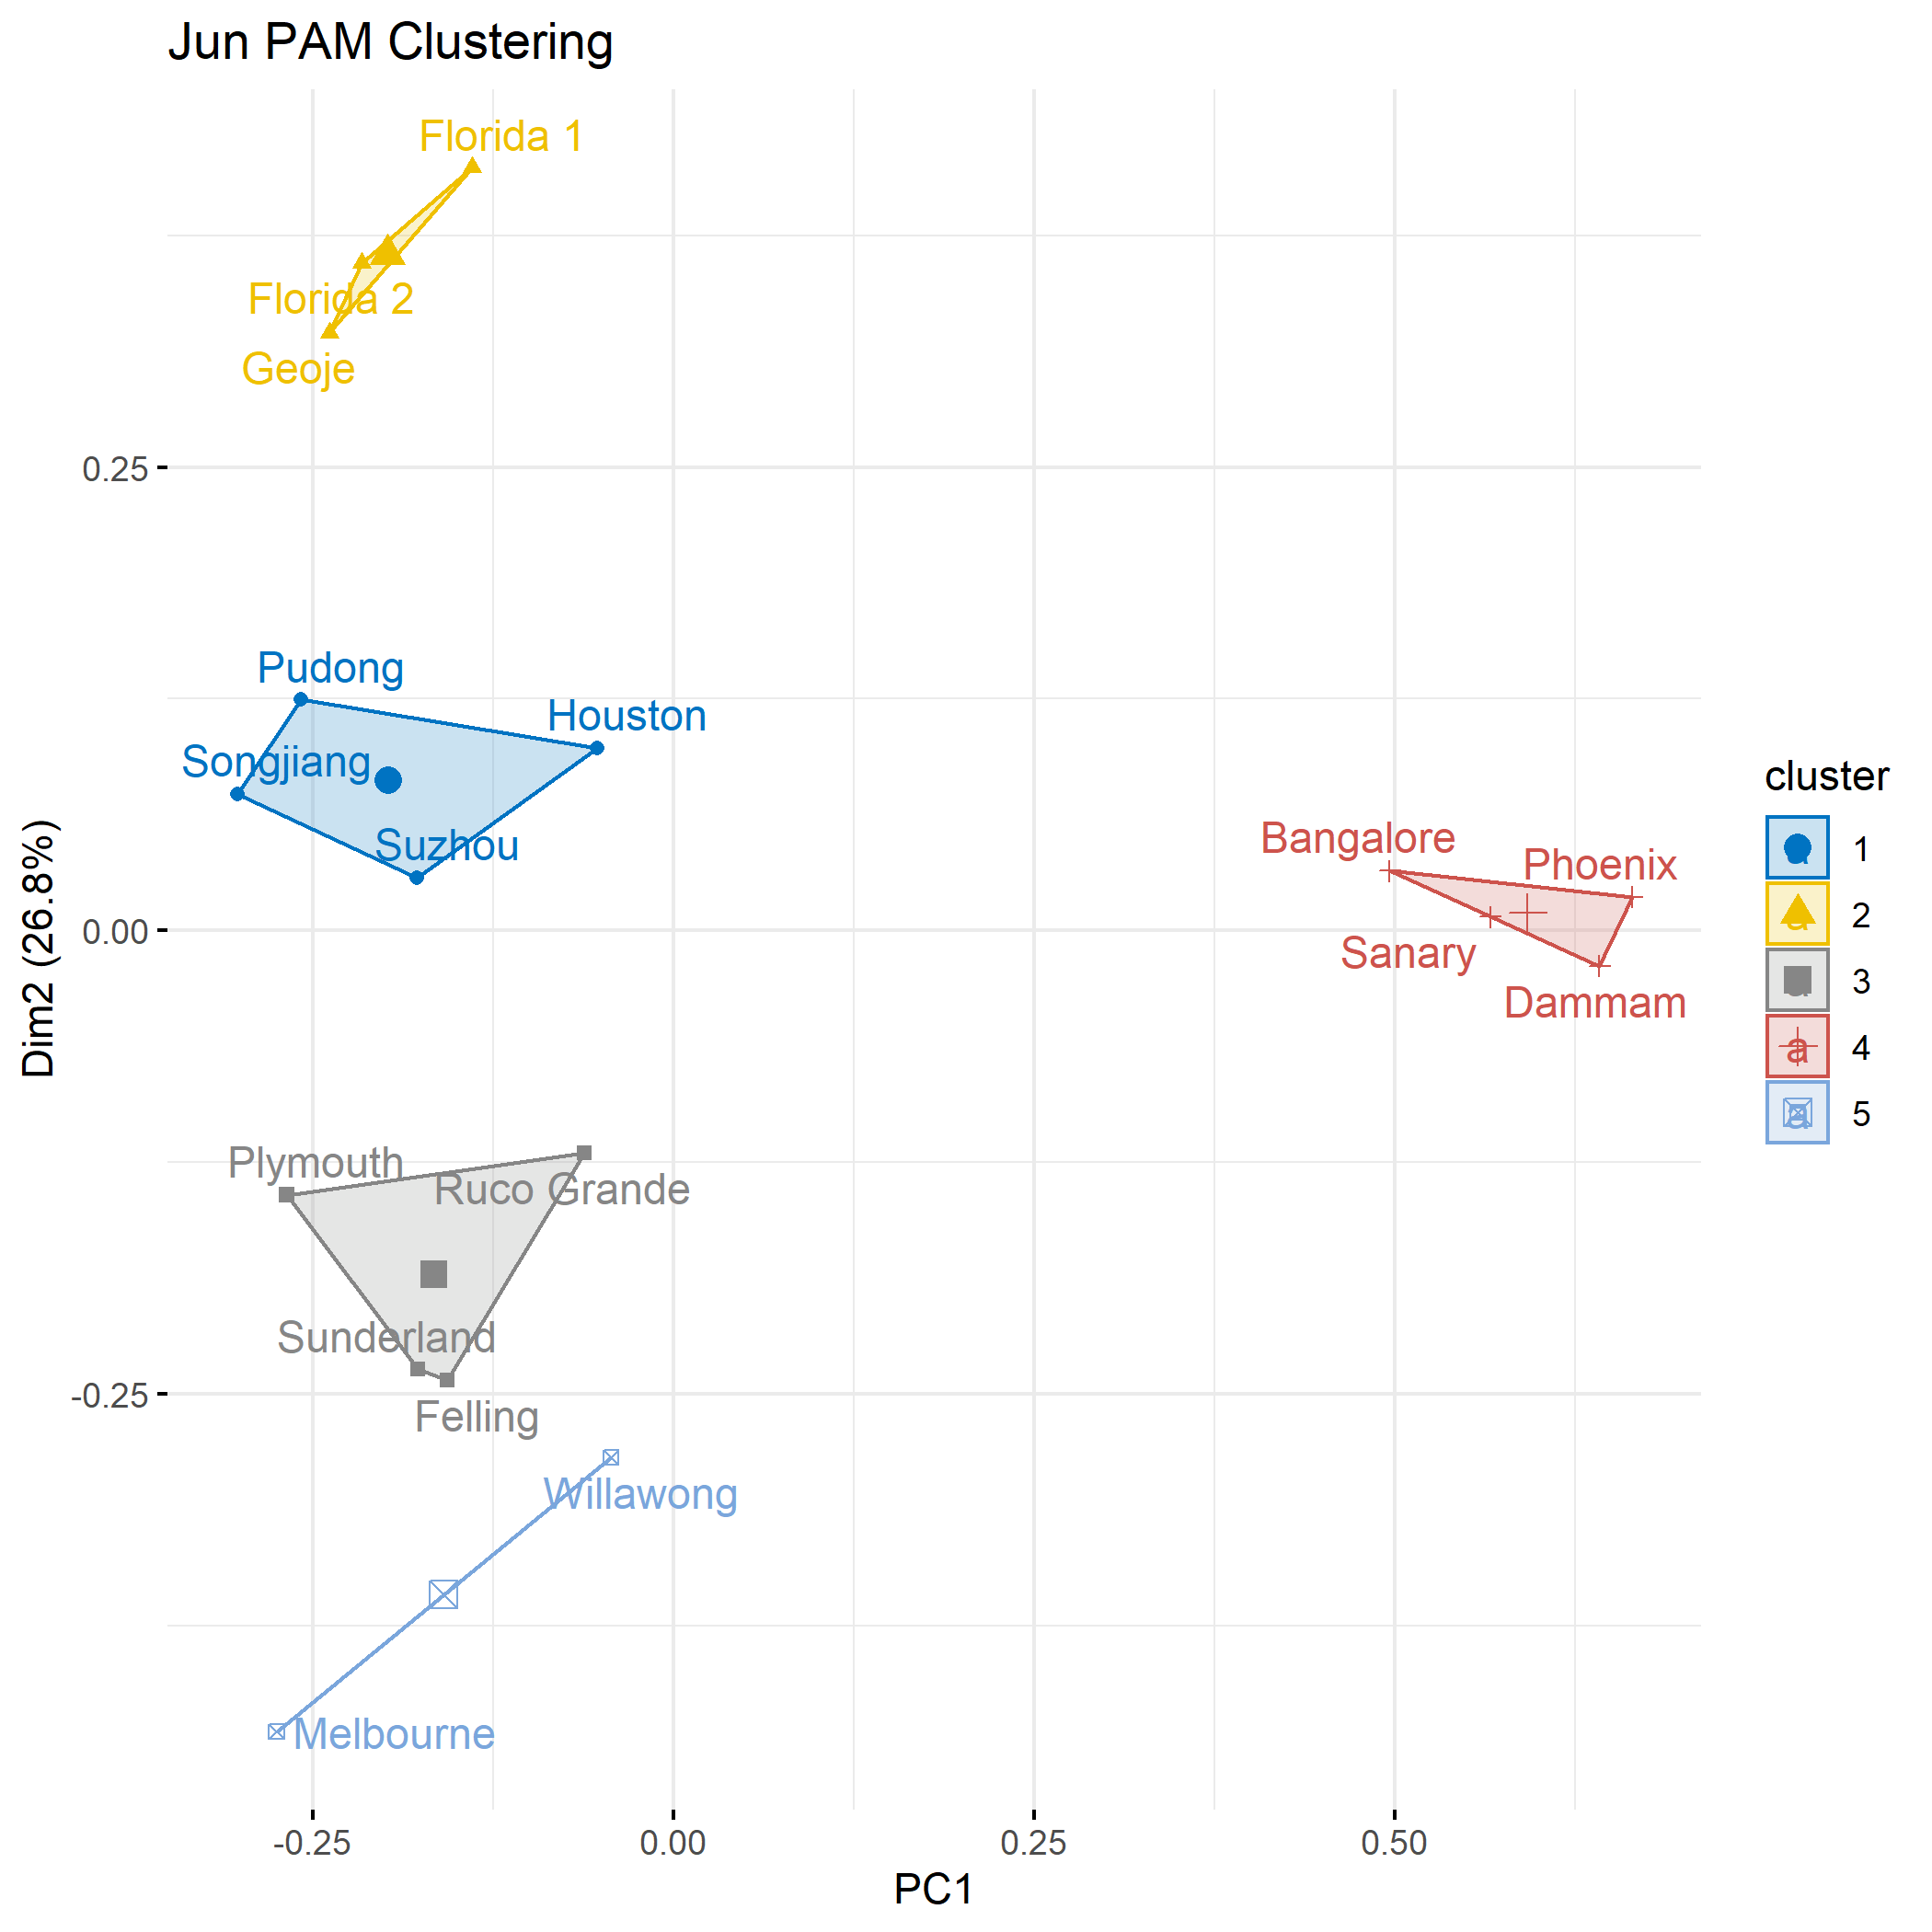
\includegraphics[width=.48\textwidth,height=6.5cm]{Jun_cluster.png}}\\
\caption{PAM Clustering of existing ETS for January-June}
\label{fig:jan_jun_ffp}
\end{figure}

\begin{figure}[h]
\centering
\subfloat[July PAM Clustering]{\label{sfig:g}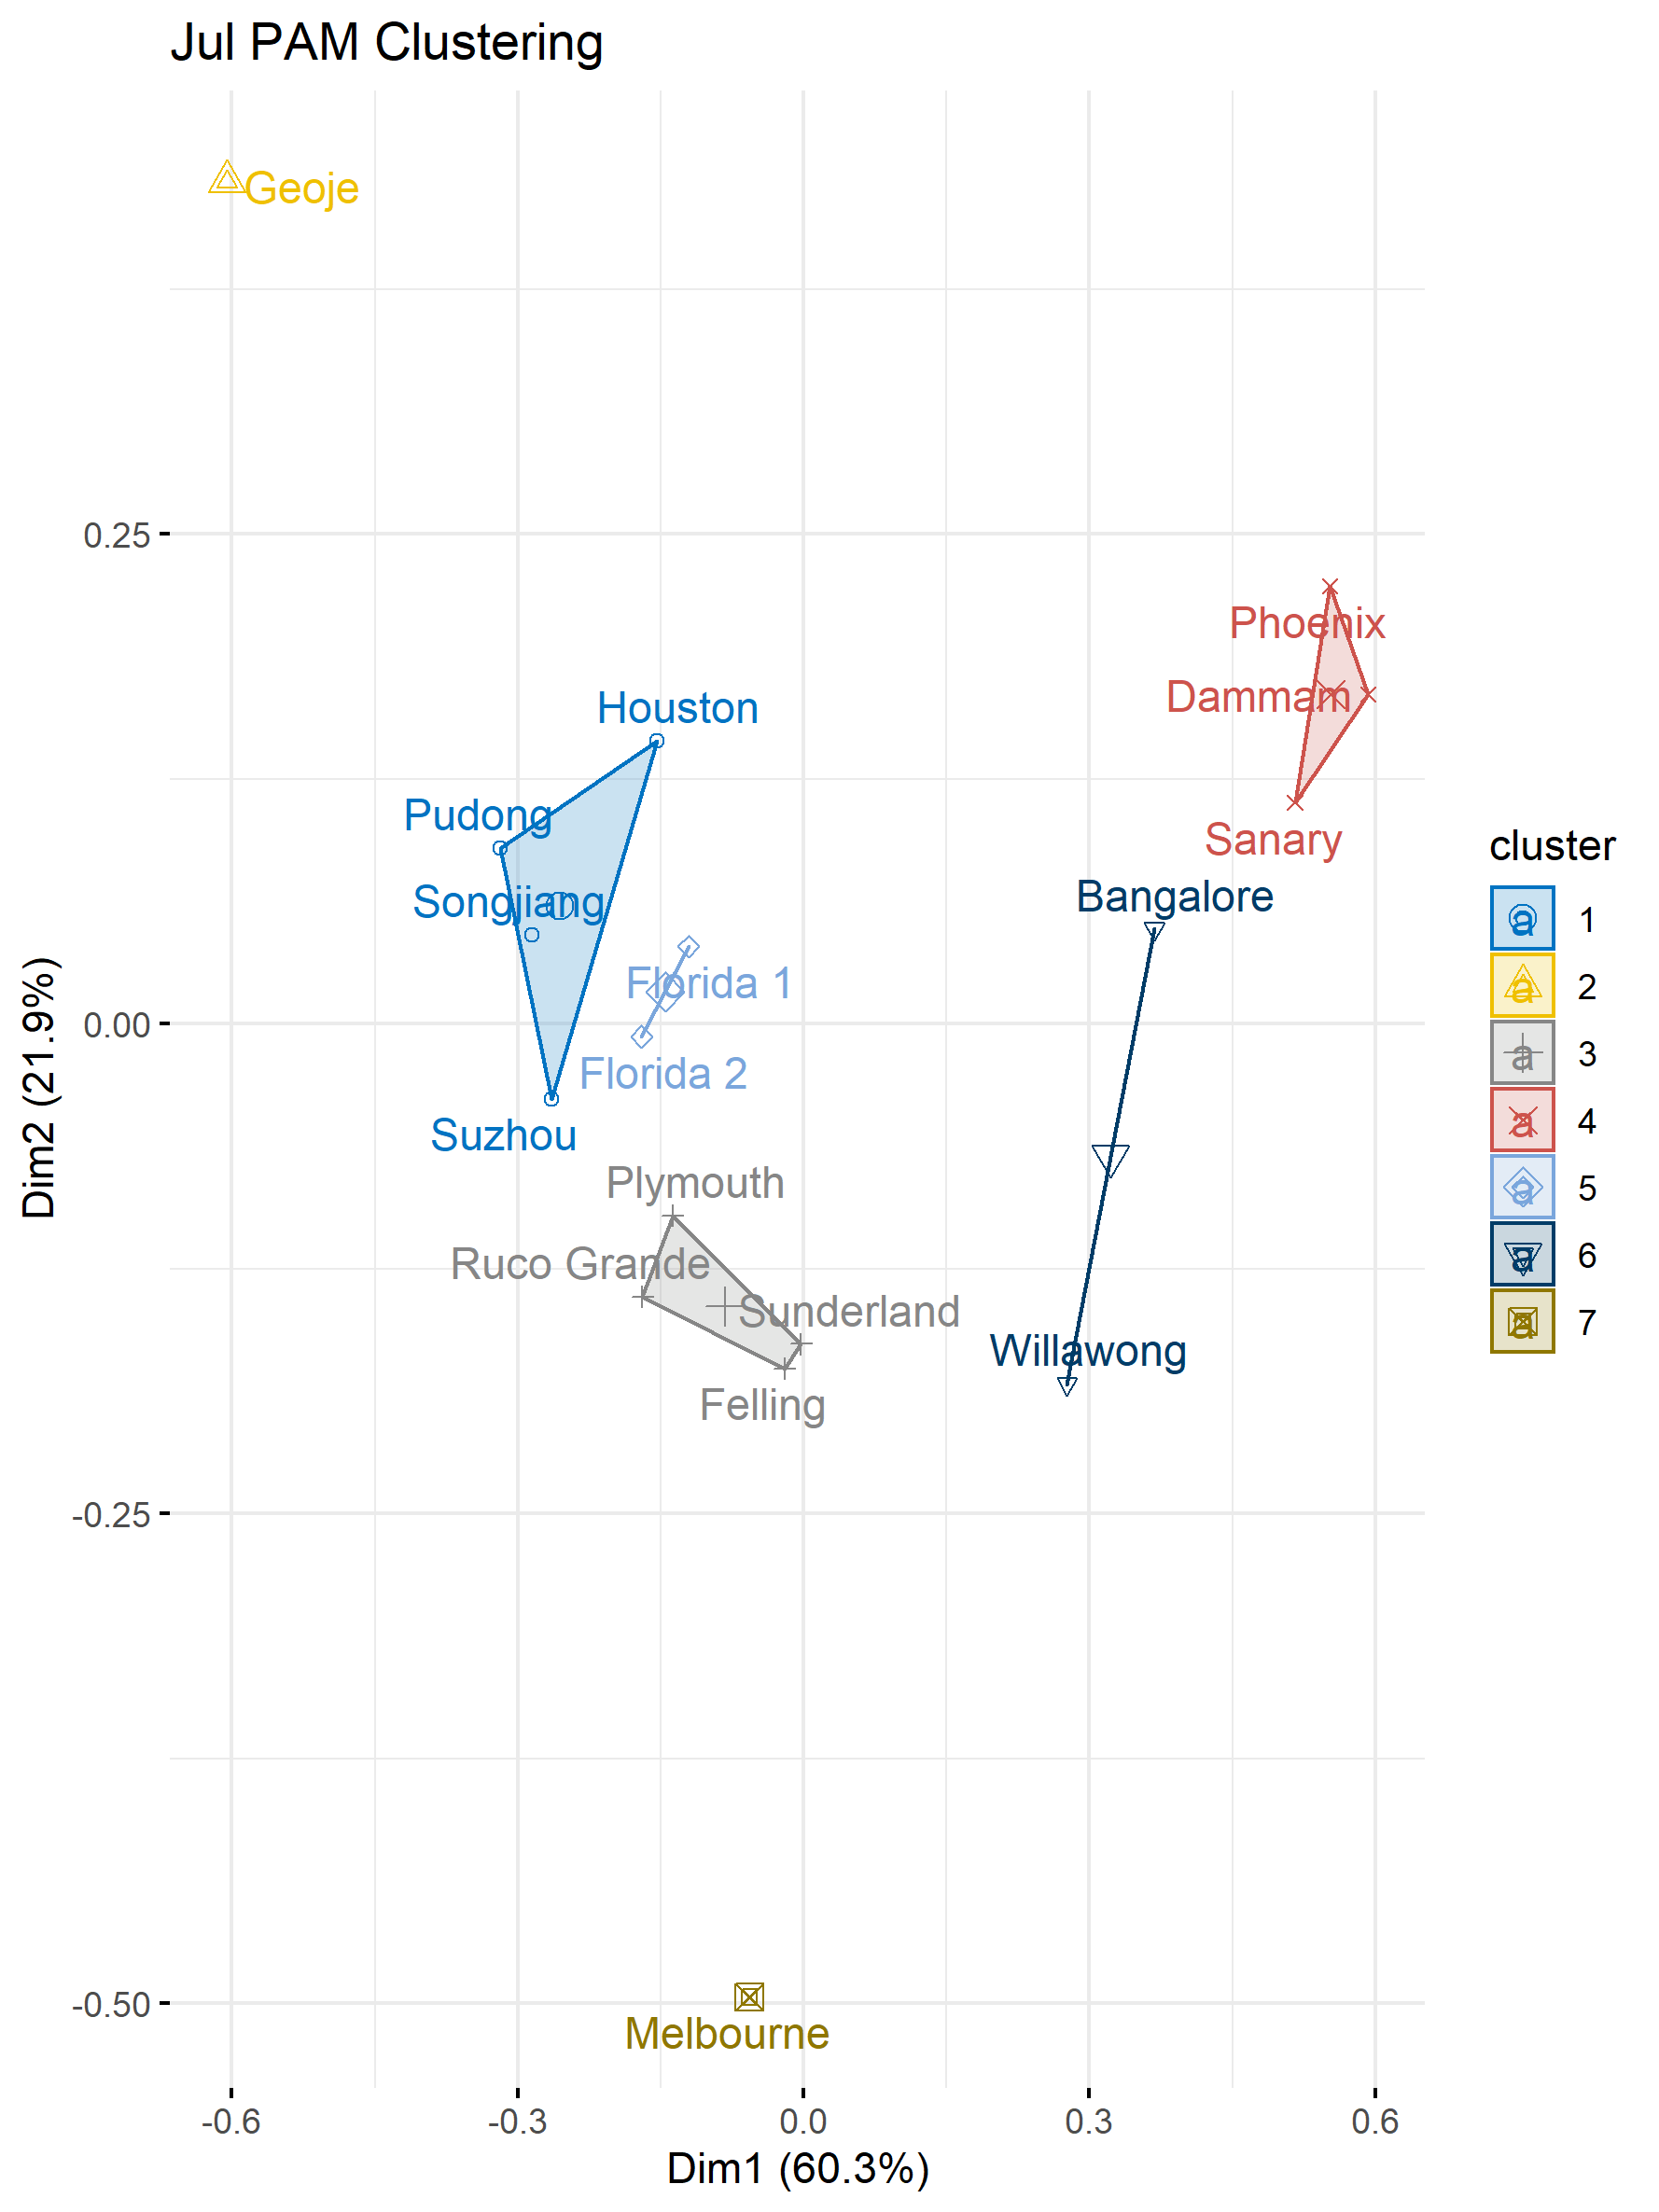
\includegraphics[width=.48\textwidth,height=6.5cm]{Jul_cluster.png}}\hfill
\subfloat[August PAM Clustering]{\label{sfig:h}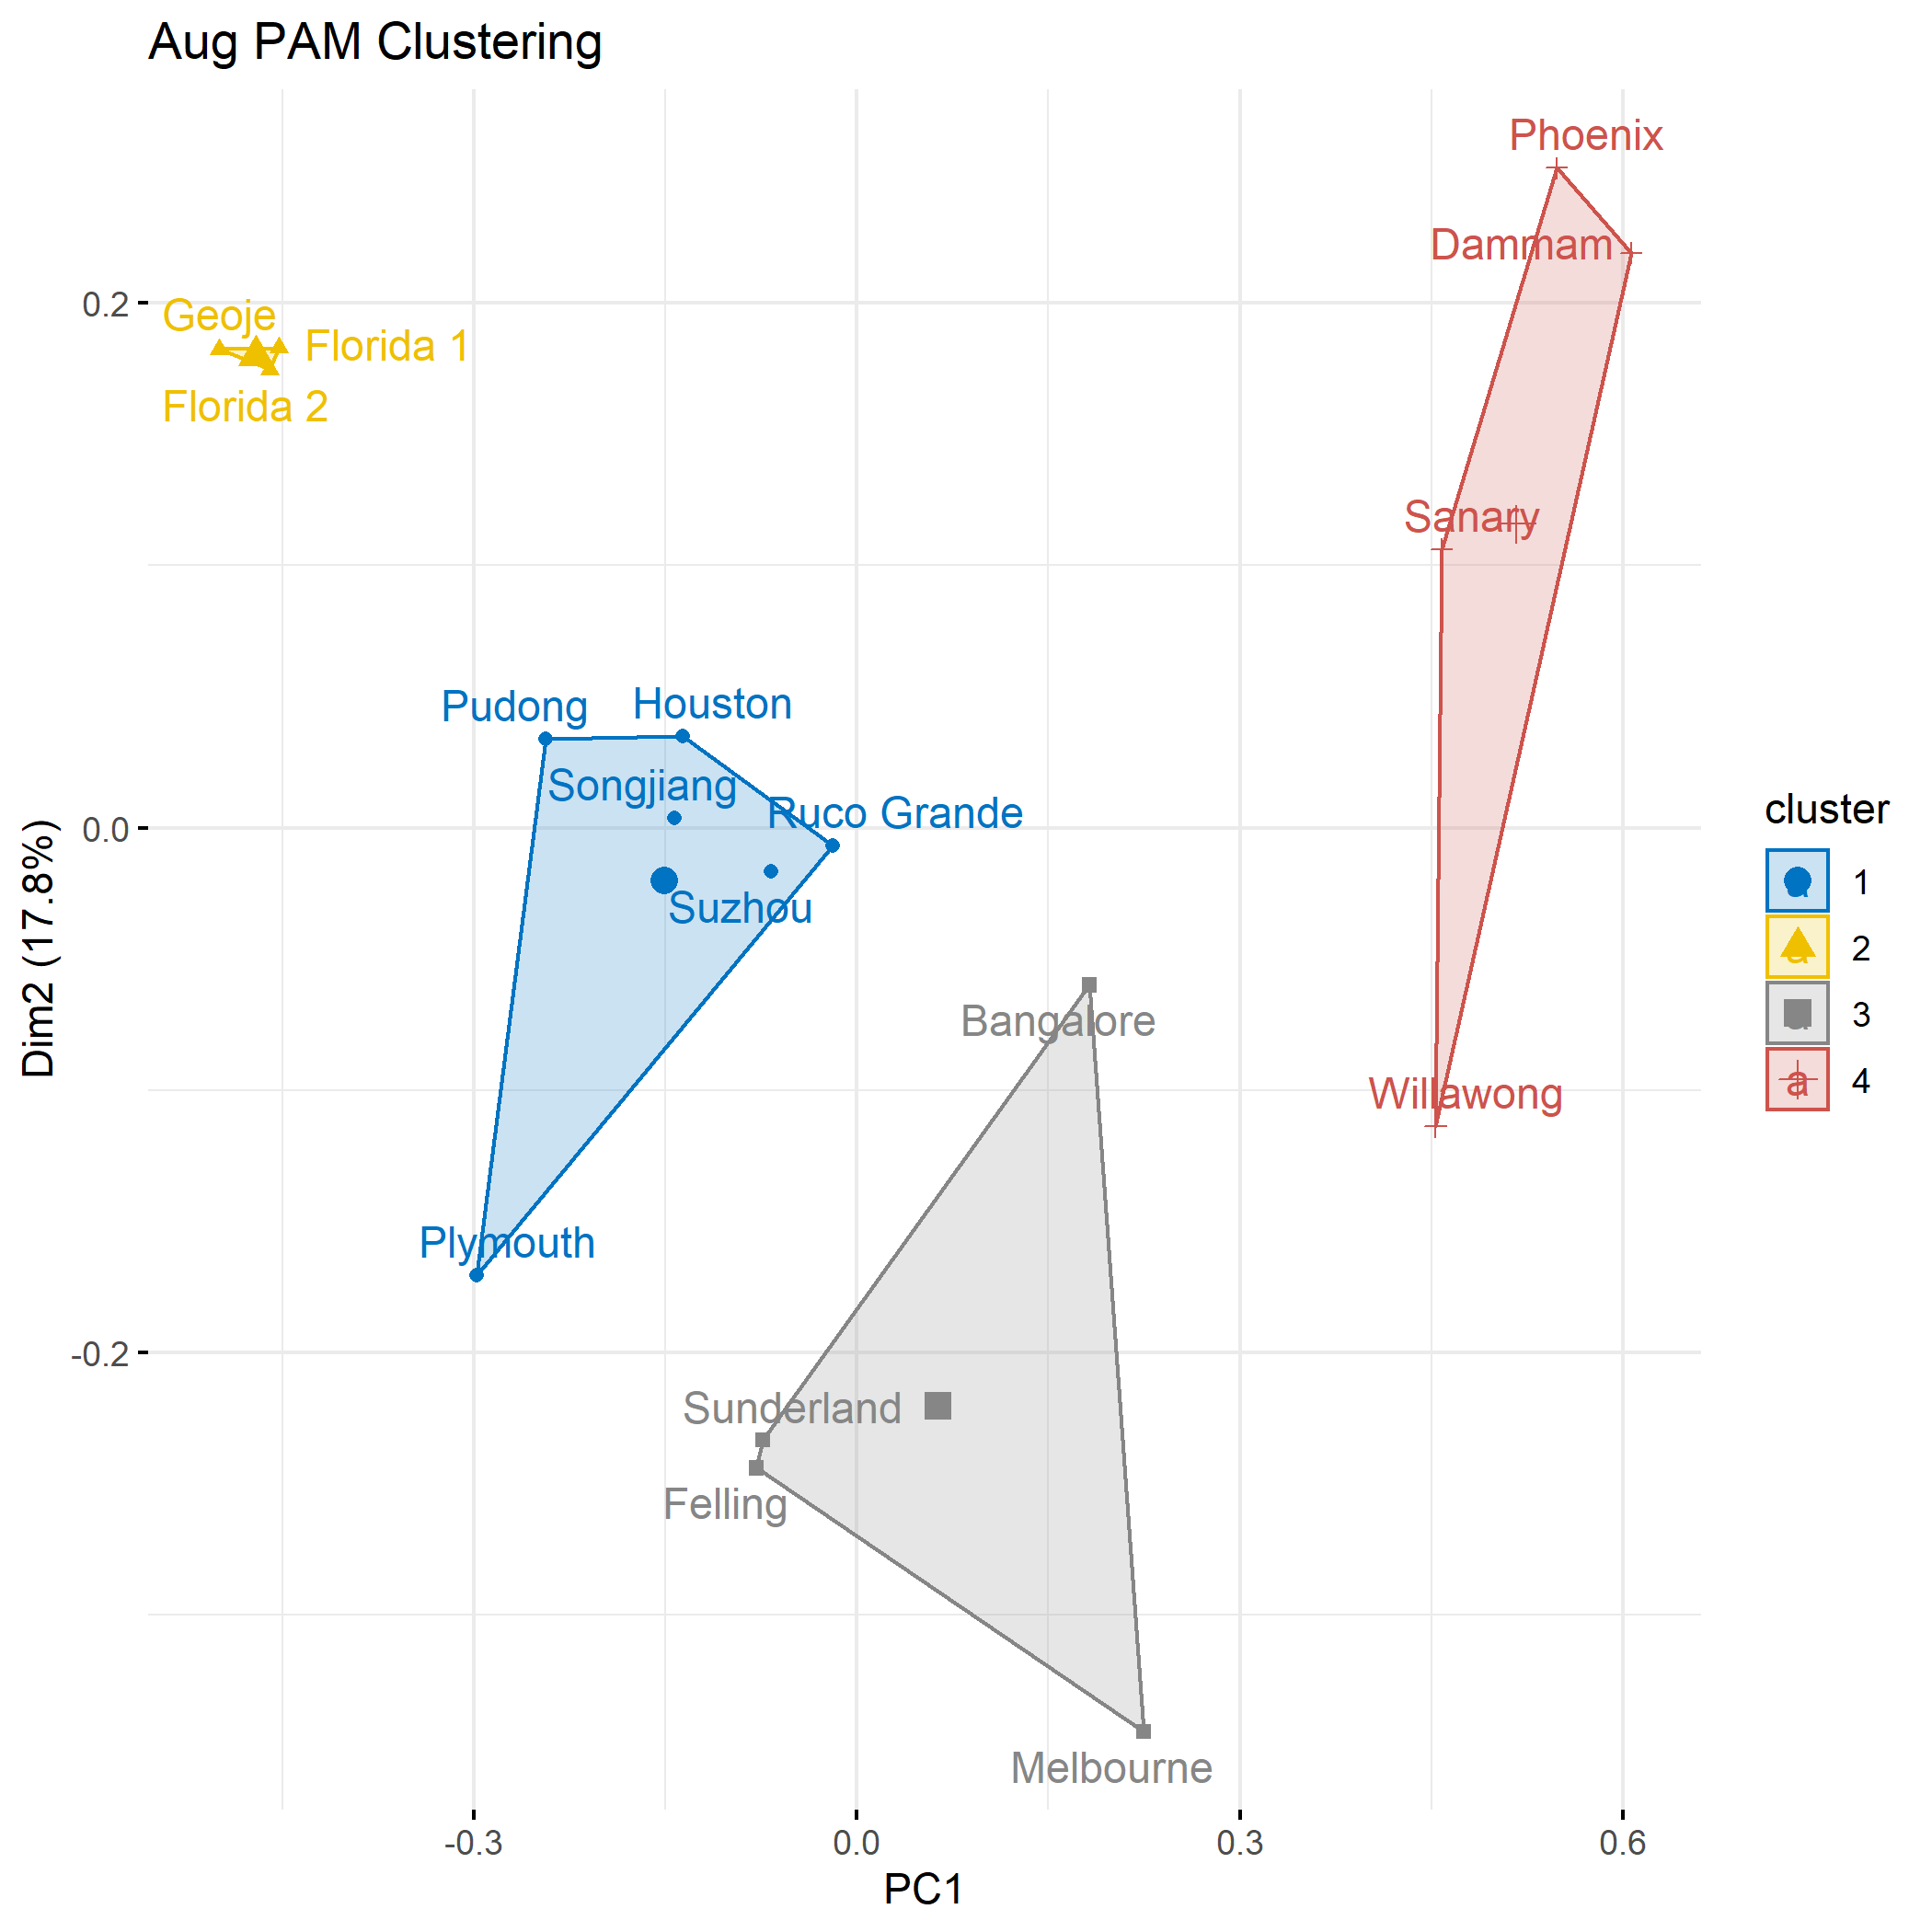
\includegraphics[width=.48\textwidth,height=6.5cm]{Aug_cluster.png}}\\
\subfloat[September PAM Clustering]{\label{sfig:i}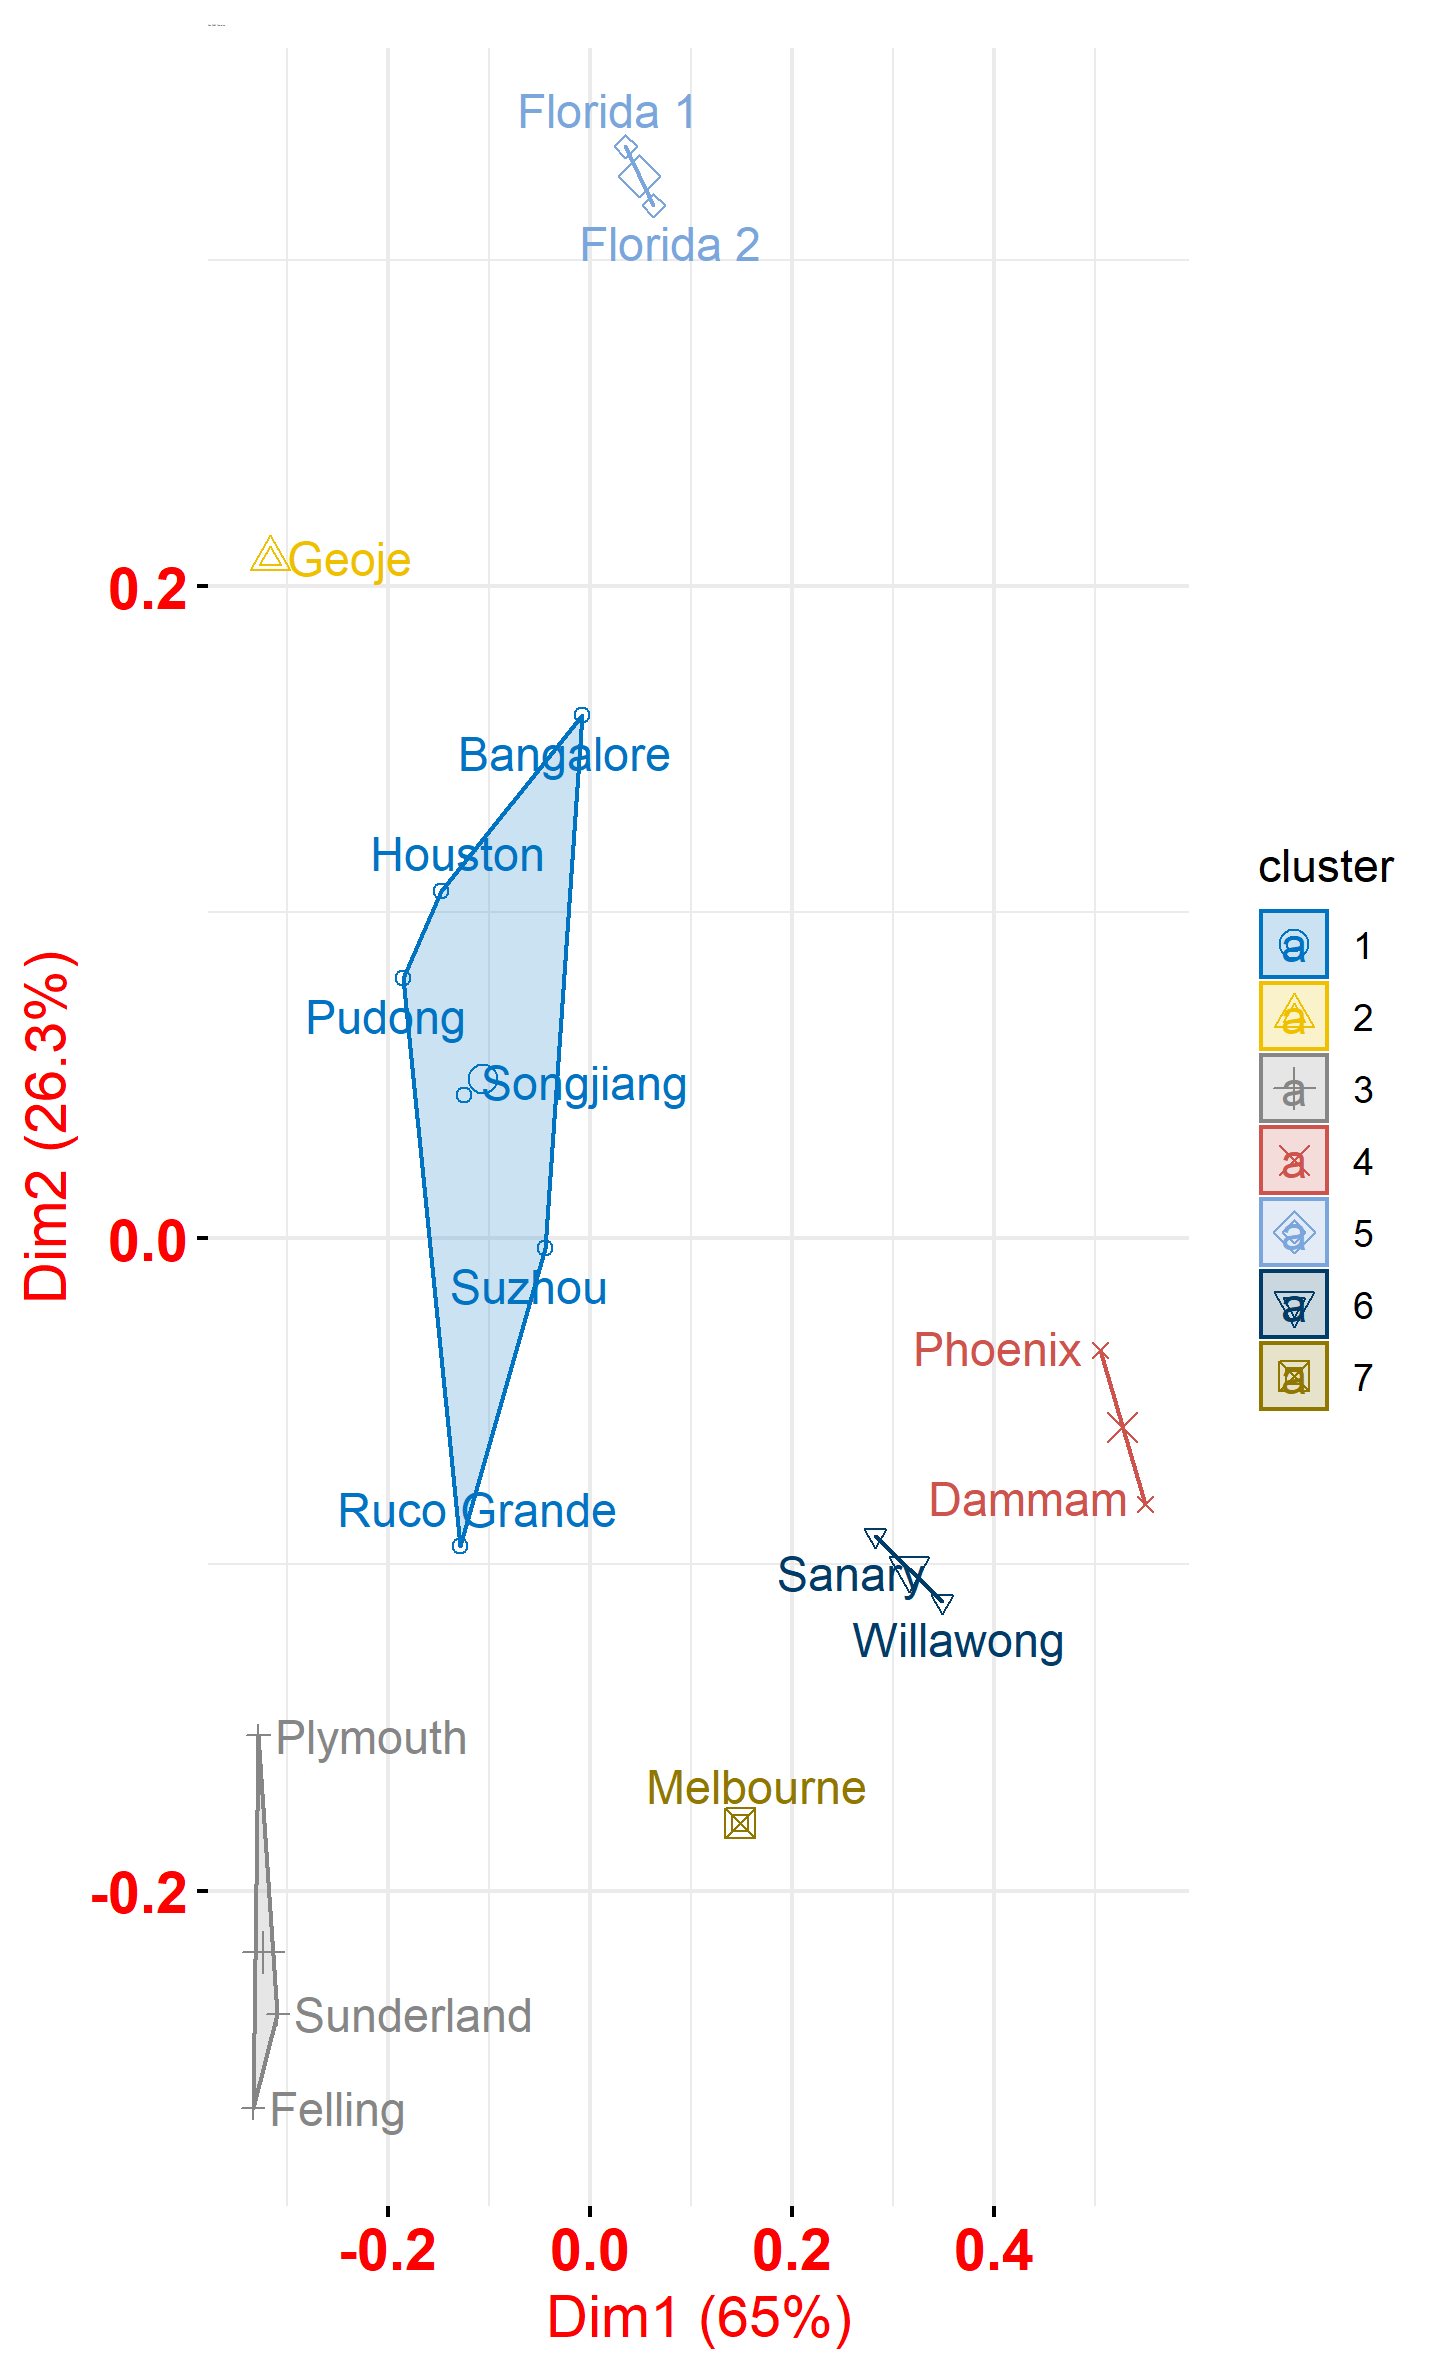
\includegraphics[width=.48\textwidth,height=6.5cm]{Sep_cluster.png}}\hfill
\subfloat[October PAM Clustering]{\label{sfig:j}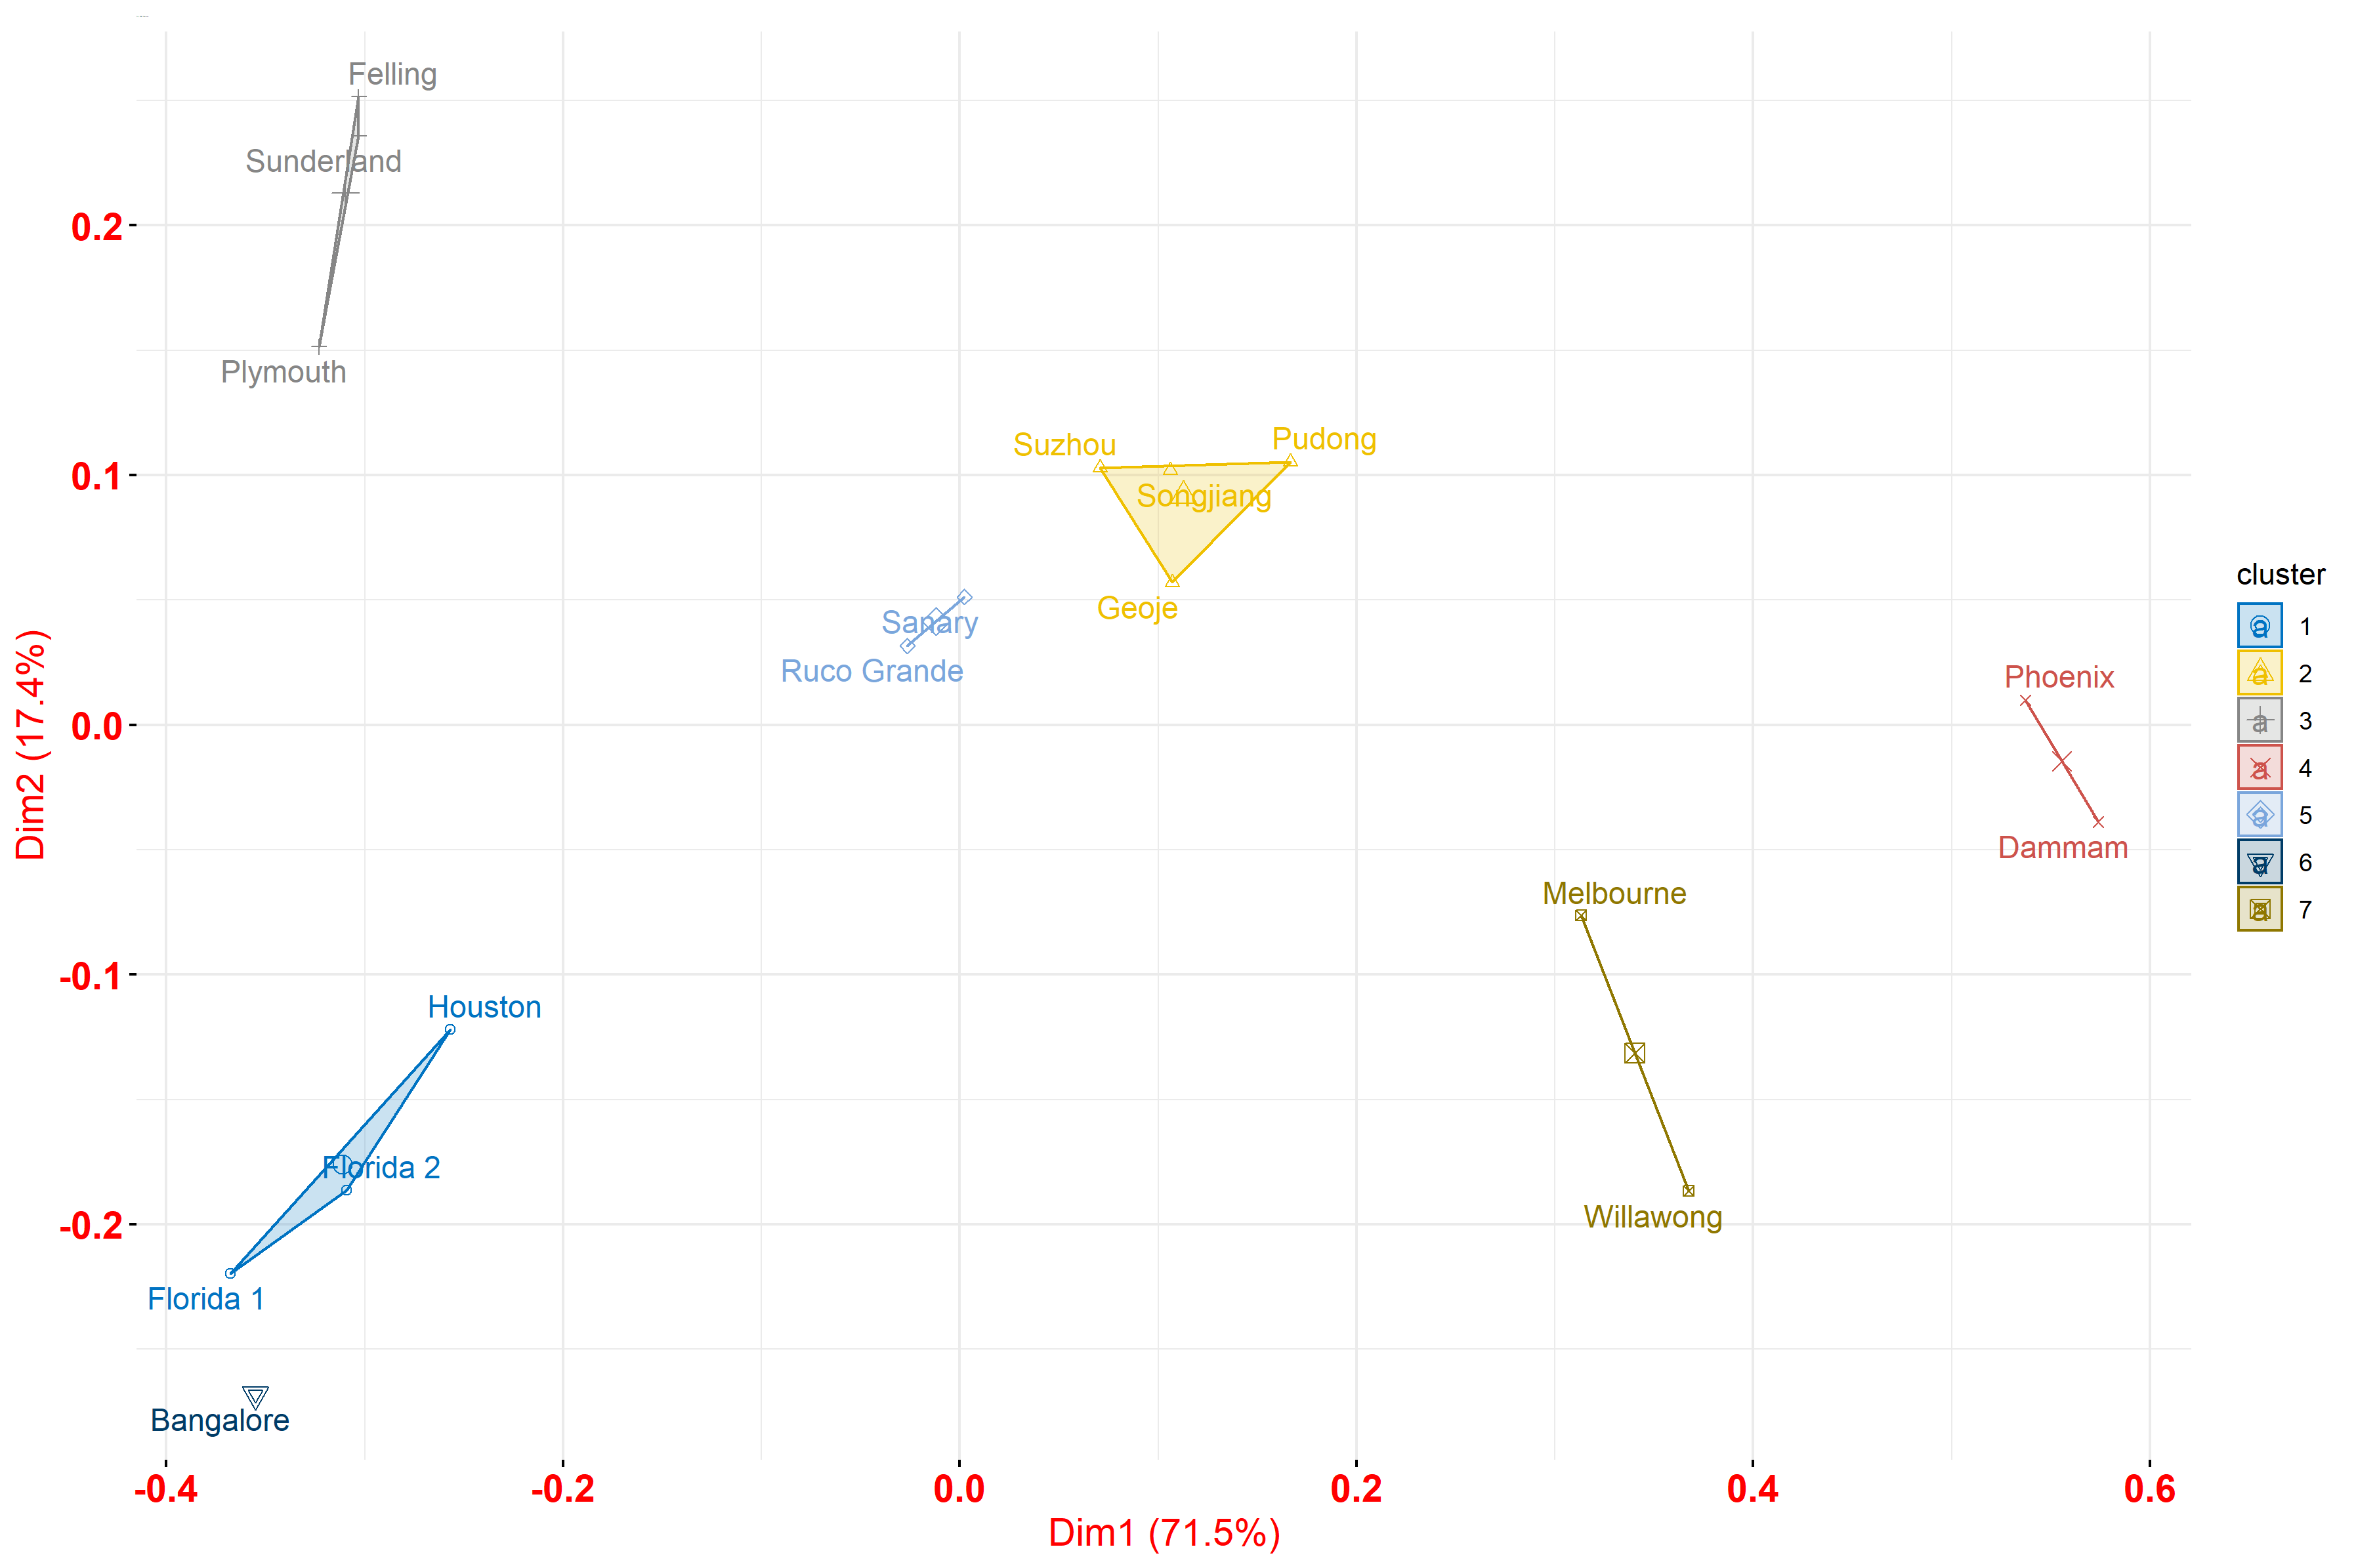
\includegraphics[width=.48\textwidth,height=6.5cm]{Oct_cluster.png}}\\
\subfloat[November PAM Clustering]{\label{sfig:j}\includegraphics[width=.48\textwidth,height=6.5cm]{Nov_cluster.png}}\hfill
\subfloat[December PAM Clustering]{\label{sfig:j}\includegraphics[width=.48\textwidth,height=6.5cm]{Dec_cluster.png}}\\
\caption{PAM Clustering of existing ETS for July-December}
\label{fig:jul_dec_ffp}
\end{figure}

\subsection{Comparison of Exposure Testing sites to Global Environments}
Figure \ref{fig:dtw_maps} shows the raster map relating to each ETS comparison with the globe. These rasters clearly show a heatmap of high similarity and low similarity. The more blue an area of the globe is the less similar that location is to the given ETS. It is clear from these maps that some ETS have more widespread similarity whereas others are more unique. Particularly unique are Melbourne... this is in agreement with the analysis discussed in section \ref{hcpc} and gives more confidence in these results. 

Figure \ref{fig:dtw_max} is a heatmap showing the maximum values for each cell in the raster when compared to any of the exposure testing sites. This map is therefore an indication of how similar AkzoNobel's ETS are to all global environments. It is clear from this map that certain areas of the globe are not significantly similar to the environment of any of the ETS and it would therefore be beneficial to have additional ETS that reflect these environments. This would give more confidence in evaluation of product performance.  
\subsection{Recommendation of new Exposure Testing Sites}

In order to identify the best possible locations for additional ETS the maximum similarity map shown in figure \ref{fig:dtw_max} was combined with a data set containing the locations of many many major cities of the world and also provincial capitals. The world cities data set also contains estimations of population taken from the United Nations Census. Ten additional ETS locations have been suggested by selecting only cities from the world cities data set that were in the highest population rank category and sorting  them by maximum similarity value from smallest to largest. These ten locations are Bangkok, Lima, Santiago, Kinshasa, Jakarta, Ho Chi Minh City, Dhaka, Beijing, Deli and Karachi. 

The method outlined in section \ref{hcpc} has been used again with the addition of these new locations to the data set. Due to the larger number of locations in the data set the maximum number of clusters available to the algorithms has been increased from 7 to 10. The number of times two locations have been grouped in the same cluster is shown in figure \ref{fig:matvh_matrix_new} from this we can see that when clustering to existing ETS is considered only Karachi and Dammam, Delhi and Dammam, Delhi and Phoenix, Beijing and Sanary and Santiago and Melbourne share clusters six times or more. When examining the comparing the clustering of new locations with other new locations Bangkok and Dhaka and Bangkok and Karachi share the same cluster six times. The lack of similarity to either existing ETS or new suggested locations indicates that Bangkok, Lima, Kinshasa, Jakarta, Ho Chi Minh City, and Dhaka have climates that are significantly unique. 

When examining the clustering shown in figure \ref{fig:jan_jun_new} and \ref{fig:jul_dec_new} we can see that all suggested new locations are identified as unique for at least one month in a year. However, also clear from the clustering is that Lima, Jakarta and Kinshasa are significant outliers when compared to the rest of the data set. Lima is designated a unique location for 7 months in a year, Kinshasa is designated a unique location for 6 months in a year and Jakarta is designated a unique location for 2 months in a year. The climate of Lima is characterised by extremely high values of TOW and UV and extremely low values of precipitation, this is unique in the data set. Indeed, the climate of Lima is a global outlier and owes its dry but very humid climate to the Humboldt Current\citep{}. The climate of Kinshasa is characterised by high values of TOW and precipitation and very low values of electrolyte concentration, this is due to its tropical climate and close proximity to the River Congo. The climate in Jakarta is characterised by high TOW and Precipitation with below average electrolyte concentration. Although Jakarta often appears as an outlier in the clustering diagrams there are more of the new locations that are designated as unique locations for at least two months in a year, Bangkok, Dhaka and Karachi all share this trait with Jakarta. For this reason the Jakarta is not considered as unique a location as that of Lima or Kinshasa. 

To evaluate the effect of including new ETS in Lima, Kinshasa and Jakarta on the global coverage of AkzoNobels ETSs the method outlined in \ref{etsvsglobe} has been carried out but this time including Lima, Kinshasa and Jakarta. It is clear from figure \ref{fig:max_dtw_new} that the global coverage has not been improved significantly by this measure of similarity. It is possible that while these locations have unique environments compared to the existing ETS their environments are also distinct from the global areas of low similarity. 

\section{Conclusion}


\newpage
\section{Appendices}


\begin{figure}[h]
\centering
\subfloat[Explained Variance January]{\label{sfig:a}\includegraphics[width=.32\textwidth,height=4cm]{Jan_scree.png}}\hfill
\subfloat[Explained Variance February]{\label{sfig:b}\includegraphics[width=.32\textwidth,height=4cm]{Feb_scree.png}}\hfill
\subfloat[Explained Variance March]{\label{sfig:c}\includegraphics[width=.32\textwidth,height=4cm]{Mar_scree.png}}\\
\subfloat[Explained Variance April]{\label{sfig:d}\includegraphics[width=.32\textwidth,height=4cm]{Apr_scree.png}}\hfill
\subfloat[Explained Variance May]{\label{sfig:e}\includegraphics[width=.32\textwidth,height=4cm]{May_scree.png}}\hfill
\subfloat[Explained Variance June]{\label{sfig:f}\includegraphics[width=.32\textwidth,height=4cm]{Jun_scree.png}}\\
\subfloat[Explained Variance July]{\label{sfig:a}\includegraphics[width=.32\textwidth,height=4cm]{Jul_scree.png}}\hfill
\subfloat[Explained Variance August]{\label{sfig:b}\includegraphics[width=.32\textwidth,height=4cm]{Aug_scree.png}}\hfill
\subfloat[Explained Variance September]{\label{sfig:c}\includegraphics[width=.32\textwidth,height=4cm]{Sep_scree.png}}\\
\subfloat[Explained Variance October]{\label{sfig:d}\includegraphics[width=.32\textwidth,height=4cm]{Oct_scree.png}}\hfill
\subfloat[Explained Variance November]{\label{sfig:e}\includegraphics[width=.32\textwidth,height=4cm]{Nov_scree.png}}\hfill
\subfloat[Explained Variance December]{\label{sfig:f}\includegraphics[width=.32\textwidth,height=4cm]{Dec_scree.png}}\\
\caption{Cluster analysis of existing exposure test sites: Explained variance of principle componenets for each month of the year}
\label{fig:scree_ffp}
\end{figure}

\newpage

\bibliography{dissertation_bib}


\end{document}